\documentclass[a4paper,11pt]{report}
%\immediate\write18{mkdir -p tikz}
\usepackage{cancel} %cross things out in equations
\usepackage{wrapfig} %wrap text around figures
\usepackage[most]{tcolorbox} %coloured boxes!
%define some colourblind friendly colours
  \definecolor{mylightblue}{RGB}{109,142,247}
  \definecolor{mydarkblue}{RGB}{116,95,232}
  \definecolor{mymagenta}{RGB}{202,58,126}
  \definecolor{myorange}{RGB}{236,108,44}
  \definecolor{myyellow}{RGB}{243,179,62}
\tcbsetforeverylayer{shield externalize} %externalise the colorbox!
%boxes for ideas
\newtcbtheorem[auto counter,number within=part]{fact}%
  {Key Idea}{fonttitle=\bfseries\upshape, fontupper=\upshape,
     arc=0mm, colback=mylightblue!1!white,colframe=mydarkblue!70!black,enhanced jigsaw,}{theorem}
%boxes for ideas
\newtcbtheorem[auto counter,number within=part]{idea}%
  {Idea}{fonttitle=\bfseries\upshape, fontupper=\slshape,
     arc=0mm, colback=myorange!5!white,colframe=myorange!75!black}{theorem}
%boxes for equations
\newtcbox{\TEXTBOX}[1][1]{
  nobeforeafter,
  tcbox raise base,
  colframe=mymagenta,
  colback=myyellow!50!white,
  top=1pt,
  bottom=1pt,
}
\newtcbox{\BOX}[1][]{% tcolorbox manual 375
  notitle, 
  nophantom,
  nobeforeafter,
  math upper,
  on line,
  box align=base,
  colframe=mymagenta, 
  colback=myyellow!50!white,
  #1,
}
%deal with footnotes in tcolorbox:
\makeatletter
% restore footnote internals to those in normal page, not minipage
\def\tcb@restore@footnote{%
  \def\@mpfn{footnote}%
  \def\thempfn{\arabic{footnote}}%
  \let\@footnotetext\tcb@footnote@collect
}
% collect footnote text
\long\def\tcb@footnote@collect#1{%
  % expand \@thefnmark before appending before app to \tcb@footnote@acc
  \expandafter\gappto\expandafter\tcb@footnote@acc\expandafter{%
    \expandafter\footnotetext\expandafter[\@thefnmark]{#1}%
  }%
}
\def\tcb@footnote@use{%
  \tcb@footnote@acc
  \global\let\tcb@footnote@acc\@empty
}
\global\let\tcb@footnote@acc\@empty
\tcbset{
  % restore for every box
  every box/.style={
    before title pre=\tcb@restore@footnote, % just in case
    before upper pre=\tcb@restore@footnote,
    before lower pre=\tcb@restore@footnote,
  },
  % use for layer 1 boxes only
  every box on layer 1/.append style={
    % use \footnotetext befere the default /tcb/after ends the current paragraph
    after pre=\tcb@footnote@use
  }
}
\makeatother
\usepackage{xr} %Cross references
\usepackage{comment} %comment out sections
\def\dbar{{\mathchar'26\mkern-12mu d}} %for the dQ
\usepackage{tikz} %Drawings
\usetikzlibrary{shapes.geometric,perspective,external,angles,quotes,patterns,decorations.pathmorphing}
\tikzexternalize[prefix=tikz/]
%\usepackage{pgfplots}%see below
%\pgfplotsset{compat=1.18}
%\usepgfplotslibrary{fillbetween}%to fill between
\usepackage{multicol} %Allows for multiple columns
\setlength{\columnsep}{0.6cm} %Controls space between columns
\usepackage{braket} %for bra ket notation
\usepackage{svg} %for svg images
\usepackage{siunitx} %for units
\DeclareSIUnit \bar{bar} %declares bar as a unit
\usepackage{enumitem} %for spacing between lists and i) format
\setlist{nosep} %set spacing to 0 on lists
\usepackage{amssymb} % for not greater than symbol
\usepackage[font={footnotesize}]{subcaption} %subfiguresx
\usepackage{setspace} %reduce space between bibliography using \setstretch
%\usepackage[nodisplayskipstretch]{setspace} %Set spacing between equations to 0
\usepackage[font={small}]{caption}%set caption font size
\usepackage{graphicx} % Required for inserting images
\usepackage{float} %Specify location of figure with [H]
\usepackage{mathrsfs}  %special symbols
\usepackage{xcolor} %Allows for colours in figures
\usepackage{amsmath} %Formatting of equations
\usepackage[margin=2cm,a4paper]{geometry} % decreases margins, sets paper size
\usepackage[final]{hyperref} % adds hyper links inside the generated pdf file
\hypersetup{
    colorlinks,breaklinks,
    %colorlinks=true,
    %linkcolor=[RGB]{109,142,247},
    linkcolor=[RGB]{116,95,232},
    filecolor=blue,      
    urlcolor=mymagenta,
    citecolor=mydarkblue,
    }
\usepackage[sorting=none,backend=biber]{biblatex}
%\usepackage[sorting=none,doi=false,isbn=false,url=false]{biblatex}
%\usepackage[style=authoryear,
%    sorting=nty,
%    giveninits=true,
%    natbib=true,
%    maxbibnames=99,
%    uniquename=init]{biblatex} %Imports biblatex package
\AtBeginBibliography{\small}%set fontsize for references
\usepackage{multirow} %multiple columns
\setlength\bibitemsep{0.5\itemsep} %Change space between each reference
\addbibresource{bibliography.bib}

\definecolor{mag}{RGB}{202,58,126}
\definecolor{or}{RGB}{236,108,44}
\definecolor{yel}{RGB}{243,179,62}
\definecolor{blu}{RGB}{116,95,232}
\definecolor{lightblu}{RGB}{109,142,247}
\definecolor{gree}{RGB}{70,156,118}

\usepackage{titling}
%\renewcommand\maketitlehooka{\null\mbox{}\vfill}%idk what these do
%\renewcommand\maketitlehookd{\vfill\null}

\title{C5: Physics of Atmospheres and Oceans Lecture Notes}
\author{Authors: Ken Zhao (so far\dots)}
\date{Date of Last Update: \today}

\begin{document}

\begin{titlingpage}
\maketitle
\end{titlingpage}

\tableofcontents

\newpage

\begin{sloppypar}

\section*{Introduction}

These set of lecture notes for the C5: Atmospheres and Oceans Option are based on the lectures delivered during the academic year 2024 - 2025. The lectures that year were delivered by 
\href{https://users.physics.ox.ac.uk/~pierrehumbert/}{Raymond T. Pierrehumbert} 
(for \hyperref[Thermodynamics]{Thermodynamics} and \hyperref[Radiative Transfer]{Radiative Transfer}), 
\href{https://www.physics.ox.ac.uk/our-people/stier}{Philip Stier} 
(for \hyperref[Clouds]{Clouds}), 
\href{https://www.physics.ox.ac.uk/our-people/bowles}{Neil Bowles} 
(for \hyperref[Instrumentation]{Instrumentation}), 
\href{https://www.physics.ox.ac.uk/our-people/allenm}{Myles Allen} 
(for \hyperlink{Climate Dynamics}{Climate Dynamics}), and \href{https://www.physics.ox.ac.uk/our-people/woollings}{Tim Woollings} 
(for \hyperref[Geophysical Fluid Dynamics]{Geophysical Fluid Dynamics}).

C5 is a massive course, and because it's very `applications'-focused, it doesn't feel as unified as some of the other C options. Because of this, it can feel difficult to distinguish between what you need to know and what you don't. These notes are the result of an attempt to rectify this by compiling a self-consistent and thorough set of notes on the course. As such, these notes will be long: we will at many points prioritise rigour and detail over brevity, and we'll link to where you can look if you want more information. However, we will try to emphasise (using coloured boxes!) key ideas to make these notes more skimmable. Furthermore, there is a limit to how thorough we can be. We've already mentioned that C5 is very applied, so we will build on and take for granted the results of a great many sub-fields (many of which take a whole lecture series themselves to explain).

\begin{comment}
  Despite the vast diversity in C5, there are a few common themes (which are by no means unique to C5) that pop up throughout the course. I'll try to flag them clearly so that the reader can hopefully experience some kind of continuity when studying this course.  I have in mind three key themes:
  \begin{enumerate}
      \item The Role of \textbf{Scales}: The atmospheres and oceans are complex systems consisting of various phenomena on multiple spatio-temporal scales. At times we will exploit this by either a) noting empirical facts regarding the spatio-temporal scale of a phenomenon, or b) specifying a spatio-temporal scale to focus on a phenomenon.
      \item The Role of \textbf{Assumptions}: We'll make many assumptions throughout this course to simplify and solve the equations governing the phenomena under consideration. It's worth always keeping in mind the validity of this assumption, and why we make it. Sometimes, we make an assumptions simply for teaching purposes: real climate models numerically integrate this. Other times, the assumption. Sometimes assumptions are valid not simply due to luck but due to dynamical reasons that force it to be the case.
      \item A 3rd theme idk lol:
  \end{enumerate}
\end{comment}

In reading these notes, you should be aware of two sources of biases: the lecturers and the author(s).

In the first case, it is not uncommon for lecturers to gloss over certain material in lectures. For example, the 2024-2025 lectures did not feature scattering in \hyperref[Radiative Transfer]{Radiative Transfer}, and so I will not cover scattering in these lecture notes. Furthermore, some of what is covered is on the very frontiers of modern research. As such, it's not surprising that the lecturers will have certain beliefs that have not (yet?) made it into the scientific consensus. We will try to flag when this happens, but there will be points where we represent some material very authoritatively, when in reality it is very disputed. Please let us know if you believe this happens at any point.

The second case is far more problematic. First, the author is just not passionate about Instrumentation. That chapter will be empty. Sorry. If you know someone (or you yourself) would be interested in filling that in, please let us know! Second, in some cases we present material differently to how the lecturers present them in attempt to present material in a way we personally find less confusing and more physically intuitive.

Third, and most importantly, I can't claim to be an expert in the topic, and so will get things wrong! Please get in touch if you spot any errors or believe any section is written confusingly. I would much rather you contact me about an `error' that's actually correct than I miss an error!

\part{Thermodynamics}\label{Thermodynamics}

\section*{Introduction}

This section of the course was lectured by \href{https://users.physics.ox.ac.uk/~pierrehumbert/}{Raymond T. Pierrehumbert} covering basic Atmospheric Thermodynamics. While most concepts here will be applicable to oceanic physics, we will only be explicitly applying the concepts learnt in this section to atmospheric physics.\vspace{5 mm}

\noindent This section consists of three chapters:\vspace{5 mm}

\begin{enumerate}
    \item \hyperref[Basic Thermodynamics]{Basic Thermodynamic Concepts}: 
        
        \begin{quote}
            We recap some basic thermodynamic concepts you should be familiar with, like pressure, \hyperref[Ideal Gas Box]{ideal gases}, and \hyperref[Equipartition]{heat capacity}. We then explain how to extend such concepts to deal with gases consisting of \hyperref[Definition Multiple]{multiple constituents}. Finally, we introduce the important approximation of \hyperref[Hydrostatic Box]{Hydrostatic Balance}.
        \end{quote}

    \item \hyperref[Dry Thermodynamics]{Dry Thermodynamics}: 
    
        \begin{quote}
            We focus primarily on the vertical temperature structure of the atmosphere. We predict and explain some observations by deriving the \hyperref[Dry Adiabat Box]{Dry Adiabat}, which governs the temperature of a convecting parcel of air. Next, we consider convection, and derive a \hyperref[Dry Stability Box]{criterion} of whether an atmosphere will be unstable to convection and define a \hyperref[Convection Box]{few terms} relating to convection.
        \end{quote}
    
    \item \hyperref[Moist Thermodynamics]{Moist Thermodynamics}:
        \begin{quote}
            We extend the previous section to apply to atmospheres which have constituents which condense. We derive the \hyperref[Moist Pseudo Adiabat]{Moist Pseudo-Adiabat}, the moist counterpart to the \hyperref[Dry Adiabat Box]{Dry Adiabat}. We do not discuss moist convection here, and instead discuss this in Part \ref{Clouds}.
        \end{quote}
\end{enumerate}

\chapter{Basic Thermodynamic Concepts}\label{Basic Thermodynamics}

\section{Definitions}

\subsection{Basic Thermodynamic Definitions}

We should review (or learn) the basic state variables of thermodynamics. 

For Atmospheric and Oceanic Physics, we will almost always work with `\textit{Intensive}' variables. These are variables that are independent of the size of a system. For example, `number of particles' is not an intensive variable, because the number of particles changes (it doubles) if you double the size of the system. However, `number of particles \textit{per unit volume}' is an intensive variable, because this remains unchanged when you double the size of a system.

As a brief review, we'll need to know the following \textit{intensive} variables:
\begin{table}[h!]
    \begin{tabular}{|p{1.4cm}|p{2.8cm}|p{4cm}|p{7.4cm}|}
    \hline
        Symbol & Name & Units & Meaning \\
    \hline
    \hline
    $p$ & Pressure & \qty{}{\pascal} (Pascal); \qty{}{\bar} (Bar); \qty{}{\newton\per\square\metre} (Newtons per square metre); & The force exerted by the fluid in \textit{all} directions at some location. \qty{1}{\bar} $\approx$ \qty{e5}{\pascal}. \\
    \hline
    $T$ & Temperature & \qty{}{\kelvin} (Kelvin) & A measure of the heat content of the system. \\
    \hline
    $\rho$ & Density & \qty{}{\kilogram\per\metre\cubed} (Kilograms per metre cubed) & The mass per unit volume.\\
    \hline
    $n_a$ & Number Density & \qty{}{\per\metre\cubed} (Inverse metre cubed) & The number of molecules of some substance $a$ in one metre cubed. \\
    \hline
    $M_a$ & Molar mass & \qty{}{\kilogram\per\mole} (Kilograms per mole) & The mass of $N_A\sim$ \qty{6.02e23}{} molecules (one mole) of $a$.\\
    \hline
    \end{tabular}
    \caption{Basic Intensive Thermodynamic Variables}
\end{table}
\subsection{Multiple Constituents}\label{Multiple}

In general, a planet's atmosphere is composed of multiple constituents. Our goal is to expand our vocabulary to describe the abundance of a certain constituent in the atmosphere.

It turns out that we (or the examiner) must make two ultimately arbitrary decisions if we wish to refer to a certain constituent's abundance. First, we can either refer to a constituent's abundance by its \textit{mass}, or by it's \textit{number} (in \textit{moles}). Second, we can either refer to it as a \textit{concentration} or a \textit{ratio}. These choices are ultimately arbitrary because one may freely convert between them with the molar mass using Equation \ref{density to number}.

Suppose our atmosphere is composed of constituents  $\mathbb{S}=\{a,b,c,\ldots\}$. Each species $i\in\mathbb{S}$ has a molar mass of $M_i$ and a number density of $n_i$. Then we can refer to it's abundance as follows. All quantities are dimensionless.

\begin{fact}{Definitions Regarding Constituent Quantities}{Definition Multiple}\label{Definition Multiple}
    We can refer to the amount of a certain constituent $a$ in an atmosphere as follows:\newline\newline
    \begin{tabular}{|p{0.8cm}|p{6.5cm}|p{7.5cm}|}
        \hline
        & Fraction/Concentration & Mixing Ratio \\
        \hline
        Mole & \textit{Mole Fraction} or \textit{Molar Concentration} \begin{align*}
            \frac{n_a}{\sum\limits_{i\in\mathbb{S}} n_i}
        \end{align*} & \textit{Molar Mixing Ratio} or \textit{Volume Mixing Ratio} \begin{align*}
            \frac{n_a}{\sum\limits_{i\in\mathbb{S},i\neq a} n_i}
        \end{align*}
        \\
        \hline
        Mass & \textit{Mass Fraction} or \textit{Mass Concentration} \begin{align*}
            \frac{\rho_a}{\sum\limits_{i\in\mathbb{S}} \rho_i}
            =
            \frac{M_an_a}{\sum\limits_{i\in\mathbb{S}} M_in_i}
        \end{align*} & \textit{Mass Mixing Ratio} \begin{align*}
            \frac{\rho_a}{\sum\limits_{i\in\mathbb{S},i\neq a} \rho_i}
            =
            \frac{M_an_a}{\sum\limits_{i\in\mathbb{S},i\neq a} M_in_i}
        \end{align*}\\
        \hline
    \end{tabular}\newline

    where $n_i=$ the number density of $i$; $M_i=$ the molar mass of $i$; and $\rho_i=$ the density of $i$.

    All formulations are equivalent, as one can freely convert between all four expressions using algebra or by using the following formula:
    \begin{align}\label{density to number}
        \rho_A=\frac{n_AM_A}{N_A}
    \end{align}
    where $N_A=\text{Avogadro's Number}\sim$ \qty{6.02e23}{\per\mole} (it's on your formula sheet).\footnote{
        To avoid a small confusion, note how only number density $n_i$ is used in the definition for the \textit{molar} concentrations/mixing ratios. This is because the number of moles per volume of a substance is directly proportional to the number density: $n_i^{mol}=n_iN_A$. As such the $N_A$'s simply cancel top and bottom in the fraction.
    } 
\end{fact}

We also introduce the concept of '\textbf{dilute}': some constituent $a$ is in the \textbf{dilute} limit if and only if:
\begin{align}\label{Dilute}
    \boxed{n_a\ll\sum\limits_{i\in\mathbb{S},i\neq a} n_i\hspace{10mm}\text{and/or}\hspace{10mm}
    \rho_a\ll\sum\limits_{i\in\mathbb{S},i\neq a} \rho_i}
\end{align}

An important upshot of this is that, in the dilute limit, fractions/concentrations and mixing ratios are equivalent. In many problems, this simplifies the algebra massively, but you're not always allowed to assume that constituents are dilute (especially in exams!).

Note however that there is some ambiguity in the 'and/or' in Equation \ref{Dilute}. For example, we might have a situation where $n_a\ll\sum n_i$ but \textbf{not} $\rho_a\ll\sum \rho_i$ (or vice versa). This occurs only if the molar masses $M_a$ and $M_i$ are not all of similar size (convince yourself that this is the case using Eqn. \ref{density to number}). This is almost never the case in scenarios we consider, so you can just treat the `and/or' as just an `and' in Equation \ref{Dilute}.

Sometimes, we'll see people refer to dilute constituents in terms of \textit{ppm} (parts per million) or \textit{ppmv} (parts per million volume). \textit{ppm} is defined as the \textit{Mass Fraction} or \textit{Mass Concentration} multiplied by $10^{6}$ while \textit{ppmv} is defined the \textit{Mole Fraction} or \textit{Molar Concentration} multiplied by $10^{6}$. 

\subsubsection{Atmospheric Composition: Planetary Examples}

In \textit{Mole-Fraction:}
\begin{multicols}{2}
\begin{itemize}
    \item Earth's Atmosphere: 
    \begin{itemize}
        \item Nitrogen N$_2$: 0.78
        \item Oxygen O$_2$: 0.21
        \item Argon Ar: 0.0093
        \item Carbon Dioxide CO$_2$: 0.000430 (430 \textit{ppmv})\footnote{At time of writing!}
        \item Water Vapour H$_2$O: A few percent.\footnote{This strongly depends on time and location due to dynamics discussed in \hyperref[Moist Thermodynamics]{Moist Thermodynamics}.}
    \end{itemize}
\end{itemize}
\end{multicols}
\begin{multicols}{2}
\begin{itemize}
    \item  Venus' Atmosphere:
    \begin{itemize}
        \item Carbon Dioxide CO$_2$: 0.965
        \item Nitrogen N$_2$: 0.035
        \item Sulfur Dioxide SO$_2$: 150 \textit{ppmv}
    \end{itemize}
    \item  Jupiter's (Outer) Atmosphere:
    \begin{itemize}
        \item Hydrogen H$_2$: 0.86
        \item Helium He$_2$: 0.136
    \end{itemize}
\end{itemize}
\end{multicols}

\section{Ideal Gases}

\subsection{Single Constituent Atmosphere}

An \textbf{Ideal Gas} is a theoretical (imaginary) gas consisting of molecules which interact only via perfectly elastic collisions. No real gas is ideal, but many gases, including 99\% of Earth's atmosphere (Nitrogen, Oxygen, and Argon), behave approximately like ideal gases under atmospheric conditions like ours. We start from the version of the ideal gas law that you've probably seen before, and assume that the gas is made up of a single constituent $a$ for simplicity:
\begin{align}\label{Ideal Gas Primitive}
    \boxed{pV=N_ak_BT}
\end{align}
where $p=$ pressure, $V=$ volume, $N_a=$ number of molecules of $a$, $k_B=$ Boltzmann's constant, and $T=$ temperature. We can divide by the volume, then multiply and divide by $\frac{M_a}{N_A}$ to get: 
\begin{align*}
    p&=n_ak_BT & \text{; }&\text{Divide \ref{Ideal Gas Primitive} by }V\\
    &=\left(\frac{n_aM_a}{N_A}\right)\left(\frac{k_BN_A}{M_a}\right)T&\text{; }&\text{Multiply and divide by }\frac{M_a}{N_A}\\
    &=\rho_a\left(\frac{k_BN_A}{M_a}\right)T & \text{; }& \text{Use \ref{density to number} to substitute for }\rho_a\\
    &=\rho_a\left(\frac{R^*}{M_a}\right)T
    &\text{; }&R^*\equiv k_BN_A=\text{gas constant}\\
    &=\rho_aR_aT
    &\text{; }&R_a\equiv\frac{R^*}{M_a}=\text{specific gas constant}
\end{align*}

The \textbf{Gas Constant} $R^*$ is defined as: $R^*\equiv k_BN_A\approx$ \qty{8.314}{\joule\per\mole\per\kelvin}. We further define the \textbf{Specific Gas Constant} $R_a\equiv \frac{R^*}{M_a}$ which has units of \qty{}{\joule\per\kilogram\per\kelvin}. \textbf{From now on I will refer to the specific gas constant $R_a$ by just writing just $R$.} The final line gives us the version of the ideal gas law we will use most often as it features only \textit{intensive} variables:
\begin{fact}{Ideal Gas Law in Intensive Variables}{Ideal Gas Box}\label{Ideal Gas Box}
The ideal gas law featuring only intensive variables of $p$, $\rho$, and $T$.
    \begin{equation}\label{Ideal Gas}
    \BOX{
        p=\rho RT
    }
    \end{equation}
 $R$ is the specific gas constant, defined as the universal gas constant $R^*$ divided by the molar mass $M_a$.
    \begin{equation}\label{Specific Gas Constant One}
    \BOX{
        R=\frac{R^*}{M_a}
    }
    \end{equation}
\end{fact}

\subsection{Multiple Constituents in an Atmosphere and Dalton's Law}\label{Multiple Dalt}

What if we now have multiple constituents in an atmosphere, all with different molar masses $M_i$? We define the \textit{partial pressure} $p_a$ of some constituent \textit{a} as the pressure the gas \textit{would} have if you removed all other constituents and left $a$ on its own. For an ideal gas, the total pressure is the sum of all the partial pressures. Dalton's Law (\ref{Dalton's Law}) allows us to relate the partial pressure of an individual constituent $p_a$ to the total pressure $p$ if all constituents are ideal gases:
\begin{align}\label{Dalton's Law}
    \boxed{\frac{p_a}{p}=\frac{n_a}{\sum\limits_{i\in\mathbb{S}} n_i}}
\end{align}
So Equation \ref{Dalton's Law} says that the partial pressure (in an ideal gas) is set by the \textit{mole fraction}/\textit{molar concentration}\footnote{
    In the dilute limit, it is equivalently set by the \textit{molar mixing ratio}.
}: it is not affected in any way by the \textit{mass fraction} or \textit{mass mixing ratio}. We can further verify that, according to Dalton's Law, $p=\sum\limits_{i\in\mathbb{S}} p_i$. 

Now we apply the ideal gas law (Eqn. \ref{Ideal Gas Primitive}) individually to each constituent:
\begin{align*}
    p_a&=n_ak_BT\\
    p_b&=n_bk_BT\\
    \vdots
\end{align*}
We then sum up the equation above for each constituent and recall that $p=\sum\limits_{i\in\mathbb{S}} p_i$ (from \ref{Dalton's Law}) to get:
\begin{align*}
    p&=\left(\sum\limits_{i\in\mathbb{S}} n_i\right)k_BT
    &&
    \\
    &= \left(\frac{\sum\limits_{i\in\mathbb{S}} n_iM_i}{\sum\limits_{i\in\mathbb{S}} n_iM_i}\right)\left(\frac{N_A}{N_A}\right)\left(\sum\limits_{i\in\mathbb{S}} n_i\right)k_BT
    &\text{; }&\text{Creatively multiply by }1
    \\
    &= \left(\frac{\sum\limits_{i\in\mathbb{S}} n_iM_i}{N_A}\right)\left(\frac{\sum\limits_{i\in\mathbb{S}} n_iM_i}{\sum\limits_{i\in\mathbb{S}} n_i}\right)^{-1}(N_Ak_B)T
    &\text{; }&\text{Regroup terms}
    \\
    &=\left(\sum\limits_{i\in\mathbb{S}}\frac{n_iM_i}{N_A}\right)\left(\bar{M}^{-1}R^*\right)T 
    &\text{; }&\text{Define the \textbf{effective molar mass} }\bar{M}
    \\
    p&=\rho\, R \,T
    &\text{; }&\text{Define the \textbf{specific gas constant} $R$}
\end{align*}
We should focus on the last three lines of algebra to remember two key facts:
\begin{enumerate}
    \item The specific gas constant $R$ for a multiple constituent gas is the gas constant $R^*$ divided by the total effective molar mass $\bar{M}$ (analogous to the single component case):
    \begin{align}
        R=\frac{R^*}{\bar{M}}
    \end{align}
    \item The effective molar mass is the average of the individual molar masses $M_i$ \textbf{weighted by particle number} $n_i$:
    \begin{align}
        \boxed{\bar{M} =\frac{\sum\limits_{i\in\mathbb{S}} n_iM_i}{\sum\limits_{i\in\mathbb{S}} n_i}}
    \end{align}
    In the single component case, $\bar{M}=M_a$.
\end{enumerate}

For the Earth (excercise), $\bar{M}\approx$ \qty{29e-3}{\kilogram\per\mole} so the \textbf{Specific Gas Constant} $R\approx$ \qty{0.287}{\joule\per\kilogram\per\kelvin} (it will be on your formula sheet).


\section{Heat Capacity and the Equipartition Theorem}\label{Equipartition}

The heat capacity of an object is a measure of how much heat (which has dimensions of energy) is required to change an object's temperature. Let  $\dbar Q=$ the heat transferred to an object and $dT=$ the change in temperature of the object. Then the heat capacities of the object are:
\begin{align}
    c_v=\left(\frac{\dbar Q}{dT}\right)_V\\
    c_p=\left(\frac{\dbar Q}{dT}\right)_p
\end{align}
where the subscripts of $V$ and $p$ mean that the volume and pressure, respectively, are held constant as heat is added/removed from the system. Notationally, when we write $c_v$ or $c_p$, we usually mean the specific heat capacities: the heat capacities per mole or, more commonly, per mass. Similar to $R$, if not specified, assume that $c_p, c_v$ are heat capacities \textit{per unit mass}. (Remember, \textit{intensive} variables!)

It's useful to remember that the heat capacity itself often depends on the temperature. However, sometimes we'll assume that it does not for analytical progress (and not realism).

It turns out, and one can derive this via statistical mechanics, that at high enough temperatures systems obey the Equipartition Theorem:
\begin{align}
    \label{Equipartition Eqn}
    \BOX{c_v\approx\frac{f}{2}R}
\end{align}
where $f=$ the number of \textit{fully excited} degrees of freedom an individual constituent has. So for a hot enough monatomic gas, $f=3$, since monatomic gases have $3$ translational degrees of freedom (forwards/backwards, up/down, right/left). For a hot enough linear diatomic gas (as seen in Fig. \ref{7DoF}), $f=7$, since diatomic gases have $3$ translational degrees of freedom, $3$ rotational degrees of freedom (spinning about the $x,y,z$ axes), and $2$ vibrational degrees of freedom\footnote{
    One might expect there to be only $1$ vibrational degree of freedom (i.e., they can only vibrate in and out\ldots right?). The reason why it's $2$ is slightly complicated, and requires some background knowledge in statistical mechanics. In the derivation for the equipartition theorem, $f= $ the number of quadratic terms in the Hamiltonian. For translations, $H=\frac{1}{2m}\left(p_x^2+p_y^2+p_z^2\right)$ so $f=3$, and similarly for rotations. For vibrations, we approximate the Hamiltonian as a simple harmonic oscillator (which it will be if the vibrations are small enough), so there are \textit{two} quadratic terms, arising from the kinetic and potential energies in the Hamiltonian (i.e., a spring): $H=\frac{1}{2m}p^2+\frac{1}{2}m\omega^2x^2$.

    Looking ahead, one can calculate the characteristic energy scale $E$ of N$_2$'s vibrational mode by solving analytically for the eigenvalues of the simple harmonic oscillator and finding the difference. One then only needs to quote two empirical constants: $m=$ the reduced mass of the N$_2$, and $\omega$ (which encodes the strength of the bond between the N atoms). 
}.

\begin{figure}[H]
    \centering
    \begin{subfigure}{0.32\linewidth}
        \centering
        \scalebox{1.8}{
        \begin{tikzpicture}[3d view={135}{35.26}],
            \node[circle,draw,fill=black,inner sep=0pt,minimum size =0.5cm] (A) at (0.5,0,0){};
            \node[circle,draw,fill=black,inner sep=0pt,minimum size =0.5cm] (B) at (-0.5,0,0){};
            \draw[line width=1mm] (A) -- (B);
            \draw[->,mymagenta,thick] (0,0,0) -- (1.5,0,0);
            \draw[->,mymagenta,thick] (0,0,0) -- (0,1.5,0);
            \draw[->,mymagenta,thick] (0,0,0) -- (0,0,1.5);;
        \end{tikzpicture}
        }
        \caption{3 Translational Degrees of Freedom}
    \end{subfigure}
    \begin{subfigure}{0.32\linewidth}
        \centering
        \scalebox{1.8}{
        \begin{tikzpicture}[3d view={135}{35.26}],
            \node[circle,draw,fill=black,inner sep=0pt,minimum size =0.5cm] (A) at (0.5,0,0){};
            \node[circle,draw,fill=black,inner sep=0pt,minimum size =0.5cm] (B) at (-0.5,0,0){};
            \draw[line width=1mm] (A) -- (B);
            \draw[->] (0,0,0) -- (1.5,0,0);
            \draw[->] (0,0,0) -- (0,1.5,0);
            \draw[->] (0,0,0) -- (0,0,1.5);
            \draw[mymagenta,->,thick] plot[domain=0:400,samples=41,smooth]({0.8*cos(\x)},{1},{0.8*sin(\x)});
            \draw[mymagenta,>-,thick] plot[domain=0:400,samples=41,smooth]({1},{0.8*cos(\x)},{0.8*sin(\x)});
            \draw[mymagenta,>-,thick] plot[domain=0:400,samples=41,smooth]({0.8*sin(\x)},{0.8*cos(\x)},{1});
        \end{tikzpicture}}
        \caption{3 Rotational Degrees of Freedom}
    \end{subfigure}
    \begin{subfigure}{0.32\linewidth}
        \centering
        \scalebox{1.8}{
        \begin{tikzpicture}[3d view={135}{35.26}],
            \node[circle,draw,fill=black,inner sep=0pt,minimum size =0.5cm] (A) at (0.5,0,0){};
            \node[circle,draw,fill=black,inner sep=0pt,minimum size =0.5cm] (B) at (-0.5,0,0){};
            \draw[line width=1mm] (A) -- (B);
            \draw[->] (0,0,0) -- (1.5,0,0);
            \draw[->] (0,0,0) -- (0,1.5,0);
            \draw[->] (0,0,0) -- (0,0,1.5);
            \draw[<->,mymagenta,thick] (-0.5,0,0) -- (0.5,0,0);
        \end{tikzpicture}}
        \caption{2 Vibrational Degrees of Freedom}
    \end{subfigure}
    \captionsetup{justification=centering}
    \caption{The 7 Degrees of Freedom for a Diatomic Molecules. Degrees of Freedom are shown in \textcolor{mymagenta}{magenta arrows \rule{0.25cm}{0.25cm}}.}
    \label{7DoF}
\end{figure}

\subsection{"Excited" and "Frozen-out" Degrees of Freedom}

But what does it mean for a degree of freedom to be `\textit{fully excited}' or for the temperature to be `\textit{high enough}'? The constituents of gases obey the laws of quantum mechanics (as do all things, we think). One way in which quantum mechanics differs from classical mechanics is that oftentimes (but not always) the energy that a system can have is \textbf{discretised} rather than \textbf{continuous}. For example, a system can only have energies specifically equal to $0$, $E$, $1.8E$,\ldots This means that the system can only receive or give energy in discrete amounts called 'quanta' (equal to the difference in energy between two discretely spaced energy levels) – if you can't give them these exact amounts of energy, then you can't give them energy at all.

This leads to a uniquely quantum mechanical effect\footnote{
    This also explains the \href{https://en.wikipedia.org/wiki/Ultraviolet_catastrophe}{ultraviolet catastrophe}!
}: if the temperature is too low, the molecule might only get $0.001E$ energy, and is highly unlikely to get energy even close to $E$. As such, the molecule will never get enough energy to jump to a higher energy level. We say that there is not enough energy to `excite' that degree of freedom and that that degree of freedom is `frozen' out. More rigourously, if $k_BT\ll E$, where $E$ is the size of the energy quanta of some degree of freedom, then that degree of freedom is frozen out. If $k_BT\gg E$, then that degree of freedom is `\textit{fully excited}', and this is what it means for the temperature to be `\textit{high enough}'.

The size of this quanta of energy $E$ depends on the system, but for the constituents in atmospheres, the quanta for vibrational degrees of freedom tend to be very large. For example, the energy of the first vibrational mode of Nitrogen is $E\sim$ \qty{4.7e-20}{\joule}. This seems small until you remember that this is \textit{per molecule}. The temperature required for $k_BT\sim E$ is $T\sim E/k_B\sim$ \qty{3400}{\kelvin}.

Earth's atmosphere mainly consists of a diatomic gas, so we might expect $f=7$. However, $f\approx5$ because the translational degrees of freedom are all fully excited, but only $2$ rotational degrees of freedom are excited and none of the vibrational degrees of freedom are. Here I have drawn the excited degrees of freedom as thick magenta lines, and the frozen degrees of freedom as dashed thin magenta lines:

\begin{figure}[H]
    \centering
    \begin{subfigure}{0.32\linewidth}
        \centering
        \scalebox{1.8}{
        \begin{tikzpicture}[3d view={135}{35.26}],
            \node[circle,draw,fill=black,inner sep=0pt,minimum size =0.5cm] (A) at (0.5,0,0){};
            \node[circle,draw,fill=black,inner sep=0pt,minimum size =0.5cm] (B) at (-0.5,0,0){};
            \draw[line width=1mm] (A) -- (B);
            \draw[->,mymagenta,thick] (0,0,0) -- (1.5,0,0);
            \draw[->,mymagenta,thick] (0,0,0) -- (0,1.5,0);
            \draw[->,mymagenta,thick] (0,0,0) -- (0,0,1.5);
        \end{tikzpicture}}
        \caption{3 Translational Degrees of Freedom\newline\centerline{All 3 Excited}}
    \end{subfigure}
    \begin{subfigure}{0.32\linewidth}
        \centering
        \scalebox{1.8}{
        \begin{tikzpicture}[3d view={135}{35.26}],
            \node[circle,draw,fill=black,inner sep=0pt,minimum size =0.5cm] (A) at (0.5,0,0){};
            \node[circle,draw,fill=black,inner sep=0pt,minimum size =0.5cm] (B) at (-0.5,0,0){};
            \draw[line width=1mm] (A) -- (B);
            \draw[->] (0,0,0) -- (1.5,0,0);
            \draw[->] (0,0,0) -- (0,1.5,0);
            \draw[->] (0,0,0) -- (0,0,1.5);
            \draw[mymagenta,->,thick] plot[domain=0:400,samples=41,smooth]({0.8*cos(\x)},{1},{0.8*sin(\x)});
            \draw[mymagenta,>-,dashed,thick] plot[domain=0:400,samples=41,smooth]({1},{0.8*cos(\x)},{0.8*sin(\x)});
            \draw[mymagenta,>-,thick] plot[domain=0:400,samples=41,smooth]({0.8*sin(\x)},{0.8*cos(\x)},{1});
        \end{tikzpicture}}
        \caption{3 Rotational Degrees of Freedom\newline\centerline{2 Excited}}
    \end{subfigure}
    \begin{subfigure}{0.32\linewidth}
        \centering
        \scalebox{1.8}{
        \begin{tikzpicture}[3d view={135}{35.26}],
            \node[circle,draw,fill=black,inner sep=0pt,minimum size =0.5cm] (A) at (0.5,0,0){};
            \node[circle,draw,fill=black,inner sep=0pt,minimum size =0.5cm] (B) at (-0.5,0,0){};
            \draw[line width=1mm] (A) -- (B);
            \draw[->] (0,0,0) -- (1.5,0,0);
            \draw[->] (0,0,0) -- (0,1.5,0);
            \draw[->] (0,0,0) -- (0,0,1.5);
            \draw[<->,mymagenta,dashed,thick] (-0.5,0,0) -- (0.5,0,0);
        \end{tikzpicture}}
            \caption{2 Vibrational Degrees of Freedom\newline\centerline{None Excited}}
    \end{subfigure}
    \captionsetup{justification=centering}
    \caption{The 5 Excited Degrees of Freedom for a Diatomic Molecules in Earth-Like Conditions. Excited Degrees of Freedom are shown in \textcolor{mymagenta}{filled magenta arrows \rule{0.25cm}{0.25cm}}, while frozen out Degrees of Freedom are shown in \textcolor{mymagenta}{dashed magenta arrows \rule{0.25cm}{0.25cm}}.}
\end{figure}

Of course, the \hyperref[Equipartition Eqn]{Equipartition Theorem} says nothing regarding situations in which a degree of freedom is not fully excited nor frozen out. We are (perhaps only by coincidence) lucky that the situation is relatively simple on Earth; since the temperature lies within a range such that certain degrees of freedom are very excited and others are very frozen, we can very easily explain and predict that the atmospheric heat capacity is $f\approx 5$ using the \hyperref[Equipartition Eqn]{Equipartition Theorem}. However, you should be aware that the situation is not so simple on many other planetary atmospheres. 

\section{Hydrostatic Balance}

We now consider the forces on a slab of atmosphere: 

\begin{figure}[H]
    \centering
    \hspace*{1.5in}
    \includesvg[width = 200pt]{Figures/Thermodynamics/Hydrostatic.svg}
    \caption{Forces (per unit area) on the middle slab of air.}
    \label{Hydrostatic_fig}
\end{figure}

The \textit{hydrostatic approximation} assumes that these are the dominant forces on the slab, and that the acceleration of the slab of air is negligible. These turn out to be good assumptions, but a full justification would be out of the scope of these notes.\footnote{
    A full justification would have to start from \textit{dynamics}. One would have to show that, if an arbitrary system were \textit{not} in hydrostatic balance, then it would rapidly (relative to the timescales under consideration, which in this case might be days, months, or years) evolve to put itself approximately in hydrostatic balance.
} Therefore:
\begin{align*}
    0=p(z+\delta z)-\rho g\delta z+p(z)
\end{align*}
Rearranging and letting $\delta z\to0$ gives us \textbf{Hydrostatic Balance}:
\begin{fact}{Hydrostatic Balance}{Hydrostatic Box}\label{Hydrostatic Box}
Hydrostatic Balance governs the vertical pressure variation in a fluid if we assume that vertical acceleration (and advection) is small.
    \begin{equation}\label{Hydrostatic Balance}
    \BOX{
        \frac{dp}{dz}=-\rho g
    }
    \end{equation}
Pressure decreases with height in order to balance the force of gravity.
\end{fact}
\noindent There are two very useful facts that should be noted at this time. 

First note that $\rho,g>0$, so $\frac{dp}{dz}<0$ always. This means that $p$ is monotonic in $z$, implying that there is always a one-to-one relation between $p$ and $z$. This allows us to convert between \textbf{height coordinates} and \textbf{pressure coordinates}. For example, in \textit{height coordinates}, we might let $\vec{u}=\vec{u}(x,y,z)$, $p=p(x,y,z)$. In this case, we would have pressure $p$ at some height $z$ (and horizontal position) as  a variable. In \textit{pressure coordinates}, on the other hand, we let $\vec{u}=\vec{u}(x,y,p)$, $z=z(x,y,p)$. In this case, we would have the height $z$ of some given pressure surface $p$ (and horizontal position) as a variable.

We will consistently be plotting atmospheric properties (e.g., humidity) in pressure coordinates (as opposed to height coordinates) throughout this course. This is for three reasons. First, it is much easier for instruments to measure the pressure than the height. In fact, this is how airplanes measure `barometric' height using a pressure altimeter \cite{Altimeter}. Second, most problems we encounter will require only knowledge of a variable's dependence on pressure. Third, pressure is a fundamental thermodynamic variable, and as such also gives us information regarding the thermodynamic properties of the system, as well as the (rough) height.

Second, note that if we rewrite Eqn. \ref{Hydrostatic Balance} in differential form, we get a very useful relation between the difference in pressure between two vertically separated points, and the mass per unit area within that layer.
\begin{align}\label{Hydrostatic Differential}
    dp& =-g(\rho\, dz) \\
    & = -g \,dm\nonumber
\end{align}
where $dm=\rho\,dz$ is the mass per unit area within that layer. Therefore (integrating), we get that the pressure difference $\Delta p$ between the bottom and top of a layer of atmosphere is directly proportional to the mass per unit area within that layer. Take a moment to appreciate this: we can measure the mass of a layer of atmosphere by only measuring the pressure difference between the top and the bottom! Integrating Equation \ref{Hydrostatic Differential} from the bottom of the atmosphere ($p=p_s,m=0$) to the top of the atmosphere ($p=0,m=m_{tot}$) (and assuming that variation in $g$ is negligible) gives us:
\begin{align}\label{Total Mass Hydrostatic}
    m_{tot}=\frac{p_s}{g}
\end{align}

The surface pressure on a rocky planet thus gives an immediate estimate of the amount of \textit{stuff} in that planet's atmosphere. Again considering Earth and Venus' atmospheres:

\begin{multicols}{2}
\begin{itemize}
    \item Earth: 
    \begin{itemize}
        \item Surface Pressure:\newline $p_s\approx$ \qty{1e5}{\pascal}
        \item Gravitational Acceleration:\newline $g\approx$ \qty{9.81e0}{\metre\per\second\squared}
        \item Atmospheric Mass:\newline $m_{tot}\approx$ \qty{1.02e4}{\kilogram\per\metre\squared}
    \end{itemize}
    \item Venus: 
    \begin{itemize}
        \item Surface Pressure:\newline $p_s\approx$ \qty{93e5}{\pascal}
        \item Gravitational Acceleration:\newline $g\approx$ \qty{8.87e0}{\metre\per\second\squared}
        \item Atmospheric Mass:\newline $m_{tot}\approx$ \qty{1.05e6}{\kilogram\per\metre\squared}
    \end{itemize}
\end{itemize}
\end{multicols}
\noindent Let us now apply all this to find the mass of CO$_2$ in the atmosphere:
\begin{align*}
    m_{CO_2}&= \underbrace{\frac{p_s}{g}}_\text{Mass of Atmosphere} \underbrace{\frac{\overbrace{12\times10^{-3}}^{\text{molar mass of CO}_2}}{\underbrace{29\times10^{-3}}_{\hat{M} \text{of air}}} \underbrace{430 \times 10^{-6}}_{\text{mole-fraction of CO}_2}}_{\text{mass-fraction of CO}_2}\\
    &\approx\text{\qty{1.5}{\kilogram\per\meter\squared}}
\end{align*}
So not much actually (but a lot radiatively, as you'll see in Part \ref{Radiative Transfer})!
\subsection{Example 1: Constant Density}

In the ocean, for example, we can make the (sometimes) good approximation that $\rho=\text{const}$. We can then integrate \ref{Hydrostatic Balance} with the boundary condition that $p(z=\eta)=p_s$ where $p_s$ is, for example, the pressure at the surface of the ocean and $\eta$ is the height of the surface. Note that this derivation is completely general, and that both $p_s$ and $\eta$ may in general be functions of $x$,$y$, and $t$, and $\eta$ could be, for example, below the ocean surface at some interface.
\begin{align*}
    \frac{d p}{d z}&=-\rho g\\
    \int_{p_s}^{p}dp&=-\int_{\eta}^{z}\rho g \, dz\\
    p(x,y,z,t)-p_s(x,y,t)&=\rho g (\eta(x,y,t)-z)
\end{align*}
\begin{align}
    \therefore \boxed{p(x,y,z,t)=\rho g(\eta(x,y,t)-z)+p_s(x,y,t)}
\end{align}
We use this to derive the Shallow Water/Reduced Gravity System in Chapter \ref{Shallow Water System}.

\subsection{Example 2: Ideal Gas}\label{Example 2: Ideal Gas}

The atmosphere can be roughly regarded as an ideal gas, so we can substitute in Equation \ref{Ideal Gas} to find that Equation \ref{Hydrostatic Balance} transforms into:
\begin{align}
    \label{Hydrostatic Balance Ideal}
    \boxed{\frac{d\ln p}{dz}=-\frac{g}{RT}}
\end{align}

If we make the approximation that $T(z)\sim\text{const}$ (which is not a bad approximation in Kelvin) we can integrate to find that $p$ falls off exponentially.
\begin{align*}
    p(z)=p(z=0)e^{-z/H}
\end{align*}
where $H=\frac{RT}{g}$ is the scale height. As you can see below, this is actually pretty accurate!

\begin{figure}[H]
    \begin{subfigure}{0.5\linewidth}
        \centering
        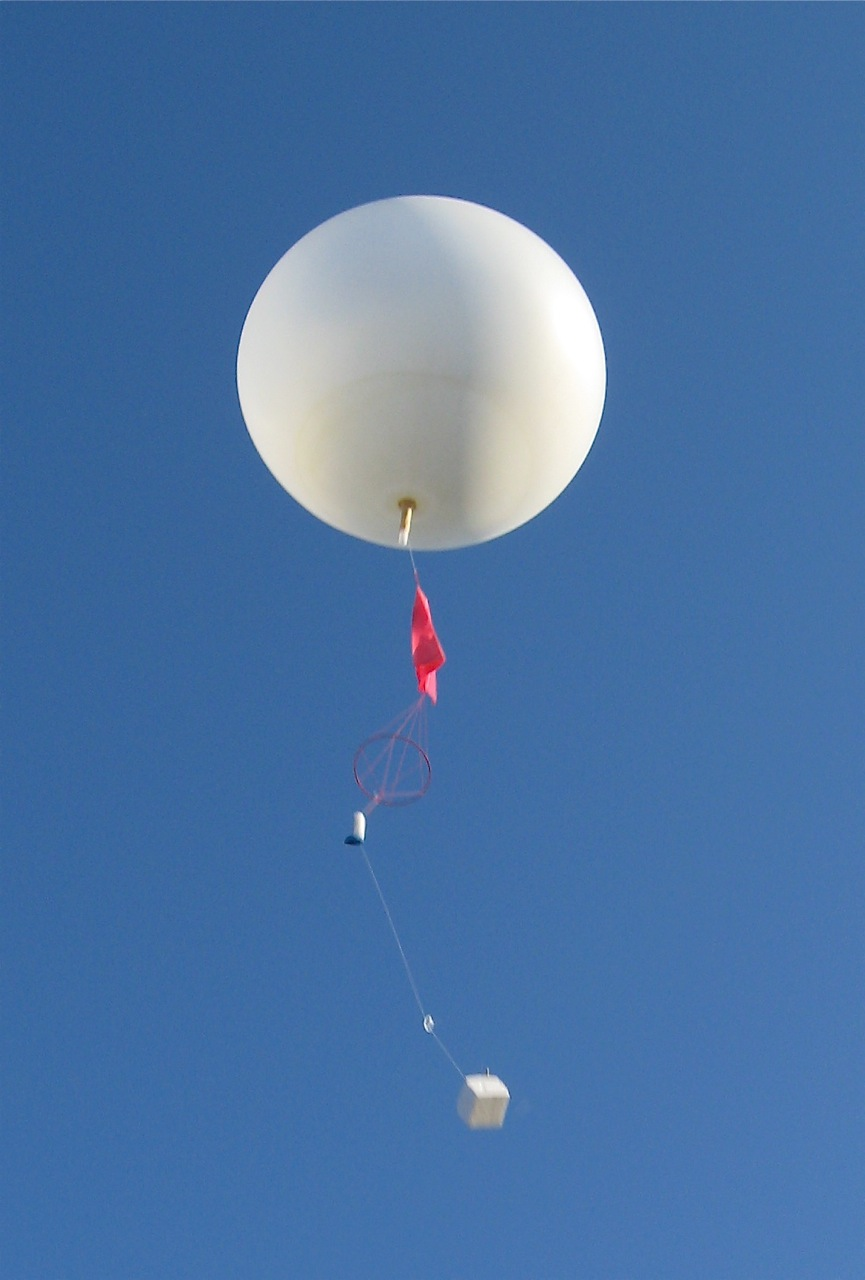
\includegraphics[width=0.6\linewidth]{Figures/Thermodynamics/Radiosonde 2.jpg}
    \caption{A Radiosonde! Also called a weather balloon/sounding balloon. It's released and floats upwards, continually measuring the pressure, temperature, and humidity of the air around it. Image from the Radiosonde Museum of North America \cite{Radiosonde}.}
    \end{subfigure}
    \hfill
    \begin{subfigure}{0.45\linewidth}
        \centering
        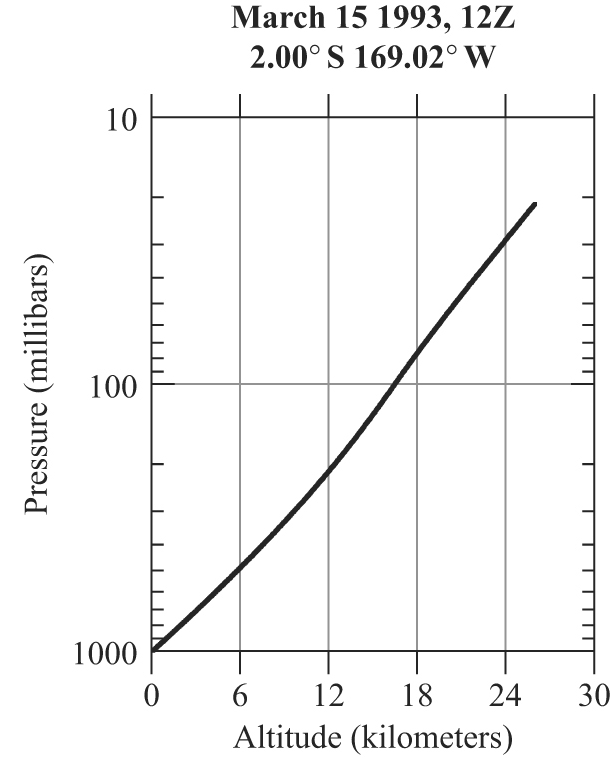
\includegraphics[width=0.8\linewidth]{Figures/Thermodynamics/Earth Radiosonde Pressure.png}
    \caption{Radiosonde measurement of the Earth. Note the log scale on the pressure axis, so if $p\sim e^{-z}$ we should expect a straight line, which we remarkably see. Notice how smooth the measurement is, despite the fact that it's a single radiosonde at a single  (horizontal) point in space. Figure from Ray's book \cite{Ray}.}
    \end{subfigure}
\end{figure}

\subsection{Example 3: Solid Rock Planet}

If we want to include curvature (since planets are more like spheres than infinite planes), we can derive an analogous \hyperref[Hydrostatic Balance]{Hydrostatic Relation} where:
\begin{align*}
    \frac{d p}{d r}&=-\rho g\\
    &=-\rho \frac{G M(r)}{r^{2}}
\end{align*}
We can couple this with a differential equation governing the mass below some radius $r$ called $M(r)$:
\begin{align*}
    \frac{d M}{d r} = 4\pi r^2\rho
\end{align*}

To solve these equations, as before, we need an expression for $\rho(r)$ and boundary conditions. $\rho(r)$ is typically given by the equation of state governing the material in question. For the Earth, for example, we might approximate $\rho\approx \text{const}$ below the ground ($r<R$) and $\rho$ as ideal as in \hyperref[Example 2: Ideal Gas]{Example 2} above the ground ($r>R$). For boundary conditions, we know that $M(r=0)=0$ and we can let $p(r=0)=p_0$ where $p_0$ is unknown. We can then integrate the equations, then solve for $p_0$ in terms of some other known reference pressure (e.g., if we know $p(r=r_s)=p_s$ we can write $p_0$ in terms of $p_s$).

\chapter{Dry Thermodynamics}\label{Dry Thermodynamics}

\section{The Vertical Structure of Atmospheres}\label{Vertical Structure}

We begin with some empirical observations of planetary atmospheres:

\begin{figure}[H]
    \begin{subfigure}[t]{0.24\linewidth}
        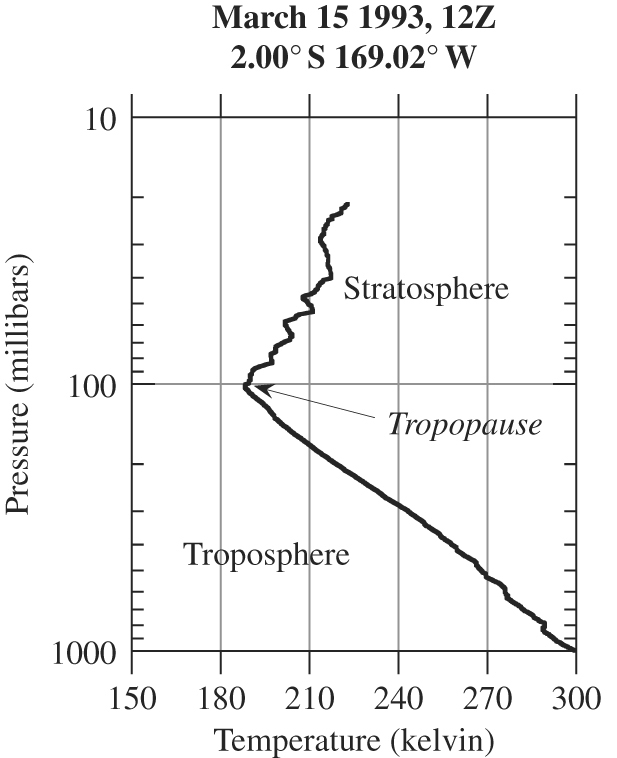
\includegraphics[width=\linewidth]{Figures/Thermodynamics/Earth Temperature Profile Radiosonde.png}
        \caption{Earth}
    \end{subfigure}
    \begin{subfigure}[t]{0.3\linewidth}
        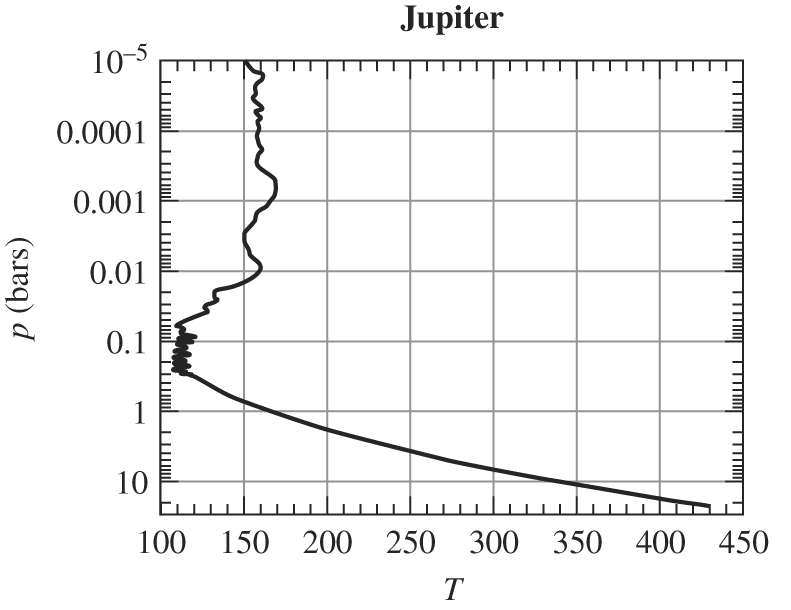
\includegraphics[width=\linewidth]{Figures/Thermodynamics/Jupiter Radiosonde.png}
    \end{subfigure}
    \begin{subfigure}[t]{0.3\linewidth}
        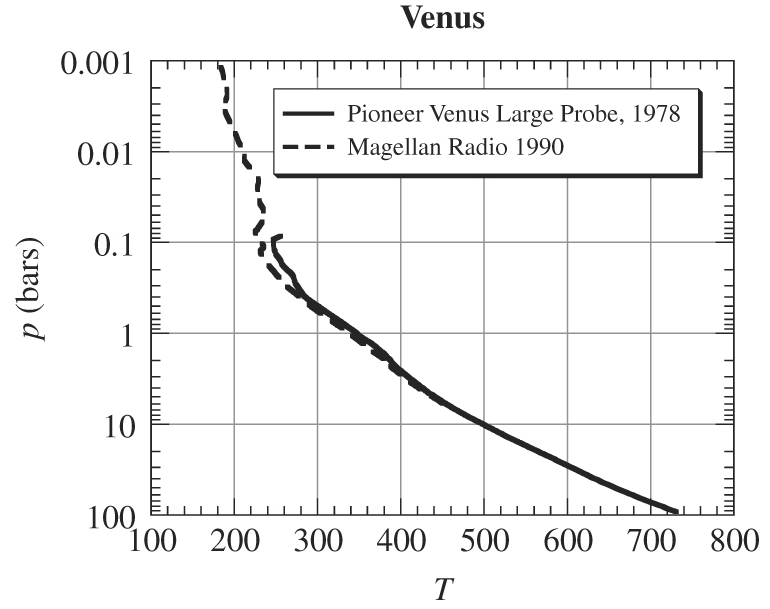
\includegraphics[width=\linewidth]{Figures/Thermodynamics/Venus Radiosonde.png}
    \end{subfigure}
    \centering
    \begin{subfigure}[b]{0.3\linewidth}
        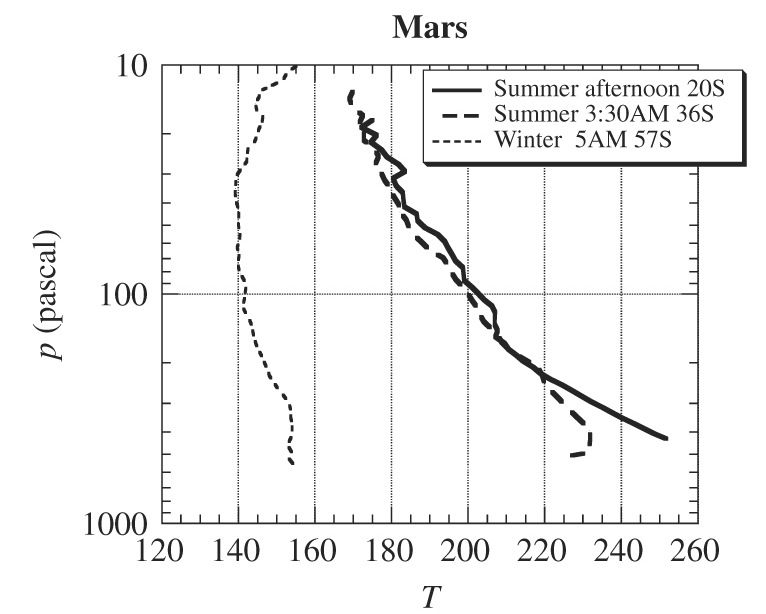
\includegraphics[width=\linewidth]{Figures/Thermodynamics/Mars Radiosonde.png}
    \end{subfigure}\quad
    \begin{subfigure}[b]{0.3\linewidth}
        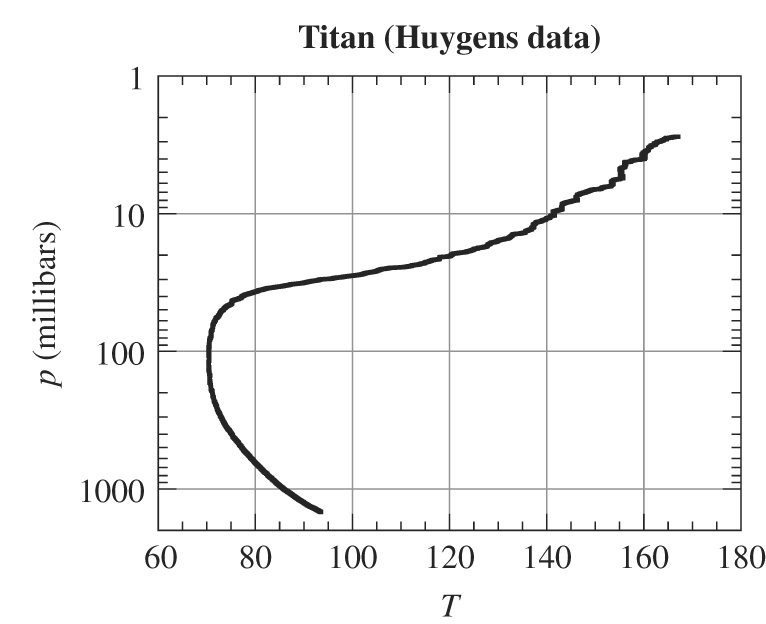
\includegraphics[width=\linewidth]{Figures/Thermodynamics/Titan Radiosonde.png}
    \end{subfigure}
    \caption{Vertical Temperature Profiles of Planets from Ray's book \cite{Ray}.}
\end{figure}

In all five plots, we see observe a sharp decrease of temperature with pressure in the lower portion of the atmosphere (which we call the \textbf{troposphere}), until a critical point (\textbf{tropoause}) in which the temperature decreases more slowly with height or even increases (\textbf{stratosphere})\footnote{
    I should note that I'm adhering to Ray's preferred terminology here. Ray uses \textbf{stratosphere} to refer to places in the atmosphere where radiative transfer is more dominant, which (we will see) causes a shallower decrease of temperature with height. This contrasts the more typical usage of the term \textbf{stratosphere}, which requires an increase of temperature with height. This only occurs if there is some heat source from above. In the case of the Earth, this heat source is due to the location of ozone, which is a very effective absorber of UV radiation. However, I prefer Ray's definition, due to reasons elaborated after I derive the \hyperref[Dry Adiabat Box]{Dry Adiabat} and the \hyperref[Dry Stability Box]{Dry Stability Criterion}. 
}.

In this chapter, we will attempt to explain this. We want to explain this because the vertical structure has profound consequences on many other phenomena of interest: the vertical structure affects, among other phenomena, where (or if) constituents condense (\hyperref[Moist Thermodynamics]{Moist Thermodynamics}), the outgoing radiation to space (\hyperref[Radiative Transfer]{Radiative Transfer}), and much of fluid dynamics (\hyperref[Geophysical Fluid Dynamics]{Geophysical Fluid Dynamics}). 

\noindent As a spoiler:
\begin{itemize}
    \item A temperature gradient is an indicator that there is an uneven heat source. The uneven heat source could be because:
    \begin{itemize}
        \item Radiation from the sun is absorbed unevenly. For example, on Earth, the ground absorbs much more visible light from the sun than the atmosphere, and ozone in the stratosphere absorbs much more UV light than the rest of the atmosphere.
        \item Energy is still leaking out from formation, as is the case with Jupiter.
    \end{itemize}
    \item The atmosphere redistributes heat away from the aforementioned uneven heat source. Heat is transferred \textit{down} the temperature gradient:
    \begin{itemize}
        \item If temperature decreases with height, the heat is coming from below.
        \item If temperature increases with height, the heat is coming from above.
    \end{itemize}
    \item There are two dominant heat transport mechanisms:
    \begin{itemize}
        \item Convection, which we will explain in this section. This is dominant in the \textbf{troposphere}.
        \item Radiation, which will explain in Part \ref{Radiative Transfer}. This is dominant in the \textbf{stratsophere}.
    \end{itemize}
\end{itemize}


\section{The Dry Adiabat: Rising and Falling Parcels of Air}

\subsection{Derivation}

To explain (some of) the aforementioned phenomenon, we start from the first law of thermodynamics governing a parcel of air:
\begin{align}
    \label{First Law}
    dU=-p\,dV+T\,dS+\mu\,dN
\end{align}
where $U=$ internal energy; $p=$ pressure; $V=$ volume; $T=$ temperature; $S=$ entropy; $\mu=$ chemical potential; and $N=$ number of molecules. Roughly, the $-p\,dV$ term corresponds to work done by the parcel (i.e., energy transferred by the parcel pushing or being pushed by its surroundings), $T\,dS$ corresponds to the heat transfer between the parcel and its surroundings, and $\mu\,dN$ corresponds to energy gained or lost by exchanging particles with its surroundings.

We assume that the system is closed ($dN=0$, so the parcel does not exchange air with its environment\footnote{This amounts to the assumption that entrainment does not occur. This is usually false, but it's not a bad assumption for what we aim to explain.}) and divide by the mass of the air parcel to find: 
\begin{align*}
    du=-p\,d\left(\frac{1}{\rho}\right)+T\,ds
\end{align*}
where $u$ and $s$ refer to the internal energy and entropy \textit{per unit mass} (remember, we want intensive variables only!). We now approximate the air parcel as an ideal gas. This means that:

\begin{enumerate}
    \item The gas obeys the Ideal Gas Law (\ref{Ideal Gas})
    \item The internal energy is a function of temperature only: $u=c_vT$, where $c_v=$ the specific heat capacity at constant volume.
    \item The specific heat capacities are related in the following way: $c_v+R=c_p$ (also per unit mass)
\end{enumerate}
\begin{align*}
    c_v\,dT&=-p\,d\left(\frac{1}{\rho}\right)+T\,ds
    &\text{; }&du=c_vdT \text{and assuming } \frac{\partial c_v}{\partial T}\approx0
    \\
    &=-p\,d\left(\frac{RT}{p}\right)+T\,ds
    &\text{; }&\text{Ideal gas using Eqn. \ref{Ideal Gas}}
    \\
    &=-pR\left(\frac{dT}{p}-\frac{T\,dp}{p^2}\right)+T\,ds
    &\text{; }&\text{Assume } \bar{M} \text{ is constant.}
    \\
    &=-R\,dT+\frac{RT\,dp}{p}+T\,ds
\end{align*}
Dividing by $T$ and rearranging, we find that:
\begin{align*}
    ds & = \frac{R_a+c_v}{T}\,dT+R\frac{dp}{p}
    \\
     & = c_p\,d\ln T-R\,d\ln p
     &\text{; }& d(\ln x)=\frac{dx}{x}\text{ and } R+c_v=c_p
     \\
     & = c_p\,d\left(\ln \left(T(p)^\frac{-R}{c_p}\right)\right)
     &\text{; }&\ln(x)-a\ln(y)=\ln\left(x(y)^{-a}\right)
\end{align*}
If we make the crucial assumption that the parcel exchanges a negligible amount of heat with its surroundings, then we can approximate $ds=0$\footnote{
    Why can we only approximate $ds=0$ and not set $ds=0$? It is because the relation $\dbar Q=T\,ds$ (where $\dbar Q$ is the heat transfer) holds only if the process is reversible, but we have made no such assumptions here. If the process is irreversible, as it probably is, then $\dbar Q\leq T\,ds$ and so it is possible for $\dbar Q=0$ and $ds\neq 0$.
}. In reality, there is some level of heat transfer ($ds\neq0)$, but these processes are typically much slower (timescale $\sim$ days/weeks) than the changes in pressure caused by upwards/downwards parcel motion (timescale $\sim$ hours). We can thus conclude that:
\begin{align*}
    0 & = c_p\,d\left(\ln \left(T(p)^\frac{-R}{c_p}\right)\right)\\
\end{align*}
and so we derive:
\begin{fact}{The Dry Adiabat}{Dry Adiabat Box}\label{Dry Adiabat Box}
The dry adiabat governs the temperature of an air parcel that is adiabatically lifted or dropped (due to, e.g., convection or dynamics). The temperature increases as pressure increases. This is because, as the parcel moves to a location where the ambient atmospheric pressure is higher, the atmosphere does work on the air parcel to compress it and increase its energy and therefore temperature.
    \begin{gather}
    \label{Dry Adiabat Slope}
    \BOX{
        \frac{d\ln T}{d\ln p}=\frac{R}{c_p}
    }\\
    \label{Dry Adiabat}
    \BOX{
        T(p)=T_0\left(\frac{p}{p_0}\right)^\frac{R}{c_p}
    }
    \end{gather}
If we crucially assume that \textbf{convection} is the \textbf{dominant vertical energy transport mechanism} in the atmosphere then the \textbf{atmosphere follows a dry adiabat}. This is somewhat accurate for Earth's troposphere.
\end{fact}
\subsection{Physical Interpretation}

Equation \ref{Dry Adiabat} is the \textbf{Dry Adiabat}. `\textbf{Dry}' because we have no condensation, and `\textbf{Adiabat}' because we assume $dS=0$ (and the word `adiabatic' refers to processes where $dS=0$). Constants $(p_0,T_0)$ refer to the initial temperature and pressure of the air parcel. 

Physically \ref{Dry Adiabat} corresponds to are parcel starting at some temperature and pressure ($T_0,p_0$) and being displaced upwards/downwards. When it is displaced upwards/downwards, it undergoes negligible diabatic heating and entrainment, so it's temperature does not change that way. However, when the ambient pressure changes, it expands/contracts, and the air parcel does positive/negative work on its surroundings. This \textit{decreases}/\textit{increases} the internal energy of the parcel, thus decreasing/increasing the temperature. That's why $T$ decreases as $p$ decreases in \ref{Dry Adiabat}. 

However, we should we wary of the limits of our conclusions here. Recall that we started this section considering an air parcel, not the entire atmosphere! We must make a final, crucial assumption that rising and falling air parcels (convection) is the dominant mechanism for heat transport within some domain in the atmosphere (e.g., from the ground to a certain height – for example the tropopause). \textit{This} implies that the temperature profile of the atmosphere within this domain follows the \textbf{Dry Adiabat}. If this domain extends to the ground, we may take the initial conditions initial conditions $(p_0,T_0)$ to be the temperature and pressure of the surface $(p_s,T_s)$.

However, not all planetary atmospheres and not even all of Earth's atmosphere obey this assumption. This assumption is not bad in the Earth's troposphere partly because here the atmosphere is heated from below: the atmosphere is transparent to the radiation from the sun, which penetrates through the atmosphere and heats the ground. The ground then heats the air above it, which becomes buoyant and convects. Similarly, Jupiter's internal energy leakage maintains a convective troposphere.

Finally, now, we can see now why many atmospheres have temperatures decreasing as pressure decreases or height increases. The first fact is readily noted from Eqn. \ref{Dry Adiabat}. We can show the second fact by combining the Dry Adiabat \ref{Dry Adiabat}, \hyperref[Hydrostatic Balance]{Hydrostatic Balance}, and \hyperref[Ideal Gas]{Ideal Gas} Ideal Gas to obtain an equation linking temperature with height:
\begin{align*}
    \frac{R}{c_p}&=\frac{d\ln T}{d\ln p}
    \\
    &=\frac{d T}{d z}\frac{p}{T}\frac{dz}{d p}
    &\text{; }& \text{chain rule}\\
    &=\frac{d T}{d z}\frac{p}{T}(-\rho g)^{-1} 
    &\text{; }& \text{\ref{Hydrostatic Balance}}
    \\
    &=\frac{d T}{d z}\frac{p}{T}\frac{RT}{p}(- g)^{-1}
    &\text{; }& \text{\ref{Ideal Gas}}
    \\
    &\therefore\,
    \boxed{\frac{dT}{dz}=-\frac{g}{c_p} = -\Gamma_d} &\text{; }& \Gamma_d=\text{ Dry Adiabatic Lapse Rate}\approx\text{\qty{10}{\kelvin\per\kilo\metre}}
\end{align*}

\begin{figure}[H]
    \centering
    \begin{subfigure}{0.6\linewidth}
        \centering
        \begin{tikzpicture}
            \draw[thick,->] (0,0) -- (4.5,0) node[anchor=north west] {$\ln T$};
            \draw[thick,->] (0,0) -- (0,4.5) node[anchor=south east] {$-\ln p$};
            \draw[ultra thick] (3,0) node[anchor=north] {$(\ln T_s,\ln p_s)$} -- (0,4);
            \node[circle,draw,fill=black,inner sep=0pt,minimum size =0.1cm] at (3,0){};
            \draw (1,1) node[anchor=north west] {$R$} -- (2.25,1);
            \draw (1,1) node[anchor=south east] {$c_p$} -- (1,2.67);
        \end{tikzpicture}
    \caption{The Dry Adiabat, as predicted by Equation \ref{Dry Adiabat}.}
    \end{subfigure}
    \begin{subfigure}{0.35\linewidth}
        \centering
        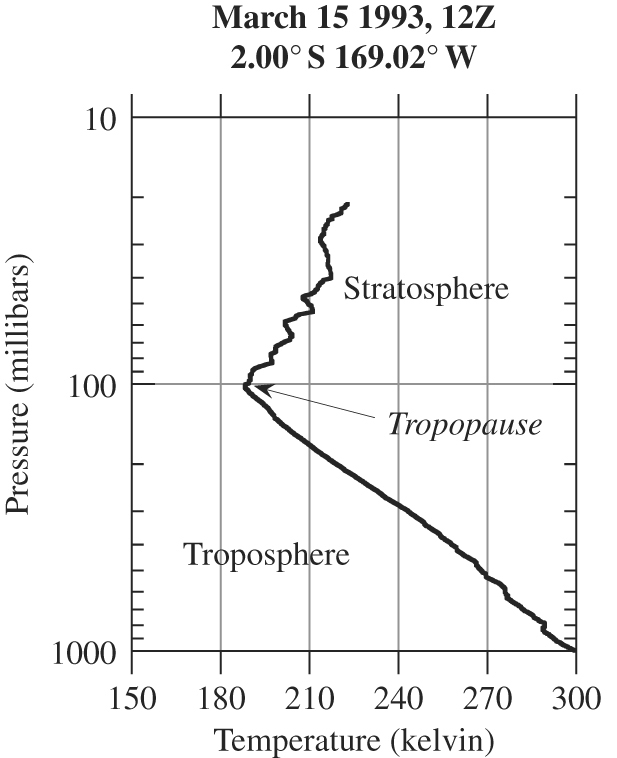
\includegraphics[width=0.8\linewidth]{Figures/Thermodynamics/Earth Temperature Profile Radiosonde.png}
    \caption{Radiosonde measurement of Earth's Temperature Profile.}
    \label{Earth T Observation}
    \end{subfigure}
    \caption{The Dry Adiabat: Theory v. Observation}
\end{figure}

Note that $R$ and $c_p$ have the same units/dimensions, so $\frac{R}{c_p}$ is dimensionless. We can use the \hyperref[Equipartition]{Equipartition Theorem} to estimate how quickly $T$ falls off with decreasing $p$. We know that $c_v\approx \frac{f}{2}R\approx\frac{5}{2}R$ for the Earth, and we know that $c_p\approx c_v+R$ for an ideal gas. Therefore, $c_p\approx \frac{7}{2}R$, so for the Earth:
\begin{align*}
    \frac{R}{c_p}\approx\frac{R}{\frac{7}{2}R}=\frac{2}{7}\approx\frac{d \ln T}{d \ln p}
\end{align*}

Of course, the atmosphere does not actually follow a \textbf{Dry Adiabat}, as clearly shown by Figure \ref{Earth T Observation}. It is somewhat accurate in the troposphere, but not so much elsewhere. That is because some of our assumptions were not as accurate as we would like. In reality, $dN\neq0$, and entrainment occurs, and $dS\neq0$, and diabatic heating occurs. Some of this diabatic heating is due to condensation, which we will learn how to deal with in the next chapter on \hyperref[Moist Thermodynamics]{Moist Thermodynamics}. Some of this is radiative heating, which we will discuss in the next part on \hyperref[Radiative Transfer]{Radiative Transfer}.

However, convection as a mechanism always perturbs an existing atmospheric profile to an \textbf{Adiabat}, and it is other processes (radiation, fluid dynamics) that pull the atmosphere away from an adiabat. In some cases, like in the \textbf{stratosphere}, radiation pulls the atmospheric profile to be super-stable, in which case convection is prohibited due to the stability of the atmosphere. In other cases, these other processes pull the atmospheric profile to be unstable, in which case convection takes over to push the atmosphere back to the \textbf{Adiabat}. What we have just touched upon is \hyperref[Radiative-Convective Equilibrium]{Radiative-Convective Equilibrium}, which we will discuss more in Part \ref{Clouds}.

\section{Potential Temperature}

In basic thermodynamics, we often introduce the concept of temperature operationally in the following way: suppose we have two objects $A$ and $B$, with temperatures $T_A$ and $T_B$, respectively, and we place them in contact with each other. Temperature encodes whether heat will flow, and in which way. If $T_A=T_B$, no heat will flow. If $T_B>T_A$, heat will flow from $B$ to $A$, and vice versa.

However, this will not work in atmospheric thermodynamics. Suppose we have two parcels of air called $A$ and $B$ at pressures $p_A$ and $p_B$\footnote{We are getting used to using pressure as a coordinate rather than height, remember!} with temperatures $T_A$ and $T_B$, respectively. Suppose we displace parcel $A$ in order to place it in contact with parcel $B$ (with no entrainment ($dN=0$) or diabatic heating ($dS=0$)).\newline

Which way will heat flow?\newline

We cannot naively use temperature as we did before, because parcel $A$'s temperature will change following the \hyperref[Dry Adiabat]{Dry Adiabat} as we move it to a different pressure. In other words, temperature is not a variable which is \hyperref[Material Conservation]{Materially Conserved} in Atmospheric/Oceanic Thermodynamics. A variable is \hyperref[Material Conservation]{Materially Conserved} if and only if it remains constant following a air/water parcel. This is a concept which will become very important in Part \ref{Geophysical Fluid Dynamics}.

We now want to define a quantity which serves the same role as temperature did before (i.e., a variable which encodes which way heat will flow) but which is \textit{also}, unlike temperature, \hyperref[Material Conservation]{materially conserved}. Let us consider a more general scenario, and move each parcel to some third pressure $p_{ref}$\footnote{Set $p_{ref}=p_B$ to recover our first example.}. 

We define the \textbf{Potential Temperature} $\theta$ as the temperature a parcel \textit{would} have if it were perfectly adiabatically moved to some reference pressure level $p_{ref}$:
\begin{align}\label{Potential Temperature}
    \BOX{\theta(T,p)=T\left(\frac{p}{p_{ref}}\right)^{-\frac{R}{c_p}}}
\end{align}
Recall that a few pages ago in our derivation of the \hyperref[Dry Adiabat]{Dry Adiabat} we found that:
\begin{align}
    ds=c_p\,d\left(\ln \left(T(p)^\frac{-R}{c_p}\right)\right)
\end{align}

Since the $\ln T(p)^\frac{-R}{c_p}$ term is within the differential, we can freely add and subtract constants within the differential, which corresponds to multiplying within the logarithm. We get then that:
\begin{align}
    ds&=c_p\,d\ln T\left(\frac{p}{p_{ref}}\right)^\frac{-R}{c_p}
    \\
    &=c_p\,d\ln\theta
\end{align}

As you can see, if $ds=0$, as we assumed during convection, then $d\theta=0$. Therefore, as we lift or drop a parcel, $\theta$ is \hyperref[Material Conservation]{materially conserved}.\footnote{In the Ocean, even without radiative heating processes, $\theta$ is not conserved. This is because there is a third thermodynamic state variable, salinity, which will change the temperature of sea water without adding any heat. Oceanographers have come up with another kind of materially conserved temperature in the ocean: \textit{Conservative Temperature}.}

Recalling that $TdS=dQ=$ heat, we find that the potential temperature is a measure of the extent to which diabatic/heat transfer processes have heated or cooled our parcel of air. It's essentially a measure of how wrong we were to assume that $dS=0$ in our derivation of \hyperref[Dry Adiabat]{Dry Adiabat}.

\section{Convection}\label{Convection}

\subsection{Buoyancy}

The atmosphere (and ocean) is a fluid, so even in the absence of most forces like friction, gravity is not the only force acting on a fluid parcel. There are also pressure gradient forces, which act to push fluid parcels away from areas of high pressure to areas of low pressure.

We already accounted for the effects of pressure in deriving \hyperref[Hydrostatic Balance]{Hydrostatic Balance} and the \hyperref[Dry Adiabat]{Dry Adiabat}. In the former case, the pressure gradient force acts to push fluid parcels upwards away from lower altitude regions of high pressure to higher altitude regions of low pressure in order to counteract the force of gravity on the ambient air. In the latter case, we only consider large-scale pressure gradients in the ambient atmosphere and we ignored pressure gradients across a fluid parcel.

Now we wish to take into account pressure gradients across a fluid parcel, and consider a fluid parcel which does \textit{not} have the same density as the air around it. Suppose we have a fluid parcel of density $m$ occupying some volume $V$. For simplicity assume the fluid parcel is rectangular, with a horizontal area of $A$ and a height of $h$ such that $V=Ah$.

Let us consider the forces per unit mass on the fluid parcel in the vertical direction. There are three forces of interest: the gravitational force $F_g=-g$, the pressure force on the \textit{bottom} pushing the parcel \textit{upwards} $F_{bot}=p(z)A/m$, and the pressure force on the \textit{top} pushing the parcel \textit{downards} $F_{top}=p(z+h)A/m$. $p(z)$ is the pressure at height $z$. The net force is then:
\begin{align*}
    F_z=-g-\frac{A}{m}(p(z+h)-p(z))
\end{align*}

We now make two assumptions. First, we assume that $h$ is small, therefore, $p(z+h)-p(z)\approx \frac{dp}{dz} h$. Second, we assume that the pressure in the fluid is set by \hyperref[Hydrostatic Balance]{Hydrostatic Balance}, therefore $p(z+h)-p(z)\approx \frac{dp}{dz} h=-\rho_a g h$, where $\rho_a$ is the density of the ambient air. We define $\rho_p=m/V$ as the density of the fluid parcel, and find that the total force on fluid parcel  is:
\begin{align}
    F_b&=-g+\frac{Ah}{m}\rho_a g\nonumber\\
    &=g\left( -1+ \frac{\rho_a}{\rho_p}\right)\nonumber\\
    \label{Buoyancy Force}
    \therefore \,\,& \BOX{F_b=g\left( \frac{\rho_a-\rho_p}{\rho_p} \right)}
\end{align}
where $F_b=$ the buoyancy force. Physically, the buoyant force is intuitive: if the air parcel is lighter than the ambient air ($\rho_p<\rho_a$) it will convect and rise, and vice versa. Furthermore, we can write $F_b$ in terms of the temperature $T$ (using \ref{Ideal Gas}) or potential temperature $\theta$ (using \ref{Potential Temperature}) in very neat forms, since many terms cancel top and bottom:
\begin{align}
    F_b=g\left( \frac{\rho_a-\rho_p}{\rho_p} \right)\nonumber\\
    \label{Buoyancy Force Temp}
    \boxed{F_b=g\left( \frac{T_p-T_a}{T_a} \right)}\\
    \boxed{F_b=g\left( \frac{\theta_p-\theta_a}{\theta_a} \right)}
\end{align}
So a parcel will convect if it is warmer or has a higher potential temperature than its ambient surroundings.

Finally, another way of thinking of the buoyant force is as a kind of `\textit{reduced gravity}'. The fluid acts like its on a planet of gravitational acceleration $g'=g\left( \frac{\rho_a-\rho_p}{\rho_p} \right)$ not $g$, and $g'<g$ always since $\rho_a>0$. This will be how we think of things in Chapter \ref{Shallow Water System}. 

\subsection{Convective Instability Criterion}

Now suppose we wish to find whether our atmosphere is convectively stable, i.e., whether the atmosphere will spontaneously undergo convection. If pressure and density did not appreciably change by height, then this would be easy: if $T(z)>T(z+c)$ where $c>0$ (and assuming that $\frac{\partial \rho}{\partial T}<0$), then we will have denser air overlying lighter air, and the parcels will convect.\footnote{
    This is the case if we're considering two layers of different temperature and composition that are in contact. This is because, at the point of contact, pressure changes only infinitessimaly, so the \hyperref[Dry Adiabat]{Dry Adiabat} is inapplicable (since $dp\approx0$). To determine whether these two layers are convectively stable, you must compare the densities directly, which depend on both the temperature of each layer and the molecular composition.
}

As before, the situation is a bit more complicated in an atmosphere when density and pressure vary significantly with height. Suppose again that we have an atmospheric temperature profile $T=T(p)$ (not necessarily following the dry adiabat). Suppose we lift a parcel at some pressure $p$ to some (smaller) pressure $p-\delta p$.

That parcel will be convectively unstable and continue rising if it is lighter (and therefore hotter) than the ambient surrounding air. We assume that the parcel is initially in equilibrium with its surroundings ($T_{parcel}(p)=T_{ambient}(p)$). We then Taylor Expand:
\begin{align*}
    T_{parcel}(p-\delta p)&>T_{ambient}(p-\delta p)\\
    {T_{parcel}(p)}-\frac{d T_{parcel}}{d p}\delta p & >T_{ambient}(p)-\frac{d T_{ambient}}{d p}\delta p\\
    \frac{d \ln T_{parcel}}{d \ln p} & <\frac{d \ln T_{ambient}}{d \ln p}
\end{align*}
Substituting in the \hyperref[Dry Adiabat]{Dry Adiabat} for $\frac{d \ln T_{parcel}}{d \ln p}$ we find the dry stability criterion:
\begin{fact}{The Dry Stability Criterion}{Dry Stability Box}\label{Dry Stability Box}
Suppose a dry atmosphere has a temperature profile $T(p)$. It will be:
\begin{multicols}{3}
    \centering
    Unstable to convection if:\newline
    \begin{align}\label{Dry Stability}
        \BOX{\frac{d\ln T}{d\ln p}>\frac{R}{c_p}}
    \end{align}
    Neutrally stable to convection if:
    \begin{align}
        \BOX{\frac{d\ln T}{d\ln p}=\frac{R}{c_p}}
    \end{align}
    and Stable to convection if:
    \begin{align}\label{Dry Stability Stable}
        \BOX{\frac{d\ln T}{d\ln p}<\frac{R}{c_p}}
    \end{align}
\end{multicols}
\end{fact}
Note that \ref{Dry Stability} and \ref{Dry Stability Stable} are not automatically ruled out due to \ref{Dry Adiabat}. That is because \ref{Dry Adiabat} governs a perfectly adiabatic rising/falling parcel of air. While this is the dominant contribution to the atmospheric temperature profile in the troposphere,  it is not the only one (even within the troposphere). Other processes (water vapour, radiation, dynamics) can push the atmospheric temperature profile away from the dry adiabat and make it stable or unstable. However, typically, unstable atmospheres are removed very quickly through spontaneous convection.

Physically, the idea is as follows: an atmosphere is stable if the temperature decreases slow enough with height (\ref{Dry Stability Stable}). If it decreases too quickly (\ref{Dry Stability}), a lifted parcel of air will have cooled \textit{less} than its surroundings, and thus be warmer and lighter than its surroundings, and continue to rise due to buoyancy (\ref{Buoyancy Force Temp}).

If \ref{Dry Stability Stable} obtains then an atmosphere will be \textit{super-stable} and will inhibit convection. A quick sanity check to remember which way the inequality is in \ref{Dry Stability} is the following: an isothermal\footnote{
    `Iso' meaning same and `thermal' meaning temperature, so `Isothermal' means constant temperature.
} atmosphere is always super-stable. An isothermal atmosphere will have $\frac{d \ln T}{d \ln p} = 0$, so $\left( \frac{d \ln T}{d \ln p} < \frac{R}{c_p} \right)$ corresponds to instability. If one has a \textit{super-stable} atmosphere then that indicates that there has been some other dominant energy transport mechanism that has kept the atmosphere in this state. This is characteristic of a \textbf{stratosphere}.\footnote{
    Recall the footnote on \hyperref[Vertical Structure]{this} page. This is why Ray prefers that definition of \textbf{stratosphere}: a stratsophere should be characterised by what energy transport mechanism is dominant, not whether it happens to have shortwave absorbers.
} 

\begin{figure}[H]
    \centering
    \begin{tikzpicture}
        \begin{scope}
            \draw[thick,->] (0,0) -- (4,0) node[anchor=south] {$\ln T$};
            \draw[thick,->] (0,0) -- (0,4) node[anchor=south east] {$-\ln p$};
            \draw[ultra thick] (3,0) node[anchor=north] {$(\ln T_s,\ln p_s)$} -- (0,3);
            %\draw[ultra thick] (3,0) node[anchor=north] {$(\ln T_s,\ln p_s)$} -- (0,4);
            \node[circle,draw,fill=black,inner sep=0pt,minimum size =0.1cm] at (3,0){};
            \node[circle,draw,fill=red,inner sep=0pt,minimum size =0.2cm] (A) at (1.5,1.5){};
            \node at (2.5,2.5){Unstable};
            \node[] (B) at (2.4,0.3){};
            \node[] (C) at (0.6,2.7){};
            \draw[thick,red] (B) -- (C);
        \end{scope}
        \begin{scope}[xshift=5.5cm]
            \draw[thick,->] (0,0) -- (4,0) node[anchor=south] {$\ln T$};
            \draw[thick,->] (0,0) -- (0,4) node[anchor=south east] {$-\ln p$};
            \draw[ultra thick] (2.625,0) node[anchor=north] {$(\ln T_s,\ln p_s)$} -- (0,3.5);
            %\draw[ultra thick] (3,0) node[anchor=north] {$(\ln T_s,\ln p_s)$} -- (0,4);
            \node[circle,draw,fill=black,inner sep=0pt,minimum size =0.1cm] at (2.625,0){};
            \node[circle,draw,fill=red,inner sep=0pt,minimum size =0.2cm] (A) at (1.5,1.5){};
            \node at (2.5,2.5){Neutrally Stable};
            \node[] (B) at (2.4,0.3){};
            \node[] (C) at (0.6,2.7){};
            \draw[thick,red] (B) -- (C);
        \end{scope}
        \begin{scope}[xshift=11cm]
            \draw[thick,->] (0,0) -- (4,0) node[anchor=south] {$\ln T$};
            \draw[thick,->] (0,0) -- (0,4) node[anchor=south east] {$-\ln p$};
            \draw[ultra thick] (1.5,0) node[anchor=north] {$(\ln T_s,\ln p_s)$} -- (1.5,3);
            %\draw[ultra thick] (3,0) node[anchor=north] {$(\ln T_s,\ln p_s)$} -- (0,4);
            \node[circle,draw,fill=black,inner sep=0pt,minimum size =0.1cm] at (1.5,0){};
            \node[circle,draw,fill=red,inner sep=0pt,minimum size =0.2cm] (A) at (1.5,1.5){};
            \node at (2.5,2.5){Stable};
            \node[] (B) at (2.4,0.3){};
            \node[] (C) at (0.6,2.7){};
            \draw[thick,red] (B) -- (C);
        \end{scope}
    \end{tikzpicture}
    \caption{Dry Stability: From left to right: unstable, neutrally stable, and super stable atmospheric temperature profiles. Thick black is the atmospheric profile, thin red is the dry adiabatic slope.}
\end{figure}


\begin{comment}
    \subsection{Enthalpy and Conservation of Enthalpy}
    
    Consider a box of air that undergoes convection. The total energy $U$ contained within that box of air which is the sum of the kinetic energy ($\frac{1}{2}v^2$), the internal energy ($c_v T$), and potential energy ($gz$):
    
    \begin{align*}
        U = \int\int\int \left(\frac{1}{2}v^2+c_v T+gz\right)\rho\,dz\,dx\,dy
    \end{align*}
    
    Let us assume that that system is closed: there is no (net) radiative heating and cooling and no flow in and out of that box. This is good assumption, given how fast convection is. We further assume that there kinetic energy is negligible both before and after convection occurs. Therefore, $U$ is conserved over the entire box, and $\Delta U=0$. We finally assume that the initial and final states are hydrostatic. Therefore:
    
    \begin{align*}
        \int\int\int gz \rho\,dz\,dx\,dy
    \end{align*}
    
    \begin{align*}
        U &= \int\int\int \left(c_v T+gz\right)\rho\,dz\,dx\,dy\\
        &=\int\int\int \left(c_v T+gz\right)\rho\,dz\,dx\,dy
    \end{align*}
    
    We define (specific) enthalpy as follows:
    
    \begin{align}
        h=u+p\left( \frac{1}{\rho} \right)
    \end{align}
    
    \noindent Taking the differential of enthalpy, then applying the hydrostatic relation:
    
    \begin{align*}
        dh & = du + dp \left( \frac{1}{\rho} \right) - p\, d \left( \frac{1}{\rho} \right)\\
        & = T\,ds + p\, d \left( \frac{1}{\rho} \right) + dp \left( \frac{1}{\rho} \right) - p\, d \left( \frac{1}{\rho} \right)\\
        & = T\,ds + dp \frac{1}{\rho}\\
        & = T\,ds - g \, dz
    \end{align*}
\end{comment}

\subsection{Convective Stability Criterion with Potential Temperature}

We can formulate an equivalent criterion for potential temperature. Recall that if two parcels of air have potential temperatures $\theta_A$ and $\theta_B$ such that $\theta_A>\theta_B$, then parcel $A$ will have a higher temperature than parcel $B$ if they're at the same pressure.

We can very straightforwardly derive an equivalent criterion for convective instability, this time in terms of potential tempreature $\theta$, by rearranging \ref{Potential Temperature} for $T(\theta)$ and substituting that into \ref{Dry Stability}.
\begin{comment}
    We can therefore naturally extend the derivation for \ref{Dry Stability}, using instead properties of potential temperature, noting that $T_{parcel}=T(\theta_{parcel}(p),p)$ and $T_{ambient}=T(\theta_{ambient}(p))$.
    
    \begin{align*}
        T_{parcel}(p-\delta p)&>T_{ambient}(p-\delta p)\\
        {T_{parcel}(p)}-\frac{\partial T_{parcel}}{\partial p}\delta p - \frac{d T_{parcel}}{d \theta_{parcel}}\frac{d\theta_{parcel}}{dp}\delta p
        & >T_{ambient}(p)-\frac{d T_{ambient}}{d \theta_{ambient}}\frac{d\theta_{ambient}}{dp}\delta p\\
        -\frac{d T_{parcel}}{d p}\delta p
        & >-\frac{d T_{ambient}}{d \theta_{ambient}}\frac{d\theta_{ambient}}{dp}\delta p\\
        \frac{d \ln T_{parcel}}{d \ln p} & <\frac{d \ln T_{ambient}}{d \ln p}
    \end{align*}
    
    A slightly more straightforward but maybe less physically intuitive derivation starts directly by rearranging \ref{Potential Temperature} for $T(\theta)$ and substituting that into \ref{Dry Stability}.
\end{comment}
\begin{align*}
    1&<\frac{c_p}{R}\frac{d\ln T(\theta)}{d\ln p}
    &\text{ ; }&\text{\ref{Dry Stability}}
    \\
    &=\frac{c_p}{R}\frac{d\ln \left( \theta\left( \frac{p}{p_{ref}} \right)^{\frac{R}{c_p}} \right)}{d\ln p}
    &\text{ ; }&\text{substitute \ref{Potential Temperature}}
    \\
    &=\frac{c_p}{R} \left( 
        \frac{d \ln \theta}{d \ln p}+
        \frac{d \ln \left(p^{\frac{R}{c_p}} \right)}{d \ln p}+
        \frac{d \ln \left(p_{ref}^{\frac{-R}{c_p}} \right)}{d \ln p}
     \right)
    &\text{ ; }&\text{split logarithm}
    \\
    &=\frac{c_p}{R}\frac{p}{\theta}\frac{d\theta}{dp}+\frac{c_p}{R}\frac{R}{c_p}
    &\text{ ; }
    &\ln p^{R/c_p}=R/c_p\ln p
\end{align*}
Therefore, since $\theta>0$ and $p>0$ always, we get that our atmosphere is unstable if and only if:
\begin{align}\label{Dry Stability Potential Temperature}
    \boxed{\frac{d\theta}{dp}>0}
\end{align}
Using the hydrostatic relation and the fact that $g>0,\rho>0$, we get our criterion for instability in height coordinates:
\begin{align}
    \BOX{\frac{d\theta}{dz}<0}
\end{align}

Therefore, if potential temperature decreases with height, then our atmosphere is unstable. This makes physical sense. Recall that potential temperature takes the place of temperature in atmospheric thermodynamics, in the sense that it is potential temperature that stays the same when you lift/drop and air parcel. If you lift an air parcel, its potential temperature stays the same. However, if the ambient potential temperature decreases with height, then it will be colder than the air parcel, and the air parcel will keep rising. 

\begin{figure}[H]
    \centering
    \begin{tikzpicture}
        \begin{scope}
            \draw[thick,->] (0,0) -- (4,0) node[anchor=south] {$\theta$};
            \draw[thick,->] (0,0) -- (0,4) node[anchor=south east] {$z$};
            \draw[ultra thick] (3,0) node[anchor=north] {$(\theta_s,0)$} -- (0,3);
            %\draw[ultra thick] (3,0) node[anchor=north] {$(\ln T_s,\ln p_s)$} -- (0,4);
            \node[circle,draw,fill=black,inner sep=0pt,minimum size =0.1cm] at (3,0){};
            \node[circle,draw,fill=red,inner sep=0pt,minimum size =0.2cm] (A) at (1.5,1.5){};
            \node at (2.5,3.5){Unstable};
            \node[] (B) at (1.5,0.3){};
            \node[] (C) at (1.5,2.7){};
            \draw[thick,red] (B) -- (C);
        \end{scope}
        \begin{scope}[xshift=5.5cm]
            \draw[thick,->] (0,0) -- (4,0) node[anchor=south] {$\theta$};
            \draw[thick,->] (0,0) -- (0,4) node[anchor=south east] {$z$};
            \draw[ultra thick] (1.5,0) node[anchor=north] {$(\theta_s,0)$} -- (1.5,3);
            %\draw[ultra thick] (3,0) node[anchor=north] {$(\ln T_s,\ln p_s)$} -- (0,4);
            \node[circle,draw,fill=black,inner sep=0pt,minimum size =0.1cm] at (1.5,0){};
            \node[circle,draw,fill=red,inner sep=0pt,minimum size =0.2cm] (A) at (1.5,1.5){};
            \node at (2.5,3.5){Neutrally Stable};
            \node[] (B) at (1.5,0.3){};
            \node[] (C) at (1.5,2.7){};
            \draw[thick,red] (B) -- (C);
        \end{scope}
        \begin{scope}[xshift=11cm]
            \draw[thick,->] (0,0) -- (4,0) node[anchor=south] {$\theta$};
            \draw[thick,->] (0,0) -- (0,4) node[anchor=south east] {$z$};
            \draw[ultra thick] (0,0) node[anchor=north west] {$(\theta_s,0)$} -- (3,3);
            %\draw[ultra thick] (3,0) node[anchor=north] {$(\ln T_s,\ln p_s)$} -- (0,4);
            \node[circle,draw,fill=black,inner sep=0pt,minimum size =0.1cm] at (0,0){};
            \node[circle,draw,fill=red,inner sep=0pt,minimum size =0.2cm] (A) at (1.5,1.5){};
            \node at (2.5,3.5){Stable};
            \node[] (B) at (1.5,0.3){};
            \node[] (C) at (1.5,2.7){};
            \draw[thick,red] (B) -- (C);
        \end{scope}
    \end{tikzpicture}
    \caption{Dry Stability: From left to right: unstable, neutrally stable, and super stable atmospheric temperature profiles. Thick black is the atmospheric profile, thin red is the dry adiabatic slope.}
\end{figure}

\subsection{CAPE, LFC, LNB}

We have so far characterised \textit{whether} convection will occur in our dry atmosphere, but now we wish to know what will happen \textit{during} convection. We start again by considering a parcel of air at an initial pressure $p_0$ with a temperature of $T_p(p_0)$. Let $T_a(p)$ be the temperature profile of the ambient atmosphere, and assume that initially the parcel is in equilibrium with its surroundings (i.e., assume $T_p(p_0)=T_a(p_0)$).

We define the \textbf{L}evel of \textbf{F}ree \textbf{C}onvection (\textbf{LFC}) $p_{LFC}$ as the \textit{first} location where $T_p(p)=T_a(p)$. We define the \textbf{L}evel of \textbf{N}eutral \textbf{B}uoyancy (\textbf{LNB}) as the \textit{second} location where $T_p(p)=T_a(p)$.

We define the \textbf{C}onvective \textbf{A}vailable \textbf{P}otential \textbf{E}nergy (\textbf{CAPE}) as the total available potential energy (per unit mass) for a parcel of air from the Level of Free Convection to the Level of Neutral Buoyancy. In other words, $CAPE$ is equal to the total kinetic energy per unit mass a parcel would gain if it was allowed to convect from the Level of Free Convection to the Level of Neutral Buoyancy:
\begin{align}
    CAPE=\int_{z_{LFC}}^{z_{LNB}}F_b\,dz
\end{align}
We can substitute for $F_b$ using \ref{Buoyancy Force Temp} and convert to pressure coordinates using \ref{Hydrostatic Balance Ideal} to find that:
\begin{gather*}
    CAPE=\int_{z_{LFC}}^{z_{LNB}}\frac{T_p-T_a}{T_a}g\,dz\\
    =\int_{p_{LFC}}^{p_{LNB}}\frac{T_p-T_a}{\bcancel{T_a}}(-R\bcancel{T_a}\,d\ln p)\\
    \therefore \boxed{CAPE=R\int_{p_{LNB}}^{p_{LFC}}\left( T_p-T_a \right)\,d\ln p}
\end{gather*}
We know $T_p(p)$, since $T_p(p)$ follows the \hyperref[Dry Adiabat]{Dry Adiabat} with $(p_0,T_0)=(p_{LFC},T_{LFC})$, so we can straightfowardly calculate $CAPE$ if we are given the atmospheric temperature profile $T_a(p)$.

We further define \textbf{C}onvective \textbf{IN}hibition (\textbf{CIN}) as the energy a fluid parcel would need to overcome to reach the \textbf{LFC}:
\begin{align*}
    \boxed{CIN = R\int_{p_{LFC}}^{p_{0}}\left( T_p-T_a \right)\,d\ln p}
\end{align*}
We expect $CIN<0$ and $CAPE>0$. Above \textbf{LNB}, we expect there to be more `$CIN$', which will prevent the parcel from rising further. However, at this point, the parcel will have already gained kinetic energy from $CAPE$. We call where the parcel `stops' the \textbf{L}evel of \textbf{M}aximum \textbf{A}scent (\textbf{LMA}), which occurs at $p_{LMA}$ where the `$CIN$' above \textbf{LNB} equals the $CAPE$:
\begin{align*}
    \boxed{
        R\int_{p_{LMA}}^{p_{LNB}}\left( T_p-T_a \right)\,d\ln p = 
        R\int_{p_{LNB}}^{p_{LFC}}\left( T_p-T_a \right)\,d\ln p
    }
\end{align*}

\begin{fact}{Convection Definitions}{Convection Box}\label{Convection Box}
    Let the ambient air temperature be $T_a(p)$ (black line \textcolor{black}{\rule{0.25cm}{0.25cm}}). Consider an air parcel at an initial pressure $p_0$ with a temperature of $T_p(p_0)=T_a(p_0)$ that is then lifted. Upon lifting, the parcel's temperature $T_p(p)$ follows the \hyperref[Dry Adiabat]{Dry Adiabat} (\textcolor{mymagenta}{dashed magenta line \rule{0.25cm}{0.25cm}}). Then:
    \begin{quote}
        \textbf{Level of Free Convection} (\textbf{LFC}): $p=p_{LFC}$ if $T_p(p)=T_a(p)$, $dT_p/dp<dT_a/dp$, and this is the first pressure $p<p_0$ where this occurs.

        \textbf{Level of Neutral Buoyancy} (\textbf{LNB}): $p=p_{LNB}$ if $T_p(p)=T_a(p)$, $dT_p/dp>dT_a/dp$, and this is the first pressure $p<p_0$ where this occurs.

        \textbf{Level of Maximum Ascent} (\textbf{LMA}): $p=p_{LMA}$ where $p_{LMA}$ is determined by Equation \ref{LMA} (I.e., where the blue area \textcolor{mydarkblue}{\rule{0.25cm}{0.25cm}} equals the orange area \textcolor{myorange}{\rule{0.25cm}{0.25cm}}).
    \end{quote}

    \noindent\begin{minipage}{.48\linewidth}
        \begin{align}
        \label{CAPE}
        \BOX{CAPE=R\int_{p_{LNB}}^{p_{LFC}}\left( T_p-T_a \right)\,d\ln p}\\
        \label{CIN}
        \BOX{CIN=R\int_{p_{LFC}}^{p_{0}}\left( T_p-T_a \right)\,d\ln p}\\
        \label{LMA}
        \BOX{R\int_{p_{LMA}}^{p_{LNB}}\left( T_p-T_a \right)\,d\ln p = CAPE}
    \end{align}
    \end{minipage}
    \hspace{5mm}
    \begin{minipage}{.48\linewidth}
    \begin{figure}[H]
        \centering
        \begin{tikzpicture}
            \draw[->] (0,0) -- (4.5,0) node[anchor=west]{$T$};
            \draw[->] (0,0) -- (0,4.5) node[anchor=south]{$-\ln p$};
            \coordinate (ps) at (4.2,0);
            \node[] at (4.2,-0.4) {$p_s$};
            \coordinate (p0) at (4,0.5);
            \node[] at (4.35,0.5) {$p_0$};
            \coordinate (end) at (0,4.5);
            \coordinate (LFC) at (2.7,1.8);
            \node[] at (3.1,2.1) {\textbf{LFC}};
            \node[] at (2.7,1) {$CIN$ \textcolor{myyellow}{\rule{0.25cm}{0.25cm}}};
            \coordinate (LNB) at (1.3,3.2);
            \node[] at (0.8,3) {\textbf{LNB}};
            \coordinate (LMA) at (0.8,4.5);
            \node[] at (1.6,4.5) {\textbf{LMA}};
            \node[] at (2.7,2.8) {$CAPE$ \textcolor{mydarkblue}{\rule{0.25cm}{0.25cm}}};
            %\filldraw[fill=green!50] (p0) .. controls +(0,1) and +(1,0) .. (LFC);
            \filldraw[thick,fill=myyellow] (p0) .. controls +(0,1) and +(1,0) .. (LFC);
            \filldraw[thick,fill=mydarkblue] (LFC) .. controls +(-1,0) and +(0,-1) .. (LNB);
            \path[fill=myorange] (LNB) .. controls +(0,0.5) and +(0.5,-0.5) .. (LMA) -- (end);
            %\filldraw[fill=myorange] 
            \draw[dashed,mymagenta,thick] (p0) -- (end);
            \node[circle,draw,fill=black,inner sep=0pt,minimum size =0.15cm] at (ps){};
            \node[circle,draw,fill=black,inner sep=0pt,minimum size =0.15cm] at (p0){};
            \node[circle,draw,fill=black,inner sep=0pt,minimum size =0.15cm] at (LFC){};
            \node[circle,draw,fill=black,inner sep=0pt,minimum size =0.15cm] at (LNB){};
            \node[circle,draw,fill=black,inner sep=0pt,minimum size =0.15cm] at (LMA){};
            \draw[thick] (ps) .. controls +(0,0.1) and +(0,-0.5) .. (p0);
            \draw[thick] (LNB) .. controls +(0,0.5) and +(0.5,-0.5) .. (LMA);
        \end{tikzpicture}
        \caption{Atmospheric Profile. The parcel is lifted from $p_0$. $CIN$ is proportional to the area shaded in \textbf{\textcolor{myyellow}{Yellow \rule{0.25cm}{0.25cm}}} and $CAPE$ is proportional to the area shaded in \textcolor{mydarkblue}{\textbf{Blue} \rule{0.25cm}{0.25cm}}.}
    \end{figure}
    \end{minipage}
\end{fact}

\subsection{Conservation of Enthalpy during Convection}

We define the (specific) \textbf{Enthalpy} $h$ as follows:
\begin{align}
    h=u+p\frac{1}{\rho}
\end{align}
For an ideal gas, we can substitute for $p$ using \ref{Ideal Gas} and $u=c_vT$ to write $h$ in terms of $T$ only:
\begin{align*}
    h&=\underbrace{c_vT}_{u}+\underbrace{\rho R T}_{p}\frac{1}{\rho}\\
    &=\underbrace{(c_v+R)}_{c_p}T\\
    &=c_pT
\end{align*}
Therefore we can interpret the enthalpy $h$ as an expression of the heat content of a system at constant pressure, like for example in the atmosphere.

We introduce the enthalpy because we can show that, under suitable assumptions, the total enthalpy $H$ of an atmospheric column is conserved during convection:
\begin{align*}
    H=\iiint \rho h\,dV=const
\end{align*}
We make three assumptions:
\begin{enumerate}
    \item The initial and final states are both in Hydrostatic Balance \ref{Hydrostatic Balance}
    \item The kinetic energy of the initial and final state is negligible compared to the potential and internal energy.
    \item No mass or heat leaves domain.
\end{enumerate}
The last assumption requires some elaboration. First, we \textit{don't} assume that no energy leaves the domain: we allow the column to do work on the air above or below itself as it expands/contracts. Second, we \textit{don't} assume that there is no heating within the column. In fact, we expect there to be some heating within the column in general: If a column is convectively unstable, then there will be \textbf{CAPE}, and we expect this to be converted into an appreciable amount of kinetic energy as the air parcels within the column convect. Once convection acts to remove the \textbf{CAPE}, we expect friction to slow the parcels down and convert the kinetic energy into heat. 

We first consider the total energy in an atmospheric column per horizontal area between altitudes $z_0$ and $z_1$, which is the sum of the internal energy $u$ and the potential energy $gz$ (and we have assumed kinetic energy $\frac{1}{2}v^2$ is negligible):
\begin{align*}
    E &= \int_{z_0}^{z_1} \rho \left( u + gz \right)dz\\
    &=\frac{1}{g}\int_{p_1}^{p_0} \left( u+gz \right)dp
\end{align*}
We then integrate the potential energy term $gz$ by parts:
\begin{align*}
    g\int_{p_1}^{p_0} z\,dp &= g\left[ zp \right]_{p_0}^{p_1}-g\int_{z_1}^{z_0}p\,dz\\
    &=g(z_0p_0-z_1p_1)+\int_{p_1}^{p_0}\frac{p}{\rho}dp
\end{align*}
Therefore the total energy per unit area is:
\begin{align*}
    E=\frac{1}{g}\int_{p_1}^{p_0}\left(u+\frac{p}{\rho} \right)\,dp+(z_0p_0-z_1p_1)
\end{align*}
We make a final, fourth assumption here that the pressure at the bottom $p_0$ and top $p_1$ of the column is unchanged between the final and initial states. This is ensured if we assume the entire column (inside and outside the column under consideration) is in hydrostatic balance and the mass of the air above, within, and below the column under consideration is unchanged (recall \ref{Hydrostatic Differential}). The change in energy $\Delta E$ between the final and initial states is then:
\begin{align}
    \label{Delta E 1}
    \Delta E = \frac{1}{g}\Delta \int_{p_1}^{p_0}h\,dp + p_0 \Delta z_0 - p_1 \Delta z_1
\end{align}
We now wish to equate this with the change in energy of the atmospheric column governed by \ref{First Law}. Since we have assumed that there is no heat or mass transfer to or from the system, we can set $dN=0$ and approximate $dS=0$. Therefore, the change in energy (per unit area), to a good approximation, is set by:
\begin{align}
    dE &= -p\,dV/A\nonumber\\
    &=p_0 d z_0-p_1 d z_1\nonumber\\
    \label{Delta E 2}
    \therefore \Delta E & = p_0 \Delta z_0 - p_1 \Delta z_1 
\end{align}
Therefore, setting \ref{Delta E 1} equal to \ref{Delta E 2} we can cancel the $p\Delta z$ to find that:
\begin{align}
    \BOX{\Delta H = \Delta \iiint \rho h \,dz\,dx\,dy=0}
\end{align}
The enthalpy of a column is conserved under convection. If we assume that the atmosphere is an ideal gas (so that $h=c_pT$) and that $c_p$ is approximately independent of temperature (so that we can pull $c_p$ out of the integral), then we can convert to pressure coordinates to find that:
\begin{align*}
    H =  \int \int \frac{c_p}{g} \int  T \,dp\,dx\,dy
\end{align*}
Therefore we find that the enthalpy is proportional to $\int T\,dp$, and so:
\begin{align}
    \boxed{
        \Delta \int T dp = 0
    }
\end{align}
during convection.

\begin{comment}
    We can take the differential of this to find the following relation:
    \begin{align*}
        dh&=du+dp\frac{1}{\rho}+p\,d\left( \frac{1}{\rho} \right)\\
        &=\underbrace{Tds-\bcancel{p\,d\left( \frac{1}{\rho} \right)}}_{du}+dp\frac{1}{\rho}+\bcancel{p\,d\left( \frac{1}{\rho} \right)}\\
        &=Tds+\frac{1}{\rho}dp
    \end{align*}
\end{comment}

\chapter{Moist Thermodynamics}\label{Moist Thermodynamics}

\section{Phase Transitions}

In the previous chapter, we considered only atmospheres made up completely of constituents that do not undergo any phase transitions. However, Earth's atmosphere (and many others) clearly do not obey this assumption. Earth's atmosphere has a non-negligible amount of condensible substances: water vapour (look outside and you might see a cloud!), which clearly condense, evaporate, and freeze in Earth-like conditions.

So what is a phase transition? We will only be dealing with so-called \textbf{First-Order Phase Transitions}, which occur when there is a \textit{discontinuity} in a thermodynamic state variable and an absorption or release of a large amount of energy, called \textbf{latent heat}. Phase transitions occur at certain temperatures and pressures\footnote{Whether a phase transition will occur might also depend on other thermodynamic state variables. For example, salinity is a thermodynamic variable which affects when sea water evaporates.}. We can represent this with a \textbf{Phase Diagramme}, as shown below:

\begin{figure}[H]
    \centering
    \begin{subfigure}{0.45\linewidth}
        \centering
        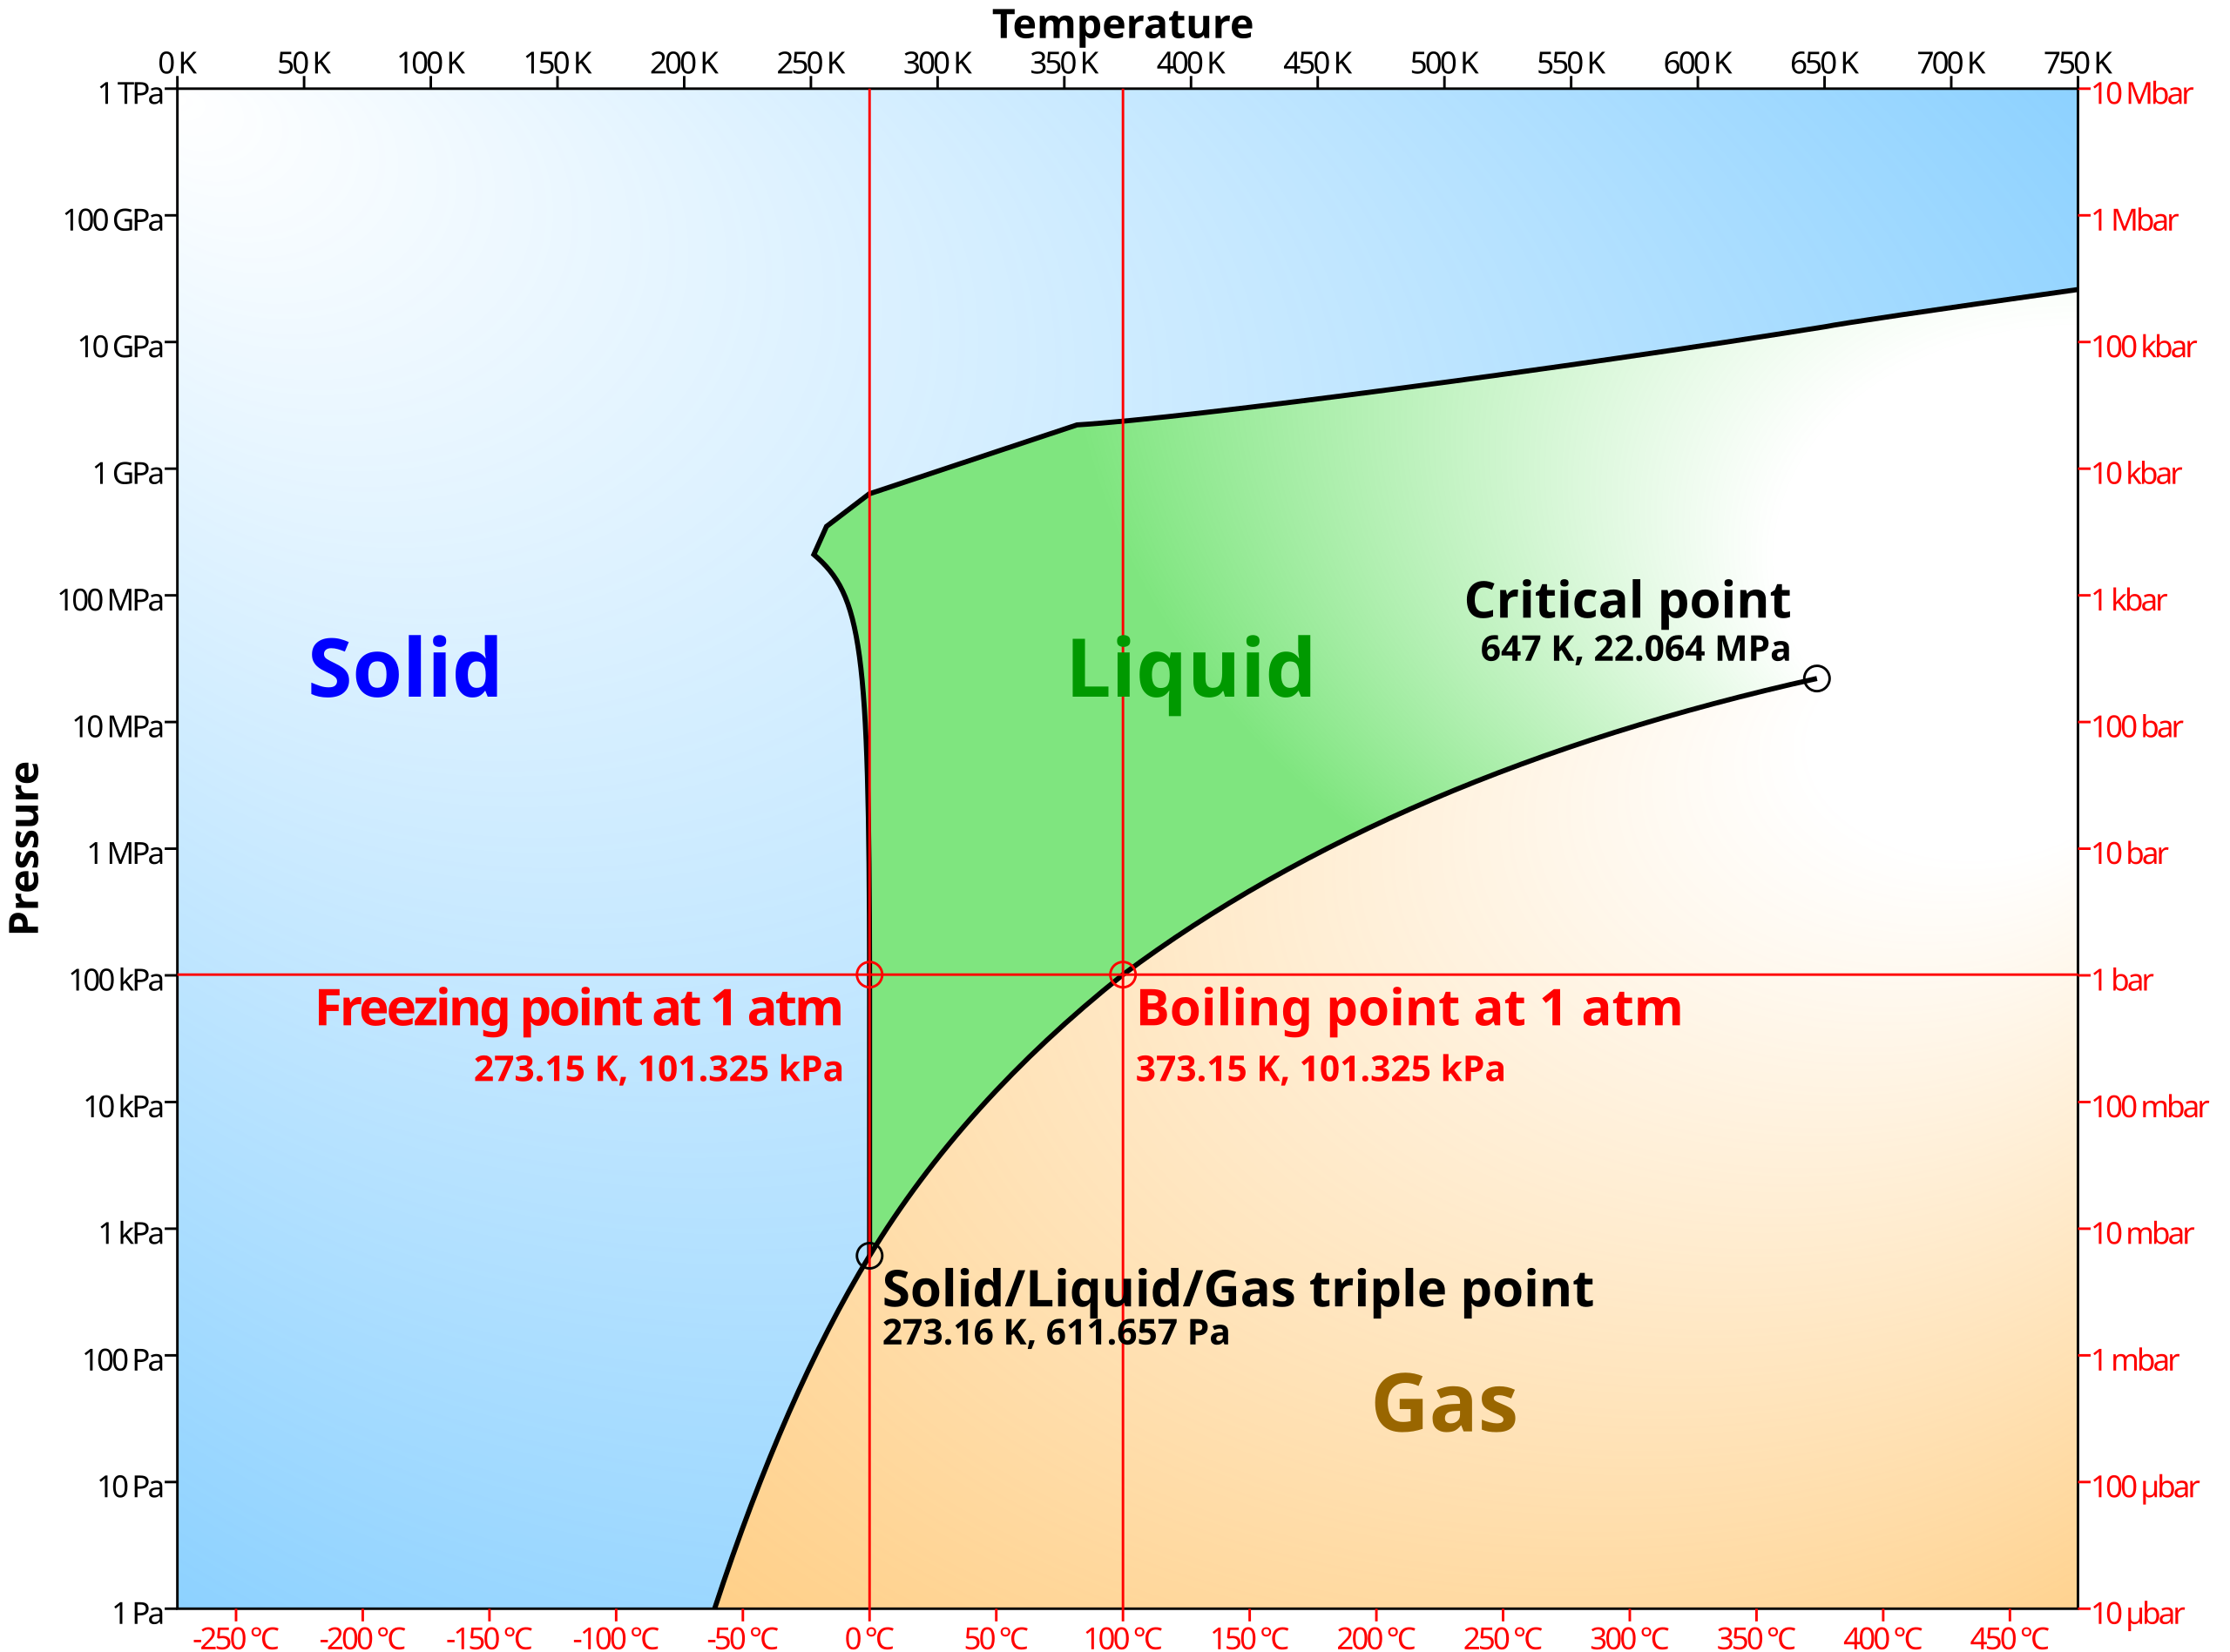
\includegraphics[width=\linewidth]{Figures/Thermodynamics/Phase_diagram_of_water_simplified.svg.png}
    \end{subfigure}
    \begin{subfigure}{0.45\linewidth}
        \centering
        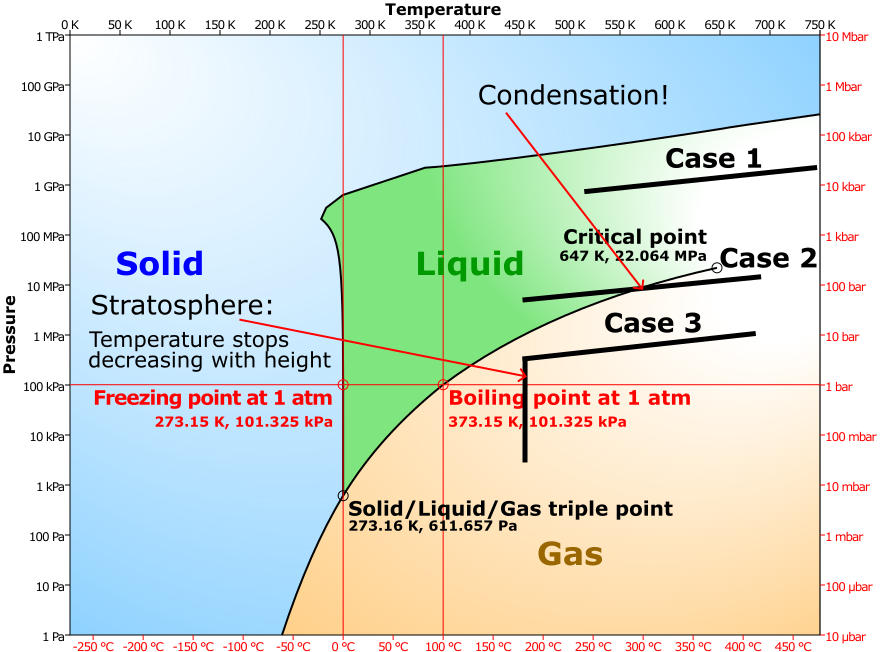
\includegraphics[width=\linewidth]{Figures/Thermodynamics/Phase_diagram_of_water_simplified.png}
    \end{subfigure}
    %\includesvg{Figures/Thermodynamics/Phase_diagram_of_water_simplified}
    \caption{Phase Diagramme for Water from Wikipedia \cite{PhaseDiagramme}.}
    \label{Phase Diagramme}
\end{figure}

Focus on the left-hand plot for now. The coloured regions indicate what phase water will be in at a certain the partial pressure (of the water) and temperature: gas (vapour), liquid (steam), and solid (ice). Crucially, this does not depend on the total pressure of the atmosphere or surrounding gases, but only the partial pressure of the condensible substance (in this case, the partial pressure of water). The solid black lines indicate \textbf{Phase Boundaries}. The \textbf{Triple Point} is a point where all three states can coexist. The \textbf{Critical Point} is the point past which there is no phase transition between gas and liquid.

The pressure at the \textbf{Phase Boundaries} is the \textbf{Saturation Vapour Pressure} $p_{sat}(T)$. If the partial pressure $p<p_{sat}$, then more vapour (gas form) can be added without condensing. If the $p\geq p_{sat}$, then the gas will condense until the partial pressure reaches the saturation vapour pressure. However, it's important to remember that condensation is not instantaneous, which is partly why we can have atmospheric conditions where $p>p_{sat}$. This will be important when we consider \hyperref[Clouds]{Clouds}.

In fact all gases can condense if the temperature is low enough/partial pressure is high enough. CO$_2$ can condenses on Mars, and N$_2$ condenses on Neptune. Why doesn't CO$_2$ and N$_2$ condense here on Earth? It all depends on the vertical structure of the atmosphere: the precise profile of $T=T(p)$. Recall that, as $p$ decreases, so too does $T$ (if our atmosphere follows the \hyperref[Dry Adiabat]{Dry Adiabat}). There are three cases, all labeled in the right-hand plot of Figure \ref{Phase Diagramme}.

\begin{enumerate}
    \item Case 1: The atmosphere has such a high pressure/temperature that it avoids a phase transition altogether by meandering around the critical point.
    \item Case 2: The atmospheric profile cuts right through a phase boundary, and the condensible condenses (clouds form!).
    \item Case 3: The stratosphere starts before the atmosphere hits the phase boundary, in which case temperature no longer decreases with height, so it never crosses the phase boundary.
\end{enumerate}

For O$_2$ and N$_2$ in Earth like conditions, we are in case 3: it never gets cold enough for O$_2$ and N$_2$ to condense, which is why we have no O$_2$ and N$_2$ clouds. However, we are in Case 2 with water (H$_2$O), and so we do get water clouds!

When a gase condenses from phase $A$ to phase $B$, it typically releases a large amount of \textbf{Latent Heat}. Again, we would like to work in intensive variables, so we often work with the \textbf{Specific Latent Heat} $L_{A\to B}$ (units of \qty{}{\joule\per\kilogram}) which is the amount of energy released per kilogram of substance when underoing a phase transition from $A$ to $B$ ($L_{A\to B}>0$ if heat is released). Like heat capacity, this often has a temperature dependence, but we will in most cases treat this as constant.

\section{The Clausius-Clapeyron Relation}

We can derive the shape of the phase boundary with the \textbf{Clausius Clapeyron Relation}, which relates the saturation vapour pressure to the temperature using the latent heat and the densities. We will not derive it here, but it would be useful for you to memorise the following relation:
\begin{align}\label{Clausius Clapeyron}
    \BOX{
        \frac{dp_{sat}}{dT}=\frac{L_{A\to B}}{T\left(\frac{1}{\rho_A}-\frac{1}{\rho_B}\right)}
        }
\end{align}
If we assume that $\rho_g\ll\rho_l$ (i.e., the gaseous form is much less dense than the liquid form), and that the gas is ideal, we find that:
\begin{align}
    \frac{d p_{sat}}{dT}&\approx\frac{L_{g\to l}}{T \frac{1}{\rho_g}}\nonumber\\
    & = \frac{L_{g \to l} p}{R_cT^2}\nonumber\\
    \therefore \,\,\,& \boxed{\frac{d \ln p_{sat}}{d \left( \frac{1}{T} \right)} \approx -\frac{L_{g\to l}}{R_c}}\label{Clausius Clapeyron Simplified}
\end{align}

Note that I have written $R_c$ to make clear that $R_c$ is the specific gas constant for the condensible (e.g., water) \textit{not} for the atmosphere. We can now derive an analytic expression for the saturation vapour pressure if we further assume that the latent heat is constant. 
\begin{align}
    \boxed{
        p_{sat}\approx p_0 \,e^{\frac{L}{R_c}\left( \frac{1}{T_0}-\frac{1}{T} \right)}
    }
    \label{Sat Vap Pressure}
\end{align}
where I now just write $L$ for the latent heat of condensation and $(T_0,p_0)$ are any point on the saturation vapour pressure curve. This could be, for example, the \textbf{triple point} or the \textbf{critical point}.

As we can see then, the saturation vapour pressure depends approximately \textit{exponentially} on temperature, so saturation vapour pressure decreases exponentially as temperature decreases. Conversely, if saturation vapour pressure decreases, T changes only logarithmically (i.e., very slowly).

\section{The Moist Pseudo-Adiabat: Lifting Moist Parcels of Air}\label{Moist Pseudo Adiabat}

Our goal now is to derive an analogous \hyperref[Dry Adiabat]{Dry Adiabat} relation for moist atmospheres consisting of some condensible substance $c$. We call this the \textbf{Moist Pseudo-Adiabat}. We call this a `\textit{Pseudo}'-Adiabat because we assume, for mathematical convenience, that the condensible substance $c$ is instantaneously removed from the air parcel. This can occurs if, for example, $c$ instantaneously rains out (but rain is not the only way in which this may occur!). When the condensible is removed, this constitutes a diabatic process ($dN\neq 0$), so strictly speaking we will not derive an adiabat in this section.

In reality, rising moist air parcels that condense will not instantaneously eject its condensed $c$, and so will not follow the pseudo-adiabat. However, the pseudo-adiabat is a good approximation if the amount of condensate left in the air parcel is small, which is at least the case on Earth.

Recall that we are using the same logic as we did before in deriving the \hyperref[Dry Adiabat]{Dry Adiabat}. As such, we are still assuming that the dominant mechanism of heat transport within the atmosphere is vertical convection, only this time the air parcels convecting are moist (have condensible substances in them). 

We will now consider two limiting cases. In both cases, we make the crucial assumption that the air parcels remain saturated with the condensible. In other words, we assume that the partial pressure of the condensible is equal to the saturation vapour pressure $p_{sat}$.

\subsection{Limit I: Single Component Condensible Atmosphere} 

We consider the first limiting case, with an atmosphere made up wholly of one condensible substance $c$. Since there is only one constituent, the total pressure is equal to the partial pressure of the $c$. There are two possibilities now.

The first possibility obtains if the surface at the ground (and therefore partial pressure at the ground) is too high ($p_g>p_{sat}(T_g)$). Then there will be an ocean of $c$ at the surface. The pressure within the ocean will obey \hyperref[Hydrostatic Balance]{Hydrostatic Relation}, and the surface of the ocean is determined by where the pressure and temperature intersect the phase boundary ($p=p_s=p_{sat}(T_s)$).

The temperature above the surface of the ocean is set by convecting air parcels. These air parcels originate from the surface of the ocean, and are initially saturated. However, recall that we have assumed that the air parcel remains saturated.\footnote{
    I'm not sure how justified this assumption is. I plan to ask Ray about this at some point, but if this footnote is still here when you're reading it I have not (yet).
} As such, the atmospheric profile must lie on the phase boundary, so the temperature is fixed to the phase boundary and is as follows (found by rearranging \ref{Sat Vap Pressure} for $T$ in terms of $p_{sat}$):
\begin{align}
    \text{If } p_g>p_{sat(T_g)}\text{: }& T(p)=\frac{T_s}{1-\frac{RT_s}{L}\ln\frac{p}{p_{s}}} \label{1 component moist adiabat} \\
    &p_s = p_{sat}(T_s)
\end{align}

The surface pressure $p_s$, then, is set by the surface temperature $T_s$. Recalling Equation \ref{Total Mass Hydrostatic}, the mass of the atmosphere is set by how hot it is. Physically, this corresponds to how much of $C$ you can evaporate from the ocean!

Second, if the surface at the ground is too low ($p_g=p_s<p_{sat}(T_s)$), then there will be no surface $c$ ocean, and the  atmosphere will follow the \hyperref[Dry Adiabat]{Dry Adiabat} until it reaches the phase boundary at the \textbf{lifted condensation level}, after which it will follow Equation \ref{1 component moist adiabat}:
\begin{align}
    \text{If } p_s<p_{sat(T_s)}\text{: }
    &
    T(p)=
    \begin{cases}
        T_s\left(\frac{p}{p_s}\right)^\frac{R}{c_p} \text{ for }p<p_{LCL}\\
        \frac{T_s}{1-\frac{RT_s}{L}\ln\frac{p}{p_{LCL}}}, \text{ for }p>p_{LCL}
    \end{cases}\\
    \text{where }&p_{LCL}=p_{sat}\left( T_s\left(\frac{p_{LCL}}{p_s}\right)^\frac{R}{c_p} \right)
\end{align}

In other words, the temperature follows the Dry Adiabat until the \textbf{lifted condensation level}. We can solve for the pressure at the \textbf{lifted condensation level} by finding where the Dry Adiabat intersects the phase boundary (the latter of which is calculated using \hyperref[Clausius Clapeyron]{Clausius Clapeyron}).

\subsection{Limit II: Dilute Condensible}

\subsubsection{Derivation}

We now consider the second limiting case, where the atmosphere is mainly made up of a non-condensible substance $a$, and a dilute condensible substance $c$. We follow a similar derivaiton to the \hyperref[Dry Adiabat]{Dry Adiabat}, and start from the first law of thermodynamics, but this time include the extra latent heat term $-L\,dq$:
\begin{align}\label{1st law latent heat}
    du=-p\,d\left(\frac{1}{\rho}\right)+T\,ds-L\,dq
\end{align}

\noindent where $L=$ the latent heat of condensation and $q=\frac{\rho_c}{\rho_a}$ the mass mixing ratio of $c$ in its gaseous form (and \textit{not} the $c$ in its liquid form, which we assume (recall) are removed from the parcel of air). For water, $q=$ the mass mixing ratio of the water vapour and the dry air, \textit{not} the water droplets and the dry air. In the dilute limit, $q\ll 1$, and $q$ is equal to the mass fraction. 

Take care to note the assumptions we're making here, and what the letters we've written actually mean. $u$, $\rho$, $T$,  and $s$ refer to properties of $a$ in the parcel of air, while $p$ refers to the total pressure of both the $a$ and $c$. Here we are implicitly making three assumptions. First, we assume that we are in the dilute limit $q\ll 1$, therefore $\rho=\rho_a+\rho_c\approx\rho_a$. Second, we assume the heat capacities of $a$ and $c$ are of similar size, and that therefore the specific internal energy $u$ is primarily made up of the internal energy of $a$.

As a sanity check, let us consider the minus sign on the $L\,dq$ term. This makes physical sense: we expect the internal energy of the $a$ to \textit{increase} if condensation occurs, since latent heat is released when $c$ condenses, and heat is added to $a$ in the air parcel. If condensation occurs, then the mass of the liquid $c$ (e.g., water droplets) must increase, and therefore (by mass conservation) the mass of the gaseous $c$ (e.g., water vapour) must decrease. Therefore, the mass mixing ratio of $c$ must decrease, so $dq<0$, therefore $-L\,dq>0$, as expected.

Let us first consider the $L\,dq$ term:
\begin{align*}
    L\,dq&=L\, d \left( \frac{\rho_c}{\rho_a} \right)\\
        &=L\, d \left( \frac{M_c e}{M_a (p-e)} \right)\\
        &\approx L\, d \left( \frac{M_c}{M_a} \frac{e}{p} \right)\\
    L\,dq&\approx L \,\epsilon \,d \left( \frac{e}{p} \right)
\end{align*}

\noindent where $\rho_c=$ the density of the condensible $c$; $\rho_a=$ the density of the air $a$; $M_c=$ the molar mass of the condensible; $M_a=$ the molar mass of the air; $p=p_a+p_c=$ the total pressure; $e=p_c=$ the partial pressure of the condensible; $\epsilon=\frac{M_c}{M_a}= $ the ratio of molar masses $c$ and $a$.

\noindent We can now apply product rule and assume that the condensible is always saturated. This allows us to use the simplified version of Clausius Clapyeron (\ref{Clausius Clapeyron Simplified}) to simplify things.
\begin{align*}
    L\,dq &\approx L \,\epsilon \,d \left( \frac{e}{p} \right)\\
    &= L \, \epsilon \left( \frac{de}{p} - \frac{e}{p^2}dp \right)
    &\text{; }
    &\text{Chain Rule}
    \\
    &= L\,\epsilon\frac{e}{p}\left( \frac{de}{e} - \frac{dp}{p} \right)
    \\
    &=Lq\,d\ln p_{sat}-Lq\,d\ln p
    &\text{; }
    &q\approx L\,\epsilon \frac{e}{p} \text{ and assume } e\approx p_{sat}
    \\
    &=-q\frac{L^2}{R_c}\,d\left( \frac{1}{T} \right)-Lq\,d\ln p
    &\text{; }
    &\text{Clausius Clapeyron \ref{Clausius Clapeyron Simplified}}\\
    &=q\frac{L^2}{R_c T^2}\,dT-Lq\,d\ln p\\
    &=q\frac{L^2}{R_cT}\,d\ln T-Lq\,d\ln p
\end{align*}

\noindent We now subsitute this into \ref{1st law latent heat} and, for simplicity, let $ds=0$ from the outset.\footnote{We could allow $ds\neq 0$ and derive what's called an \textbf{Equivalent Moist Potential Temperature} $\theta_E$ (analogous to \hyperref[Potential Temperature]{Potential Temperature} $\theta$), which is similarly \hyperref[Material Conservation]{materially conserved} for moist saturated parcels of air. We don't for brevity, but if you wish to read up more on it, here is a resource: whoops I forgot to insert the link, please let me know if this is still here!} Following identical algebra in the derivation of the \hyperref[Dry Adiabat]{Dry Adiabat}, and carefully distinguishing between $R_a$ and $R_c$ (the specific gas constants of the non-condensible and dilute condensible), we find that:
\begin{align*}
    c_v\,dT & =-R_a\,dT+\frac{R_aT\,dp}{p}-L\,dq\\
    \therefore c_p\,dT &= \frac{R_a T\,dp}{p} - q\frac{L^2}{R_cT}\,d\ln T+Lq\,d\ln p\\
    \therefore c_p\,d\ln T - \frac{q L^2}{R_c T^2}d\ln T&=R_a\,d\ln p + \frac{Lq}{T}d\ln p
\end{align*}

\noindent Solving for $\frac{d\ln T}{d\ln p}$ and rearranging, we the \textbf{Moist Pseudo-Adiabat} in the dilute limit:
\begin{fact}{Dilute Moist Pseudo-Adiabat}{Moist PA Box}\label{Moist PA Box}
    The adiabat for an atmosphere consisting of a dilute condensible is as follows:
    \begin{align}\label{dilute moist adiabat}
        \BOX{\frac{d\ln T}{d\ln p}=\frac{R}{c_p^a}\frac{1+\frac{L\,q_{sat}}{R_aT}}{1+\frac{L\,q_{sat}}{c_p^aT}\frac{L}{R_cT}}}
    \end{align}
    This is in general a \textit{shallower} slope than the \hyperref[Dry Adiabat Box]{Dry Adiabat} due to the latent heat of condensation keeping the parcel warm.
\end{fact}

\noindent where I have written $q=q_{sat}$ and $c_p=c_p^a$ to remind us that, first, we have made the crucial assumption that the air parcel remains saturated, and second, that $c_p$ is the heat capacity of the non-condensible $a$.

\subsubsection{Physical Interpretation}

Equation \ref{dilute moist adiabat} is, in general, not analytically solvable. However, we have written it in the form that provides easy interpretation. The first term is the slope of the adiabat if there were no condensation (the \hyperref[Dry Adiabat]{Dry Adiabat}), while the second complicated looking fraction are the changes in the slope due to condensation. Setting $q=0$ recovers the Dry Adiabat.

Note that although we have made the dilute assumption that $q\ll 1$, the corrections on the right hand side are generally of order $1$. This is because the corrections go as $\frac{L q_{sat}}{R_a T}$ and $\frac{Lq_{sat}}{c_p T}\frac{L}{R_cT}$, and it is gernally the case that, for water vapour on Earth at least, $\frac{L}{R_a T}\gg 1$.

It is almost always the case (although I cannot show algebraically) that the moist adiabat is shallower than the dry adiabat, i.e., that temperature decreases less with a decrease in pressure (and increase in height): 

\begin{align*}
    \frac{d\ln T_{moist}}{d\ln p} < \frac{d\ln T_{dry}}{dp}
\end{align*}

Physicsally, this corresponds to to the effect of the condensible. As a parcel rises, the pressure decreases, so it expands and cools (following the dry adiabat). However, since the temperature decreases, so too does the saturation vapour pressure (\ref{Clausius Clapeyron}). So if the parcel is saturated, as we have assumed, $c$ must condense and release latent heat into the surrounding air parcel, warming it a bit and offsetting the cooling from expansion.

Finally, we must note that we have made the assumption that the parcel remains saturated. In general, this will be the case for rising saturated parcels of air, which will only condense so much as to remain approximatly saturated. However, if a parcel is \textit{sinking}, then clearly it is not always realistic to assume that it will automatically acquire some more water vapour to remain saturated. As such, if a parcel of air is sinking, it will most likely follow the \hyperref[Dry Adiabat Box]{Dry Adiabat}. 

\subsubsection{What Happens if $q<q_{sat}$?}

Suppose we start an air parcel off sub-saturated (i.e., $q<q_{sat}$, initially). What temperature profile will it follow as it is lifted? 

Initially, as it is lifted, its mass mixing ratio $q$ will remain constant, and its temperature will decrease following the \hyperref[Dry Adiabat]{Dry Adiabat}. This will continue until the temperature has cooled so much (following the Dry Adiabat) causing the saturation vapour pressure to decrease sufficiently such that $q=q_{sat}$. After this point, it will follow the \hyperref[dilute moist adiabat]{Dilute Moist Pseudo-Adiabat}.

\subsection{Moist Convection}

Ideas from Section \ref{Convection} carry over to here, but are changed subtly. However, to avoid repetition, please refer to Chapter \ref{Convection Clouds}.

\part{Radiative Transfer}\label{Radiative Transfer}

\section*{Introduction}

This section of the course was lectured by \href{https://users.physics.ox.ac.uk/~pierrehumbert/}{Raymond T. Pierrehumbert} covering basic atmospheric Radiative Transfer. In the academic year 2024-2025, Ray did not cover scattering, so I will not cover scattering in these notes.\vspace{5 mm}

\noindent This section consists of four chapters:\vspace{5 mm}

\begin{enumerate}
    \item \hyperref[Basic Thermodynamics]{Basic Radiation Concepts}: 
        
        \begin{quote}
            We introduce the basic vocabulary needed to describe radiative transfer. We first characterise the radiation field, including how to encode the \hyperref[Solid Angle Box]{direction} and \hyperref[Radiance Box]{magnitude} of radiation. Next, we describe how objects emit and absorb radiation.
        \end{quote}

    \item Molecular Spectroscopy: 
    
        \begin{quote}
            We detail how we characterise \hyperref[Line Box]{spectral lines} in terms of certain parameters. We then discuss how those parameters are determined physically, and introduce some explicit functional forms such as the \hyperref[Lorentz Box]{Lorentz Line Shape}.
        \end{quote}
    
    \item Schwarzschild Equation:
        
        \begin{quote}
            We formulate an equation for radiative transfer throughout the atmosphere and solve it. We  
        \end{quote}
    \item Radiative Equilibrium:
        
        \begin{quote}
            We make the grey gas approximation in order to analyse how an atmosphere would behave in pure radiative equilibrium: i.e., if radiation were the dominant energy transport mechanism.
        \end{quote}
\end{enumerate}

\chapter{Basic Radiation Concepts}

\section{Direction of Radiation: Rays and Solid Angle}

In general, radiation will not only be a function of position $\vec{r}$ but will also be a function of direction\footnote{This is why your eyes will hurt if you look directly at the sun but they won't if you look at these lecture notes.}. We can encode the direction in which radiation is propagating with a \textbf{ray}, a vector $\vec{\omega}$ of (dimensionless) length $1$ on a unit sphere. $\vec{\omega}$ encodes information regarding the direction of propagation, but not regarding the magnitude (e.g., energy) of the radiation. In Cartesian coordinates, this is:
\begin{align}
    \vec{\omega}=\left(\begin{array}{ccc}
         \sin(\theta)\cos(\phi)\\
         \sin(\theta)\sin(\phi)\\
         \cos(\theta)
    \end{array}\right)
\end{align}

We also define the \textbf{Solid Angle}, which is a measure of a set of rays, with units of \textbf{Steradians} (\qty{}{\steradian}). In other words, \textbf{solid angle} encodes from \textit{how many} directions some radiation is coming from. For example, if radiation is propagating towards you from every direction, the \textbf{solid angle} of that will be larger than if radiation were only propagating towards you from a single direction.

We can make this more intuitive by drawing an analogy between the solid angle in 3D (measured in \textbf{steradians} (\qty{}{\steradian})) and the angle in 2D angle (measured in radians (\qty{}{\radian})). In 2D, radians measure an angle by relating the circumference of a circle to the arc length subtended by that angle (see Fig. \ref{2D Ray}). For example, $1\pi$ \qty{}{\radian} corresponds to an angle that subtends half a unit circle ($180$ degrees) and thus an arc length of $1\pi$. Analogously, steradians measure a solid angle by relating the surface area of a sphere to the patch subtended by a solid angle (see Fig. \ref{3D Ray}). For example, a set of rays pointing in all directions has a solid angle of $4\pi$ \qty{}{\steradian}, while a set of rays with some positive $x$ component (i.e., $\sin(\theta)\cos(\phi)>0$) has a solid angle of $2\pi$ \qty{}{\steradian}.

Often we will have to integrate over solid angles/directions (as radiation will be a continuous function of $\vec{\omega}$) in the same way that we might integrate over angles. We therefore introduce the differential solid angle:

\begin{fact}{Solid Angle}{Solid Angle Box}\label{Solid Angle Box}
    The solid angle $\Omega$ is a dimensionless area encoding how many directions we are considering, and is measured in steradians \qty{}{\steradian}. We define the differential solid angle $d\Omega$:
    \begin{gather}
        \BOX{d\Omega=d\theta \sin\theta \,d\phi}\\
        \BOX{\Omega = \iint\displaylimits_\text{directions considered} d\Omega}
    \end{gather}
    \begin{figure}[H]
        \centering
        \begin{subfigure}{0.4\linewidth}
            \centering
            \scalebox{1.4}{
            \begin{tikzpicture},
                \draw[->] (0,0) -- (1.5,0) node[anchor=west] {$x$};
                \draw[->] (0,0) -- (0,1.5) node[anchor=south] {$y$};
                \draw[dashed] (0,0) circle [radius=1.5cm];
                %\draw (3mm,0mm) arc [start angle=0, end angle=225, radius=3mm];
                \coordinate (A) at (0,0);
                \coordinate (B) at (225:1.5cm);
                \coordinate (C) at (1.5,0);
                \coordinate (D) at (240:1.5cm);
                \draw (C) -- (A) -- (B)
                    pic [draw=black, fill=myorange,angle radius=4mm, opacity=0.5] {angle = C--A--B};
                \draw (B) -- (A) -- (D)
                    pic [draw=mydarkblue, angle radius=15mm] {angle = B--A--D};
                \draw[->,ultra thick] (0,0) -> (225:1.5cm) node[anchor=south] {$\vec{\omega}$};
                \node at (-1.2,-1.4) {$d\theta$};
                \node at (-0.15,0.15) {$\theta$};
                \draw[->] (0,0) -> (240:1.5cm) ;%node[anchor= west] {$\vec{\omega}+\vec{d\omega}$};
            \end{tikzpicture}}
            \caption{2D Ray ($\vec{\omega}$), Angle ($\theta$), and Differential Angle ($d\theta$)}
            \label{2D Ray}
        \end{subfigure}
        \qquad
        \begin{subfigure}{0.4\linewidth}
            \centering
            \scalebox{1.4}{
            \begin{tikzpicture},
                \begin{scope}[3d view={135}{25.26}]
                    \draw[->] (0,0,0) -- (1.5,0,0) node[anchor=north west] {$x$};
                    \draw[->] (0,0,0) -- (0,1.5,0) node[anchor=north] {$y$};
                    \draw[->] (0,0,0) -- (0,0,1.5) node[anchor=north west] {$z$};
                    \draw[-,dashed] plot[domain=0:400,samples=41,smooth]({1.5*sin(\x)},{1.5*cos(\x)},{0});
                    \draw[-,dashed] plot[domain=0:400,samples=41,smooth]({1.5*cos(0)*sin(\x)},{1.5*sin(0)*sin(\x)},{1.5*cos(\x)});
                    \coordinate (A) at (-0.294,0.808,1.228);
                    \coordinate (B) at (-0.294,0.808,0);
                    \filldraw[fill=myorange,opacity=0.5] (0,0,0.732) .. controls +(-0.015,0.04,0) and +(0,0,0.1) .. (-0.137,0.394,0.604) -- (0,0,0);
                    \draw[->,ultra thick] (0,0,0) -> (A) node[anchor=west] {$d\Omega$};
                    \draw[dotted] (A) -- (B) -- (0,0,0);
                    \filldraw[fill=mydarkblue,opacity=0.8] (A) circle [radius=0.1cm];
                    \filldraw[fill=myorange,opacity=0.5] (0.840,0,0) .. controls +(0,0.8,0) and +(0.5,0.2,0) .. (B) -- (0,0,0);
                \end{scope}
                \begin{scope}
                    \draw[-,dashed] plot[domain=0:400,samples=41,smooth]({1.5*sin(\x)},{1.5*cos(\x)});
                    \node at (0.15,0.4) {$\theta$};
                    \node at (0,-0.2) {$\phi$};
                    \node at (0.5,0.3) {$\vec{\omega}$};
                \end{scope}
            \end{tikzpicture}}
            \caption{3D Ray ($\vec{\omega}$), Angle ($\theta,\phi$),and Differential Solid Angle ($d\Omega$)}
            \label{3D Ray}
        \end{subfigure}
        \caption{Rays, Angles, and Differential Solid Angle}
    \end{figure}
\end{fact}
One can integrate this differential over the entire sphere ($\theta\in[0,\pi],\phi\in[0,2\pi]$) to readily verify that the solid angle over an entire sphere is $4\pi$ \qty{}{\steradian}, and over half a sphere ($\theta\in[0,\pi/2],\phi\in[0,2\pi]$) is $2\pi$ \qty{}{\steradian}. Intuitively, the differential solid angle is the dimensionless area element in spherical coordinates. Think of the small rectangle with side lengths $r\,d\theta$ and $r\sin\theta \,d\phi$, but you divide by $r^2$ to make it dimensionless. This is analogous to the case in 2D, where the differential angle is a dimensionless line element in radial coordinates. Think, analogously, of a small line of side length $r\,d\theta$, but again you divide by $r$ to make it dimensionless.

We also define the \textbf{projected} differential solid angle. This accounts for the fact that if we have some surface which is absorbing radiation, radiation parallel to the surface will not be absorbed.
\begin{align}
    \BOX{d\Omega_\perp=\cos\zeta\,d\Omega}
\end{align}
where $\zeta$ is the \textbf{zenith angle}, the angle between the ray ($\vec{\omega}$) and the ray normal to the surface in question. Sometimes we orient our axes such that $\theta=\zeta$ because it simplifies the system, but note that we do not always do this nor does this always simplify the situation.

\section{Magnitude of Radiation: (Spectral) Radiance and (Spectral) Irradiance}

Now that we have learnt how to characterise the \textit{direction} in which radiation if propogating, we wish to characterise the \textit{magnitude} of the radiation. 

Let us consider some surface \textit{perpendicular} to some radiation propogating through it. The \textbf{Radiance} $I$ is the energy flux of the radiation flowing through that surface per unit \textit{time} per unit \textit{area} per unit \textit{solid angle}. $I$ has units of \qty{}{\joule\per\second\per\metre\squared\per\steradian}. Now consider an \textit{arbitrarily} oriented surface, which is oriented with at some \textbf{zenith angle} $\zeta$ to some radiation. Then the energy flux $\phi$ (in units of \qty{}{\joule\per\second}) is calculated by integrating the \textbf{radiance} over solid angles and the area of the patch as follows:
\begin{align}
\phi=\iint\,I\,d\Omega_\perp\,dA
\end{align}

The \textbf{Irradiance} $E$ is the energy flux flowing perpendicular through that surface per unit time and unit area. E has units of \qty{}{\joule\per\second\per\metre\squared}. The two are related as follows:
\begin{gather*}
    E=\int_{\Omega_\pm} I\,d\Omega_\perp \\
    \phi=\int E\,dA
\end{gather*}

Often times radiation is only propagating from one hemisphere (i.e., from one direction) so we integrate over the upwards or downwards propagating hemisphere, which we denote as $\Omega_+$ and $\Omega_-$, respectively. I also remind you that $E$ cannot be a function of $\vec{\omega}$ but $I$ generally is.

So far our discussion has been completely general, but now we focus on light/electromagnetic radiation, which is a wave and thus has a frequency/wavelength. The \textbf{Spectral Radiance} $L$ and \textbf{Spectral Irradiance} $F$ is the radiance and irradiance (respectively) at a given frequency per unit frequency. $L$ and $F$ have units of \qty{}{\joule\per\second\per\metre\squared\per\steradian\per\hertz} and \qty{}{\joule\per\second\per\metre\squared\per\hertz}, respectively. Equivalently, $L(\nu)\,d\nu$ is the radiance carried by waves with some frequency $\nu'\in[\nu,\nu+d\nu]$ and $F(\nu)\,d\nu$ is the irradiance carried by waves with some frequency $\nu'\in[\nu,\nu+d\nu]$. Due to the laws of electromagnetism, the total energy of a superposition of electromagnetic waves is given by the sum of the energy of the waves at each frequency. As such:
\begin{align}
    I&=\int L\,d\nu\\
    E&=\int F\, d\nu\\
    \phi&=\iint\,L\,d\nu\,d\Omega_\perp\,dA
\end{align}

Since the spectral radiance at any point is typically a function of both $\nu$ and $\vec{\omega}$, we must integrate over both $\nu$ and $\vec{\omega}$ to obtain the radiative energy fluxes per unit area. Practically, this integration cannot be solved analytically and so is done numerically. In these notes, we will make a few approximations in order to make analytical progress/extract physical intuition. We will approximate the distribution over $\vec{\omega}$ (the \textit{Two-Stream Approximation} in \ref{Two Stream Approximation}), integrate over frequency bands (\ref{Frequency Bands}), and make the (bad) grey gas approximation ($\frac{\partial L}{\partial \nu}=0$) in Section \ref{Radiative Equilibrium}.

As a summary:
\begin{fact}{Characterising the Magnitude of Radiation}{Radiance Box}\label{Radiance Box}
    Consider some radiation propagating through a surface at some \textbf{zenith angle} $\zeta$ (i.e., the radiation is at angle $\zeta$ to the vector normal to the surface). Let the power flux in \qty{}{\joule\per\second} through the surface be $\phi$ and the area $A$. Then we define:\vspace{3 mm}

    \begin{minipage}{.5\linewidth}
        \begin{tcolorbox}[colback=myyellow!50!white,colframe=mymagenta]
            \textbf{Radiance} $I$: The energy flux per unit time, area, and solid angle parallel to the direction the radiation is propogating in.
            \begin{align*}
                I&=\frac{\partial^2 \phi}{\partial A \, \partial \left( \Omega \cos\zeta  \right)}\\
                &=\frac{\text{Power flux \textbf{parallel} to \textbf{radiation}}}{\text{per }(\text{Area})(\text{Solid Angle})}
            \end{align*}
        \end{tcolorbox}
        \begin{tcolorbox}[colback=myyellow!50!white,colframe=mymagenta]
            \textbf{Spectral Radiance} $L$: The energy flux per unit time, area, solid angle, and frequency parallel to the direction the radiation is propogating in.
            \begin{align*}
                L&=\frac{\partial^3 \phi}{\partial A \, \partial \left( \Omega \cos\zeta  \right)\,\partial \nu}\\
                &=\frac{\text{Power flux \textbf{parallel} to \textbf{radiation}}}{\text{per }(\text{Area})(\text{Solid Angle})(\text{Frequency})}
            \end{align*}
        \end{tcolorbox}
    \end{minipage}
    \begin{minipage}{.5\linewidth}
        \begin{tcolorbox}[colback=myyellow!50!white,colframe=mymagenta]
            \textbf{Irradiance} $E$: The energy flux per unit time and area through the surface in question.
            \begin{align*}
                F&=\frac{\partial \phi}{\partial A}
                \\&
                =\frac{\text{Power flux \textbf{through} the \textbf{surface}}}{\text{per }(\text{Area})}
            \end{align*}
        \end{tcolorbox}
        \begin{tcolorbox}[colback=myyellow!50!white,colframe=mymagenta]
            \textbf{Spectral Irradiance} $F$: The energy flux per unit time, area, solid angle, and frequency through the surface in question.
            \begin{align*}
                F&=\frac{\partial^2 \phi}{\partial A \, \partial\nu}\\
                &=\frac{\text{Power flux \textbf{through} the \textbf{surface}}}{\text{per }(\text{Area})(\text{Frequency})}
            \end{align*}
        \end{tcolorbox}
    \end{minipage}

    \begin{tikzpicture}
        \node[] at (0,0) {Spectral Radiance: $L$};
        \node[] at (12,0) {Spectral Irradiance: $F$};
        \node[] at (0,-3) {Radiance: $I$};
        \node[] at (12,-3) {Irradiance: $E$};
        \draw (2.5,0) -- (9.5,0);
        \draw (0,-0.5) -- (0,-2.5);
        \draw (12,-0.5) -- (12,-2.5);
        \draw (2.5,-3) -- (9.5,-3);
        \node[isosceles triangle,draw,fill=black,inner sep=0pt,minimum size =0.2cm] at (6,0){};
        \node[] at (6,0.5) {$\int d\Omega_\perp$};
        \node[isosceles triangle,draw,fill=black,inner sep=0pt,minimum size =0.2cm] at (6,-3){};
        \node[] at (6,-2.5) {$\int d\Omega_\perp$};
        \node[isosceles triangle,draw,rotate=270,fill=black,inner sep=0pt,minimum size =0.2cm] at (0,-1.5){};
        \node[] at (1,-1.5) {$\int d\nu$};
        \node[isosceles triangle,draw,rotate=270,fill=black,inner sep=0pt,minimum size =0.2cm] at (12,-1.5){};
        \node[] at (11,-1.5) {$\int d\nu$};
    \end{tikzpicture}
\end{fact}


\subsection{Frequency, Wavelength, and Wavenumber}

So far, we have specified how quickly a wave oscillates by refering to its frequency $\nu$, but we could have referred to its wavelength $\lambda$ or its wavenumber $\tilde{\nu}$. All of these give you the same information, and you can freely convert between them if you know the speed of the wave $c$. For light, this is $c\approx$ \qty{3e8}{\metre\per\second}. You can find the information summarised in the table below.
\begin{figure}[H]
    \begin{tabular}{|p{1.4cm}|p{2.8cm}|p{1.6cm}|p{9.6cm}|}
        \hline
            Symbol & Name & Units & Meaning \\
        \hline
        \hline
        $\nu$ & Frequency & \qty{}{\per\second} ; \qty{}{\hertz} & The number of oscillations per second.\\
        \hline
        $\lambda$ & Wavelength & \qty{}{\metre} & The peak-to-peak length of the wave. $\nu\lambda=c$\\
        \hline
        $\tilde{\nu}$ & Wavenumber & \qty{}{\per\metre}; \qty{}{\per\centi\metre}  & The wavelengths per unit metre. $\tilde{\nu}=\lambda^{-1}$. In spectroscopy, we often refer to wavenumber in terms of wavelengths per \textit{centimetre} (\qty{}{\per\centi\metre}) for convenient numbers.\\
        \hline
    \end{tabular}
\end{figure}
Finally, we should note two nuances. First, I introduced \textbf{spectral radiance/irradiance} as the radiance/irradiance per unit frequency, but many people refer to the \textbf{spectral radiance/irradiance} as the radiance/irradiance per unit wavelength or per unit wavenumber. The choice of description is ultimately arbitrary, but you should be aware of this potential confusion.

The second nuance is more important. It is the $L(\nu)\,d\nu$ term which is physically meaningful, not the $L(\nu)$ term by itself. This is because, as already mentioned, $\nu$ is only one of the ways we could have chosen represent the property of wavelength/frequency. We could equally use the wavelength $\lambda$. To illustrate the point, let's convert the spectral radiance $L(\nu)\,d\nu$ carried by the radiation with frequency $\nu'\in[\nu,\nu+d\nu]$ to something in terms of the wavelength $\lambda$:
\begin{align*}
    \nu\lambda=c\therefore\,&\\
    L(\nu)\,d\nu=&L\left(\frac{c}{\lambda}\right)\,d\left(\frac{c}{\lambda}\right)\\
    =&\frac{c}{\lambda^2}L\left(\frac{c}{\lambda}\right)\,d\lambda\\
    =&\hat{L}(\lambda)\,d\lambda
\end{align*}

\noindent where we have defined $\hat{L}(\lambda)\equiv\frac{c}{\lambda^2}L\left(\frac{c}{\lambda}\right)$. Notice how the functional form fundamentally changes when we undergo an ultimately arbitrary coordinate transformation from $\nu$ to $\lambda$: the `\textit{frequency} spectral radiance' $L(\nu)$ and `\textit{wavelength} spectral radiance' $L(\lambda)$ are not the identical! But nothing physically \textit{out there} should depend on how we choose to write it down, so we conclude that $L(\nu)$ by itself is an artefact arising from our choice to represent it in terms of $\nu$.

\section{Emission: Black Body Radiation}

Now that can characterise radiation in terms of direction and magnitude, we now aim to lay the foundations of characterising how matter interacts with radiation. We first consider emission here.

A \textbf{black body} is a theoretical object which absorbs all incident electromagnetic radiation. To a good approximation, many stellar bodies are black bodies, including the Sun. One can show that such a body must emit spectral radiance at all times given by $L_{BB}$:
\begin{align}
    \boxed{L_{BB}\,d\nu=B(\nu,T)\,d\nu=\frac{2h\nu^3}{c^2}\frac{1}{\exp\left( \frac{h\nu}{k_BT} \right)-1}\,d\nu}
\end{align}

\noindent You do not have to memorise this, but you should be aware of a few properties. 

First, at all fixed frequencies $\nu$, $B(\nu,T)\,d\nu$ is monotonically increasing with $T$. As $T$ increases, so too does $B$ and every frequency, so if a blackbody warms up it releases more energy (See Figure \ref{Spec Rad BB}).

Second, while blackbodies emits radiation at all frequencies, its 'characteristic frequency' increases as temperature increases.\footnote{
    We define the 'characteristic frequency' as follows. First, define the cumulative blackbody radiance as $I_{BB}(\nu)=\int_0^\nu B(\nu',T)\,d\nu'$. $I_{BB}$ monotonically increases as $\nu$ increases (since $B(\nu')>0$), so $I_{BB}$ reaches its maximum value at $\nu=\infty$. We define the characteristic frequency $\nu_{char}$ as the median emission frequency: the frequency where $I_{BB}$ is half its maximum value. More rigourously, $\nu_{BB}$ satisfies the following relation: $\int_0^{\nu_{char}} B(\nu',T)\,d\nu'=\frac{1}{2}\int_0^\infty B(\nu',T)\,d\nu'$.\footnotemark
}\footnotetext{
    Why all the hassle? Why not find where $B(\nu)$ is maximum and define that as the characteristic frequency? We do not do this becuase this definition is not physically meaningful. Recall the discussion we had just last section: it is $B(\nu)\,d\nu$ that is meaningful, not $B(\nu)$. (Excercise: differentiate $B(\nu)$ to find where $B$ is maximum with respect to $\nu$. Then, transform into wavelength coordinates, making sure to transform $d\nu$ as well, then differentiate with respect to wavelength. You should find that the maximum wavelength is not the maximum frequency).
} 
Since oftentimes the star will always be hotter than its planet, this results in what's called a \textit{spectral gap}: the planet emits radiation at a much longer wavelength than its star, which is what enables the greenhouse effect (See Figure \ref{Cum BB}).

\begin{figure}[H]
    \centering
    \begin{subfigure}{0.35\linewidth}
        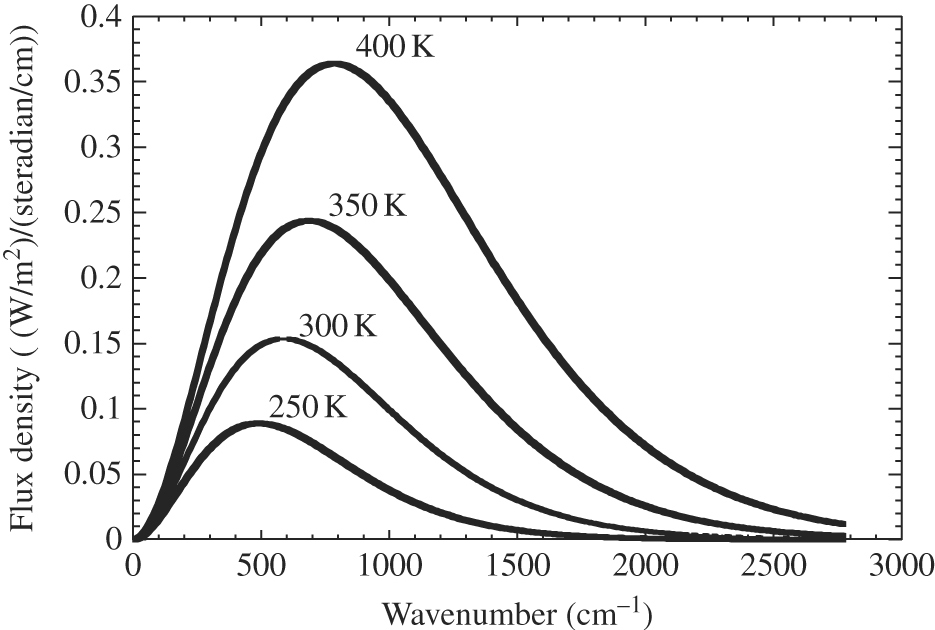
\includegraphics[width=\linewidth]{Figures/Radiative Transfer/BB Spectral Radiance.png}
        \caption{Spectral Radiance $L=B(\nu,T)$ of a Black Body}
        \label{Spec Rad BB}
    \end{subfigure}
    \begin{subfigure}{0.35\linewidth}
        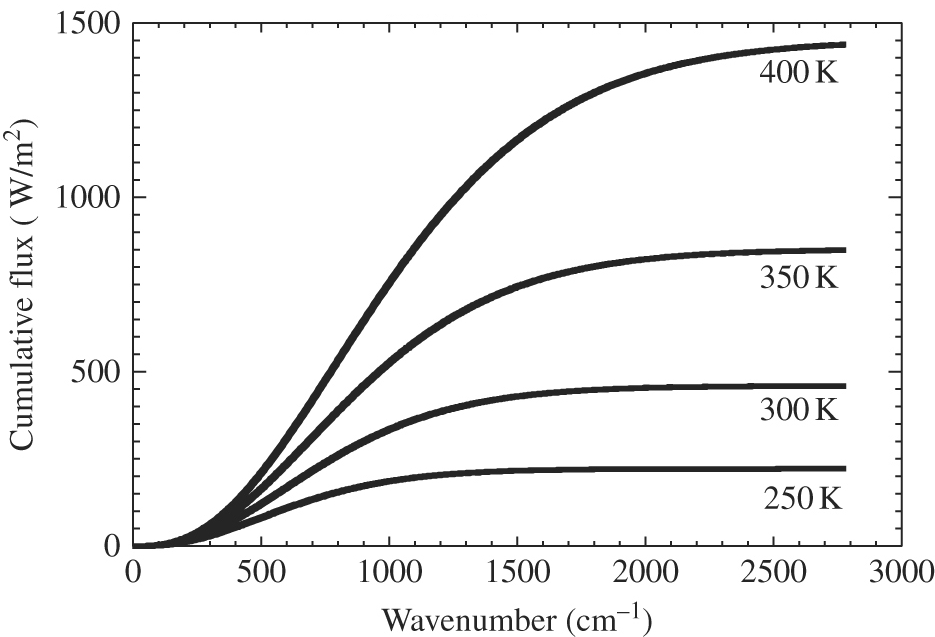
\includegraphics[width=\linewidth]{Figures/Radiative Transfer/BB Cumulative.png}
        \caption{Cumulative Radiance $\int B d\nu$ of a Black Body}
        \label{Cum BB}
    \end{subfigure}
    \begin{subfigure}{0.25\linewidth}
        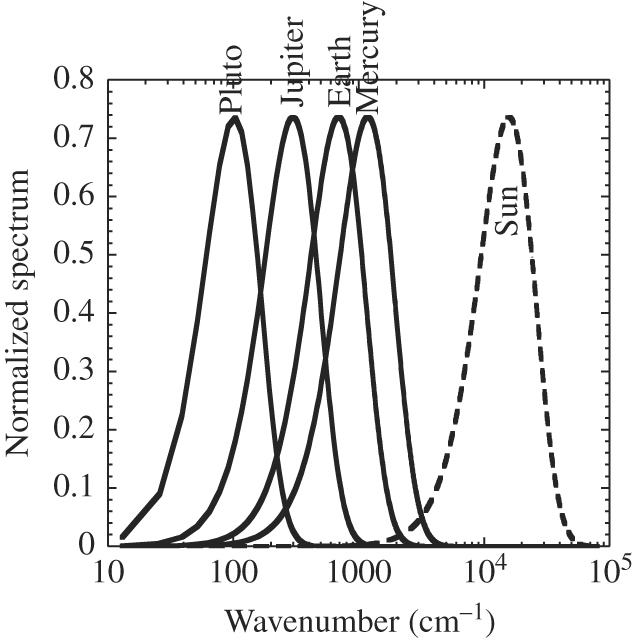
\includegraphics[width=\linewidth]{Figures/Radiative Transfer/Spectral Gap.jpg}
    \end{subfigure}
\end{figure}

Third and finally, $B$ is not a function if $\vec{\omega}$: $B$ is isotropic! This final fact allows us to calculate the spectral irradiance of a blackbody:
\begin{align*}
    F(\nu,T)&=\int_{\Omega_-} B(\nu,T)\,d\Omega_\perp\\
    &= \left( \int_{\Omega_-}d\Omega_{\perp} \right)\,B(\nu,T)\\
    &=\pi B(\nu,T)
\end{align*}

\noindent where we have set the zenith angle $\zeta$ equal to $\theta$ and integrated the projected differential solid angle:
\begin{align*}
    \int_{\Omega_-}d\Omega_\perp&=\int_{\Omega_-} \cos \zeta \,d\Omega\\
    &=\int_{0}^{2\pi}\int_{0}^{\frac{\pi}{2}} \cos \zeta \,d\theta \,\sin\theta \,d\phi\\
    &=2\pi \int_{0}^{\frac{\pi}{2}}\sin\theta\cos\theta\,d\theta\\
    &=2\pi\left[ \frac{1}{2}\sin\theta^2 \right]_0^{\frac{\pi}{2}}\\
    &=\pi
\end{align*}

To find the (non-spectral) irradiance of a black body, we integrate over all frequencies to recover the Stefan-Boltzmann Law governing the power output per unit area $P$ of a black body:
\begin{align}\label{Blackbody Frequency}
    \boxed{P=\sigma T^4=\int_0^\infty \pi B(\nu,T)\,d\nu}
\end{align}
\subsection{Emissivity and Kirchoff's Law}

Many bodies are not like blackbodies at all, even approximately. We thus define the \textbf{emissivity} $\epsilon\in[0,1]$ of an object as follows:
\begin{align}
    \BOX{\epsilon(\nu,T,p)=\frac{L(\nu,T,p)}{B(\nu,T)}}
\end{align}
where $T=$ the temperature and $p=$ the pressure of the object in question. Physically, the emissivity encodes how much the object is like a blackbody at each frequency, temperature, and pressure. For a perfect blackbody, $\epsilon=1$ for all frequencies, temperatures, and pressures. One can show that, in local thermodynamic equilibrium, the emissivity of an object is exactly equal to its absorptivity $\alpha$, where $\alpha$ is (dimensionless) the fraction of spectral radiance absorbed by the material.
\begin{align}
    \boxed{\epsilon(\nu,T,p)=\alpha(\nu,T,p)}
\end{align}

We will use this to derive the \hyperref[Schwarzschild]{Schwarzschild Equation}, which governs radiative transfer in the atmosphere. However, we should note that the derivation assumes local thermodynamic equilibrium. This is a good approximation in most parts of the atmosphere, but fails near the top of the atmosphere.

\subsection{Calulating the Stellar Constant}

To a good approximation, stellar bodies are black bodies. We can estimate the incident (not absorbed) radiative energy flux on the Earth (or any planet) from the Sun (or any star) by approximating that star as black body. The spectral radiance of the sun is approximately $B(\nu,T_{sun})$. We define the \textbf{Stellar Constant} $L_{\star}$ as the incident stellar irradiance. Note that this is different from the \textit{absorbed} stellar power – to obtain that we have to account for albedo (some incident stellar irradiance is reflected) and integrate over area. Let us now calculate $L_{\star}$. We do this by integrating the spectral radiance of the Sun over all frequencies (to obtain the radiance) and over the solid angle of the Sun from Earth (to obtain the irradiance):
\begin{align*}
    L_{\star}=\int _0^\infty \int_{\Omega_{Sun}}B_{sun}(T,\nu)\,d\Omega\,d\nu
\end{align*}

Where $\Omega_{sun}$ denotes the solid angle the sun makes from the Earth. Note that we're integrating over $d\Omega$ here, not $d\Omega_\perp$. The sun is a blackbody, and so emits isotropically, so we can simply integrate out solid angles and use the Stefan-Boltzmann Law:
\begin{align*}
    L_{\star}&=\int _0^\infty \Omega_{Sun}B_{sun}(T,\nu)\,d\nu\\
    &=\Omega_{sun}\,\sigma T_{sun}^4\frac{1}{\pi}
\end{align*}

What is the solid angle of the sun $\Omega_{sun}$ then? We can figure this out by considering a sphere centred on the Earth with a radius equal to the distance between the Earth and the Sun. The total solid angle of the entire sphere is $4\pi$, but the Sun is only occupying a small area on the surface of that sphere. The ratio of the area covered by the sun to the area of the entire sphere is $\pi R_{sun}^2:4\pi R_{Au}$, where $R_{sun}$ is the radius of the sun and $R_{Au}$ is the distance between the sun and the Earth.
\begin{align*}
    \Omega_{sun}&=4\pi\frac{\pi R_{sun}^2}{4\pi R_{Au}^2}\\
    &=\pi \frac{R_{sun}^2}{R_{Au}^2}
\end{align*}

\noindent Therefore:
\begin{align}
    L_{\star}=\frac{R_{sun}^2}{R_{Au}^2}\,\sigma T_{sun}^4
\end{align}

The power actually absorbed by the Earth is given by integrating over area and accounting for reflection. Suppose some fraction $\alpha\in[0,1]$ of the instellation is reflected. Therefore:
\begin{align*}
    P_{in}&=\int (1-\alpha)L_\star \,\cos \zeta\,dA\\
    &=(1-\alpha)L_\star\int \cos \zeta\,dA
\end{align*}

Where we have reintroduced the zenith angle factor $\cos \zeta$ (since we only integrated over $d\Omega$ before rather than $d\Omega_\perp$). This is to represent the fact that the sun is only hitting the Earth from one side, and only the component perpendicular to the ground is absorbed. As such, $\int\cos\zeta\, dA$ is the \textit{projected} area of the Earth due to the $\cos \zeta$ term, and therefore is $\pi R^2$, not $4\pi R^2$. Therefore:

\begin{align}
    P_{in} = (1-\alpha)\pi R^2 \frac{R_{sun}^2}{R_{Au}^2}\,\sigma T_{sun}^4
\end{align}

If we also approximate the Earth as a blackbody, and its radiation as isotropic, we can estimate the outgoing power:
\begin{align*}
    P_{out}&=\int\int_{\Omega_+}\int _0^\infty B(\nu,T_{Earth})\,d\nu\,d\Omega_\perp\,dA\\
    &=\left(\int dA\right)\int_{\Omega_+}\,d\Omega_\perp\int _0^\infty B(\nu,T_{Earth})\,d\nu\\
    &=(4\pi R^2)\,\sigma T_{Earth}^4
\end{align*}

From energy conservation, $P_{in}-P_{out}=0$, which we can solve for the equilibrium temperature of the Earth:
\begin{align*}
    0&=(1-\alpha)\pi R^2 \frac{R_{sun}^2}{R_{Au}^2}\,\sigma T_{sun}^4-(4\pi R^2)\,\sigma T_{Earth}^4 \\
    \therefore 0&=(1-\alpha) \frac{R_{sun}^2}{R_{Au}^2}\, T_{sun}^4-4 T_{Earth}^4 \\ 
    \therefore T_{Earth}&=T_{sun}\left(
    \frac{1-\alpha}{4}\frac{R_{sun}^2}{R_{Au}^2}
    \right)^\frac{1}{4}
\end{align*}

\section{Absorption: Optical Thickness and Transmission Function}

Suppose some spectral radiance is traveling through a slab of radiation-absorbing \textit{stuff} (e.g., air) with an infinitessimal mass-path of $d\mu$, where $d\mu$ is the mass per area (perpendicular to the propogation of radiation). We define the infinitesimal \textbf{Optical Thickness} $d\tau_\nu$ of the slab as the absorptivity $\alpha$ of the slab. In other words, suppose some spectral radiance $L$ is traveling through the radiation-absorbing \textbf{stuff}. Then the infinitesimal change of spectral radiation by the slab $dL$ is given by:
\begin{align*}
    dL &= -\alpha(\nu,T)L\\
    &= d\tau_\nu\,L
\end{align*}
where I have written $\tau_\nu$ with a subscript $\nu$ to remind us that $\tau_\nu$ is a strong function of $\nu$. We further define the absorption cross section $\kappa(\nu,T,p)$ as the effective area of spectral radiance absorbed per unit mass of absorber encountered. $\kappa$ has units of \qty{}{\metre\squared\per\kilogram}, and will generally depend on frequency, temperature, and pressure. Therefore: 
\begin{align}
    \boxed{d\tau_\nu=\kappa(\nu,T,p)\,d\mu}
    \label{Optical Thickness}
\end{align}

We can integrate this between two points in the atmosphere $p_1$ and $p_2$ to find the final spectral radiance $L_{2}$ in terms of the initial spectral radiance $L_{1}$:
\begin{align*}
    \frac{dL}{L}&=-d\tau_\nu\\
    \therefore\int_{p_1}^{p_2}\frac{dL}{L}&=-\left|\int_{p_1}^{p_2}d\tau_\nu\right|\\
    \ln\left( \frac{L_2}{L_1} \right)&=-\left|\int_{p_1}^{p_2}d\tau_\nu\right|\\
    \therefore L_2&=L_1\exp\left(-\left|\int_{p_1}^{p_2}d\tau_\nu \right|\right)
\end{align*}

Notice the absolute value in the second line. If we did not have this, we could simply reverse the limits of integration (e.g., integrate from $p_2$ to $p_1$) and obtain that the spectral radiance \textit{increases} as it passes through. However, this is clearly unphysical: the spectral radiance absorbed should be the same regardless of whether the radiation is going upwards through the absorber or downwards through the absorber. Finally, if we note that:
\begin{align*}
    \tau_\nu(p_1)-\tau_\nu(p_2)=\int_{p_1}^{p_2}d\tau_\nu=\int_{p_1}^{p_2}\kappa(\nu,T,p)\,d\mu
\end{align*}
then we can define the transmission function $\mathcal{T}_\nu$ which encodes the absorption of the spectral irradiance between those two points:
\begin{align}
    \label{Absorption}
    \mathcal{T}_\nu(p_1,p_2)=e^{-|\tau_\nu(p_1)-\tau_\nu(p_2)|}
    \\
    L_2=L_1\,\mathcal{T}_\nu(p_1,p_2)\nonumber
\end{align}

Note that it is only the transmission function which is physically and dynamically significant here, as \textit{that} is what determines absorption. We could work directly with the transmission function, but for convenience, we'd much rather work in terms of optical depth.

However, the optical depth itself is not directly physically meaningful. This is because the transmission function only cares about absolute value differences in optical depth.\footnote{
    The situation is analogous to Classical Electromagnetism or Newtonian Mechanics. In Electromagnetism and Mechanics, the only objects of physical consequence are the \textit{forces}, which depend only on the electric/magnetic fields ($\vec{E},\vec{B}$)\footnotemark and accelerations ($\ddot{\vec{r}}$) respectively. However, for convenience, we'd rather work with the electromagnetic scalar/vector potentials ($\phi,\vec{A}$) or  positions ($\vec{r}$), so we have some freedom to choose some properties of ($\phi,\vec{A}$) or ($\vec{r}$). In the former case, we must fix the gauge (e.g., pick the Lorenz or Coulomb gauge) and in the latter case, we must pick the origin and veloctiy of our coordinate system (e.g., pick the origin as the centre of the Earth). In fancy speak, we say that electromagnetism has a gauge symmetry and Newtonian mechanics has galillean symmetry. We must do a similar thing here for optical depth.
}\footnotetext{Actually the situation in electromagnetism is a bit more complicated than I've made it. In fact, only the motion of charged objects is directly observable. Since $\vec{B}$ interacts with matter through equations involve its cross product (the Biot-Savart Law and $\vec{F}=q\vec{v}\times\vec{B}$), we've used a convention of the right-handed cross product ($\vec{x}\times\vec{y}=\vec{z}$). We could have equally used the left handed cross product and had equivalent empirical predictions. I'm also not going to go into bivectors and pseudovectors here, because this footnote is already too long.} As such, we must make two choices when calculating our optical depth (analogous to choosing, e.g., the origin of our coordinate system in Newtonian mechanics):
\begin{enumerate}
    \item It's ordering: we can let $\tau_\nu$ \textit{increase} with height (decrease with pressure) or \textit{decrease} with height (increase with pressure). This is because the transmission function only cares about the absolute values.
    \item The reference value: we can pick $\tau_\nu=\tau_{\nu,ref}$ at any reference level. This is because the transmission function only cares about differences in optical depth.
\end{enumerate}
I will adopt Ray's convention here, although I should note he switches it up for convenience (as he is well within his rights to!) in section \ref{Shortwave}. As such I will choose:
\begin{enumerate}
    \item $\tau_\nu$ to increase with height, i.e., $\tau_\nu$ to decrease with pressure.
    \item $\tau_\nu$ to be equal to $0$ at the ground.
\end{enumerate}

We now specify that the spectral radiance is travelling through a slab of air with some density $\rho$ and with some absorber with mass-fraction $q$. We can see that $d\mu=q\,\rho\,dl$ where $dl$ is the length of atmosphere the radiation travels through. We further specify that the spectral radiance is traveling at some angle $\theta$ relative to the vertical so that $dl=+dz/\cos\theta$ where $z=$ the height\footnote{I could have equally chosen that $dl=-dz/\cos\theta$ here.}. Finally, we relate $dz$ to $dp$ through Hydrostatic Balance (\ref{Hydrostatic Balance}). Then:
\begin{fact}{Optical Depth Coordinates and the Transmission Function}{Optical Depth Box}\label{Optical Depth Box}
    We define the optical depth coordinate $\tau_\nu$, which encodes how much absorbing \textit{stuff} is below a pressure level $p$:

    \begin{minipage}{.5\linewidth}
        \begin{gather}
            \label{Optical Pressure}
            \BOX{d\tau_\nu=-\kappa(\nu,T(p),p)\,q(p)\frac{dp}{g\,\cos\theta}}\\
            \BOX{\tau_\nu=0\text{  at  }p=p_s}
        \end{gather}
    \end{minipage}
    \begin{minipage}{.5\linewidth}
        \begin{gather}
            \BOX{\tau_\nu(p)=\int_{p_s}^p-\kappa(\nu,T(p'),p')\,q(p')\frac{dp'}{g\,\cos\theta}}\\
            \BOX{\tau_{\nu,\infty}=\tau_\nu(0)}
        \end{gather}
    \end{minipage}
    The transmission function $\mathcal{T}_\nu$ between two points $p_1$ and $p_2$ encodes how much the spectral radiance is attenuated between the two points and is:

    \begin{minipage}{.5\linewidth}
        \begin{align}
            \BOX{
                \mathcal{T}_\nu(p_1,p_2)=e^{-|\tau_\nu(p_1)-\tau_\nu(p_2)|}
            }
        \end{align}
    \end{minipage}
    \begin{minipage}{.5\linewidth}
        \begin{align}
            \BOX{
                L(\nu,p_2)=L(\nu,p_1)\,\mathcal{T}_\nu(p_1,p_2)
            }
        \end{align}
    \end{minipage}
\end{fact}

Notice that I write $T=T(p)$ here. Until \ref{Radiative Equilibrium}, we assume that the vertical temperature profile of the atmosphere is given by some known relation (perhaps the \hyperref[Dry Adiabat]{Dry Adiabat} if we are in the troposphere).

\subsection{Example: Grey Atmosphere and Well Mixed Absorber}

Let us make three assumptions. First, assume that the atmosphere is \textit{grey}. This amounts to the assumption that the atmosphere interacts with light in the same way regardless of frequency, so $\frac{\partial\kappa}{\partial\nu}=0$. Second, assume that $\kappa$ has no $T$ or $p$ dependence. Third, assume that the absorber is \textit{well-mixed}. This means that the concentration $q$ is independent of height $\frac{\partial q}{\partial p}=0$. We can now integrate the optical depth to find:
\begin{align*}
    \tau_\nu(p)&=\int_{p_s}^p-\kappa\,q(p)\frac{dp'}{g\,\cos\theta}\\
    &=-\kappa\,q\frac{1}{g\,\cos\theta}\int_{p_s}^pdp'\\
    &=\frac{\kappa \,q}{g\,\cos\theta}(p_s-p)
\end{align*}
We define $\tau_\infty=\int_{p_s}^0d\tau_\nu$ as the optical depth of the \textit{entire} atmosphere (at that angle $\theta$). Therefore:
\begin{align*}
    \tau_\infty&=\tau(0)\\
    &=\frac{\kappa \,q}{g\,\cos\theta}(p_s-0)\\
    &=\frac{\kappa \,q\,p_s}{g\,\cos\theta}\\
    \therefore\tau_\nu(p)&=\tau_\infty\left(1-\frac{p}{p_s}\right)
\end{align*}
However, typically, $\kappa$ is a strong function of $\nu$. We will discuss how exactly $\kappa$ depends on $\nu$ in the next chapter.

\chapter{Molecular Spectroscopy}

\section{Spectral Lines}

Here we cover how the absorption cross section $\kappa$ depends on $\nu$. In almost all cases, save \hyperref[Continuum]{Continuum Absorption}, $\kappa$ is made up of many `spectral lines' (see Figure \ref{CO2 zoomed} and ignore the white lines).
\begin{figure}[H]
    \centering
    \begin{subfigure}{0.4\linewidth}
        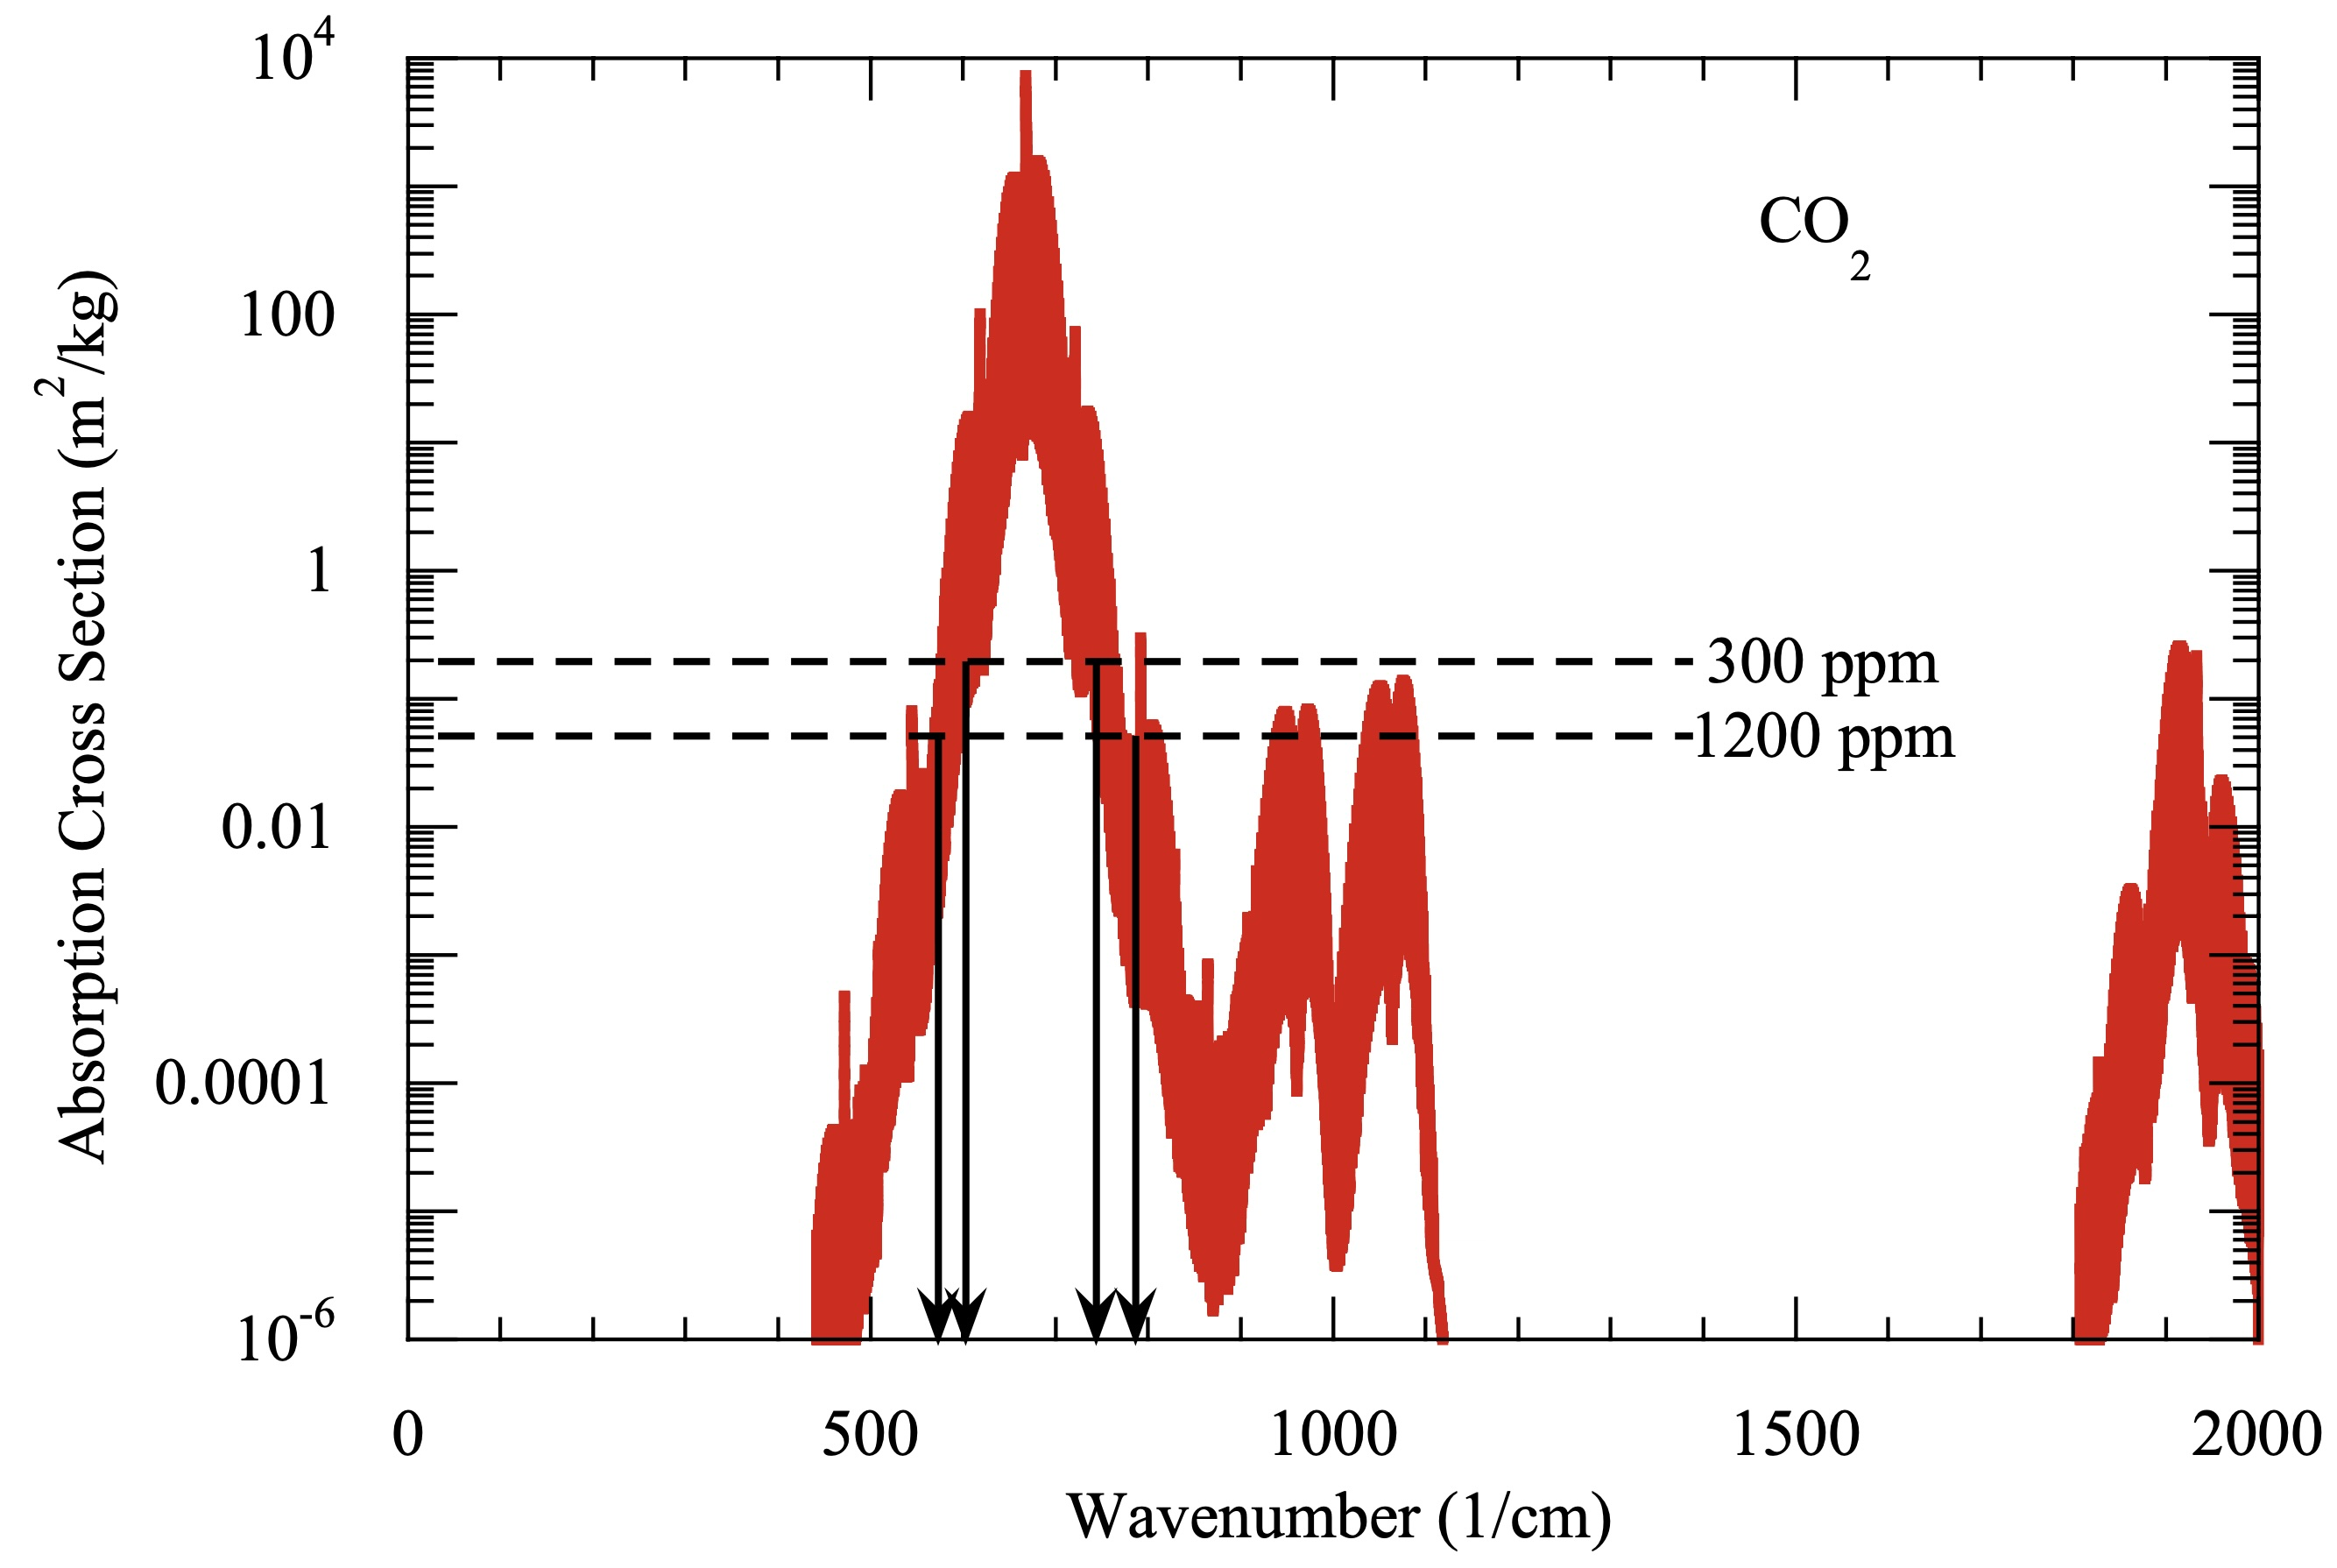
\includegraphics[width=\linewidth]{Figures/Radiative Transfer/CO2 kappa}
        \subcaption{Notice the \textbf{strong} variation over $\nu$ indicated by the logarithmic y-axis scale.}
    \end{subfigure}
    \quad
    \begin{subfigure}{0.4\linewidth}
        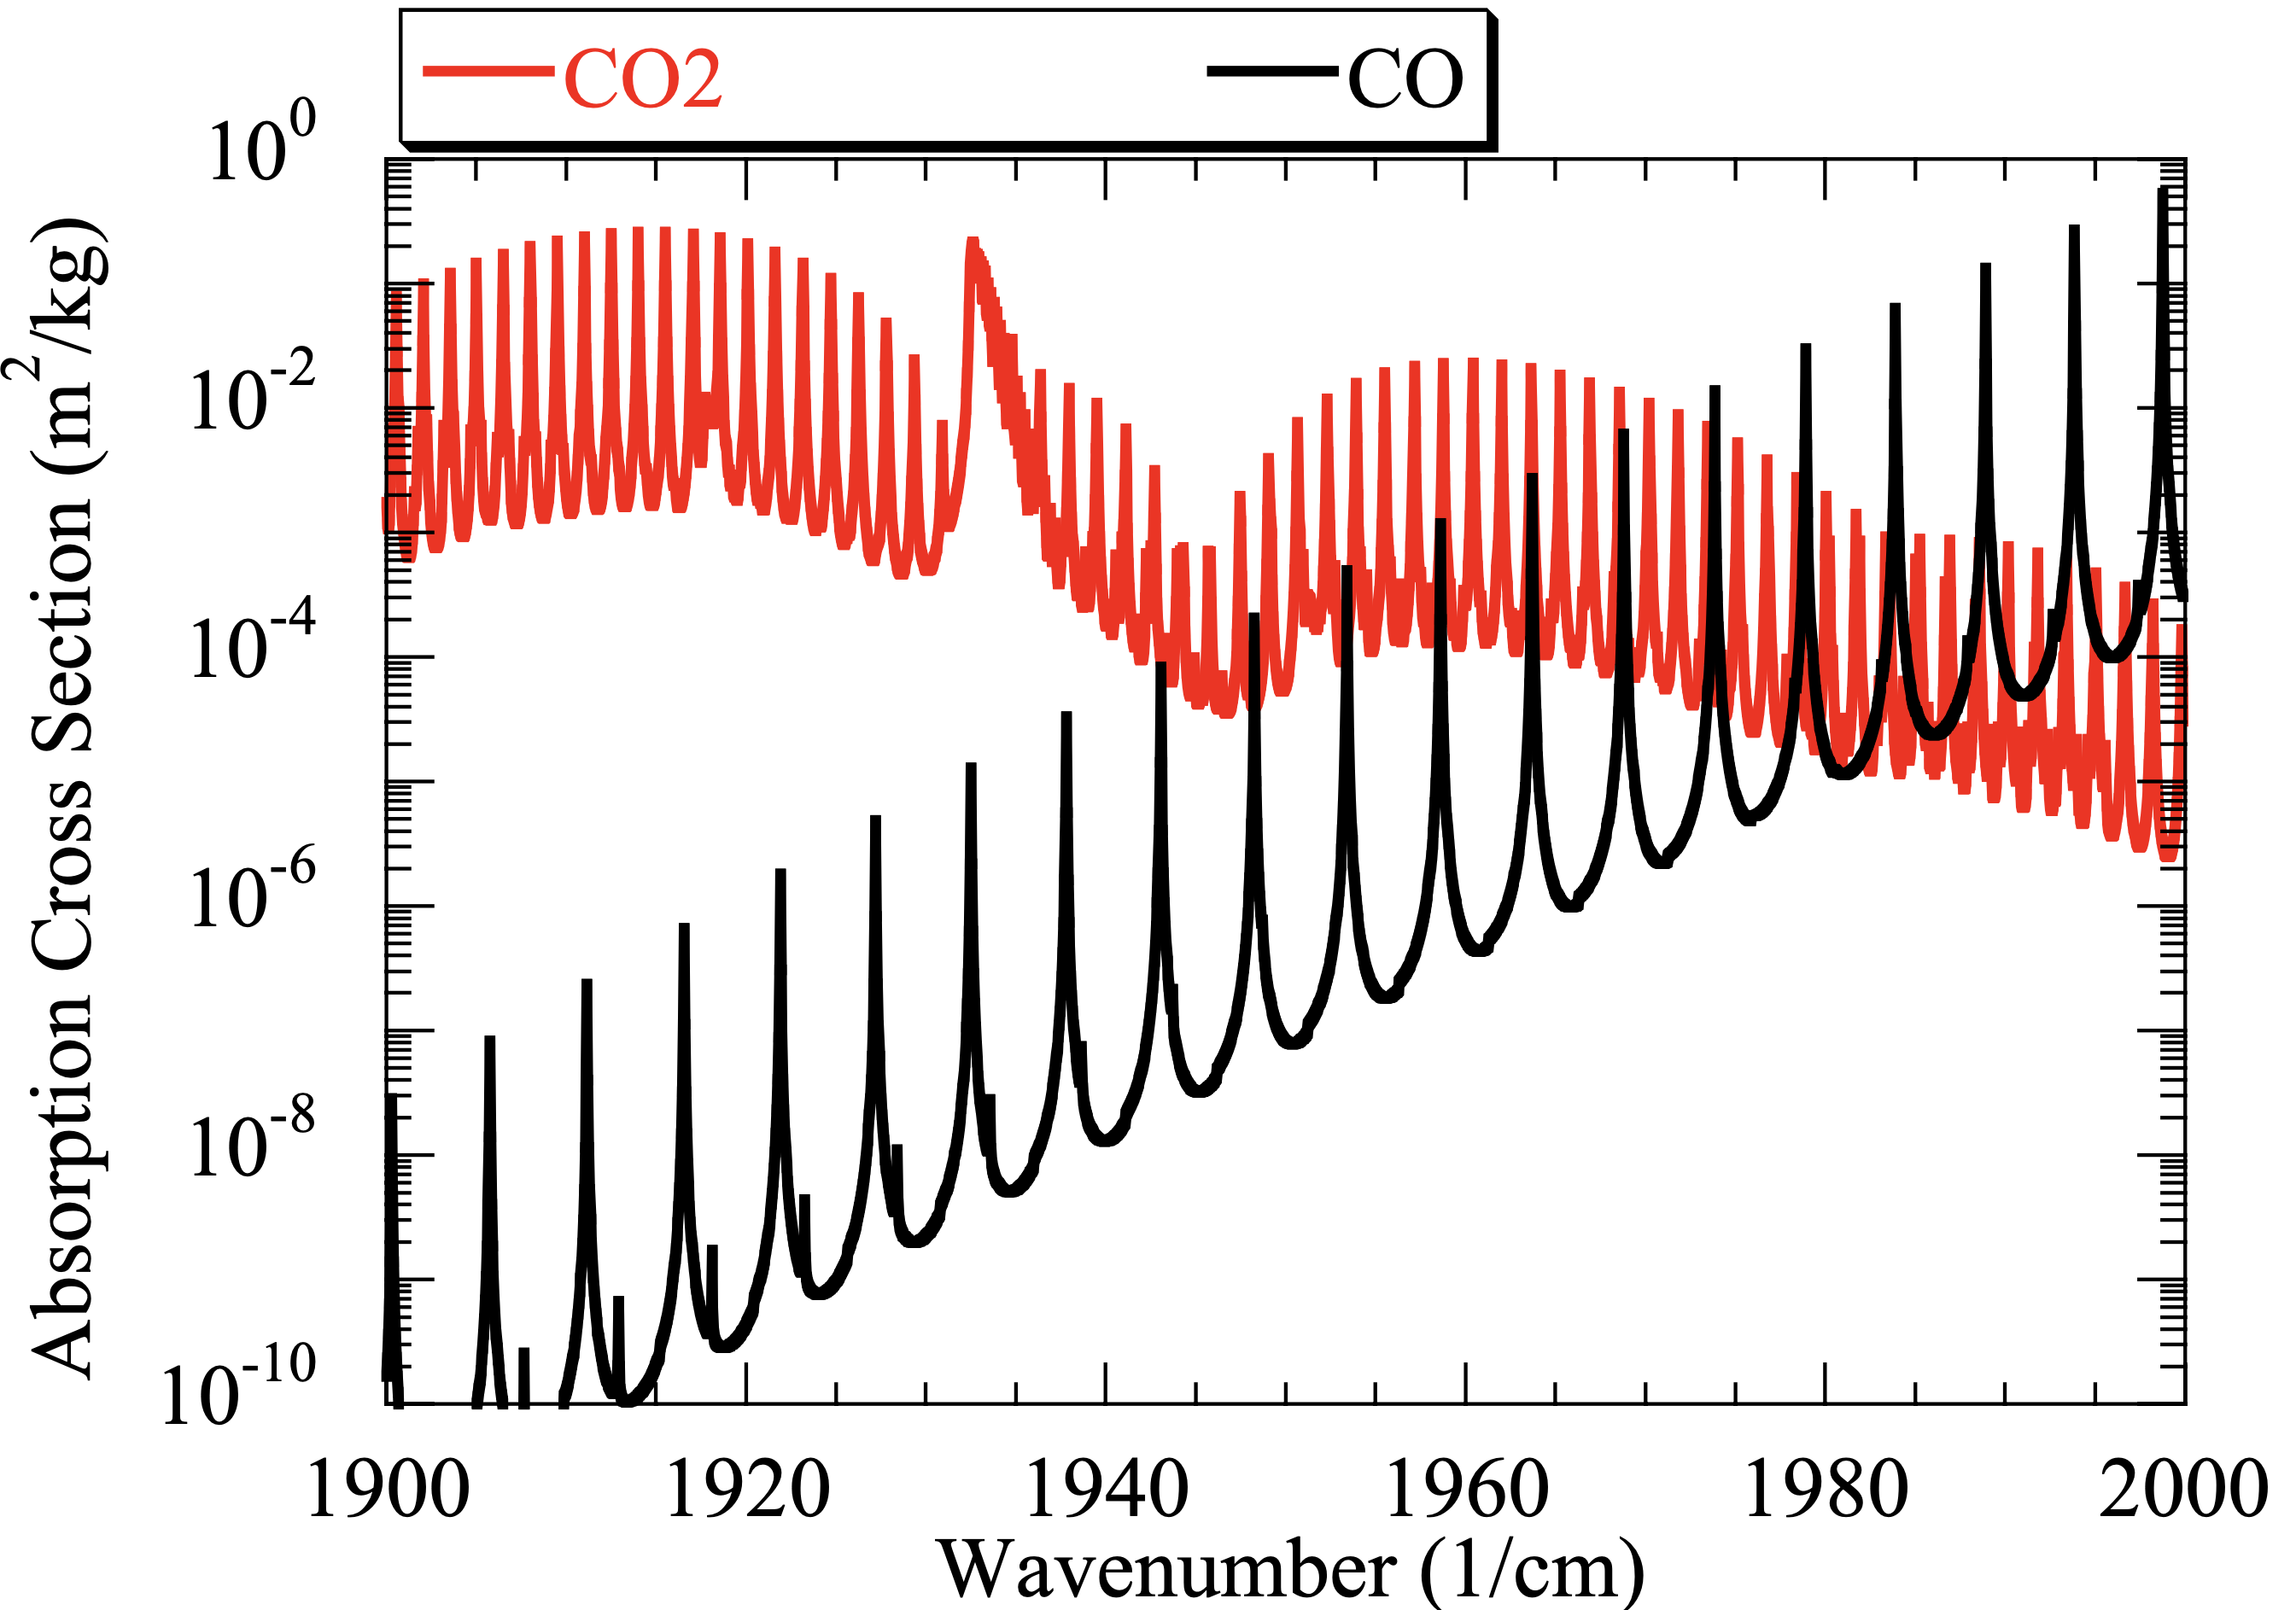
\includegraphics[width=\linewidth]{Figures/Radiative Transfer/CO2 zoomed.png}
        \subcaption{Notice how the curve is made up of \textbf{spectral lines}. }
        \label{CO2 zoomed}
    \end{subfigure}
    \caption{CO$_2$'s Absorption Cross Section at \qty{100}{\milli\bar} and \qty{260}{\kelvin}. Figures from Ray's lecture slides.}
    \label{CO2 kappa}
\end{figure}
We will discuss how to characterise the \textbf{line shape} of each individual spectral line, which we will refer to as $\kappa_{\nu_c}$: 
\begin{fact}{Line Shape}{Line Box}\label{Line Box}
    An individual spectral line is characterised as follows. All parameters have units of \qty{}{\per\second}.
    \begin{align}
        \BOX{\kappa_{\nu_c}(\nu)=\frac{S}{\delta}F\left( \frac{\nu-\nu_c}{\delta} \right)}
    \end{align}
    \begin{minipage}{.45\linewidth}
        \textbf{Line Centre} $\nu_c$:
        encodes the centre of the spectral line.

        \vspace{5 mm}
        \textbf{Line Strength} $S$: encodes how strong of an absorber the spectral line is. Defined as follows:
        \begin{align}\label{Strength}
            S=\int_{-\infty}^{\infty}\kappa(\nu)\,d\nu
        \end{align}
        Generally a function of $T$
    \end{minipage}
    \hfill
    \begin{minipage}{.45\linewidth}
        \textbf{Line Width} $\delta$:
        encodes how wide the spectral line is. Generally a function of $p$ and $T$.
        
        \vspace{5 mm}
        \textbf{Line shape} $F(x)$: encodes the shape of the line (e.g., how does the line decay as $\nu$ goes away from $\nu_c$). Normalised such that:
        \begin{align*}
            \int_{-\infty}^{\infty}F(x)\,dx=1
        \end{align*}
    \end{minipage}
\end{fact}
Why do gases absorb/emit electromagnetic radiation in the first place? Gases absorb/emit electromagnetic radiation because its consitutents, the molecules, have different states corresponding to different energy levels. If a molecule recieves just enough energy from a photon, it can transition from a lower energy level to a higher energy level, and thus absorb the photon. If a molecule is already in a higher energy level, it can spontaneously emit a photon to transition to a lower energy level.

There are three types of transitions that a molecule can undergo:
\begin{enumerate}
    \item \textbf{Electron Transitions}: An electron on the molecule hops to a higher energy state. Typically visible and UV frequency photons cause/are emitted from these transitions.
    \item \textbf{Vibrational Transitions}: The molecule begins vibrating/vibrates faster. Typically IR (Infrared) frequency photons cause/are emitted from these transitions.
    \item \textbf{Rotational Transitions}: The molecule begins rotating/rotates faster. Typically microwave frequency photons cause/are emitted from these transitions.
\end{enumerate}

We will now discuss what determines each parameter of $\nu_c$, $S$, $\delta$ and $F(x)$.

\subsection{Line Centre\texorpdfstring{ $\nu_c$}{}}

In order to discuss what determines the line centre $\nu_c$, we must discuss why spectral lines exist at all, rather than $\kappa$ having a very smooth dependence on $\nu$.

When a molecule absorbs a photon of frequency $\nu$, it must recieve energy $E=h\nu$. However, as discussed in Section \ref{Equipartition}, the energy levels of molecules are quantised, so molecules can only absorb a photon with energy equal to the energy level spacings $\Delta E$. As such, $\nu$ is constrained such that $\nu=\Delta E/h$, and this is what sets the line centre. $\Delta E$ itself is set by the quantum mechanical properties of the molecule, which is found through a variety of empirical and theoretical approaches.

A question you might (rightfully) have now is the following: if energy levels are discritised such that the molecule can only absorb energy of $E_1$, $E_2$, $E_3$, \ldots, then it can only absorb photons with a frequency \textit{exactly} equal to $\nu_1=h/E_1$, $\nu_2=h/E_2$, $\nu_3=h/E_3$, \ldots. Therefore, we should expect $\kappa$ to be a collection of infinitely thin lines, and nothing like what we see in Figure \ref{CO2 kappa}, which is a collection of thin bumps! Furthermore, since only infinitely thin lines are absorbed, then nothing is actually absorbed at all, so $\kappa=0$ for all materials! What went wrong?

This question will be answered when we discuss \hyperref[Broadening]{Broadening Mechanisms}.

\subsection{Line Strength\texorpdfstring{ $S$}{}}

The line strength $S$ is determined by two factors.

The first factor is how strongly the molecule couples with the electromagnetic field. Typically, \textbf{electron} transitions already couple strongly to the electromagnetic field, as electrons are already charged, and moving charges couple strongly to electromagnetic radiation.

For \textbf{vibrational} and \textbf{rotational} transitions, the distortions of the molecule caused by the vibrations or rotations must change the molecules electric \textbf{dipole-moment}. A full explanation of what `\textbf{dipole-moment}' means isn't possible here, but the gist of it is this: a molecule has a dipole moment if it has an uneven distribution of electric charge. For example, if it is positively charged on one end and negatively charged on the other.

H$_2$O has an intrinsic dipole moment, since the electrons in the bonds are more closely bound to the oxygen, and so the oxygen is a little bit negatively charged and the hydrogens are a little bit positively charged. Vibrations and rotations alter this, and this makes H$_2$O a very strong infrared absorber.

CO$_2$ has no intrinsic dipole moment, but it has two vibrational modes (INSERT FIGURE HERE) which alter its dipole moment. This is typical of linear triatomic molecules. As such, it is a strong infrared absorber as well.

Meanwhile, N$_2$ and O$_2$ are both diatomic molecules made up of identical atoms, and so don't couple strongly to the electromagnetic field, since none of the rotational or vibrational modes change the molecules' dipole moment. This is why N$_2$ and O$_2$ are both optically inactive.

The second factor depends on the average occupation of the energy states. The intuition is as follows. Suppose a spectral line has a line centre at $\nu_c$, and thus relies on a transition from energy levels from $E_i$ to $E_j$ (such that $E_j-E_i=h\nu_c$). A gas that has, say, half of its molecules in energy state $E_j$ will have half of its molecules able to absorb a molecule of frequency $\nu_c$, but a gas that has a higher proportion (say, three-quarters) will have a higher proportion of its molecules (say, three-quarters) able to absorb a molecule of frequency $\nu_c$.

The occupation of energy states depends on the temperature of a system, and one can derive this using statistical mechanics. We won't derive it here, but the result for the functional form of $S$ for IR (Infra-red) radiation is as follows:
\begin{align*}
    S(T)=S(T_0)\frac{Q(T_0)}{Q(T)}\left( 
        \frac{1-\exp\left( \frac{-h\nu_c}{k_BT} \right)}{1-\exp\left( \frac{-h\nu_c}{k_BT_0} \right)}\exp\left( 
            -\frac{h\nu_l}{k_B}\left( \frac{1}{T}-\frac{1}{T_0} \right)
         \right)
     \right)
\end{align*}
where $h\nu_l$ is the energy of the lower energy state and $Q(T)$ is some function of $T$ depending on the molecule. You do not need to memorise or understand much of this equation, but it's important to note that the main dependence comes from the exponential terms. $S$ \textbf{strongly} increases with temperature (it has an exponential dependence): as temperature increases, line-strength also increases.

\section{Broadening Mechanisms: Line Shape\texorpdfstring{ $F$}{} and Width\texorpdfstring{ $\delta$}{}}\label{Broadening}

If we stop our discussion here, then we would have a collection of infinitely thin lines,and so $F(x)=\delta(x)$ for all lines, where $\delta$ is the dirac delta function. However, lines are clearly \textbf{broadened} (see Figure \ref{CO2 zoomed}) and are not delta functions. There are three physical mechanisms which explain why lines are broadened in our context, and why molecules may absorb/emit photons with frequency $\nu$ close to $\nu_c$ but not equal to $\nu_c$.

\subsection{Uncertainty Broadening}

One can show, but we won't show it here, that the following relation holds:
\begin{align*}
    Var(\hat{E})\,\tau=h/2
\end{align*}
where $Var(\hat{E})$ is the variance of the energy of the system, $\tau$ is the expected lifetime of the system, and $h$ is Planck's constant. To be perfectly honest, I do not fully understand how this equation arises, and what relation this bears to the Heisenberg Uncertainty Relation other than a superficial resemblance.\footnote{
    The Heisenberg Uncertainty Relation relates the variance in momentum and variance in position of any quantum system. Despite what I see as a superficial resemblance, I will be using the name `Uncertainty Broadening' because that's what it's called in C5 and I don't want to confuse you. If I could choose though, I'd probably use the sometimes-used `Lifetime Broadening' or `Natural Broadening'.
}

Let's now interpret the consequences of the equation on the molecules we're considering. The lifetime of a system $\tau$ encodes how stable the system is. Recall that a molecule is in an `excited' state before emitting a photon or after absorbing a photon. This state is, generally, meta-stable, and thus has a finite lifetime ($\tau\neq\infty$) after which it has a high probability of emitting a photon and transitioning to a lower energy state.

The variance of the energy $Var(\hat{E})$ represents the fact that, because of this, these molecules aren't actually in a state of exact/definite energy (called an energy eigenstate). This means that when a system transitions from one energy state to another energy state, the energy difference can actually be approximately equal to $\Delta E$, with some spread determined by the lifetime of the system $\tau$.

One can determine the line width and shape from these principles more rigourously, but it turns out that in normal atmospheric circumstances this line width is negligible, so we do not discuss this in C5. It will suffice for you simply to know that, regardless of whether the upcoming two broadening mechanisms come into effect, there is some natural Uncertainty Broadening mechanism which ensures that \textit{all} lines have finite width.

\subsection{Doppler Broadening}

Our second broadening mechanism is doppler broadening, and this occurs because the molecules in the gas might be moving away/towards us when they absorb or emit a photon. As such, the photon will be red or blue shifted.

Since the molecules are moving at non-relativistic speeds, the (doppler-shifted) frequency $\nu$ we see is related to the actual linecentre $\nu_c$ by:
\begin{align*}
    \nu=\nu_c+(1+v/c)
\end{align*}
where $c=$ the speed of light and $v=$ the velocity the particle is moving in towards/away us.

The actual line-width is thus fixed by the velocity distribution of the molecules. This is predicted by the Maxwell-Boltzmann Distribution using Kinetic Theory, and so we get that:
\begin{gather}
    \label{Doppler Broadening F}
    \boxed{
        F(x)=\frac{1}{\sqrt{\pi}}e^{-x^2}
    }\\
    \label{Doppler Broadening delt}
    \boxed{
        \delta(T) = \frac{\nu_c}{c}\left( \frac{2k_BT}{m} \right)^{\frac{1}{2}}
    }
\end{gather}
So the line-width is scales as $\sqrt{T}$ – the line gets thicker as the gas gets hotter. Conversely, if the temperature falls to $0$ this equation predicts that the line width would fall to $0$, and so $\kappa(\nu=\nu_c)\to\infty$. However, this never happens, as Uncertainty Broadening maintains a non-zero line width.

This is mechanism of broadening is much more substantial than Uncertainty Broadening, but it is still very thin for two reasons. First, as seen from \ref{Doppler Broadening F}, the line shape is exponential in $x$. As such, $F$ falls off extremley rapidly as $\nu$ moves away from $\nu_c$. Second, as seen from \ref{Doppler Broadening delt}, generally $\delta\ll\nu_c$ since $\left( \frac{2k_BT}{m} \right)^{\frac{1}{2}}\ll c$\footnote{Physically, $\left( \frac{2k_BT}{m} \right)^{\frac{1}{2}}$ is proportional to the mean speed of the molecules.}. However, it is dominant in the stratosphere.

\subsection{Collisional/Pressure Broadening}

In the troposphere, this is by far the most important type of broadening. This arises because the kinetic energy of a molecule is not actually quantised. As such, if a molecule is colliding with another molecule while a photon hits it, it can borrow/give some energy to the other molecule to absorb a photon of slightly different frequency than $\nu_c$.

The broadening thus scales with the frequency of collisions, which depends on the pressure and temperature. This gives us the Lorentz Profile:
\begin{fact}{Lorentz Line Shape}{Lorentz Box}\label{Lorentz Box}
    The shape $F$ and width $\delta$ of a spectral line is, in planetary climate contexts, mainly set by the Lorentz Line shape: 
    \begin{multicols}{2}
    \begin{align}
        \label{Lorenz F}
        \BOX{F(x)=\frac{1}{\pi}\frac{1}{x^2+1}}
    \end{align}

    \vspace{18 mm}
    \begin{align}
        \label{Lorenz width}
        \BOX{
            \delta \approx \delta_0\,\frac{p}{p_0}\left( \frac{T_0}{T} \right)^{n}
        }
    \end{align}
    \end{multicols}
    where $\delta_0$, $p_0$, $T_0$ are all reference widths, pressures, and temperatures and $n$ is a dimensionless constant. All constants are, in practice, found empirically. Oftentimes, $n\approx 1/2$.
\end{fact}
As we can see then, pressure broadening results in pressure \textit{increasing} the line width and temperature \textit{decreasing} the line width. If, for example, the pressure were to fall to $0$ this equation predicts that the line width would fall to $0$, and so $\kappa(\nu=\nu_c)\to\infty$. However, again, this never happens, as Uncertainty Broadening (and Doppler Broadening if $T\neq 0$) would maintain a non-zero line width.

You should memorise this for the exam Key Idea \ref{Lorentz Box} for the exam.

\section{Continuum Absorption}\label{Continuum}

[Under Construction]

\chapter{The Schwarzschild Equation}

\section{The Equations of Motion}

Consider some radiation traveling through a slab of atmosphere at some zenith angle $\theta$ with some spectral radiance $L$ with some frequency $\nu$. We wish to derive how $L(\nu)$ varies as it propogates through the atmosphere. Suppose the slab of atmosphere has vertical infintesimal optical thickness of $d\tau_\nu^*$. Since the path of the radiation is slanted, the spectral radiance travels through an infinitesimal optical depth of $d\tau_\nu=d\tau_\nu^*/\cos\theta$. The slab absorbs some spectral radiance, but it also emits some spectral radiance:

\begin{figure}[H]
    \centering
    \begin{tikzpicture}
        \draw[-] (1,0) -- (14,0) -- (14,1) -- (1,1) -- (1,0);
        \draw[<->] (14.5,0) -- (14.5,1);
        \node[] at (16,0.5) {$d\tau_\nu^*=d\tau_\nu\cos\theta$};
        \draw[->,ultra thick] (13,-1) -- (9,0);
        \draw[->,ultra thick,dashed] (9,0) -- (5,1);
        \draw[-] (9,0) -- (9,1);
        \coordinate (C) at (9,1);
        \coordinate (A) at (9,0);
        \coordinate (B) at (5,1);
        \draw (C) -- (A) -- (B)
            pic [draw=black, fill=myorange,angle radius=4mm, opacity=0.5] {angle = C--A--B};
        \draw[<->] (7,0) -- (3,1);
        \node[] at (4,0.5) {$d\tau_\nu$};
        \draw[->,ultra thick] (5,1) -- (1,2);
        \draw[->, ultra thick] (13,1) -- (9,2);
        \node[] at (11.25,1.75) {$B\,d\tau_\nu$}; 
        \node[] at (6,1.75) {$L(\tau_\nu^*)-L(\tau_\nu^*)\,d\tau_\nu$};
        \node[] at (10.75,-0.75) {$L(\tau_\nu^*)$};
        \node[] at (8.5,0.5) {$\theta$};
    \end{tikzpicture}
\end{figure}

The spectral radiance going into the slab is $L(\tau_\nu^*)$. The spectral radiance going out of the slab is $L(\tau_\nu^*+d\tau_\nu^*)$, which we wish to express in terms of $L(\tau_\nu^*)$. We know that some proportion $\alpha$ of $L(\tau_\nu^*)$ is absorbed by the radiation and that this proportion is equal to the absorptivity $\alpha(\nu,T) = d\tau_\nu$. However, we also know that the slab of atmosphere also emits radiation equal to $\epsilon(\nu,T)\,B(\tau_\nu^*)$, where $\epsilon=$ the emissivity. Therefore:
\begin{align*}
    L(\tau_\nu^*+d\tau_\nu^*)&=L(\tau_\nu^*)\underbrace{(1-\alpha)}_{\text{absorption}}+\underbrace{\epsilon B(\tau_\nu^*)}_\text{emission}\\
    &=L(\tau_\nu^*) - L(\tau_\nu^*)\,d\tau_\nu + \epsilon B(\tau_\nu^*)
\end{align*}
We now assume that the slab is in local thermodynamic equilibrium, and so $\epsilon=\alpha=d\tau_\nu$ and rearrange to get:
\begin{align*}
    \frac{L(\tau_\nu^*+d\tau_\nu^*)-L(\tau_\nu^*)}{d\tau_\nu}=-L(\tau_\nu^*)+B(\tau_\nu^*)
\end{align*}
Inconveniently, our coordinate $d\tau_\nu$ depends on $\theta$, but we wish to have a coordinate be the same at every horizontal position. We thus define $d\tau_\nu^*=d\tau_\nu\cos\theta$ and derive the \textbf{Schwarszchild Equation}:
\begin{align}\label{Schwarzschild}
    \BOX{
        \cos(\theta)\frac{dL}{d\tau_\nu^*}(\tau_\nu^*)=-L(\tau_\nu^*)+B(\nu,T(\tau_\nu^*))
    }
\end{align}

\section{Angle Averaging: The Two-Stream Approximation}\label{Two Stream Approximation}

Note that generally, $L$ is a function of direction ($\frac{\partial L}{\partial \vec{\omega}}\neq0$). We proceed by making what's called the \textit{Two-Stream Approximation}, but we need not make this approximation if we were coding up a full radiative transfer model. We only assume this here to make analytical progress in order to gain some physical intuition.

We define the net upwards and downward fluxes of irradiance as follows:
\begin{align}
    F_+&=\int_{\Omega_+}L(\vec{\omega})\,d\Omega_\perp \\
    F_-&=-\int_{\Omega_-}L(\vec{\omega})\,d\Omega_\perp 
\end{align}

Note that Ray refers to these as $I_+$ and $I_-$ in his notes. However, we shall refer to them here by the letter $F$, because these are (spectral) \textbf{irradiances}, \textbf{not} (spectral) \textbf{radiances}, as we have integrated over solid angles here. We then integrate Equation \ref{Schwarzschild} in the upwards and downwards directions, and make the assumption that $B$ is isotropic.
\begin{align*}
    \int_{\Omega_+}\cos(\theta)\frac{dL}{d\tau_\nu^*}\,d\Omega&=\int_{\Omega_+}-L+B\,d\Omega\\
    \int_{\Omega_+}\frac{dL}{d\tau_\nu^*}\,d\Omega_\perp&=-\int_{\Omega_+}L\,d\Omega+\int_{\Omega_+}B\,d\Omega\\
    \frac{dF_+}{d\tau_\nu^*}&=-\int_{\Omega_+}L\,d\Omega+2\pi B
\end{align*}

So far, everything is roughly very accurate. We now make the \textit{Two-Stream Approximation} in order to relate $F_+$ to $\int_{\Omega_+}L\,d\Omega$. We make (counter-intuitively) the assumption that $L(\vec{\omega})$ is roughly isotropic enough to be pulled outside of the integral over solid angle. This allows us to find that:
\begin{align*}
    \int_{\Omega_+}L\,d\Omega&\approx L\int_{\Omega_+}\,d\Omega \\
    & = L\,2\pi \\
    & = 2\pi \,L \frac{\int_{\Omega_+}\,d\Omega_\perp}{\int_{\Omega_+}\,d\Omega_\perp} \\
    & \approx 2\pi \frac{\int_{\Omega_+}L\,d\Omega_\perp}{\int_{\Omega_+}\,d\Omega_\perp} \\
    & = 2\pi \, \frac{F_+}{\pi}\\\int_{\Omega_+}L\,d\Omega & \approx 2F_+
\end{align*}
We can go through a similar reasoning with $F_-$, which allows us to derive the angle-averaged upwards and downwards Schwarszchild Equations:
\begin{align}
    \label{Upwards Schwarszchild Initial}
    {\frac{1}{2}\frac{dF_+}{d\tau_\nu^*}=-F_++\pi B}\\
    \label{Downwards Schwarszchild Initial}
    {-\frac{1}{2}\frac{dF_-}{d\tau_\nu^*}=-F_-+\pi B}
\end{align}

Note the extra `$-$' sign on Equation \ref{Downwards Schwarszchild Initial}. Comparing \ref{Upwards Schwarszchild Initial} with \ref{Schwarzschild}, we can conclude that this approximation is equivalent to setting $\cos(\theta)=\frac{1}{2}$ on average! With this in mind, we define the effective propagation angle $\tilde{\theta}$ as $\tilde{\theta}=\cos^{-1}(1/2)$. We now abuse notation and define $\tau_\nu\equiv \tau_\nu^*/\cos(\tilde{\theta})=2\tau_\nu^*$ to get rid of that pesky $\frac{1}{2}$ factor to obtain the: 
\begin{fact}{Angle-Averaged Schwarzschild Equations}{Schwarz box}\label{Scharz box}
    The following equations govern the net upward ($F_+$) and downwards ($F_-$) spectral irradiance, derived from the \hyperref[Schwarzschild]{Schwarszchild Equation} using the \textit{Two-Stream Approximation}.

    \begin{minipage}{.5\linewidth}
        \begin{gather}
        \label{Upwards Schwarzschild}
        \BOX{\frac{dF_+}{d\tau_\nu}(\tau_\nu)=-F_+(\tau_\nu)+\pi B}
        \end{gather}
    \end{minipage}
    \begin{minipage}{.5\linewidth}
        \begin{gather}
        \label{Downwards Schwarzschild}
        \BOX{-\frac{dF_-}{d\tau_\nu}(\tau_\nu)=-F_-(\tau_\nu)+\pi B}
        \end{gather}
    \end{minipage}

    We can relate optical depth coordinates $\tau_\nu$ to pressure coordinates $p$ using \ref{Optical Pressure}:
    \begin{align}
        d\tau_\nu&=-\kappa(\nu,T(p),p)\,q(p)\frac{dp}{g\frac{1}{2}}\\
        &=-\kappa(\nu,T(p),p)\,q(p)\frac{dp}{g\cos\tilde{\theta}}
    \end{align}
    where $\tilde{\theta}=$ the effective propagation angle.
\end{fact}


\section{General Solutions and Radiating Level}

We can integrate \ref{Upwards Schwarzschild} and \ref{Downwards Schwarzschild} using an integrating factor and a single boundary condition to find:
\begin{align}
    \BOX{F_+(\nu,\tau_\nu)=F_+(\nu,0)e^{-\tau_\nu}+\int_0^{\tau_\nu}\pi B(\nu,T(\tau_\nu'))e^{-(\tau_\nu-\tau_\nu')}\,d\tau_\nu'} \label{Upwards Soln}\\ 
    \BOX{F_-(\nu,\tau_\nu)=F_-(\nu,\tau_{\nu,\infty})e^{-(\tau_{\nu,\infty}-\tau_\nu)}+\int_{\tau_\nu}^{\tau_{\nu,\infty}}\pi B(\nu,T(\tau_\nu'))e^{-(\tau_\nu'-\tau_\nu)}\,d\tau_\nu'} \label{Downwards Soln}
\end{align}
where we have used the boundary conditions:
\begin{align*}
    \text{at the ground }\boxed{\tau_\nu=0\text{ , } F_+(\nu,\tau_\nu)=F_+(\nu,0)}\\
    \text{at the top fo the atmosphere }\boxed{\tau_\nu=\tau_{\nu_\infty}\text{ , } F_-(\nu,\tau_\nu)=F_-(\nu,\tau_{\infty})}
\end{align*}

There are three subtleties we should note. First, note the sign flips between \ref{Upwards Soln} and \ref{Downwards Soln}, arising due to the sign flip on the derivative in \ref{Upwards Schwarzschild} and \ref{Downwards Schwarzschild}. Second, note that the limits of integration are swapped between \ref{Upwards Soln} and \ref{Downwards Soln}, arising due to the difference in boundary conditions.

The final subtlety is the most important: in general $\tau_\nu=\tau_\nu(\nu)$. Suppose we wish to the total radiative upwards flux of energy at some height/pressure level. We cannot simply find $F_+(\tau=\tau(p))$ then integrate over all frequencies, as in general $\tau_{\nu_1}(p)\neq\tau_{\nu_2}(p)$.

Physically, the solution is intuitive: the total upwards radiance at some optical depth $\tau$ is simply the sum of the irradiance at each level $\tau'$, each attenuated by the transmission function between $\tau$ and $\tau'$. To be more explicit, we sum:
\begin{enumerate}
    \item $F_+(\nu,0)e^{-\tau_\nu}$: The irradiance ($F_+(\nu,0)$) from the bottom ($\tau_\nu=0$) of the atmosphere, attenuated by the optical depth $e^{-(\tau_\nu-0)}$.\footnote{Generally, this is the upwards irradiance emitted by the ground on a rocky planet, but one could also choose $\tau_\nu=0$ in the middle of the atmosphere (as you must on a gaseous planet), in which case $F_+(\nu,0)$ will be the total upwards irradiance at that level (originating from all the atmosphere (and ground) underneath it).}
    \item $\pi B(\nu,T(\tau_\nu'))\,d\tau_\nu'\,e^{-(\tau_\nu-\tau_\nu')}$: The irradiance ($B(\nu,T(\tau_\nu'))\,d\tau_\nu'$) from each layer ($\tau_\nu=\tau_\nu'$), also attenuated by the optical depth $e^{-(\tau_\nu-\tau_\nu')}$
\end{enumerate}
The \textbf{Outgoing Longwave Radiation} $OLR$ (in spectral irradiances) is then defined as $F_+(\nu,p=0)=F_+(\nu,\tau=\tau_{\nu,\infty})$ and given by:
\begin{align}
    \BOX{OLR=F_+(\nu,0)e^{-\tau_{\nu,\infty}}+\int_0^{\tau_{\nu,\infty}}\pi B(\nu,T(\tau_\nu'))e^{-(\tau_{\nu,\infty}-\tau_\nu')}\,d\tau_\nu'} \label{OLR Soln}
\end{align}
The physical interpretation is identical. The total upwards spectral irradiance escaping is the spectral irradiance from each level attenuated by the amount of absorption in between those levels.

Since the attenuation is exponential, this gives us an optical depth `lengthscale' set by when $(\tau_{\nu,\infty}-\tau_\nu')\sim 1$. This allows us to define:
\begin{fact}{The Radiating Level $p_{rad}$}{rad level box}\label{rad level box}
    We define the \textbf{radiating level} at $\tau_\nu=\tau_{\nu,rad}$ and $p=p_{rad}$ which satisfy the following relations:

    \begin{minipage}{.5\linewidth}
    \begin{align}
        \BOX{\tau_{\nu,\infty}-\tau_{\nu,rad} = 1}\\
        \BOX{\tau_\nu(p_{rad})=\tau_{\nu,rad}}
    \end{align}
    \end{minipage}
    \begin{minipage}{.5\linewidth}
        Figure here!
    \end{minipage}

    Physically, the interpretation is as follows: any radiation coming from an optical depth $\tau_\nu<\tau_{\nu,rad}$ ($p>p_{rad}$) will be attenuated \textbf{much} more than radiation coming from an optical depth $\tau_\nu>\tau_{\nu,rad}$ ($p<p_{rad}$).

    As such, the $OLR$ radiation actually escaping into space will disproportionately look like the radiation emitted by `stuff' at $p_{rad}$. In other words, if you were to look down at the atmosphere, you would not `see' anything from an optical depth coming from $p>p_{rad}$. 
\end{fact}
Note that this definition only really works if $\tau_{\nu,\infty}>1$. If $\nu$ is in the visible light region, for example, $\tau_{\nu,\infty}<0$, which is why you can see all the way to the ground (since $p_{rad}=p_s$, since $\tau_\nu\to-\infty$ at the ground due to the discontinuity of switching between something optically thin (the atmosphere) and something optically thick (the ground)).

We can also express everything in terms of the transmission function. Defining the radiating level in terms of the transmission function is straightforward: $p_{rad}$ satisfies the following relation\footnote{And, of course, $p_{rad}>0$.}:
\begin{align}
    \mathcal{T}_\nu(0,p_{rad})=e^{-1}
\end{align}
We can also rewrite \ref{Upwards Schwarszchild Initial} and \ref{Downwards Schwarszchild Initial} in terms of the transmission function $\mathcal{T}_\nu(p_1,p_2)$ if we find the differential of the transmission function with respect to $p_2$ and assume that $\tau_\nu(p_1)\geq\tau_\nu(p_2)$ (i.e., if $p_1\leq p_2$):
\begin{align*}
    d\left( \mathcal{T}_\nu(p_1,p_2) \right)&=d\left( e^{-|\tau_\nu(p_1)-\tau_\nu(p_2)|} \right)\\
    &=e^{-\tau_\nu(p_1)} d\left(e^{\tau_\nu(p_2)} \right)\\
    &= e^{-\tau_\nu(p_1)}e^{\tau_\nu(p_2)}d\tau_\nu(p_2) \\
    &=e^{-|\tau_\nu(p_1)-\tau_\nu(p_2)|}d\tau_\nu(p_2)\\
    \therefore\,\,d\mathcal{T}_\nu(p_1,p_2)&=\mathcal{T}_\nu(p_1,p_2)\,d\tau_\nu(p_2)
\end{align*}
If, conversely, $\tau_\nu(p_1)\leq\tau_\nu(p_2)$ (i.e., if $p_1\geq p_2$), then $d\mathcal{T}_\nu(p_1,p_2)=-\mathcal{T}_\nu(p_1,p_2)\,d\tau_\nu(p_2)$.

\begin{fact}{Solution to the Angle-Averaged Schwarszchild Equations}{Soln Schwarszchild Box}\label{Soln Schwarszchild Box}
    The total upwards $F_+(\nu,p)$ and downwards $F_-(\nu,p)$ spectral irradiance at frequency $\nu$ and pressure level $p$ is given by the following:
    \begin{gather}
        \label{Upwards Transmission Soln}
        \BOX{F_+(\nu,p)
        =
        F_+(\nu,0)\mathcal{T}_\nu(p,p_s)
        +
        \int_{p'=p_s}^{p}\pi B(\nu,T(p'))\,d\mathcal{T}_\nu(p,p')} 
        \\ 
        \label{Downwards Transmission Soln}
        \BOX{F_-(\nu,p)
        =
        F_-(\nu,0)\mathcal{T}_\nu(0,p)
        -
        \int_{p'=p}^{0}\pi B(\nu,T(p'))\,d\mathcal{T}_\nu(p,p') }
    \end{gather}
    where $d\mathcal{T}_\nu(p,p')$ is the differential transmission function with respect to $p'$. $d\mathcal{T}_\nu(p,p')=\mathcal{T}_\nu(p,p')\,d\tau_\nu(p')$ if $p\leq p'$ (as in \ref{Upwards Transmission Soln}) or $d\mathcal{T}_\nu(p,p')=-\mathcal{T}_\nu(p,p')\,d\tau_\nu(p')$ if $p\geq p'$ (as in \ref{Downwards Transmission Soln}).

    The \textbf{Outgoing Longwave Radiation} $OLR$ (in spectral irradiances) is then defined as $F_+(\nu,p=0)=F_+(\nu,\tau=\tau_{\nu,\infty})$ and given by:
    \begin{align}
        \BOX{OLR=
        F_+(\nu,0)\mathcal{T}_\nu(0,p_s)
        +
        \int_{p_s}^{0}\pi B(\nu,T(p'))\,d\mathcal{T}_\nu(0,p') }\label{OLR Transmission Soln}
    \end{align} 
\end{fact}

Note that even though the integral in \ref{Upwards Transmission Soln} is taken from $p$ to $p<p_s$, the integral is positive because $d\mathcal{T}_\nu(p,p')<0$, because $d\mathcal{T}_\nu(p,p')\sim d\tau(p')\sim - dp'$.

\section{Frequency Bands}\label{Frequency Bands}

We're not finished yet! Recall that we have expressed $OLR$ in terms of \textit{spectral} irradiances, but we require the (non-spectral) irradiances if we wish to compute the total outgoing radiative energy flux. What we may do now is integrate the $OLR$ over the centre of a single absorption band centred about $\nu_c$. Typically, both $F_+(\nu,0)$ and $B(\nu,T)$ are roughly constant as a function of $\nu$ compared to $\tau_\nu$, so we can treat $F_+(\nu,0)\approx F_+(\nu_c,0)$ and $B(\nu)\approx B(\nu_c)$ for $\nu\in[\nu_c-\frac{\Delta}{2},\nu_c+\frac{\Delta}{2}]$.

Integrating \ref{OLR Transmission Soln} over frequency, we find the following:
\begin{align}
    \BOX{OLR_{\nu_c}
    =
    F_+(\nu_c,0)\bar{\mathcal{T}_{\nu_c}}(0,p_s)
    +
    \int_{p_s}^{0}\pi B(\nu_c,T(p'))\,d\bar{\mathcal{T}_{\nu_c}}(p',p_s)} \label{OLR Transmission Band Soln}
\end{align}
where we have assumed that $\mathcal{T}_{\nu}\approx 0$ at $\nu=\nu_c\pm\frac{\Delta}{2}$ (the line is thin) and defined the \textbf{Band Integrated Transmission Function} $\bar{\mathcal{T}_{\nu_c}}$ as:
\begin{align}\label{Transmission Function Band}
    \bar{\mathcal{T}_{\nu_c}}(p_1,p_2)&=\int_{-\infty}^{\infty}{\mathcal{T}_{\nu}}\,d\nu\\
    &\approx\int_{\nu_c-\frac{\Delta}{2}}^{\nu_c+\frac{\Delta}{2}}{\mathcal{T}_{\nu}}\,d\nu
    \\
    &=\int_{\nu_c-\frac{\Delta}{2}}^{\nu_c+\frac{\Delta}{2}} e^{-|\tau_\nu(p_1)-\tau_\nu(p_2)|}\,d\nu
\end{align}

\noindent Note that $OLR_{\nu_c}$ has dimenions of an irradiance (power per area),since $\bar{\mathcal{T}_{\nu_c}}$ has dimensions of frequency and $F_+$ and $\pi B$ have dimensions of spectral irradiance (power per area per frequency). We now abuse notation and write the total $OLR$ as the total power leaving the Earth per unit area. We've already assumed that each line is thin, which implies that the spectral lines don't overlap, so we can find $OLR$ by summing up $OLR_{\nu_c}$ for each spectral line centred about each $\nu_c$:
\begin{align*}
    OLR = \sum_{\nu_c} OLR_{\nu_c}
\end{align*}

Now that our $OLR$ is in terms of known quantities and $\bar{\mathcal{T}_{\nu_c}}$, our next goal is to calculate $\bar{\mathcal{T}_{\nu_c}}$. Typically, this can be done numerically, but to make analytical progress we will look at three cases: the no-line limit, weak line limit, and strong line limit.

\subsection{The No-Line Limit}
I should make you aware that this is my own personal addition and not talked about in the lecture notes. This limit is a bit non-sensical\footnote{
    I think it's non-sensical because optical depth coordinates make no sense if $\kappa=0$. Recall that $d\tau\sim \kappa$, so if $\kappa=0$ then $\tau(p)=0$ for all $p$. Furthermore, if $\kappa=0$, then this is hardly a spectral line! That being said, our solution is still valid.
}, but I think it builds some intuition.

The no-line limit is if $\kappa=0$ at that frequency band, and so $|\tau_\nu(p_1)-\tau_\nu(p_2)|=0$. As such, the transmission function $\mathcal{T}_{\nu}(p_1,p_2)=e^{-|\tau_\nu(p_1)-\tau_\nu(p_2)|}=1$ and so:
\begin{align*}
    \bar{\mathcal{T}_{\nu_c}}(p_1,p_2)&=\int_{\nu_c-\frac{\Delta}{2}}^{\nu_c+\frac{\Delta}{2}} 1 \,d\nu\\
    &=\Delta
\end{align*}
We can therefore substitute $\Delta$ for $\bar{\mathcal{T}_{\nu_c}}$ everywhere. Physically, this means that \textit{nothing} is absorbed out of this absorption band: everything in the band from $\nu=\nu-\frac{\Delta}{2}$ to $\nu=\nu+\frac{\Delta}{2}$ is let through. Substituting explicitly that $\bar{\mathcal{T}_{\nu_c}}(p_1,p_2)=\Delta$ and $d\bar{\mathcal{T}_{\nu_c}}(p_1,p_2)=0$ for all $p_1$ and $p_2$, our solution is:
\begin{align*}
    OLR_{\nu_c}=F_+(\nu_c,0)\Delta
\end{align*}
In other words, the $OLR_{\nu_c}$ at this frequency $\nu_c$ is simply set by the upward radiative flux at frequency $\nu_c$ from the ground, Physically, the solution looks like this because of two reasons.
\begin{enumerate}
    \item $\alpha=0$: Since $\kappa=0$, $\alpha=0$, which means the atmosphere is completely transparent at this frequency. As such, all the spectral radiance from the ground is let through, and the $OLR_{\nu_c}$ is completely ignorant of the concentration.
    \item $\epsilon=0$: Due to Kirchoff's law, $\epsilon=0$ as well, which means the atmosphere emits no radiation at this frequency either. As such, none of the $OLR_{\nu_c}$ comes from the atmosphere.
\end{enumerate}
Because of these two reasons, the $OLR_{\nu_c}$ is completely ignorant of any atmospheric properties.

We'll find that in the weak and strong line limits (and indeed in all cases where $\kappa\neq0$) that things change dramatically. First, $\bar{\mathcal{T}_{\nu_c}}<\Delta$, and so the effective `width' will be smaller than $\Delta$, representing the chunk of radiation from the ground that is absorbed by the fact that $\kappa\neq0$. Second, the integral term will not be negative, reflecting the fact that the atmosphere contributes to the $OLR$. Importantly, this will depend on the vertical temperature profile of the atmosphere, as the temperature sets the Blackbody radiation.

\subsection{The Weak Line Limit}

The weak line limit obtains if $|\tau_\nu(p_1)-\tau_\nu(p_2)|\ll 1$ for all frequencies $\nu$. If $\tau(p)$ is well-behaved, this will be arbitrarily satisfied if $p_1$ and $p_2$ are sufficiently close. We can then Taylor Expand $e^{|\tau_\nu(p_1)-\tau_\nu(p_2)|}$ and keep only first order terms:
\begin{align*}
    e^{-|\tau_\nu(p_1)-\tau_\nu(p_2)|}\approx1-|\tau_\nu(p_1)-\tau_\nu(p_2)|
\end{align*}
We can now integrate over frequencies to find that:
\begin{align*}
    \bar{\mathcal{T}_{\nu_c}}(p_1,p_2)&\approx\int_{\nu_c-\frac{\Delta}{2}}^{\nu_c+\frac{\Delta}{2}} e^{-|\tau_\nu(p_1)-\tau_\nu(p_2)|}\,d\nu\\
    &\approx\int_{\nu_c-\frac{\Delta}{2}}^{\nu_c+\frac{\Delta}{2}} 1-|\tau_\nu(p_1)-\tau_\nu(p_2)|\,d\nu\\
    &=\Delta-\int_{\nu_c-\frac{\Delta}{2}}^{\nu_c+\frac{\Delta}{2}}
    \left|
        \int_{p_2}^{p_1}-\kappa(\nu,T(p),p)\,q(p)\frac{dp}{g\cos\tilde{\theta}}
    \right|
    \,d\nu
    \\
    &=\Delta-
    \frac{1}{g\cos\tilde{\theta}}
    \biggl|
        \int_{p_2}^{p_1}q(p)
        \biggl(\underbrace{ 
            \int_{\nu_c-\frac{\Delta}{2}}^{\nu_c+\frac{\Delta}{2}}\kappa(\nu,T(p),p)
            \,d\nu
            }_{S(T(p))}
        \biggr)
        \,dp
    \biggr|
    \\
    &=\Delta-S(T_0)\left( \frac{1}{g\cos\tilde{\theta}}\left|\int_{p_1}^{p_2}\frac{S(T(p))}{S(T_0)}q(p)\,dp\right| \right)
\end{align*}
The keen reader will note that this result \textbf{differs} from the result obtains in Ray's lecture slides. I am confident, however, that this expression is correct, as this is the expression that shows up in Ray's book \cite{Ray} and the algebra is more rigourous.

We now define (what seems to me as a dodgy definition!) the effective strength $S=S(T_0)$ such that:
\begin{align}
    \int_{p_1}^{p_2}S(T(p))q(p)\,dp\equiv
    S(T_0)\int_{p_1}^{p_2}q(p)\,dp
\end{align}
This means that the band-integrated transmission function in the weak line limit is:
\begin{align}
    \BOX{
        \bar{\mathcal{T}_{\nu_c}}(p_1,p_2)\approx\Delta-S\mu
    }
\end{align}
where $\mu$ is the mass path between those pressures such that $\mu_p=\frac{1}{g\cos\tilde{\theta}}\left|\int_{p_2}^{p_1} q(p)\,dp\right|$. I have also abused notation and written just $S$ for the ffective strength.

\begin{comment}
    \begin{align*}
        \mu=\frac{1}{g\cos\tilde{\theta}}\left|\int_{p_1}^{p_2}q(p)\,dp\right|
    \end{align*}
    \begin{align*}
        \bar{\mathcal{T}_{\nu_c}}(p',p_s)&=\Delta - S \frac{1}{g\cos\tilde{\theta}}\int_{p'}^{p_s}q(p)\,dp\\
        &=\Delta - S \frac{1}{g\cos\tilde{\theta}} q (p_s-p')
    \end{align*}
\end{comment}

Intuitively, $\Delta-S\mu$ is the effective width of this line, and the $S\mu$ term represents the `chunk' of outwards irradiance taken out by this line (the chunk absorbed). As you can see, the absorption is \textbf{linear} in mass-path, not exponential as we might expect from the exponential attenuation of spectral radiance in (Equation \ref{Absorption}). This is possible becuase the attenuation of \textbf{spectral} irradiance is not the same as the attenuation of \textbf{non-spectral} radiance: we found the former by integrating the latter over the spectral line, which has its own dependence on $\nu$. 

Let us now calculate the $OLR_{\nu_c}$ in the weak line limit. We again need to find the differential $d\bar{\mathcal{T}_{\nu_c}}(0,p')$ with respect to $p'$:
\begin{align*}
    d\bar{\mathcal{T}_{\nu_c}}(p',p_s)&=d\left( 
        \Delta - S\frac{1}{g\cos\tilde{\theta}}\left|
            \int_{0}^{p'}q(p)\,dp
        \right|
     \right)\\
     &= -\frac{S}{g\cos\tilde{\theta}}\,d\left( 
        \int_{0}^{p'}q(p)\,dp
      \right)
     \\
     &= -\frac{S}{g\cos\tilde{\theta}}q(p')\,dp'
\end{align*}
where we have used integral properties to go from the second line to the third line. We substitute this into \ref{OLR Transmission Band Soln} to find that: 
\begin{align}
    \BOX{OLR_{\nu_c}
    =F_+(\nu_c,0)(\Delta-S\mu)+\int_{0}^{p_s}\pi B(\nu_c,T(p'))\frac{Sq(p')}{g\cos\tilde{\theta}}\,dp'}
\end{align}
We interpret the terms physically as follows:
\begin{align*}
    OLR_{\nu_c}
    =\underbrace{F_+(\nu_c,0)(\Delta\overbrace{-S\mu}^{\text{Width taken out}})}_{\text{Emission from Ground}}
    +\underbrace{\int_{0}^{p_s}\pi B(\nu_c,T(p'))\frac{Sq(p')}{g\cos\tilde{\theta}}\,dp'}_{\text{Emission from Atmosphere}}
\end{align*}
So if $\kappa=0$, we see that $OLR_{\nu_c}$ \textit{decreases} due to the atmosphere absorbing some emission from the ground, but it also \textit{increases} due to the atmosphere itself emitting some radiation. Whether this ultimately increases or decreases $OLR_{\nu_c}$ will depend crucially on $T(p)$, the vertical temperature profile of the atmosphere.

\subsection{The Strong Line Limit}

For the strong line limit, we require that $|\tau_\nu(p_1)-\tau_\nu(p_2)|\gg 1$ at the \textit{centre} of the line (i.e. at $\nu=\nu_c$). This is weaker than the opposite of the weak-line-limit assumption, because any line far enough from the centre is weak. We also assume a Lorentz line shape and width from Key Idea \ref{Lorentz Box} so our treatment here will not be completely general.

If $|\tau_\nu(p_1)-\tau_\nu(p_2)|\gg 1$ at the centre of the line, then we can approximate it as effectively infinite. We thus approximate the Lorentz line-shape as:
\begin{align*}
    F(x)&=\frac{1}{\pi}\frac{1}{x^2+1}\\
    &\approx \frac{1}{\pi}\frac{1}{x^2}
\end{align*}
We then integrate the transmission function over frequencies again:
\begin{align*}
    \bar{\mathcal{T}_{\nu_c}}(p_1,p_2)&\approx\int_{\nu_c-\frac{\Delta}{2}}^{\nu_c+\frac{\Delta}{2}} \exp(-|\tau_\nu(p_1)-\tau_\nu(p_2)|)\,d\nu\\
    &=\int_{\nu_c-\frac{\Delta}{2}}^{\nu_c+\frac{\Delta}{2}} \exp\left(
        -\left|
            \int_{p_2}^{p_1}-\kappa(\nu,T(p),p)q(p)\frac{dp}{g\cos\tilde{\theta}}
        \right|
    \right)\,d\nu\\
    &\approx\int_{\nu_c-\frac{\Delta}{2}}^{\nu_c+\frac{\Delta}{2}} \exp\left(
        -\left|
            \int_{p_2}^{p_1}\frac{1}{\pi}\frac{S(T)}{\delta(T,p)}\left( \frac{\nu-\nu_c}{\delta(T,p)} \right)^{-2}q(p)\frac{dp}{g\cos\tilde{\theta}}
        \right|
    \right)\,d\nu\\
    &=\int_{\nu_c-\frac{\Delta}{2}}^{\nu_c+\frac{\Delta}{2}} \exp\left(
        -\left|
            \int_{p_2}^{p_1}\frac{1}{\pi}S(T)\delta(T,p) \frac{1}{(\nu-\nu_c)^2}q(p)\frac{dp}{g\cos\tilde{\theta}}
        \right|
    \right)\,d\nu\\
    &=\int_{\nu_c-\frac{\Delta}{2}}^{\nu_c+\frac{\Delta}{2}} \exp\left(
        -\left|
            \int_{p_2}^{p_1}\frac{1}{\pi}S(T) \frac{p}{p_0} \left( \frac{T_0}{T} \right)^n \frac{1}{(\nu-\nu_c)^2}q(p)\frac{dp}{g\cos\tilde{\theta}}
        \right|
    \right)\,d\nu\\
    &=\int_{\nu_c-\frac{\Delta}{2}}^{\nu_c+\frac{\Delta}{2}} \exp\left(
        -\frac{\delta_0}{\pi g \cos \tilde{\theta}}\frac{1}{(\nu-\nu_c)^2}
        \left|
            \int_{p_2}^{p_1}S(T(p))\frac{p}{p_0} \left( \frac{T_0}{T(p)} \right)^n q(p)\,dp
        \right|
    \right)\,d\nu
\end{align*}
Again, to get rid of the pesky $T$ dpendence within the integral with respect to $p$, we define the effective strength $S=S(T_0)$ such that:
\begin{align*}
    \int_{p_1}^{p_2}S(T(p))\frac{p}{p_0} \left( \frac{T_0}{T(p)} \right)^nq(p)\,dp\equiv
    S(T_0)\int_{p_1}^{p_2}\frac{p}{p_0} q(p)\,dp
\end{align*}
Therefore:
\begin{align*}
    \bar{\mathcal{T}_{\nu_c}}(p_1,p_2)
    =
    \int_{\nu_c-\frac{\Delta}{2}}^{\nu_c+\frac{\Delta}{2}} \exp\left(
        -\frac{1}{(\nu-\nu_c)^2}
        \frac{S\delta_0}{\pi g \cos \tilde{\theta}}
        \left|
            \int_{p_2}^{p_1}\frac{p}{p_0} q(p)\,dp
        \right|
    \right)\,d\nu
\end{align*}
To make the integral easier, we note that the integral is symmetric about $\nu=\nu_c$ and define $x$ such that:
\begin{align*}
    \frac{1}{x^2}\equiv\frac{1}{(\nu-\nu_c)^2}
        \frac{S\delta_0}{g \cos \tilde{\theta}}
        \left|
            \int_{p_2}^{p_1}\frac{p}{p_0} q(p)\,dp
        \right|
\end{align*}
Therefore:
\begin{align*}
    \bar{\mathcal{T}_{\nu_c}}(p_1,p_2)
    =2
    \sqrt{\frac{S\delta_0}{g \cos \tilde{\theta}}
        \left|
            \int_{p_2}^{p_1}\frac{p}{p_0} q(p)\,dp
        \right|}
    \int_{0}^{X} \exp\left(
        -\frac{1}{\pi x^2}
    \right)\,dx
\end{align*}
where
\begin{align*}
    X=\frac{\Delta}{2}\left(\frac{S\delta_0}{g \cos \tilde{\theta}}
        \left|
            \int_{p_2}^{p_1}\frac{p}{p_0} q(p)\,dp
        \right|\right)^{-1/2}
\end{align*}
One can use the result that the following integral holds if $X\gg 1$. 
\begin{align*}
    \int_{0}^{X}\exp\left( -\frac{1}{\pi x^2} \right)\approx X-1
\end{align*}
Note that this assumption is satisfied if we assume that the lines are thin, and that the integrand decays to $0$ at the linewidth, which implies that $X\gg 1$. This finally gives us that the tranmission function is as follows in the strong-line limit:
\begin{align}
    \BOX{
        \bar{\mathcal{T}_{\nu_c}}(p_1,p_2)
        =
        \Delta
        -
        2\sqrt{S\delta_0 \mu_p}
    }
\end{align}
where $\mu_p$ is the pressure weighted mass path between those two pressures:
\begin{align*}
    \mu_p=\frac{1}{g\cos\tilde{\theta}}\left|
            \int_{p_2}^{p_1}\frac{p}{p_0} q(p)\,dp
        \right|
\end{align*}

Again, $\Delta-2\sqrt{S\delta_0 \mu_p}$ is the effective width of this line, and the $2\sqrt{S\delta_0 \mu_p}$ term represents the `chunk' of outwards irradiance taken out by this line (the chunk absorbed). As you can see, the absorption scales as the \textbf{square-root} of the (pressure-weighted) mass-path, not exponential. Again, this is possible becuase the attenuation of \textbf{spectral} irradiance is not the same as the attenuation of \textbf{non-spectral} radiance. A new point is that this is \textit{slower} than a weak line.

We continue by calculating $OLR_{\nu_c}$ in the strong line limit. We again need to find the differential $d\bar{\mathcal{T}_{\nu_c}}(0,p')$ with respect to $p'$:
\begin{align*}
    d\bar{\mathcal{T}_{\nu_c}}(p',p_s)&=d\left( 
        \Delta - 2\sqrt{S\delta_0\frac{1}{g\cos\tilde{\theta}}\left|
            \int_{0}^{p'}\frac{p}{p_0}q(p)\,dp
        \right|}
     \right)\\
     &= -2\sqrt{\frac{S\delta_0}{g\cos\tilde{\theta}}}\,d\left( 
        \sqrt{\int_{0}^{p'}\frac{p}{p_0}q(p)\,dp}
      \right)
     \\
     &= -\sqrt{\frac{S\delta_0}{\mu_pg\cos\tilde{\theta}}}\frac{p'}{p_0}q(p')\,dp'
\end{align*}
We substitute this into \ref{OLR Transmission Band Soln} to find that:
\begin{align}
    \BOX{OLR_{\nu_c}
    =F_+(\nu_c,0)(\Delta-2\sqrt{S\delta_0 \mu_p})+\int_{0}^{p_s}\pi B(\nu_c,T(p'))\sqrt{\frac{S\delta_0}{\mu_pg\cos\tilde{\theta}}}\frac{p'}{p_0}q(p')\,dp'}
\end{align}
Again, in the strong line limit, the $OLR_{\nu_c}$ \textit{decreases} due to the atmosphere absorbing some emission from the ground and \textit{increases} due to the atmosphere itself emitting some radiation, and whether this ultimately increases or decreases $OLR_{\nu_c}$ will depend on $T(p)$.

\subsection{Non-Isolated Lines}

I note here that, sadly, none of what we learnt will be applicable to calculating the radiative forcing of CO$_2$ or H$_2$O. That is becuase both CO$_2$ and H$_2$O have strongly \textbf{overlapping} lines, and so we cannot simply integrate over a single spectral line and sum up each contribution, as that would result in double counting.

We also won't cover how to deal with this here. Dissapointing I know, but it is what it is\ldots

\section{Radiative Forcing}

Suppose we wish to know how varying some parameter $\lambda$ (for example, CO$_2$ concentrations) varies. Consider the radiation budget of the Earth:
\begin{align}
    G=\frac{1}{4}(1-\alpha)S_0-OLR(T_s,\lambda)
\end{align}
We know that in equilibrium, $G=0$. Now consider 

\subsection{The Weak Line Limit}

\subsection{The Strong Line Limit}

\section{Grey Gases}

We consider a simple (highly unrealistic) analytical case where $\tau$ is not a function of $\nu$. This allows us to integrate \ref{Upwards Schwarzschild} and \ref{Downwards Schwarzschild} over all frequencies. Recalling \ref{Blackbody Frequency}, we derive the frequency integrated upwards and downwards Schwarzschild equations:
\begin{align}
    \frac{dE_+}{d\tau}=-E_++\sigma T^4 \label{Upwards Grey}\\
    -\frac{dE_-}{d\tau}=-E_-+\sigma T^4\label{Downwards Grey}
\end{align}
where now the Schwarzschild equations are in terms of \textbf{irradiances} ($E_+$ and $E_-$). We can integrate this (as before) to find the general solutions for a grey gas:
\begin{align}
    E_+(\tau)=E_+(0)e^{-\tau}+
    \int_0^{\tau}
    \sigma T(\tau')^4
    e^{-(\tau-\tau')}
    \,d\tau'\label{Upwards Soln Grey General}
    \\
    E_-(\tau)=E_-(\tau_\infty)
    e^{-(\tau_\infty-\tau)}
    +
    \int_{\tau}^{\tau_\infty}
    \sigma T(\tau')^4
    e^{-(\tau'-\tau)}
    \,d\tau' 
    \label{Downwards Soln Grey General}
\end{align}
We can now see that the total 

 
\chapter{Radiative Equilibrium}

\section{Grey Gases, but in Radiative Equilibrium}

Recall the 

\begin{align*}
    \frac{dE_+}{d\tau}=-E_++\sigma T^4 \\
    -\frac{dE_-}{d\tau}=-E_-+\sigma T^4
\end{align*}
where $E_+$, $E_+$ are now irradiances (rather than spectral irradiances).

You'll note that we cannot actually solve this system, because we have three variables $(E_+,E_+,T)$ but only two equations. However, this should be the case: recall the general solutions to the non-frequency averaged upwards and downwards Schwarszschild Equations (\ref{Downwards Soln}, \ref{Upwards Soln}) featured $B(\tau')$ within the integral, which depends on the atmospheric temperature profile and composition as a function of optical depth. 

We now make the crucial assumption of radiative equilibrium: there is no net warming or heating from radiation at each optical depth. We now consider conservation of energy on some infinitesimal slab of atmosphere with optical thickness $\delta \tau$ and area $A$ by considering the upwards and downwards irradiances entering and leaving the slab. 
\begin{align*}
    P_{in}=(E_+(\tau)+E_+(\tau+\delta\tau))A\\
    P_{out}=(E_+(\tau+\delta\tau)+E_+(\tau))A\\
\end{align*}
Radiative equilibrium, therefore:
\begin{align*}
    P_{in}-P_{out}&=0\\
    &= (E_+(\tau)+E_-(\tau+\delta\tau)-E_+(\tau+\delta\tau)-E_-(\tau))A\\
    &=A\,\delta\tau
    \left(-
    \frac{E_+(\tau+\delta\tau)-E_+(\tau)}{\delta \tau}
    +
    \frac{E_-(\tau+\delta\tau)-E_-(\tau)}{\delta \tau}
    \right)
\end{align*}

We can freely divide by $A\neq0$ and take $\delta\tau\to0$ to find our third and final equation for radiative equilibrium:
\begin{align}\label{Radiative Equilibrium}
    \frac{d}{d\tau}(E_+-E_-)=0
\end{align}

We can now solve the coupled ODEs \ref{Upwards Grey}, \ref{Downwards Grey}, and \ref{Radiative Equilibrium} to give us expressions for $E_+$, $E_+$, and $T$ in terms of $\tau$. Finally, we can find $\tau$ as a function of $p$ (or $z$) in order to give us the temperature profile of an atmosphere in \textbf{radiative equilibrium}. 

There are two final nuances to note. First, we are effectively making the \textit{opposite} assumption to the one we made in deriving the adiabat (\ref{Dry Adiabat}): we are now assuming that radiation is the dominant energy transfer mechanism, rather than convection. It's worth noting that neither limit is entirely correct, whether radiation or convection wins out as the dominant mechanism depends on the situation. Having said this, which one turns out to be the dominant mechanism is not a coincidence, but is, of course, a consequence of the dynamics governing the system.

The second nuance is why why we are making this approximation now, \textit{after} we have made the grey gas approximation and not before. While non-grey gases in radiative equilibrium can occur, it does not result in a simple equation as in Equation \ref{Radiative Equilibrium}. This is because \textit{it need not be the case that the gas is in radiative equilibrium at every wavenumber}. 

In other words, let $E^\nu$ denote the spectral irradiance and $E=\int E^\nu\,d\nu$ denote the irradiance. For a non-grey gas in radiative equilibrium, it \textit{is} the case that:
\begin{align*}
    \frac{d}{d\tau}(E_+-E_-)=0
\end{align*}
However, it is pretty much never the case that:
\begin{align}\label{Bad Radiative Equilibrium}
    \frac{d}{d\tau}(E^\nu_{+}-E^\nu_-)=0
\end{align}
\ref{Bad Radiative Equilibrium} is a \textit{horrible} assumption, but it is the assumption we would need if we wish to solve the Upwards and Downwards \textit{non-frequency integrated} Schwarszchild Equations (\ref{Upwards Schwarzschild}, \ref{Downwards Schwarzschild}) governing the spectral irradiances.



\section{General Solution}

\subsection{Derivation}

The general solution is quickly revealed by adding and subtracting equations \ref{Upwards Grey} and \ref{Downwards Grey}. Adding the equations give:
\begin{align*}
    \frac{d}{d\tau}(E_+-E_-)=-E_+-E_-+2\sigma T^4
\end{align*}
Because the gas is in radiative equilibrium (Equation \ref{Radiative Equilibrium}), the left hand side is $0$. So we find that:
\begin{align}\label{Up+Down}
    E_++E_-=2\sigma T^4
\end{align}
Subtracting Equations \ref{Upwards Grey} and \ref{Downwards Grey}:
\begin{align*}
    \frac{d}{d\tau}(E_++E_-)=-E_++E_-
\end{align*}
The derivative of the right hand side wrt $\tau$ is $0$ (again due to \ref{Radiative Equilibrium}) so is constant. We can find the value of the right-hand-side by applying the boundary conditions. We apply the boundary condition at the top of the atmosphere:
\begin{align}
    E_+(\tau_\infty)=OLR \,\, &;\,\,  
    E_-(\tau_\infty)=0\,\, \therefore\nonumber\\
    E_+-E_-&=OLR\label{Up-Down}
\end{align}
Therefore:
\begin{align*}
    \frac{d}{d\tau}(E_++E_-)=-OLR
\end{align*}
Integrating again using the boundary conditions gives:
\begin{align}
    E_++E_-=OLR(1+\tau_\infty-\tau)\label{Up+Down tau}
\end{align}
We are now in a position to find expressions for all three variables. We can find $T$ by substituting \ref{Up+Down} into \ref{Up+Down tau}. We can find $E_+$ and $E_+$ by adding or subtracting (respectively) \ref{Up-Down} and \ref{Up+Down tau}. The solutions are:
\begin{fact}{Radiative Equilibrium Solutions}{Rad Eq Box}\label{Rad Eq Box}
    \begin{gather}
        \label{Radiative Eq Temperature}
        \BOX{T^4=\frac{OLR}{2\sigma}(1+\tau_\infty-\tau)}\\
        \BOX{E_+=\frac{OLR}{2}(2+\tau_\infty-\tau)}\\
        \BOX{E_-=\frac{OLR}{2}(\tau_\infty-\tau)}
    \end{gather}
\end{fact}

We can rewrite these equations using global energy conservation: $OLR=L_\star$ where $L_\star$ is the absorbed stellar flux per unit area at the surface of the planet.
\begin{align}
    {T^4=\frac{L_\star}{2\sigma}(1+\tau_\infty-\tau)}\\
    {E_+=\frac{L_\star}{2}(2+\tau_\infty-\tau)}\\
    {E_-=\frac{L_\star}{2}(\tau_\infty-\tau)}
\end{align}

\subsection{Interpretation}

Having analytic expressions for a grey gas in radiative equilibrium, we can now extract some physical intuition. 

Let's first consider the upwards irradiance $E_+$. At the \textit{top} of the atmosphere $E_+=OLR$ (obviously). We can equate this to an effective emitting temperature of the planet $T_{eff}$ such that $\sigma T_{eff}^4=OLR=E_+(\tau_\infty)$. At the \textit{bottom} of the atmosphere, $\tau=0$, so $E_+(0)=\frac{OLR}{2}(2+\tau_\infty)=\frac{\sigma T_{eff}^4}{2}(2+\tau_\infty)$. We can match this with our boundary condition, that all the upwards radiation at $\tau=0$ is from the ground, and so $E_+(0)=\sigma T_g^4$ where $T_g=$the temperature of the ground (note that I am being careful not to say the temperature of the air at the ground!). We can relate $T_g$ and $T_{eff}$: $E_+(0)=\sigma T_{g}^4=\frac{\sigma T_{eff}^4}{2}(2+\tau_\infty)$. Therefore:
\begin{align*}
    T_{eff}=T_{g}\left(\frac{1}{1+\frac{\tau_\infty}{2}}\right)^\frac{1}{4} \,\,\text{, or,}\,\,
    OLR=\sigma T_g^4\frac{1}{1+\frac{\tau_\infty}{2}}
\end{align*}
$OLR$ and therefore $T_{eff}$ are effectively fixed by $L_\star$, the properties of the star (and albedo), so it's clear that as $\tau_\infty$ gets arbitrarily large, so too must $T_g$, whereas if $\tau\to0$, $\ T_g\to T_{eff}$, intuitively.

Next let's consider the temperature profile. As we can clearly see, as $\tau$ increases, $T$ decreases, so radiative equilibrium also results in a temperature profile that decreases with height. Let's consider two limiting cases: air high up in the atmosphere, and air low in the atmosphere. Air right near the ground is located at $\tau=0$, so $\sigma T(0)^4=\frac{OLR}{2}(1+\tau_\infty)$. But we just derived that $\sigma T_g^4=\frac{OLR}{2}(2+\tau_\infty)$. So in fact, $T_g>T(0)$: there is a temperature discontinuity at the ground, and the ground is warmer than the air immediately above it! 

Is it stable to convection? Recall that an atmosphere is stable if it satisfies \ref{Dry Stability}. We know it will be unstable at the ground, because at the ground the temperature gradient will be very large: the air immediately above the ground will be warmed by the ground, and will convect. More generally though, we can directly differentiate \ref{Radiative Eq Temperature} to see if it satisfies \ref{Dry Stability}:
\begin{align*}
    \frac{d}{dp}T^4&=-\frac{OLR}{2\sigma}\frac{d}{dp}(1+\tau_\infty-\tau)\\
    4T^3\frac{dT}{dp}&=-\frac{OLR}{2\sigma}\frac{d\tau}{dp}\\
    \therefore
    \frac{d\ln T}{d\ln p}&=-\frac{p}{4T^4}\frac{OLR}{2\sigma}\frac{d\tau}{dp}\\
    &=-\frac{p}{4}\frac{1}{OLR(1+\tau_\infty-\tau)/2\sigma}\frac{OLR}{2\sigma}
    \left( -\kappa(T(p),p) \frac{q(p)}{g} \right)
\end{align*}
Therefore, using :
\begin{align}
    \frac{d\ln T}{d\ln p} = \frac{p\kappa(T(p),p)q(p)}{4}
\end{align}

Note that we have not considered the diurnal cycle: we have assumed that the 


\subsection{Internal Leakage}

\subsection{Shortwave absorbers}\label{Shortwave}

\part{Clouds}\label{Clouds}

\section*{Introduction}

This section of the course was lectured by \href{https://www.physics.ox.ac.uk/our-people/stier}{Philip Stier} covering Geophysical Fluid Dynamics.\vspace{5 mm}

\noindent This section consists of three chapters:\vspace{5 mm}

\begin{enumerate}
    \item \hyperref[Dynamical Systems]{Dynamical Systems}: 
        
        \begin{quote}
            Meow
        \end{quote}

    \item \hyperref[Predictability]{Predictability}: 
    
        \begin{quote}
            Meow
        \end{quote}
    
    \item \hyperref[Estimation]{Estimation}:
        
        \begin{quote}
            Meow
        \end{quote}
\end{enumerate}

\chapter{Convection and Thermodynamics}\label{Convection Clouds}

\section{Definitions of Humidity}

\subsection{hi}

\subsection{Clausius-Clapeyron Relation}

\section{Convection and Tephigrams}

\section{Radiative-Convective Equilibrium}\label{Radiative-Convective Equilibrium}

\chapter{Warm Cloud Microphysics}

\section{Growth in Thermodynamic Equilibrium}

We first consider the very initial formation of a cloud droplet, formed when water vapour (gas) condenses into a liquid water droplet. If a water droplet is to begin forming, the process must be thermodynamically favourable; i.e., the process is set by what thermodynamic equilibrium is. This is an assumption we are making: it is a good assumption for now, but it will break down when other factors limit growth (e.g., kinetic non-equilibrium processes). One reason it is a good assumption now is because the processes that take place which push the system towards thermodynamic equilibrium occur on very small time-scales, and so the system is what is called \textit{quais-steady} (a concept we will be reintroduced to in Part \ref{Climate Dynamics}): it evolves so quickly that it is effectively always in equilibrium.

\subsection{Homogenous Nucleation: The Kelvin Equation}

We first consider the pure water vapour with no aerosols. In the atmosphere, these tiny cloud droplets are coupled to an effectively infinite heat bath and are held at fixed pressure (from atmospheric temperature). We thus assume that the pressure and temperature are held fixed.

If the pressure and temperature are feld fixed, it can be shown that any spontaneous thermodynamic process must, in equilibrium, evolve in order to decrease the Gibbs Free Energy $G$. The Gibbs Free Energy $G$ is defined as:
\begin{align}\label{Gibbs}
    G=U-TS+pV
\end{align}

\noindent Actually, the situation is a bit more complicated than simply decreasing the Gibbs Free Energy. It is more accurate to require the system to result in a \textit{local} decrease in Gibbs Free Energy. To explain what \textit{local} decrease means, consider a system with a Gibbs Free Energy $G(\lambda)$ that depends on some continuous parameter $\lambda$. Suppose that the system is initially in a state of $\lambda=\lambda_0$. Then $\lambda$ will evolve such that $\delta \lambda\sim-\frac{\partial G}{\partial \lambda}(\lambda_0)$. The idea is that the system does not 'know' where the global minimum of the Gibbs Free Energy is, so it will only evolve locally to decrease the Gibbs Free Energy.

We now consider the formation of a cloud droplet, and let our parameter $\lambda=r$ where $r$ is the radius of our cloud droplet. The Gibbs Free Energy of the system is the sum of the Gibbs Free Energy of $N_{drop}(r)$ molecules of condensed water vapour in the droplet and $N-N_{drop}$ molecules of \textit{un}condensed water vapour, where $N=$ the total number of water molecules. We keep $N$ fixed to represent conservation of water molecules. 

\begin{align*}
    G(r)=\underbrace{N_{drop}(r)\,g_v+4\pi r^2\sigma}_{G \text{ of droplet}}+\underbrace{(N-N_{drop}(r))g_l}_{G \text{ of vapour}}
\end{align*}

\noindent where $g_v$, $g_l$ are Gibbs Free Energy per molecule of the vapour and liquid phases of water; $\sigma=$ the surface tension; and $r=$ the radius of the water droplet. The Gibbs Free Energy of the droplet is the sum of the Gibbs Free Energy of the liquid water molecules in the droplet ($N_{drop}\,g_v$) and the Gibbs Free Energy of the liquid-gas interface (represented by the $4\pi r^2\sigma$ surface tension term).

We write $N_{drop}(r)$ in terms of $r$ by assuming that the droplet is spherical, therefore $N_{drop}= \frac{4}{3}\pi r r^3/v_l$, where $v_l=$ the volume of one liquid molecule of water. Therefore:
\begin{align}
    G = \frac{4\pi}{3v_l}r^3(g_l-g_v)+4\pi\sigma r^2+Ng_v
\end{align}

\noindent Our goal now is to calculate $g_l-g_v$. We can take the differential of $G$ in \ref{Gibbs} then divide by the number of water molecules to find that:
\begin{align*}
    dG &= dU - T\,dS - dT\,S + p\,dV + dp\,V\\
    &= \underbrace{\bcancel{T\,dS} - \bcancel{p\,dV}}_{dU} - \bcancel{T\,dS} - dT\,S + \bcancel{p\,dV} + dp\,V\\
    dG&=-S\,dT + V\,dp\\
    \therefore dg&=-\frac{1}{N}S\,dT + \frac{V}{N}\,dp
\end{align*}

We make two assumptions here. First, we assume that the temperature is constant (recall the effective infinite heat bath of the atmosphere!), and therefore neglect the $S\,dT$ term. Second, we assume that $v_g=\frac{V_g}{N}\gg v_l=\frac{V_l}{N}$ (i.e., that the volume per gaseous water molecules is much bigger than the volume per liquid water molecule). Therefore, we ignore the change in Gibbs Free Energy in the liquid and so $dg=(v_l-v_g)dp\approx -v_g \,dp$.

\begin{align*}
    g_l-g_v&=\int_{\text{no droplet}}^{\text{droplet}}
\end{align*}


assuming that the \ref{Ideal Gas Primitive}, $\frac{k_B T}{p_g}\gg \frac{k_B T}{p_l}$, and so the 

\begin{align*}
    g_l-g_v&=
\end{align*}

Therefore:

\begin{align}
    e_S(r)=e_S(\infty)\exp\left( \frac{2\sigma v_l}{k_B T r} \right)
    \label{Kelvin}
\end{align}

For ease of notation, we let $A=\frac{2\sigma v_l}{k_BT}=\frac{2\sigma}{R_v\rho T}$ (recalling the definition of $v_l$ and $R_v$ in \ref{Specific Gas Constant One}). Therefore:
\begin{align*}
    e_S(r)=e_S(\infty)\exp\left( \frac{A}{r} \right)
\end{align*}

\subsection{Homogenous Nucleation: The Raoult Equation}

\begin{align}
    e_S^{sol}(\infty)=e_S^0(\infty)\frac{n_w}{n_{sol}+n_w}
    \label{Raoult}
\end{align}

In other words, the vapour pressure is set by the mole-fraction of water. Generally, $n_{sol}\ll n_w$, so:
\begin{align*}
    \frac{n_w}{n_{sol}+n_w}&=\frac{1}{n_{sol}/n_w+1}\\
    &=\left( 1+\frac{n_{sol}}{n_w} \right)^{-2}\\
    &\approx 1 - \frac{n_{sol}}{n_w}
\end{align*}

\subsection{The Köhler Equation}

We can combine \ref{Kelvin} and \ref{Raoult} into one equation by considering a cloud droplet which has a curved interface (taking into account \ref{Kelvin}) and has a dissolved solute (taking into account \ref{Raoult}).

The saturation vapour pressure is therefore:
\begin{align*}
    e_S^{sol}(r)&=e_S^{sol}(\infty)\exp\left( \frac{2\sigma v_l}{k_B T r} \right)\\
    &=e_S^0(0)\frac{n_w}{n_{sol}+n_w}\exp\left( \frac{2\sigma v_l}{k_B T r} \right)
\end{align*}


\begin{align}
    e_S^{sol}(r)=e^0_{S}(0)\left( 1-\frac{B}{r^3} \right)e^{\frac{A}{r}}
\end{align}

\section{Growth by Condensation}

We now assume that the droplet has grown to such as size that the rate of droplet formation now becomes kinetically limited: that it is limited primarily by the rate at which water molecules and heat may diffuse away/towards the droplet.

\subsection{Diffusion of Water Molecules}

We begin from the diffusion equation governing the diffusion of water vapour \textit{outside} the droplet:
\begin{align}
    \frac{\partial n}{\partial t}=\vec{\nabla}\cdot\vec{\Phi}\\
    \label{Flux}
    \vec{\Phi}=D\vec{\nabla}n
\end{align}

\noindent where $n=$ the number concentration of water molecules; $\vec{\Phi}=$ the flux of water molecules; and $D=$ the diffusivity of water in air. We assume, again, that the droplet is quasi-steady, and so that $\frac{\partial n}{\partial t}=0$. Furthermore, we assume that the water vapour outside the droplet is spherically symmetric, and so $n=n(r)$ only. We can then solve $\nabla^2 n=0$. In spherical coordinates, the solution is:
\begin{align*}
    n(r)=C_1-\frac{C_2}{r}
\end{align*}

To find the constants, we apply the boundary conditions that far away from the droplet ($r\to\infty$) the number density is the ambient vapour density ($n_\infty$) and near the droplet ($r=R$, where $R=$ the radius of the droplet), the number density is the vapour density of the surface. This gives:
\begin{align*}
    n(r)=n_\infty-\frac{R}{r}(n_\infty-n_r)
\end{align*}

We now apply mass conservation to the water molecules \textit{within} the droplet:
\begin{align}
    \label{number density}
    \frac{d}{dt}\int_V(t) \rho\, dV = \int_S(t) m_{\text{H$_2$O}} \vec{\Phi} \cdot d\vec{S}
\end{align}

\noindent where $m_\text{H$_2$O}=$ the mass of one water molecule. The left-hand-side is the rate of change of the mass of the water droplet and the right-hand-side is the flux of water molecules into/out of the boundaries. $V(t)$ and $S(t)$ indicate the volume of the droplet and surface of the droplet over which we are integrating, and these time-vary due to the fact that the droplet is changing size.

We write the left-hand-side as just $dM/dt$ where $M=$ the total mass of the droplet, and substitute in \ref{Flux} and \ref{number density} for the right-hand-side to obtain:

\begin{align}
    \boxed{
        \frac{dM}{dt}=
        4\pi R D (\rho_\infty-\rho_R)
    }
\end{align}


\subsection{Diffusion of Heat}

\section{Growth by Collision/Collection/Coallescence}

\subsection{Collision Processes}

\chapter{Cold Cloud Microphysics}

\chapter{Cloud Morphology, Radiation, and Climate}


\part{Instrumentation}\label{Instrumentation}

There's nothing \href{https://rick.nerial.uk/video.mp4}{here}!

\part{Climate Dynamics}\label{Climate Dynamics}

\section*{Introduction}

This section of the course was lectured by \href{https://www.physics.ox.ac.uk/our-people/allenm}{Myles Allen} covering a sort of miscellaneous set of topics.\vspace{5 mm}

\noindent This section consists of three chapters:\vspace{5 mm}

\begin{enumerate}
    \item \hyperref[Dynamical Systems]{Dynamical Systems}: 
        
        \begin{quote}
            We consider the Earth as a simple, low-dimensional, linear, deterministic dynamical system. We solve the system using normal modes and a further method (not discussed by Myles) using the quasi-steady approximation.

            In many cases we find this to reveal multiple timescales of response.
        \end{quote}

    \item \hyperref[Predictability]{Predictability}: 
    
        \begin{quote}
            We discuss the growth of errors and perturbations in a linearised $N$ dimensional dynamical system, and how to minimise such errors in, for example, a weather forecast.

            We briefly discuss the growth of non-linear errors.
        \end{quote}
    
    \item \hyperref[Estimation]{Estimation}:
        
        \begin{quote}
            We introduce the maximum likelihood estimator, the estimator that minimises the squared difference between the prediction and the data (this is just finding a line of best fit).

            We discuss errors.
        \end{quote}
\end{enumerate}

\chapter{Dynamical Systems}\label{Dynamical Systems}

\section{The Equations of Motion}

We first consider the climate as a simple dynamical system, the simplest of which is a linear dynamical deterministic system.

In reality, the climate is highly non-linear and stochastic. As such, we should consider this model as representing only small perturbations about some reference state. If one considers small enough perturbations, any (well-behaved) state will be linear (think: Taylor expansions). The state will, in general, be given by:
\begin{equation}\label{Dynamical System Eqn}
    \dot{\vec{x}}=\hat{J}\vec{x}+\vec{f}
\end{equation}
where $\vec{x}\in\mathbb{R}^n$ is the state-vector of the system, $\hat{J}\in\mathbb{R}^n\times\mathbb{R}^n$ is the linear(ised) Jacobian, and $\vec{f}\in\mathbb{R}^n$ is the external forcing. 

We apply this first to an energy-budget equation for the climate, characterised by the state-vector $(T_s,T_d)$ representing perturbations of the mean atmospheric/surface-ocean temperature and deep ocean temperature, respectively, governed by the equations:
\begin{align}
    \label{T_s}
    &\boxed{C_s \dot{T}_s = F_{ext}(t)-\lambda T_s -\gamma (T_s-T_d) - \lambda'(T_s-T_d)}
    \\ 
    \label{T_d}
    &\boxed{C_d \dot{T}_d = -\gamma (T_d-T_s)}
\end{align}
where $C_s$, $C_d$ are the effective heat capacities of the atmosphere/surface oceans and deep oceans per unit area, respectively. The left-hand side represents the change in the energy (per unit area) and the right-hand side represents various energy fluxes (per unit area). The various terms are explained below:
\begin{figure}[H]
\begin{tabular}{|p{2.8cm}|p{13.4cm}|}
\hline
    Term & Interpretation \\
\hline
\hline
$F_{ext}(t)$ & The perturbation in external forcing due to albedo, aerosol, greenhouse gas, solar, etc. forcing.\\
\hline
$\lambda T_s$ & The additional energy radiated to space (per unit area) due to warming. If $\lambda T_s>0$ then \textit{more} energy is being radiated into space, which typically results in cooling. $\lambda$ is the \textit{climate sensitivity parameter}. \\ 
\hline
$-\gamma (T_s-T_d)$ & The energy flux from the atmosphere/surface oceans \textit{into} the deep oceans. This is typically small, due to the fact that the oceans are very stably stratified. As such, mixing/convection is severely inhibited, and surface waters can only penetrate into the deep oceans at a select few areas (cf. Sec.\ref{MOC}).\\
\hline
$- \lambda'(T_s-T_d)$ & The additional energy radiated into space due to the system being out of equilibrium. We have reason to believe (empirically, due to climate models) that this occurs. We encode this crudely by letting $(T_s-T_d)$ represent the degree to which the climate is out of equilibrium.\\
\hline
\end{tabular}
\end{figure}
Note that if we add Equations \ref{T_s} and \ref{T_d}, we do not get $0$ on the right hand side: the climate is not an isolated system. There is a net energy flux from $F_{ext}$, $-\lambda T_s$, and $-\lambda ' (T_s-T_d)$.

\section{Solving the System by Diagonalising the Matrix}

Before you read this section, while this method is completely general to linear systems, I should note that this is quite time-consuming to do in the exam. Furthermore, I think more physical intuition comes from another method of solving the system which I explain in Section \ref{Hewitt Method}. If you're low on time, and the question asks you to sketch it, it might be easier to think in terms of the method in Section \ref{Hewitt Method}.

This method relies on some prior knowledge of linear algebra, specifically diagonalisation, eigenvectors, and eigenvalues. I'll review them quickly here, but if you're familiar with the content you can skip to Section \ref{App to Dym}. 

\subsection{Deriving the Method (Review of ODEs and Linear Algebra)}
\subsubsection{Reframing the ODE Problem into a Linear Algebra Problem}
First we write Equations \ref{T_s} and \ref{T_d} in matrix form:
\begin{align}
    \label{T Matrix}
    \underbrace{\left( \begin{array}{c}
        \dot{T}_s \\\\ \dot{T}_d
    \end{array} 
    \right)}_{\dot{\vec{T}}}
    =
    \underbrace{\left( \begin{array}{cc}
        -\frac{\lambda+\gamma+\lambda'}{C_s} & \frac{\gamma+\lambda'}{C_s} \\\\
        \frac{\gamma}{C_d} & -\frac{\gamma}{C_d}
    \end{array}
    \right)}_{\hat{J}}
    \underbrace{\left(  \begin{array}{c}
        T_s \\\\ T_d
    \end{array}
    \right)}_{\vec{T}}
    +
    \underbrace{\left( \begin{array}{c}
        F_{ext}(t)/C_s \\\\ 0
    \end{array}
    \right)}_{\vec{f}}
\end{align}
We now attempt to \textbf{diagonalise} $\hat{J}$. We find \textbf{eigenvectors} $\vec{v}_i=$ that satisfy the following relation:
\begin{align}
    \label{Eigenequation}
    \hat{J}\vec{v}_i=\lambda_i\vec{v}_i
\end{align}
where $\lambda_i\in\mathbb{R}$ is an \textbf{eigenvalue}. I'll confine our attention to 2D systems here for brevity, but everything I say is readily extendable to $N$ dimensions. In 2D, we write $\vec{v}_i=([\vec{v}_i]_1,[\vec{v}_i]_2)^T$. 

We now slap our eigenvectors $\vec{v_i}$ together into a matrix $\hat{E}$ defined as follows:x
\begin{align*}
    \hat{E} = \left( 
        \begin{array}{cc}
            \uparrow & \uparrow \\
            \vec{v}_1 & \vec{v}_2 \\
            \downarrow & \downarrow
        \end{array}
    \right)
\end{align*}
We then define $\hat{\Sigma}=\hat{E}^{-1}\hat{J}\hat{E}$ and show then the following:
\begin{align*}
    \hat{E}^{-1}\hat{J}\hat{E} &= \hat{E}^{-1}\hat{J}\left( 
        \begin{array}{cc}
            \uparrow & \uparrow \\
            \vec{v}_1 & \vec{v}_2 \\
            \downarrow & \downarrow
        \end{array}
    \right)\\
    &=\hat{E}^{-1}\left( 
        \begin{array}{cc}
            \uparrow & \uparrow \\
            \lambda_1\vec{v}_1 & \lambda_2\vec{v}_2 \\
            \downarrow & \downarrow
        \end{array}
    \right)\\
    &=\left( 
        \begin{array}{cc}
            \lambda_1 & 0 \\
            0 & \lambda_2
        \end{array}
    \right)
    \hat{E}^{-1}\hat{E}\\
    \hat{\Sigma}&=\left( 
        \begin{array}{cc}
            \lambda_1 & 0 \\
            0 & \lambda_2
        \end{array}
    \right)
\end{align*}
Therefore, multiplying on the left by $\hat{E}$ and right by $\hat{E}^{-1}$:
\begin{align*}
    \hat{J}=\hat{E}\left( 
        \begin{array}{cc}
            \lambda_1 & 0 \\
            0 & \lambda_2
        \end{array}
    \right)\hat{E}^{-1}
\end{align*}
We can then multiple Equation \ref{T Matrix} on the left by $\hat{E}^{-1}$ and define $\vec{S}\equiv\hat{E}^{-1}\vec{T}$ and $\vec{g}\equiv\hat{E}^{-1}\vec{f}$:
\begin{align*}
    \hat{E}^{-1}\dot{\vec{T}}
    &=
    \hat{E}^{-1}\hat{J}\vec{T}+\hat{E}^{-1}\vec{f}\\
    &=\bcancel{\hat{E}}^{-1}\bcancel{\hat{E}}\hat{\Sigma}\hat{E}^{-1}\vec{T}+\hat{E}^{-1}\vec{f}\\
    \dot{\vec{S}}&=\hat{\Sigma}\vec{S}+\vec{g}
\end{align*}
Recall that $\hat{\Sigma}$ is completely diagonal, so our coupled equations are now uncoupled in the new coordinate system $\vec{S}$! We write the $i$th component of the vectors with a subscript $i$ and thus write that:
\begin{align*}
    \dot{S}_i=\lambda_i S_i + g_i
\end{align*}
Therefore, using an integrating factor, our solution is:
\begin{align*}
    \label{Dym System Gen Sol}
    S_i(t)=S_i(0)e^{\lambda_i t}+e^{\lambda_i t}\int_{0}^{t}g_i(t')e^{-\lambda_i t'}\,dt'
\end{align*}
Our final step is to relate $S_i$ back to $T_i$, which is easy if we note that $\vec{S}\equiv\hat{E}^{-1}\vec{T}$, therefore $\vec{T}=\hat{E}\vec{S}$. Therefore, $T_i=[v_i]_1S_1+[v_i]_2S_2$ so our general solution is:
\begin{align}
    \BOX{
        T_j=\sum_{i} \left( [v_j]_i \left( S_i(0)e^{\lambda_i t}+e^{\lambda_i t}\int_{0}^{t}g_i(t')e^{-\lambda_i t'}\,dt' \right) \right)
    }
\end{align}
So we can solve our ODE if we find the \textbf{eigenvectors} and \textbf{eigenvalues} of $\hat{J}$! We've transformed our problem into a linear algebra problem! So how do we solve this now?

\subsubsection{Solving the Linear Algebra Problem}

We rewrite Equation \ref{Eigenequation} as follows:
\begin{align*}
    \hat{J}\vec{v}_i&=\lambda_i\vec{v}_i\\
    &=\lambda_i\left( \begin{array}{cc}
        1 & 0 \\
        0 & 1
    \end{array} \right)\vec{v}_i\\
    \therefore \vec{0} & = \left( 
        \vec{J} - \lambda_i \left( \begin{array}{cc}
        1 & 0 \\
        0 & 1
    \end{array} \right)
    \right)\vec{v}_i
\end{align*}
where $\vec{0}=(0,0)^T$. 

Now clearly, an easy solution is if we set $\vec{v}_i=\vec{0}$ and $\lambda_i=0$, but this is only one solution, and we wish to find the non-trivial solutions. One can show in linear algebra that a non-zero matrix times a non-zero vector can be equal to $\vec{0}$ only if the determinant of the matrix is zero. We thus solve for:
\begin{align*}
    det\left( 
        \vec{J} - \lambda_i \left( \begin{array}{cc}
        1 & 0 \\
        0 & 1
    \end{array} \right)
    \right)=0
\end{align*}
to obtain our eigenvalues $\lambda_i$. Once we have done that we can go through each $\lambda_i$ one at a time and substitute the $\lambda_i$ into Equation \ref{Eigenequation} to find the corresponding $\vec{v}_i$. And we're done!

\subsection{Application to Our Dynamical System}\label{App to Dym}

Before we apply this method to our dynamical system, we make an important simplification. Typically, $C_s\ll C_d$, representing the massive heat capacity of the deep oceans compared to the atmosphere and land. If we write $\hat{J}$ as:
\begin{align*}
    \hat{J}=\left( \begin{array}{cc}
        -\frac{\lambda+\gamma+\lambda'}{C_s} & \frac{\gamma+\lambda'}{C_s} \\\\
        \frac{\gamma}{C_d} & -\frac{\gamma}{C_d}
    \end{array}
    \right)
    =\left( \begin{array}{cc}
        -a & b \\\\
        c & -c
    \end{array}
    \right)
\end{align*}
and assume further that $\lambda$, $\gamma$, and $\lambda'$ are of similar size, we can conclude that $|a|,|b|\gg |c|$. 

Let us now continue with our method. We want to find the eigenvalues of $\hat{J}$. Let us refer to the eigenvalues as $r_i$ to avoid confusion. We want to solve:
\begin{align*}
    det\left( \begin{array}{cc}
        -a-r_i & b \\\\
        c & -c-r_i
    \end{array}
    \right)=0
\end{align*}
This is a straightforward quadratic in $r_i$, which has the solution:
\begin{align*}
    r_i=\frac{1}{2}\left( -a-c \pm \sqrt{(a-c)^2-4(ac-bc)} \right)
\end{align*}
We now keep only first order in $\frac{c}{a}$, and write:
\begin{align*}
    r_i&=\frac{1}{2}\left( -a-c \pm \sqrt{a^2-2ac-4c(a-b)+c^2} \right)\\
    &= \frac{1}{2}\left( 
        -a-c \mp a\sqrt{1-\frac{2c}{a}-\frac{4c}{a}\frac{a-b}{a}+\left( \frac{c}{a} \right)^2}
     \right) \\ 
    &\approx \frac{1}{2}\left( 
        -a-c \mp a\left(1-\frac{c}{a}-\frac{2c}{a}\frac{a-b}{a}\right)
     \right) \\ 
    &=
\end{align*}
Our eigenvectors $r_i$ are therefore:
\begin{align*}
    r_i=
\end{align*}


\begin{align*}
    det\left( \begin{array}{cc}
        -\frac{\lambda+\gamma+\lambda'}{C_s}-r_i & \frac{\gamma+\lambda'}{C_s} \\\\
        \frac{\gamma}{C_d} & -\frac{\gamma}{C_d}-r_i
    \end{array}
    \right)=0
\end{align*}


\begin{fact}{Dynamical Systems Recipe}{eigenvectors box}\label{eigenvectors box}
    Suppose we have a coupled set of ODEs governing the time-evolution of $x(t)$ and $y(t)$ given by:
    \begin{align*}
        A \dot{x}= Cx + Dy + G(t)\\
        B \dot{y} = Ex + Fy + H(t)
    \end{align*}
    Solve this system in the following way:
    \begin{enumerate}
        \item Write your ODE in matrix form:
            \begin{align*}
                \dot{\vec{x}}=\hat{J}\vec{x}+\vec{f} \hspace{5 mm}\text{where} \hspace{5 mm}\hat{J} = \left( \begin{array}{cc}
                    C/A & D/A \\
                    E/B & F/B
                \end{array} \right)
            \end{align*}
        \item Find the eigenvectors and eigenvalues of $\hat{J}$.
        \item See if you can exploit any separation of scales to neglect terms. For example, if $A\ll B$, then we can keep only first order in $E/B$ and $F/B$. 
        \item Plug the approximate eigenvalues and eigenvectors into \ref{Dym System Gen Sol}.
    \end{enumerate}
\end{fact}


\section{Solving the System by Separating Timescales}\label{Hewitt Method}

Here we present an alternative method. This method requires the assumption that $C_s\ll C_d$, but is more general than the former system in that it does \textit{not} require the ODE to be linear. We present this method because we believe this way provides more physical intuition. We have \href{https://people.maths.ox.ac.uk/hewitt/}{Ian Hewitt} from the Maths department to thank for this way of thinking. Furthermore, most equations presented in this course will be simple enough for this method to save a lot of time, especially in the exam if you have to sketch the general behaviour.

As already mentioned, we must exploit the separation of timescales here. Here, $T_s$ evolves much faster than $T_d$, which allows us to make two approximations.\footnote{A full rigorous treatment requires non-dimensionalising the equations, but we believe this is ultimately not needed for physical intuition in this case.}

The first approximation we make is valid on \textit{short} time-scales. The terms on the right hand side of equation \ref{T_d} are of order one, and thus $C_d\dot T_d$ is also of order one. However, since $C_d$ is massive, $\dot T_d$ is very small, and so we let $\dot T_d\approx0$ and integrate to find that $T_d(t)=0$ for all times. Physically, this represents the fact that $T_d$ does not respond on very short timescales due to the massive heat capacity $C_d$. Equations \ref{T_s} and \ref{T_d} thus reduce to:
\begin{align}
    \label{T_s short}
    C_s\dot T_s &=F_{ext}(t)-(\lambda +\gamma+ \lambda')T_s\\ 
    \label{T_d short}
    C_d \dot{T_d} &= 0
\end{align}
on short timescales. We can integrate Equation \ref{T_s short} using an integrating factor, with the general solution in Section \ref{Dynamical Systems Solutions}. The timescale is set by comparing the $T_s$ term to the $\dot T_s$ term: $\tau_s\sim \frac{C_s}{\lambda+\lambda'+\gamma}$. Thus on an $O(\tau_s)$ timescale, $T_s$ equilibrates and $T_d$ remains constant (at $0$). We have derived our first eigenvector and eigenvalue here, but without diagonalising anything!

The second approximation we make is valid on \textit{long} time-scales. On this timescale, $T_s$ is \textbf{quasi-steady}: $T_s$ evolves rapidly into equilibrium with $T_d$, and so we set $\dot T_s=0$ in Equation \ref{T_s}. Equations \ref{T_s} and \ref{T_d} thus reduce to:
\begin{align}
    0 & = F_{ext}(t)-\lambda T_s -\gamma (T_s-T_d) - \lambda'(T_s-T_d) \label{T_s long} \\ 
    C_d \dot{T_d} &= -\gamma (T_d-T_s) \label{T_d long}
\end{align}
on long timescales. We now solve for $T_s(t)$ in terms of $T_d(t)$ and substitute $T_s(t)$ into Equation \ref{T_d}. Solving Equation \ref{T_s long} gives $T_s(t)=\frac{1}{\lambda+\gamma+\lambda'}\left(F_{ext}(t)+(\gamma+\lambda ')T_d(t)\right)$. Substituting this into \ref{T_d long} gives the following ODE governing $T_d$:
\begin{align}
    C_d \dot{T_d} &= \frac{\gamma}{\lambda+\gamma+\lambda'}F_{ext}(t) - \frac{\gamma\lambda}{\lambda+\gamma+\lambda'}T_d\label{T_d long T_s} 
\end{align}
on long timescales. The timescale is set again by comparing the $T_d$ term to the $\dot{T_d}$ term: $\tau_d\sim \frac{C_d(\lambda+\gamma+\lambda')}{\gamma\lambda}$. Again, we have derived our second eigenvector and eigenvalue here without diagonalising anything!

We can now say, in retrospect, that the short timescale approximation (Eqns. \ref{T_s short} and \ref{T_d short}) is valid on timescales much shorter than $\tau_d$, the long timescale approximation (Eqns. \ref{T_s long} and \ref{T_d long}) is valid on timescales much longer than $\tau_s$, and that we require $\tau_d\gg \tau_s$. This is satisfied if and only if $\frac{C_d(\lambda+\gamma+\lambda')}{\gamma\lambda}\gg\frac{C_s}{\lambda+\lambda'+\gamma}$, which is indeed satisfied if $\gamma,\lambda,\lambda'$ are of similar size (which they are) and $C_d\gg C_s$, as originally assumed.

Note the nuance in these two approximations, where we confusingly seem to set the time derivatives to $0$ in both cases. In the first case, we set $\dot T_d=0$ because the timescales are too \textit{short}, and $T_d$ essentially does not react on this timescale. In the second case, we set $\dot T_s=0$ because the timescales are too \textit{long}. The timescales are so long that we assume that $\dot T_s$ rapidly equilibrates such that at each time, it is always in equilibrium, and thus $\dot T_s=0$

\begin{fact}{Timescale Approximations}{timescale box}\label{timescale box}
    Suppose we have a coupled set of ODEs governing the time-evolution of $x(t)$ and $y(t)$ given by:
    \begin{align*}
        A \dot{x}=f(x,y)\\
        B \dot{y} = g(x,y)
    \end{align*}
    such that $B\gg A$ and $f$ and $g$ are of similar size. We further assume that $x(t=0)=y(t=0)=0$. Then we can make two approximations which indicate the different responses:

    \begin{minipage}{.5\linewidth}
        \begin{tcolorbox}[colback=myyellow!50!white,colframe=mymagenta]
            The \textbf{Transient Response}: On \textbf{short} timescales, $\tau_s$, we assume that $y$ has no time to respond so that:
            \begin{gather*}
                \dot{y}=0
            \end{gather*}
            Therefore the transient response is governed by:
            \begin{align}
                \label{1 transient}
                \boxed{A\dot{x}=f(x,0)}\\
                \boxed{y=0}
            \end{align}
            We find the timescale $\tau_s$ by comparing the $\dot{x}$ term to the $x$ term in Equation \ref{1 transient}.
        \end{tcolorbox}
    \end{minipage}
    \begin{minipage}{.5\linewidth}
        \begin{tcolorbox}[colback=myyellow!50!white,colframe=mymagenta]
            The \textbf{Quasi-Steady Response}: On \textbf{long} timescales, $\tau_d$, we assume that $x$ responds rapidly into equilibrium so that:
            \begin{gather*}
                f(x,y)=0
            \end{gather*}
            Therefore the transient response is governed by:
            \begin{align}
                \boxed{0=f(x,y)}\\
                \label{2 quasi}
                \boxed{B\dot{y}=g(x(y),y)}
            \end{align}
            We find the timescale $\tau_d$ by comparing the $\dot{y}$ term to the $y$ terms in Equation \ref{2 quasi}.
        \end{tcolorbox}
    \end{minipage}
\end{fact}

\section{Solutions}\label{Dynamical Systems Solutions}

We thus get two different responses for an arbitrary external forcing (assuming $T_s(0)=T_d(0)=0$):\vspace{5 mm}

\noindent On short timescales (we define $\tau_s\equiv\frac{C_s}{\lambda+\lambda'+\gamma}$): 
\begin{align}
    T_s(t) & \approx \frac{1}{C_s}\int_0^tF_{ext}(\hat{t}) e^{-\frac{t+\hat{t}}{\tau_s}}d\hat{t} \label{T_s short soln} \\ 
    T_d(t)& \approx 0 \label{T_d short soln}
\end{align}
On long timescales (we define $\tau_d\equiv\frac{C_d(\lambda+\lambda'+\gamma)}{\gamma\lambda}$):
\begin{align}
    T_s(t) & \approx \frac{1}{\lambda+\gamma+\lambda'}\left(F_{ext}(t)+(\gamma+\lambda ')T_d(t)\right) \\ 
    T_d(t) & \approx \frac{\gamma}{C_d(\lambda+\gamma+\lambda')}\int_0^tF_{ext}(\hat{t}) e^{-\frac{t+\hat{t}}{\tau_d}}d\hat{t}  \label{T_d long step soln}
\end{align}

Suppose $F_{ext}(t)$ is a step-function, representing, for example, an instantaneous emission of CO$_2$ which remains in the atmosphere indefinitely.

The solutions are as follows: 
\begin{align}
    T_s(t) & \approx \frac{1}{C_s}\int_0^tF_{ext}(\hat{t}) e^{-\frac{t+\hat{t}}{\tau_s}}d\hat{t}  \\ 
    T_d(t)& \approx 0 
\end{align}
On long timescales, we define $\tau_d\equiv\frac{C_d(\lambda+\lambda'+\gamma)}{\gamma\lambda}$:
\begin{align}
    T_s(t) & \approx \frac{1}{\lambda+\gamma+\lambda'}\left(F_{ext}(t)+(\gamma+\lambda ')T_d(t)\right) \\ 
    T_d(t) & \approx \frac{\gamma}{C_d(\lambda+\gamma+\lambda')}\int_0^tF_{ext}(\hat{t}) e^{-\frac{t+\hat{t}}{\tau_d}}d\hat{t}  \label{T_d long soln}
\end{align}

\section{Analogous Systems}

We can apply this to similar systems. Consider, for example, a carbon budget equation, given by:
\begin{align}
    R_a \dot{C_a} &= E(t)-r (C_a-C_b) \\ 
    R_b \dot{C_b} &= r (C_a-C_b) - s (C_b-C_d)\\
    R_d \dot{C_d} &=  s (C_b-C_d)
\end{align}
where $C_a,C_b,C_d$ are the effective CO$_2$ anomalies in the atmosphere, biosphere/surface-ocean, and deep ocean, respectively. The left hand side is the change in CO$_2$ concentrations, and the right hand side are carbon fluxes. It's typically the case that $R_d\gg R_b\gg R_a$ due to similar reasons as before, as well as a bit of ocean chemistry. We can use the exact same method as before to define three timescales:
\begin{enumerate}
    \item A short timescale ($t_a\sim\mathcal{O}\left(\frac{R_a}{r}\right)$):  We set $C_b\approx C_d\approx 0$, as $C_b,C_d$ respond very slowly. $C_a$ evolves according to $R_a \dot{C_a} = E(t)-r C_a$.
    \item A medium timescale ($t_b\sim\mathcal{O}\left(\frac{R_b}{s}\right)$): We set $C_d \approx 0$ since $C_d$ responds very slowly, and we set $\dot{C_a} \approx 0$ as $C_a$ evolves rapidly into equilibrium with $C_b$. We then get that $C_a(t)$ evolves quasi-steadily ($C_a(t)\approx C_b(t)+\frac{E(t)}{r}$) and $C_b$ evolves according to $R_b \dot{C_b}=E(t)-sC_b$.
    \item A long timescale ($t_d\gg\mathcal{O}\left(\frac{R_b}{s}\right)$): We set $\dot{C_a}\approx \dot{C_b} \approx 0$ since $C_a,C_b$ evolve rapidly into equilibrium with $C_d$. We then get that $C_a(t)$ and $C_b(t)$ evolve quasi-steadily ($C_a(t)\approx C_b(t)+\frac{E(t)}{r}$ and $C_b(t)\approx C_d(t) +\frac{E(t)}{s}$), and $C_d$ evolves according to $R_d \dot{C_d}=E(t)$. Note that it is difficult to define a timescale here as from our second method – we cannot simply compare $C_d$ to $\dot{C_d}$. If we defer to diagonalising the matrix, we find that the eigenvalue is $0$, and so the timescale is actually $t_d\sim\infty$! This reflects the fact that our carbon budget system is closed, and once you pump in carbon (represented by the $E(t)$ term), it has nowhere to go other than to stay in the system. As such, if $E(t)>0$ for all $t$, the system will never relax to a steady state, and $Ca$, $C_b$, and $C_d$ will all grow without bound. 
\end{enumerate}
This system, again, may be solved by finding eigenvalues and eigenvectors. 

\chapter{Predictability}\label{Predictability}

\section{The Linear Error Propagator}

We continue considering a linear dynamical system here, for example, a weather system. Consider a state characterised by some state-vector $\vec{x}\in\mathbb{R}^n$ (perhaps encoding the pressure, temperature, humidity, and velocity at each point in space\footnote{In reality, of course, such a state-vector would be infinite-dimensional, as the temperature (for example) is a function of position $T(\vec{r},t)$, which is continuous. However, all numerical models must discretise space (i.e., divide space into 'boxes'), reducing $\vec{x}$ to a very large but finite dimensional vector.}), whose time-evolution (or perhaps, linearised time-evolution) is given by:
\begin{align}\label{Jac}
    \dot{\vec{x}} = \hat{J}\vec{x}
\end{align}
where $\hat{J}\in\mathbb{R}^n\times\mathbb{R}^n$ is the Jacobian given by:
\begin{align}
{\hat{J}}  =  \left( \begin{array}{ccc}
  \frac{\partial \dot{x}_1}{\partial x_1} & \frac{\partial \dot{x}_1}{\partial x_2} & \cdots \\
  \frac{\partial \dot{x}_2}{\partial x_1} & \frac{\partial \dot{x}_2}{\partial x_2} & \cdots \\
  \vdots & \vdots & \vdots \\
 \end{array} \right)
\label{eq:Jdefmat}
\end{align} 
Given that $\vec{x}$ has $n$-dimensions, we require $n$ initial conditions given by $\vec{x}(t=t_0)$ to integrate this ODE. This will typically achieved via data assimilation, but all that needs to be known at this point is that we cannot know the initial conditions to a sufficient precision, because the system is chaotic.

Therefore, we aim to find how errors in the initial conditions propagate and evolve. Suppose that the actual state of the system is given by $\vec{y}(t)$ and our prediction is given by $\vec{x}(t)$. We assume $\vec{y}$ time-evolves by Equation \ref{Jac}.\footnote{This amounts to the assumption that our model is perfect, i.e., there is no model error. This is, of course, false, so this method is only applicable to dealing with errors arising from errors in initial conditions.} We define some initial error or perturbation\footnote{We use error and perturbation interchangeably in this chapter} $\vec{\delta x}(t)$ such that, at all times, the following holds:
\begin{align}
    \vec{y}(t)=\vec{x}(t)+\vec{\delta x}(t)
\end{align}

At time $t=t_0$ then, our initial error is $\vec{\delta x}(t=t_0)$. We wish to find how this error evolves as we integrate the system forwards.

We know that
\begin{align*}
    \vec{y}(t_0+\delta t) & = \vec{y}(t_0) + \int_{t_0}^{t_0+\delta t} \hat{J} \vec{y}(t') dt'\\
    & = \vec{x}(t_0) + \vec{\delta x}(t_0)+ \int_{t_0}^{t_0+\delta t} \hat{J} (\vec{x}(t') + \vec{\delta x}(t')) dt'\\
    & = \vec{x}(t_0) + \int_{t_0}^{t_0+\delta t} \hat{J} \vec{x}(t') dt'+ \vec{\delta x}(t_0)+ \int_{t_0}^{t_0+\delta t} \hat{J} \vec{\delta x}(t') dt'\\
    & = \vec{x}(t_0+\delta t) + \vec{\delta x}(t_0+\delta t)
\end{align*}
where we have used the definition of $\vec{\delta x}(t)$ and the fact that $\hat{J}$ is a linear(ised) operator. Therefore, 
\begin{align*}
    \vec{\delta x}(t_0+\delta t) & = \vec{\delta x}(t_0)+ \int_{t_0}^{t_0+\delta t} \hat{J} \vec{\delta x}(t') dt'\\
    & \approx \vec{\delta x}(t_0)+ \hat{J} \delta t\vec{\delta x}(t_0)\\
    & = (\mathbb{I} + \hat{J}\delta t)\vec{\delta x}(t_0)
\end{align*}
Where we have used the fact that $\delta t$ is small. We define the linear error propagator $\hat{A}$ as:
\begin{align}
    & \BOX{\hat{A} = (\mathbb{I} + \hat{J}\delta t)}\\
    & \BOX{\vec{\delta x}(t_0+\delta t)\approx\hat{A}\vec{\delta x}(t_0)} \label{dx}
\end{align}

\section{Local Perturbation Growth}

Suppose we want to find which initial errors will grow the most.\footnote{This may because we want to run an ensemble weather forecast: instead of integrating from a single initial condition, we will integrate our weather model from multiple initial conditions compatible with the observations. Generally, the final states will be different from each other, and their clustering will indicate how predictable the current state is, or whether there are any low probability high impact weather events. However, we want to prudently choose which initial conditions we integrate from, given our limited computing resources, which is why we want to find which initial errors will grow the most.}
This amounts to trying to trying to maximise $||\vec{\delta x}(t_0+\delta t)||$ with respect to $\vec{\delta x}(t_0)$. This can't be the whole story though, since $\vec{\delta x}(t_0+\delta t)$ is a linear function of $\vec{\delta x}(t_0)$ (Equation \ref{dx}), so we can maximise $\vec{\delta x}(t_0+\delta t)$ simply by letting $\vec{\delta x}(t_0)\to\infty$. More precisely, then, we want to find the \textit{direction} of $\vec{\delta x}(t_0)$ which maximises $||\vec{\delta x}(t_0+\delta t)||$. We can do this by introducing a constraint on the magnitude of the initial error (i.e., enforce $||\vec{\delta x}(t_0)||-C=0,C\in\mathbb{R}$)\footnote{Myles sets $C=1$, but $C$ can actually just be any number.} and maximising $||\vec{\delta x}(t_0+\delta t)||$ using Lagrange multipliers. So we introduce the Lagrange multiplier $\lambda$ and maximise our Lagrangian $\mathscr{L}$.
\begin{align}
    \mathscr{L}=||\vec{\delta x}(t_0+\delta t)||^2-\lambda(||\vec{\delta x}(t_0)||^2-C^2)
\end{align}
Substituting in Equation \ref{dx} and differentiating with respect to $\vec{\delta x}(t_0)$, we find that:
\begin{align*}
    \frac{\partial\mathscr{L}}{\partial\vec{\delta x
    }(t_0)}&=2(\hat{A}^T\hat{A}\vec{\delta x}(t_0)-\lambda\vec{\delta x}(t_0))\\
    &=0
\end{align*}
if and only if:
\begin{align*}
    \hat{A}^T\hat{A}\vec{\delta x}(t_0)=\lambda\vec{\delta x}(t_0)
\end{align*}
So the final error is maximised when the initial error is the largest eigenvector of $\hat{A}^T\hat{A}$\footnote{This is deduced by considering the Hessian - the matrix of second partial derivatives. It can be shown, analogous to the 1D case, that the stationary point is a maximiser only if the Hessian is negative semidefinite (i.e., each eigenvalue $\leq0$). In this case, the hessian is the matrix $\hat{A}^T\hat{A}-\lambda\mathbb{I}$, which is clearly only negative semidefinite if $\lambda\geq$ the largest eigenvalue of $\hat{A}^T\hat{A}$.}. Note that $\hat{A}^T\hat{A}$ is symmetric, so eigenvectors will be orthogonal and eigenvalues will be real. 

\chapter{Estimation}\label{Estimation}

\section{The Pseudo-Inverse \texorpdfstring{$\hat{K}$}{K-hat}}

Suppose we take $n$ measurements, which we encode in some matrix $\vec{y}\in\mathbb{R}^m$, with some random error $\vec{\epsilon}\in\mathbb{R}^m$, in order to estimate some values $\vec{x}\in\mathbb{R}^n$ where $n<m$. The measurements $\vec{y}$ are some (known) function of $\vec{x}$ like so: $\vec{y}=f(\vec{x})+\vec{\epsilon}$ where $f:\mathbb{R}^n\to\mathbb{R}^m$.

In some cases, $f$ is linear, and we can represent $f(\vec{x})=\hat{H}\vec{x}$ where $\hat{H}\in\mathbb{R}^m\times\mathbb{R}^n$ (i.e., $\hat{H}$ is an $m\times n$ matrix). We know $\vec{y}$, but we wish to estimate $\vec{x}$. Since $m<n$, the system is overdetermined: we cannot simply invert $\hat{H}$ and solve for $\vec{x}$, which is exacerbated by the error $\vec{\epsilon}$.

Instead, we we apply linear regression, and minimise the squared difference between the actual (error-prone) measurements $\vec{y}$ and the predicted measurements $\vec{\hat{y}}=\hat{H}\vec{x}$, where $\vec{\hat{x}}\in\mathbb{R}^m$ is our estimate of $\vec{x}$. (We denote our prediction/estimates by hats and the real values without hats).

One can differentiate $||\vec{y}-\vec{\hat{y}}||^2=||\vec{y}-\hat{H}\vec{\hat{x}}||^2$ with respect to $\vec{\hat{x}}$ (since everything is smooth) and churn through some algebra to obtain the least-squares estimator.
\begin{align}
    \vec{\hat{x}}& =\hat{K}\vec{y} \\
    & = (\hat{H}^T\hat{H})^{-1}\hat{H}^T\vec{y}
\end{align}
where the pseudo-inverse $\hat{K}$ of $\hat{H}$ is:

\begin{align}
    \BOX{\hat{K}= (\hat{H}^T\hat{H})^{-1}\hat{H}^T}
\end{align}

We call $\hat{K}$ the pseudo-inverse of $\hat{H}$ because $\hat{K}\hat{H}=\mathbb{I}$ (but note that generally $\hat{H}\hat{K}\neq\mathbb{I}$). In practice in exams, you will probably have to do this quickly on your calculator. The strategy is as follows: 

\begin{fact}{Estimator Recipe}{estimator box}\label{estimator box}
    Suppose you need to estimate some quantities $x_i$ based on some data $y_j$. Find the \textbf{least-squares estimator} in the following way:
    \begin{enumerate}
        \item Rearrange the system into a linear system as follows:
    \begin{align*}
        \vec{y}=\hat{H}\vec{x}
    \end{align*}
        \item Enter the matrix $\hat{H}$ into your calculator and calculate the \textbf{pseudo-inverse} $\hat{K}= (\hat{H}^T\hat{H})^{-1}\hat{H}^T$. 
        \item Yeet the $\hat{H}$ onto the observations $\vec{y}$ (which you should be given), i.e., estimate $\vec{x}$ as $\vec{\hat{x}}=\hat{K}\vec{y}_0$.
        \item Watch the examiners award you The Gibbs Prize for Performance in the MPhys examination (£500).
        \item Donate those £500 (and maybe the prize as well) to the author(s) of these lecture notes.
    \end{enumerate}
\end{fact}

\section{Errors}

We assume, for simplicity, that there are negligible errors on the parameters within the operator $\hat{H}$. We assume only that there are some errors $\vec{\epsilon}$ on the observations $\vec{y}_0$. We assume that the errors are given by some well defined $n\times n$ covariance matrix $\hat{S}$:
\begin{align*}
    \braket{\vec{\epsilon}\,\vec{\epsilon}\,^T}=\hat{S}\\
    [\hat{S}]_{ij}=[\vec{\epsilon}]_i[\vec{\epsilon}]_j
\end{align*}
We also assume that the average of the noise is $0$:
\begin{align*}
    \braket{\vec{\epsilon}}=0
\end{align*}
This allows us to show that, on average:

\begin{align*}
    \braket{\vec{\hat{x}}}&=\braket{\hat{K}\,\vec{y}}
    \\
    &=\braket{\hat{K}\,(\hat{H}\,\vec{x}+\vec{\epsilon})}
    \\
    &=\braket{\vec{x}}
    \\
    \\
    Var\left(\vec{\hat{x}}\right)&
    =\braket{(\vec{x}-\vec{\hat{x}})(\vec{x}-\vec{\hat{x}})^T}
    \\
    &=\braket{(\vec{x}-\hat{K}\,\vec{y})(\vec{x}-\hat{K}\,\vec{y})^T}
    \\
    &
    =\braket{(\vec{x}-\hat{K}\,(\hat{H}\,\vec{x}+\vec{\epsilon}))(\vec{x}-(\hat{H}\,\vec{x}+\vec{\epsilon}))^T}
    \\
    &=\braket{\hat{K}\,\vec{\epsilon}\,\vec{\epsilon}\,^T\hat{K}^T}
    \\
    &=\hat{K}\hat{S}\hat{K}^T
\end{align*}

In other words, the mean of our estimation is the real value, and the covariance of our estimation is the covariance of 

\section{Interpretation}

\section{Examples}

\part{Geophysical Fluid Dynamics}\label{Geophysical Fluid Dynamics}

\section*{Introduction}

This section of the course was lectured by \href{https://www.physics.ox.ac.uk/our-people/woollings}{Tim Woollings} covering Basic and Advanced Geophysical Fluid Dynamics (GFD). Basic GFD is covered in HT, while Advanced GFD is covered in Trinity term.\vspace{5 mm}

\noindent This section consists of six chapters. Basic GFD covers the first four chapters, and Advanced GFD covers the last two:\vspace{5 mm}

\begin{enumerate}
    \item \hyperref[Prelim GFD]{Preliminaries}: 
        
        \begin{quote}
            This chapter covers some preliminaries that are worth getting out of the way prior to 
        \end{quote}

    \item \hyperref[EoM GFD]{The Equations of Motion}: 
    
        \begin{quote}
            To be perfectly honest, you could skip almost all of the section except for the final coloured box should you wish. Here we introduce the primitive equations of motion governing the fluid mechanics of the atmospheres and oceans. We main aim of this chapter is to simplify the equations of motion blah blah balh
        \end{quote}
    
    \item \hyperref[Dia Relations]{The Fundamental Diagnostic Relations}:
        
        \begin{quote}
            We introduce some fundamental diagnostic (time-independent) relations, including hydrostatic balance and geostrophic balance, then discuss the implications on (anti-)cyclones and Thermal Wind Balance. We use hydrostatic balance to transform explicitly into pressure coordinates, and express the prior relations in terms of pressure coordinates.

            I should note that even though such relations are diagnostic (i.e., they feature no time-derivatives), it is worth considering that such relations might still hold even if the system is changing: in this case, the relations may hold in a quasi-steady manner (a concept introduced in Part \ref{Climate Dynamics}).
        \end{quote}
    
    \item \hyperref[Shallow Water System]{The Shallow Water System}:
        
        \begin{quote}
            We finally analyse a simple time-dependent system. In doing so, we sacrifice the vertical dimension (i.e., dispense of the vertical coordinate $z$) and work solely in a 2D system. We use this sytem to introduce energy in GFD, including KE (Kinetic Energy) and APE (Available Potential energy), as well as Potential Vorticity. Finally, we show that the (linearised) Shallow Water Systems allows certain wave solutions, including Poincaré, Kelvin, and Rossby Waves.
        \end{quote}
    
    \item \hyperref[3D Systems]{3D Systems}:
        
        \begin{quote}
            We reintroduce the vertical coordinate $z$ and analyse 3D GFD. After a brief stint looking at 3D Gravity Waves, we introduce Quasi-Geostrophic Theory. We then analyse Rossby Waves through this framework, then give a very cursory introduction to Instability and Geostrophic Turbulence.
        \end{quote}

    \item \hyperref[Oceans]{Ocean Circulation}:
        
        \begin{quote}
            The final section in GFD focuses exclusively on the Oceans. We first introduce Ekman Transport (which is applicable to the Atmosphere, in its own right). We then analyse the implications of such transport, including Sverdrup Balance. Finally, we briefly discuss the Meridional Overturning Circulation, and introduce two simple models which aim to capture the dynamics: the Stommel and Gnanadesikan Box Models.
        \end{quote}
\end{enumerate}

\chapter{Preliminaries}\label{Prelim GFD}

\section{A Quick Reminder on Vector Calculus}

Before we jump into \textbf{Geophysical Fluid Dynamics} (\textbf{GFD}) proper, we start with a quick reminder of some concepts in vector calculus. I'll mainly focus on the interpretation of certain concepts, as this will be important for the interpretation of physical results later on.

You should be familiar with all the information in the box below:

\begin{fact}{Vector Calculus Definitions}{VC box}\label{VC box}
    Let $\vec{r}=(x,y,z)^T$ denote the position vector and $t$ denote the time.\vspace{3mm}

    \begin{minipage}{0.49\linewidth}
        We write the \textbf{partial derivative} of coordinate $x_1$ as follows (the subscripts indicate which variables are held constant while differentiating; in this case, coordinates $x_2, \, x_3,\, t$ are held constant while differentiating $x_1$):
        \begin{align}\label{partial}
            \partial_{x_1}=\frac{\partial}{\partial x_1}=\left( \frac{\partial}{\partial x_1} \right)_{x_2,\,x_3,\,t}
        \end{align}
        Often we will omit the large brackets and leave implicit which coordinates are being held constant.
    \end{minipage}
    \hfill
    \begin{minipage}{0.49\linewidth}
        We define the \textbf{nabla} operator $\vec{\nabla}$ as follows (in Cartesian coordinates):
        \begin{align}
            \vec{\nabla}&=\left( \begin{array}{c}
                \frac{\partial}{\partial x}\\\\
                \frac{\partial}{\partial y}\\\\
                \frac{\partial}{\partial z}
            \end{array} \right)
            \\
            &=\left( \frac{\partial}{\partial x}, \frac{\partial}{\partial y}, \frac{\partial}{\partial z} \right)^T \nonumber
        \end{align}
    \end{minipage}

    \vspace{3mm}Let $p(\vec{r},t)$ be an arbitrary scalar field and $\vec{u}(\vec{r},t)=(u_x,u_y,u_z)^T$ be an arbitrary vector field.

    We define the \textbf{Gradient}, \textbf{Curl}, and \textbf{Divergence} as follows:

    \begin{minipage}{.44\linewidth}
        \begin{align}
            \BOX{\text{Grad}\,\, p \equiv \vec{\nabla}p=\left( \begin{array}{c}
                \frac{\partial p}{\partial x}\\\\
                \frac{\partial p}{\partial y}\\\\
                \frac{\partial p}{\partial z}\\
            \end{array} \right)}
        \end{align}
    \end{minipage}
    \hfill
    \begin{minipage}{.54\linewidth}
        \begin{align}
            \BOX{\text{Curl}\,\, \vec{u} \equiv \vec{\nabla}\times \vec{u}=\left( \begin{array}{c}
                \frac{\partial u_z}{\partial y}-\frac{\partial u_y}{\partial z}\\\\
                \frac{\partial u_x}{\partial z}-\frac{\partial u_z}{\partial x}\\\\
                \frac{\partial u_y}{\partial x}-\frac{\partial u_x}{\partial y}\\
            \end{array} \right)}
        \end{align}
    \end{minipage}

    \begin{align}
            \BOX{\text{Div}\,\, \vec{u} \equiv \vec{\nabla}\cdot \vec{u}= \frac{\partial u_x}{\partial x} + \frac{\partial u_y}{\partial y} + \frac{\partial u_z}{\partial z}}
    \end{align}


\end{fact}

In this box we mentioned a \textbf{scalar field} and \textbf{vector field}. A field is just anything that has a value at each point in space and time. There are two kinds you will need to know: a \textbf{scalar field} and a \textbf{vector field}. A \textbf{scalar field} is a field that takes a scalar value at each point. For example, the pressure field $p=p(\vec{r},t)$ is a scalar field, which denotes the pressure at each point in space/time. Meanwhile, a \textbf{vector field} is a field that takes a vector value at each point. For example, the velocity field $\vec{u}=\vec{u}(\vec{r},t)$ is a vector field, which denotes the velocity at each point in space/time. While what I'm about to say isn't strictly correct, you can just think of a vector field as three scalar fields stacked on top of each other (one for each component).

Now we will interpret in turn the \textbf{Gradient}, the \textbf{Curl}, and the \textbf{Divergence}.

\subsection{The Gradient}

We can only take the gradient of a \textbf{scalar field} and the the gradient of a field is always a \textbf{vector field}.

The gradient encodes the local change properties of the \textbf{scalar field}. More specifically, at each point in space and time, the value of the gradient is a vector with the following properties: the direction (in 3D space) of the vector is in the direction of steepest ascent, and the magnitude of the vector denotes how much the scalar field ascends at that point.

You should be familiar with the one-dimensional Taylor Expansions. Consider some function $f: \mathbb{R} \to \mathbb{R}$\footnote{This is fancy speak for the function $f(x)$ takes real numbers as an input and outputs real numbers.}. The following holds expresses the Taylor expansion, which holds for small $\delta x$:
\begin{align*}
    f(x+\delta x)=f(x)+\frac{df}{dx}\delta x
\end{align*}
An analogous version holds in three dimensions as well:
\begin{align*}
    p(\vec{r}+\delta\vec{r},t)&=p(\vec{r},t)+\left( \vec{\nabla}p(\vec{r},t) \right)\cdot \delta\vec{r}\\
    &=p(\vec{r},t)+\left( \text{Grad }p(\vec{r},t) \right)\cdot \delta\vec{r}
\end{align*}

Consider the case where $\delta \vec{r}$ is perpendicular to $\vec{\nabla}p$ (i.e., $\vec{\nabla}p\cdot \delta \vec{r}=0$). In this direction, there is no local change in $p$, therefore $p(\vec{r}+\delta\vec{r},t)=p(\vec{r},t)$ for all $\delta\vec{r}\perp \vec{\nabla}p$. This implies that contours of constant $p$ are \textbf{always} perpendicular to the gradient of $p$. 

\subsection{The Curl}

We can only take the curl of a \textbf{vector field}, a field that take a vector at each point in space. The curl is always a \textbf{vector field}.

Broadly, the curl measures the local rotation of the \textbf{vector field}. More specifically, at each point in space and time, the value of the curl is a vector with the following properties: the direction (in 3D space) of the vector is in the direction perpendicular to the plain of rotation (following the right-hand rule)\footnote{This is simply a convention. The right hand rule means that if you form a thumbs up with your right hand, your thumb is parallel with the vector if and only if the rotation is in the direction from your knuckles to the end of your fingers (following your fingers).}, and the magnitude of the vector denotes how much local rotation there is at this point.

Note crucially that this only measures the \textbf{local} rotation, not the global rotation. The example often given to explain this distinction is a paddleboard: consider a 

\subsection{The Divergence}

We can only take the divergence of a \textbf{vector field}, a field that takes a vector value at each point in space. The divergence is always a \textbf{scalar field}.

Broadly, the divergence measures the local `spreading out' properties of a \textbf{vector field}. More specifically, at each point in space and time, the value of the divergence is a scalar that is larger the more 

I find the divergence theorem to explain divergence the easiest:
\begin{align}
    \label{Div Thm}
    \iiint_v \vec{\nabla}\cdot \vec{u} \,dV \equiv \iint_s \vec{u}\cdot d\vec{S}
\end{align}
where $v$ and $s$ denote that we integrate over the volume and surface, respectively, of some closed 3D blob (closed means there are no holes on the blob). Suppose that $\vec{u}$ is some flux per unit area. If, for example, $\vec{u}$ is the velocity, then $\vec{u}$ would be the volume flux per unit area. 

The divergence theorem says that the \textit{total flux} out of some blob (equal to the integral of $\vec{u}$ over the surface of the blob, i.e., the right-hand side of \ref{Div Thm}) is equal to the \textit{total divergence} of the blob (equal to the integral of $\vec{\nabla}\cdot\vec{u}$ over the volume of the blob, i.e., the left-hand side of \ref{Div Thm}). 

The divergence can therefore be thought of as the outwards flux of $\vec{u}$ at some point, i.e., as encoding how many vectors point towards or away from a point. If the divergence is positive/negative, more/less arrows point outward than inward at that point (respectively). If the divergence is $0$, then exactly the same `amount' of arrows point inwards as outwards. 

As a summary:
\begin{fact}{Vector Calculus Interpretation}{VC Interp}\label{VC Interp}
    The gradient blah blah blah [UNDER CONSTRUCTION]
\end{fact}

\section{A Quick Reminder of Fluid Mechanics}

To aid understanding, we quickly introduce some concepts of fluid mechanics. Tim should have a more comprehensive review on canvas should you need it.

First we introduce the concept of a fluid element. This is an infinitesimal volume of fluid, whose properties may change as it is advected around with the flow. For example, in deriving the \hyperref[Dry Adiabat]{Dry Adiabat}, we were considering a fluid element of air – except we called it an `air parcel' then.

Second, we introduce the \hyperref[Material Derivative]{Material Derivative}:
\begin{align}
    \frac{D}{Dt}=\underbrace{\frac{\partial}{\partial t}}_{\text{Time Derivative at a Fixed Point}}+\underbrace{\vec{u}\cdot\vec{\nabla}}_{\text{Advection}}
    \label{Material Derivative}
\end{align}
The \hyperref[Material Derivative]{Material Derivative} of a quantity is the time-derivative of a quantity \textit{following a fluid element}. This is useful because it is much easier to consider what effects might change a quantity of a fluid element. For example, the forces per unit mass $\vec{F}$ affect a fluid parcel as follows: $\frac{D\vec{u}}{Dt}=\vec{F}$ (this is just Newton's second law).

However, in GFD, we will mostly be interested in how a quantity changes at a \textbf{fixed point in space} $\left(\text{indicated by the } \frac{\partial}{\partial t} \text{ term}\right)$, \textit{not following a fluid element}. If we rearrange the Equation \ref{Material Derivative} for $\left( \frac{\partial}{\partial t} \right)$, we find that the quantity at some point is modified by both whatever affects the fluid element $\left( \frac{D}{D t} \right)$, for example the force $\vec{F}$, and the properties of fluid elements which are advected into that location $-\vec{u}\cdot\vec{\nabla}$:
\begin{align}\label{MatDerivTerms}
    \underbrace{\frac{\partial A}{\partial t}}_{\text{Local change in }A}=
    \underbrace{\frac{DA}{Dt}}_{{\text{Change in }A \text{ following a fluid element}}}-
    \underbrace{\vec{u}\cdot\vec{\nabla}A}_{\text{Advection of fluid elements with different }A}
\end{align}

Hopefully you can see why this physically makes sense. The local change in $A$ is the is comprised of the the change in $A$ following a fluid element, i.e., comprised of what happens exactly at that point, \textbf{and} advection, i.e., the effect of fluid elements that low into that point. Advection is the negative dot product of $\vec{u}$ with the gradient of $A$. Hopefully this makes sense too: the gradient points in the direction of increasing $A$. If $A$ is increasing in the same direction as $\vec{u}$, then $\vec{u}$ is `blowing' areas of lower $A$ into areas of higher $A$, so this should be a negative contribution to the local change in $A$.

Third, we introduce the idea of \hyperref[Material Conservation]{Material Conservation}. You might have heard about what it means for a quantity to be \textbf{conserved}. For example, if you've solved a mechanics problem, you might recall that the total energy was conserved, meaning that $\frac{dE}{dt}=0$ where $E=$ the total energy.

\hyperref[Material Conservation]{Material Conservation} is a closely related idea, where certain quantities are conserved following a fluid parcel. Mathematically, a quantity $A$ is materially conserved if and only if it obeys the following relation:
\begin{align}\label{Material Conservation}
    \frac{D A}{Dt }=0
\end{align}
In other words, if one follows a fluid parcel, that quantity does not change. However, as a whole, $A$, need not be globally conserved. If one considers Equation \ref{MatDerivTerms} and sets $\frac{D A}{Dt }=0$, then you can see that the only local change in $A$ is from fluid parcels with different $A$ being advected into that location.

Exercise: refer forwards to Equation \ref{Energy Equation}. Note even if we assume that $Q=0$, we will find that $\frac{DT}{Dt}\neq 0$. In other words, temperature is not materially conserved (so long as $\beta\neq0$). This is why we introduced the idea of \hyperref[Potential Temperature]{Potential Temperature}, as it is the case that $\frac{D\theta}{Dt}=0$ (excercise: take \ref{Energy Equation}, solve for $\beta$ using the ideal gas law, set $Q=0$, and show that $\frac{D\theta}{Dt}=0$ using the product rule).

Finally, we define the vorticity $\vec{\omega}$ as the curl of the velocity:
\begin{align}
    \vec{\omega}=\vec{\nabla}\times\vec{u}
\end{align}
If you refer back to the box on \hyperref[VC Interp]{Vector Calculus Interpretation}, this should remind you that the curl of the velocity is the \textbf{local} rotation of the velocity field, not the \textbf{global} rotation. We will usually be considering the vertical component of the vorticity $[\vec{\omega}]_z$, which we will often write just as $\xi$.

\section{Why There Is Motion in the First Place}

It's important to consider why there is motion in Atmospheres and Ocean in the first place.

Regarding the first point, if you are familiar with the \hyperref[Navier Stokes]{Navier Stokes Equations} governing fluid flow, then you will know that $\vec{u}=\vec{\nabla}p=0$ is a solution, and is a solution a system will tend towards if there is friction and forcing\footnote{This forcing can be encoded in the boundary conditions, for example.}, and planets certainly have friction. We therefore need a non-uniform energy source. In this case, it is the Sun, and it drives motion because it provides energy to the Earth unevenly. On small scales, this may be because of variations in reflectivity (albedo), but on large scales this is mostly due to the spherical geometry of the Earth: more solar radiation is absorbed at the equator than at the poles (think: \textbf{zenith angle} from \hyperref[Radiative Transfer]{Radiative Transfer}, which goes as $\cos\zeta$).

This differential heating causes horizontal temperature gradients, which in turn cause horizontal density and pressure gradients, which drive motion. Another way to think of it is as follows: in equilibrium, the Earth absorbs more solar radiation in the equator than in the poles (see Figure \ref{Diff Heating}). As such, there must be an energy transport mechanism from the equator to the poles, and this is what drives fluid motion.\footnote{
    I'm personally somewhat ambivalent about this explanation, but I'm not very confident so be sceptical of what I'm about to say. Here's why I'm uncomfortable about this explanation: I cannot see why it must be the case that the variation in OLR cannot be identical to the variation in absorbed solar radiation. To put it another way, I cannot see why the dotted curve cannot be identical to the solid curve in Figure \ref{Diff Heating}. It feels like putting the cart before the horse: surely the fluid dynamics also itself affects the OLR into space.

    I prefer the following explanation. Assume that differential heating did not obtain, and that the poles and equator were in perfect equilibrium, such that the absorbed solar at each point exaclty equalled the OLR. Because the absorbed solar is more at the equator than the poles, that means the OLR must be more at the equator than the poles. Loosely following the properties of emission (recall  \hyperref[Emission Box]{this information on emission}) suggests that the poles must be colder than the poles. 

    This implies that there must be horizontal temperature gradients, and where there are temperature gradients there are density gradients. These horizontal density gradients generate instability, because a system with the minimum amount of gravitational potential energy will only have \textit{vertical} density gradients: hence motion.
}

\begin{figure}[H]
    \centering
    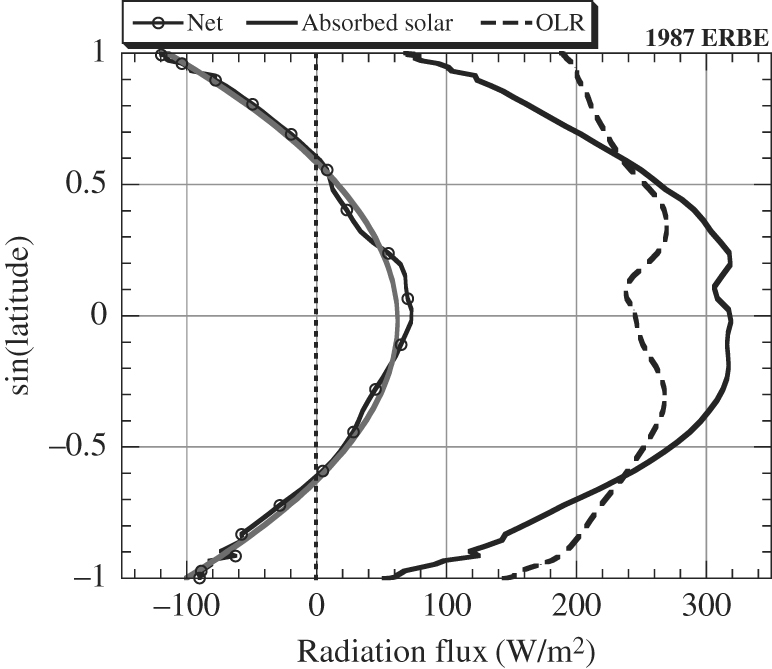
\includegraphics[width=0.5\linewidth]{Figures/GFD/Diff Heating.jpg}
    \caption{Figure from Ray's book showing differential heating. More heat is }
    \label{Diff Heating}
\end{figure}



\section{What is Special About `Geophysical' Fluid Mechanics?}\label{GFD Special}

It is also important to consider what sets \textbf{Geophysical Fluid Dynamics} apart from most other Fluid Dynamics. There are two important properties that \textbf{Geophysical Fluid Dynamics} aim to investigate: \textbf{stratification} and \textbf{rotation}. The effects of these will pop up again and again throughout \hyperref[Geophysical Fluid Dynamics]{GFD}.

\subsection{Stratification}

\textbf{Stratification} is important because the fluids in the atmospheres and oceans are affected by gravity and vary in density. 

You have already seen the effect of stratification when we derived the \hyperref[Hydrostatic Balance]{Hydrostatic Balance}. We found that pressure decreases with height 
\begin{align*}
    \frac{dp}{dz}=-\rho g\\
    \frac{d}{dz}\left( \rho R T \right)=-\rho g\\
    RT \frac{d \rho}{dz} + \frac{}{}
\end{align*}

REFER TO THE BUOYANCY FREQUENCY SECTION IN THE CLOUDS SECTION

[UNDER CONSTRUCTION]

\subsection{Rotation}

\textbf{Rotation} is important because, generally, planets rotate, and the equations of motion ensure that fluid parcels must obey conservation of angular momentum. The idea is as follows: if a fluid parcel is at rest relative to the surface of the Earth, its total angular momentum will actually differ depending on where it is. If it is at the poles, it will have no angular momentum, whereas if it is at the equator, it will have a large amount of angular momentum.

In the previous section, we discussed how differential heating implies that there must be some motion. This motion is required to close the energy budget. Becuase there both is net radiative heating at the equator and net radiative cooling at the poles, and the equator and poles are not heating and cooling over time, there must be some mechanism transfering energy from the equator to the poles. This is achieved by the atmospheres and oceans.

Let us then consider a extremely simple model of this: \textbf{Hadley's Model} of convection as a zonally (zonally means east-west) symmetric equator-to-pole convection cell:
\begin{figure}[H]
    \centering
    \begin{tikzpicture}
        \draw (0,0) -- (5,0) arc[start angle=0, end angle=90, radius=5cm] -- cycle;
        %\draw (5,0) -- (0,0) -- (0,5);
        \draw (0,0) -- (3,0) arc[start angle=0, end angle=90, radius=3cm] -- cycle;
        %\draw (3,0) -- (0,0) -- (0,3);
    \end{tikzpicture}
    \caption{Convection Cell: [FIGURE UNDER CONSTRUCTION]}
\end{figure}

Let us not consider a fluid parcel in this convection cell. We assume that this fluid parcel starts out at the equator at rest (relative to the surface of the Earth) and moves north. We also assume that there are no zonal forces (i.e., no east-west forces) acting on the fluid parcel. This is a highly unrealistic assumption. We further assume that the radius of the Earth $a$ is much larger than the height of the fluid parcel above the Earth.

We know that the total angular momentum of the parcel is approximately equal to the following:
\begin{align*}
    L(\phi,u) = \underbrace{a\cos\phi}_{\vec{r}} \underbrace{\left( \Omega a \cos \phi + u \right)}_{\vec{u}}
\end{align*}
where $a=$ the radius of the Earth, $\phi=$ the latitude, $\Omega=$ the angular velocity of the Earth, and $u=$ the zonal velocity of the fluid parcel relative to the surface of the Earth. The angular momentum is equal to $\vec{r}\times\vec{u}$, the radius $\vec{r}$ times the velocity $\vec{u}$. The radius is equal to $a\cos\phi$ (as it is the radius from the axis of rotation), and the velocity is equal to $\Omega a \cos \phi + u$, the sum of the velocity from the rotation of the Earth and the velocity relative to the Earth.\footnote{
    This is, strictly speaking, incorrect. The angular momentum is a vector (actually a pseudo-vector), so it’s strange to say that the angular momentum is equal to a scalar value. To be more precise, $L(\phi,u)$ is the component of the angular momentum in the direction aligned with the angular velocity of the Earth. In other words parallel the vector pointing directly upwards from the ground at the north pole.
}

Since there are no zonal forces on the air parcel, this implies that the angular momentum is conserved. Setting $L(\phi,u)=const$ imposes the constraint $u=u(\phi)$. We use our assumption that, at $\phi=0$ (the equator), the $u=0$ (fluid parcel is at rest). Therefore, some simple algebra gives us the following relation:
\begin{align*}
    \boxed{u=a\Omega \left( \frac{1}{\cos\phi}-\cos\phi
    \right)}
\end{align*}

Essentially, what this says is that, as the air parcel moves north (as $\phi$ increases), the zonal velocity $u$ also increases! Conservation of angular velocity imposes that the air parcel is deflected as it moves northwards, so fluid parcel motion cannot always be as straightforward on a rotating planet as on a non-rotating planet.

Of course, this model is highly unrealistic. Firstly, it predicts that $u\to\infty$ at $\cos\phi\to\pi/2$, which is clearly unphysical. Secondly, from observations, we pretty much never observe $u\geq\qty{150}{\metre\per\second}$, so the model fails much earlier than $u\to\infty$. In reality, our assumption that there were no zonal forces was a very inaccurate assumption: as horizontal velocities become arbitrarily large, these induce large shears (a shear is when a layer of stuff (e.g., air) is sliding over another layer of stuff (e.g., air)), which in turn induce large forces either from viscous or turbulent eddy stresses.\footnote{For a cursory look at the effect of vertical stresses, refer to this section on \hyperref[Ekman Transport]{Ekman Transport}!}

However, the general moral of the story does apply: there are conservation laws that constrain motion more on rotating planets than non-rotating planets. We find that this will actually be the Material Conservation of Potential Vorticity, but this is jumping ahead a bit.

Looking back, this should be seen as as cursory, highly unrealistic taste of the effect that stratification and rotation might have on dynamics. It won't be much of an exaggeration ot say that we'll spend most of GFD discussing the effects of rotation.

\chapter{The Equations of Motion}\label{EoM GFD}

\section{The Primitive Equations of Motion}

For simplicity we ignore state variables like salinity, humidity, etc., and restrict our attention to a system fully characterised by 6-state variables: the velocity $\vec{u}=(u,v,w)$, pressure $p$, density $\rho$, and temperature $T$. These are governed by six equations: 3 momentum budget equations (\ref{Navier Stokes}), one mass budget equation (\ref{Mass Conservation}), one energy budget equation (\ref{Energy Equation}), and an equation of state (\ref{EoS}). Each term is labelled below:
\begin{gather}
    \boxed{\underbrace{\frac{D\vec{u}}{Dt}}_{\text{Acceleration and Advection}}
    =\overbrace{-\frac{1}{\rho}\vec{\nabla}p}^\text{Pressure Gradients}\underbrace{-g\vec{k}}_\text{Gravity}+\overbrace{\nu\vec{\nabla}^2\vec{u}}^\text{Viscous Dissipation}\underbrace{+\frac{\nu}{3}\vec{\nabla}(\vec{\nabla}\cdot\vec{u})}_\text{}+\overbrace{\vec{F}}^\text{Other Forces}}
    \label{Navier Stokes}
    \\
    \boxed{\underbrace{\frac{D\rho}{Dt}}_\text{Change in Mass of Fluid Parcel}
    +
    \overbrace{\rho\vec{\nabla}\cdot\vec{u}}^\text{Convergence/Divergence of Mass}=0}
    \label{Mass Conservation}
    \\
    \boxed{\underbrace{c_p\frac{DT}{Dt}}_\text{Energy of Air Parcel}-\overbrace{\frac{\beta T}{\rho}\frac{Dp}{Dt}}^\text{Heating by Compression}=\underbrace{Q}_\text{Diabatic Heating (e.g., by radiation)}}
    \label{Energy Equation}
    \\
    \boxed{\rho=\underbrace{\rho(T,p,\ldots)}_{\text{Equation of State}}}
    \label{EoS}
\end{gather}

\noindent where $\frac{D}{Dt}=\frac{\partial}{\partial t}+\vec{u}\cdot\vec{\nabla}$ is the material derivative; $g=$ gravitational acceleration; $\vec{k}=$ unit vector towards the centre of the Earth; $\nu=$ kinematic viscocity; $\vec{F}=$ other forces per unit mass (e.g., friction); $c_p=$ heat capacity per unit mass; $\beta=-\frac{1}{\rho}\frac{\partial \rho}{\partial T}$ thermal expansion coefficient; and $Q=$ heating per unit mass.

However, the equations currently are not fit for purpose. First, these equations are written for a coordinate system that is \textit{inertial} (non-accelerating) and \textit{cartesian}. However, the surface of the Earth is curved and the Earth is rotating\footnote{or so NASA and the lizard overlords would have you think!}, and we wish to describe what is going on \textit{here} with us. Furthermore, it would be quite demanding (computationally and conceptually) to adopt an inertial non-curved coordinate system, as then you'd have to, for example, keep track of the fact that the mountains keep moving. 

Second, these equations are currently too complicated to be analytically tractable. We will make various approximations later to simplify the equations of motion, however we should note that many of the terms we neglect cannot be neglected in a weather forecast or climate model.

\section{Simplifications}

\subsection{Rotating Coordinate Systems}

As already mentioned, the momentum budget equation applies for an \textit{inertial coordinate system}, i.e., a coordinate system which is not accelerating. However we wish to describe the dynamics in a rotating coordinate system which rotates with the Earth (or planet). Our goal now is to  find a relation between the time derivative of some arbitrary vector $\vec{A}$ in an inertial coordinate system $\left(\frac{d\vec{A}}{dt}\right)_I$ and the time derivative in a rotating coordinate system $\left(\frac{d\vec{A}}{dt}\right)$.

We consider two coordinate systems: an \textit{inertial} coordinate system and a \textit{rotating} coordinate system. Both systems share an origin, but the \textit{inertial} coordinate system rotates with a constant angular velocity $\vec{\Omega}$ where $|\vec{\Omega}|$ is the angular speed (in \qty{}{\radian\per\second}) and $\vec{\Omega}$ points along the axis of rotation.

Now consider some arbitrary vector $\vec{A}(t)$ in or rotating coordinate system. The time derivative in the inertial coordinate system $\left(\frac{d\vec{A}}{dt}\right)_I$ is related to the time derivative in the rotating coordinate system $\left(\frac{d\vec{A}}{dt}\right)_R$ as follows (see Figure \ref{Inertial to Rotating}):
\begin{figure}[H]
    \centering
    \begin{subfigure}{0.45\linewidth}
        \centering
        \begin{tikzpicture}
            \draw[->] (0,0) -- (3.5,0) node[anchor=west] {$x_R$};
            \draw[->] (0,0) -- (0,3.5) node[anchor=south] {$y_R$};
            \draw[thick,->] (0,0) -- (3,2) node[anchor= north] {$\vec{A}(t)$};
            \draw[thick,->] (0,0) -- (2,3) node[anchor=south] {$\vec{A}(t+\delta t)$};
            \draw[ultra thick,->] (3,2) -- (2,3) {};
            \node[] at (3.5,2.75) {$\delta t \left( \frac{\partial \vec{A}}{\partial t} \right)_R$};
        \end{tikzpicture}
        \caption{Change in $\vec{A}$ in the Rotating Coordinate System}
        \label{Rotating}
    \end{subfigure}
    \hfill
    \begin{subfigure}{0.45\linewidth}
        \centering
        \begin{tikzpicture}
            \draw[->] (0,0) -- (3.5,0) node[anchor=west] {$x_I$};
            \draw[->] (0,0) -- (0,3.5) node[anchor=east] {$y_I$};
            \draw[thick,->] (0,0) -- (3,2) node[anchor=west] {$\vec{A}(t)$};
            %\draw[dotted,->] (0,0) -- (2,3) node[anchor=south] {};
            \draw[thick,->] (0,0) -- (0.853,3.503) node[anchor=south east] {$\vec{A}(t+\delta t)$};
            \draw[ultra thick,->,dashed] (3,2) -- (2,3) {};
            \node[] at (3.5,2.75) {$\delta t \, \left( \frac{\partial \vec{A}}{\partial t} \right)_R$};
            \draw[ultra thick,->,dashed] (2,3) -- (0.853,3.503) {};
            \node[] at (2,3.75) {$\delta t \vec{\Omega}\times\vec{A}$};
            \draw[->,dashed] (0,0) -- (3.289,1.197) node[anchor=west] {$x_R$};
            \draw[->,dashed] (0,0) -- (-1.197,3.289) node[anchor=east] {$y_R$};
            \draw[ultra thick,->] (3,2) -- (0.853,3.503);
            \node[] at (1.5,2) {$\delta t \left( \frac{\partial \vec{A}}{\partial t} \right)_I$};
        \end{tikzpicture}
        \caption{Change in $\vec{A}$ in the Inertial Coordinate System}
        \label{Inertial}
    \end{subfigure}
    \caption{The change in $\vec{A}$ in a rotating (\ref{Rotating}) and inertial (\ref{Inertial}) coordinate system. As seen in \ref{Inertial}, the change in the inertial coordinate system $\delta t \left( \frac{\partial \vec{A}}{\partial t} \right)_I$ (thick arrow) is equal to sum of the change in the rotating coordinate system $\left( \delta t \left( \frac{\partial \vec{A}}{\partial t} \right)_R \right)$ \textit{and} the rotation of the rotating coordinate system $\left(\delta t\,\vec{\Omega}\times\vec{A} \right)$ (thick dashed arrows).}
    \label{Inertial to Rotating}
\end{figure}
\begin{align}
    \left(\frac{d\vec{A}}{dt}\right)_I=\left(\frac{d\vec{A}}{dt}\right)_R+\vec{\Omega}\times\vec{A}
    \label{Rotating Relation}
\end{align}

If we let $\vec{A}=\vec{r}$, where $\vec{r}$ is the position of our fluid parcel, we can apply Equation \ref{Rotating Relation} twice to obtain an expression for the acceleration of a fluid parcel in a rotating coordinate system.
\begin{align*}
    \vec{u}_I &= \left( \frac{d\vec{r}}{dt} \right)_I\\
    &= \left( \frac{d\vec{r}}{dt} \right)_R+\vec{\Omega}\times \vec{r}\\
    \vec{u}_I & = \vec{u}_R+\vec{\Omega}\times \vec{r}\\
    \therefore \vec{a}_I & =
    \left( \frac{d\vec{u}_I}{dt} \right)_I\\
    &= \left( \frac{d\vec{u}_I}{dt} \right)_R+\vec{\Omega}\times \vec{u}_I\\
    &= \left( \frac{d\vec{u}_R}{dt} \right)_R
    +\vec{\Omega}\times\left( \frac{d\vec{r}}{dt} \right)_R
    +\vec{\Omega}\times\left( 
        \vec{u}_R+\vec{\Omega}\times \vec{r}
     \right)\\
    &=\vec{a}_R+2\vec{\Omega}\times\vec{u}_R+\vec{\Omega}\times\vec{\Omega}\times\vec{r}
\end{align*}

Therefore the acceleration in the rotating frame of reference $\vec{a}$ is equal to the acceleration in a inertial coordinate system summed with two fictitious\href{https://xkcd.com/123/}{$^*$}  forces: the \textbf{centrifugal force} and the \textbf{coriolis force}.
\begin{align}
    \vec{a}_R=\vec{a}_I+\underbrace{2\vec{\Omega}\times\vec{u}_R}_\text{Coriolis}
    +\underbrace{\vec{\Omega}\times\vec{\Omega}\times\vec{r}}_\text{Centrifugal}
\end{align}

The \textbf{centrifugal force} is the force that pushes objects away from the axis of rotation. This is the force that makes your arms fling out if you spin. The \textbf{coriolis force} is the force that diverts moving objects which move away or towards the axis of rotation. 

We have thus transformed Equation \ref{Navier Stokes} into a rotating coordinate system:
\begin{align}
    \frac{D\vec{u}}{Dt}+2\vec{\Omega}\times\vec{u}+\frac{1}{\rho}\vec{\nabla}p+g\vec{k}=-\vec{\Omega}\times\vec{\Omega}\times\vec{r}+\nu\vec{\nabla}^2\vec{u}+\frac{\nu}{3}\vec{\nabla}(\vec{\nabla}\cdot\vec{u})+\vec{F}\label{Navier Stokes Rotating}
\end{align}

\subsection{Local Cartesian Coordinates}

We have just learnt how to deal with coordinate systems that vary with time. We will now skim over (since the details aren't that interesting) how to deal with coordinate systems that vary with space.

We wish to use a coordinate system that follows the surface of the Earth, with the basis vectors $\hat{x}$, $\hat{y}$, $\hat{z}$, pointing in the east, north, and upwards (away from the centre of the Earth) directions. In this coordinate system, we define the position and velocity coordiates $(x,y,z)$ and $(u,v,w)$ as indicating distance and velocity in the east, north, and upwards directions, respectively. We further define the latitude $\phi\in[-\frac{\pi}{2},\frac{\pi}{2}]$ ($\phi=0$ indicates the equator, $\phi=\pm\frac{\pi}{2}$ is the north/south pole) and the radial distance $r$ where $r=a+z$ where $a=$ the radius of the Earth (see Figure \ref{LocCartes}).
\begin{figure}[H]
    \centering
    \scalebox{1.4}{
    \begin{tikzpicture},
        \begin{scope}[3d view={125}{25.26}]
            \draw[->,opacity=0.7] (0,0,0) -- (1.5,0,0) node[anchor=north east] {$x'$};
            \draw[->,opacity=0.7] (0,0,0) -- (0,1.5,0) node[anchor=north] {$y'$};
            \draw[->,opacity=0.7] (0,0,0) -- (0,0,1.5) node[anchor=north west] {$z'$};
            \draw[-,dashed] plot[domain=0:400,samples=41,smooth]({1.5*sin(\x)},{1.5*cos(\x)},{0});
            \draw[-,dashed] plot[domain=0:400,samples=41,smooth]({1.5*cos(0)*sin(\x)},{1.5*sin(0)*sin(\x)},{1.5*cos(\x)});
            \draw[-,dashed] plot[domain=0:360,samples=41,smooth]({1.0607*sin(\x)},{1.0607*cos(\x)},{1.0607});
            \coordinate (A) at (1.0607,0,1.0607);
            \draw[-] (0,0,0) -- (A);
            \draw[->,thick,mymagenta] (A) -- (0.7071,0,1.414);
            \draw[->,thick,mymagenta] (A) -- (1.0607,0.5,1.0607);
            \draw[->,thick,mymagenta] (A) -- (1.414,0,1.414);
            %\filldraw[fill=myorange,opacity=0.5] (1,0,0) .. controls +(0,0,0.8) and +(0.5,0.2,0) .. (0.7071,0,0.7071) -- (0,0,0);
            \filldraw[fill=myorange,opacity=0.5] (1,0,0) .. controls +(0,0,0.5) and +(0.1,0,-0.1) .. (0.7071,0,0.7071) -- (0,0,0);
        \end{scope}
        \begin{scope}
            \draw[-,dashed] plot[domain=0:400,samples=41,smooth]({1.5*sin(\x)},{1.5*cos(\x)});
            \node at (-0.5,1.2) {$y$};
            \node at (-0.2,0.8) {$x$};
            \node at (-0.8,0.95) {$z$};
            \node at (-0.35,0.04) {$\phi$};
        \end{scope}
    \end{tikzpicture}}
    \caption{Local Carteisan Coordinates. $(x',y',z')$ indicate our global cartesian coordinate system, while $(x,y,z)$ indicate our local cartesian coordinate system in magenta arrows.}
    \label{LocCartes}
\end{figure}
Churning through the algebra, we get:
\begin{align*}
    \frac{Du}{Dt}-\left( 2\Omega+\frac{u}{r\cos\phi} \right)\left( v\sin\phi-w\cos\phi \right)+\frac{1}{\rho}\frac{\partial p}{\partial x}
    =F_x\\
    \frac{Dv}{Dt}+\frac{wv}{r}+\left( 2\Omega+\frac{u}{r\cos\phi} \right)u\sin\phi+\frac{1}{\rho}\frac{\partial p}{\partial y}=F_y\\
    \frac{Dw}{Dt}-\frac{u^2+v^2}{r}-2\Omega u \cos\phi+\frac{1}{\rho}\frac{\partial p}{\partial z}+g=F_z
\end{align*}
where we have lumped together all the terms on the right-hand-side of \ref{Navier Stokes Rotating} into the $F_x, F_y, F_z$. Many of the extra terms $\left( \text{e.g., the } \frac{wv}{r} \text{ term}\right)$, are due to the fact that we have adopted a local cartesian system, in which the coordinate system changes as we move over the Earth. 

\subsection{Incompressibility}

Our final assumption is regarding the compressibility of fluids. If a fluid has constant density ($\rho=\rho_0=const$), then by Equation \ref{Mass Conservation} $\vec{\nabla}\cdot\vec{u}=0$ applies. We say that this fluid is \textbf{incompressible}: every bit of fluid that enters some volume must also leave.

We will end up assuming that $\vec{\nabla}\cdot\vec{u}=0$. Note that this should seem, to you, a \textbf{highly} dubious assumption. First, we know that sound waves are possible (after all we can hear, both on land and in water), but sound waves are impossible in an incompressible fluid. Second, and more importantly, we know that the atmosphere is approximately an ideal gas, which can have its density changed if warmed or cooled. For the ocean, we know that temperature, salinity, and pressure all change the density of seawater.

However, we are justified to use this equation if we assume that density variations $\delta p = \delta p (x,y,z,t)$ are much smaller than the background density $\rho_0$.
\begin{align}
    \therefore \boxed{\vec{\nabla}\cdot \vec{u}=0}\label{Incompressible}
\end{align}

However, I should emphasise that this does \textit{not} allow us to assume that $\frac{D\rho}{Dt} = \frac{D\delta \rho}{Dt} = 0$ applies.

\subsection{Scale Analysis}\label{Scale Analysis}

Finally, we make a few phenomenological simplifications. We do this here for simplicity, but our results are not general or particularily robust: these terms are essential in climate/weather models. We do this here by performing a \textbf{scale analysis}: we estimate the size of quantities by their typical values (found empirically), then ignore terms that are much smaller than the other terms. We never neglect the pressure gradient term. \vspace{5mm}

\noindent
\begin{tabular}{|p{5.8cm}|p{1.4cm}|p{4cm}|p{4cm}|}
\hline
    Scale & Symbol & Terms Approximated & Typical Magnitude \\
\hline
\hline
Horizontal Scale & $L$ & $\frac{\partial}{\partial x}\sim\frac{1}{L}$, $\frac{\partial}{\partial y}\sim\frac{1}{L}$& \qty{e6}{\metre}\\
\hline
Vertical Scale & $H$ & $\frac{\partial}{\partial z}\sim\frac{1}{H}$& \qty{e4}{\metre}\\
\hline
Horizontal Velocity & $U$ & $u\sim U$, $v\sim U$& \qty{10}{\metre\per\second}\\
\hline
Vertical Velocity & $W$ & $w\sim W$& \qty{e-2}{\metre\per\second}\\
\hline
Time Scale & $T$ & $\frac{\partial}{\partial t}\sim\frac{1}{T}$& \qty{e5}{\second}\\
\hline
Density & $\rho$ & $\rho\sim\rho$& \qty{1}{\kilogram\per\second}\\
\hline
Earth's Radius & $a$ & $r\sim a$& \qty{6.4e6}{\metre}\\
\hline
Rotation Rate & $\Omega$ & $\Omega\sim\Omega$ & \qty{e-4}{\per\second}\\
\hline
Acceleration of Gravity & $g$ & $g\sim g$ & \qty{10}{\metre\per\second\squared}\\
\hline
\end{tabular}\newline

I do not write out all the details here, as they would easily take multiple pages. If you are curious about the details, refer to the mini-scale analysis I do in deriving \ref{Hydrostatic GFD}. A more rigorous method would be non-dimensionalisation, but this is overkill for our purposes. Again, if you are curious about the details, refer to the mini-non-dimensionalisation I do in deriving the \hyperref[Rossby Number]{Rossby Number}. 

Suffice it to say that we eliminate many terms through this scale analysis. This includes any terms that feature the viscosity $\nu$, the centrifugal force, and many terms arising from our local cartesian coordinate system. 

After eliminating small terms, we get our final simplified set of equations. 

\section{The Simplified Equations of Motion}

\begin{fact}{The Simplified Equations of Motion for GFD}{Eqns for GFD Box}\label{Eqns for GFD Box}
    We define the horizontal gradient operator taken at constant $z$ as $\vec{\nabla}_h=\left( \frac{\partial}{\partial x},\frac{\partial}{\partial x},0 \right)^T$, the horizontal velocity as $\vec{u}_h=\left( u,v,0 \right)^T$, the horizontal forces as $\vec{F}_h$, and the \textbf{coriolis parameter} as $f=2\Omega\sin\phi$ where $\phi=$ the latitude.

    The simplified equations of motion we will be using are as follows: \vspace{2mm}

    \begin{minipage}{0.48\linewidth}
        \centering
        \textbf{Vertical Momentum Balance:}
        \begin{gather}
            \label{Vertical Approximate}
            \BOX{\frac{Dw}{Dt}+\frac{1}{\rho}\frac{\partial p }{\partial z}+g=F_z}
        \end{gather}
    \end{minipage}
    \hfill
    \begin{minipage}{0.48\linewidth}
        \centering
        \textbf{Incompressibility:}
        \begin{gather}
            \label{Incompressibility}
        \BOX{\vec{\nabla}\cdot\vec{u}=0}
        \end{gather}
    \end{minipage}

    \vspace{2mm}
    \centering
    \textbf{Horizontal Momentum Balance:}
    \begin{gather}
        \label{Horizontal Approximate}
        \BOX{\underbrace{\frac{D\vec{u}_h}{Dt}}_\text{acceleration and advection}+
        \overbrace{f\vec{k}\times\vec{u}_h}^\text{coriolis}+
        \underbrace{\frac{1}{\rho}\vec{\nabla}_hp}_\text{horizontal pressure gradients}=\overbrace{\vec{F}_h}^\text{other forces}}
    \end{gather}
\end{fact}

Physically, the \textbf{coriolis parameter} $f=2\Omega \sin \phi$ is the planetary vorticity: it is the vorticity that a fluid parcel at rest (relative to the surface of the Earth) has in the $z$-direction. Note that we've ignored the Energy Equation (\ref{Energy Equation}). This equation is important, but we don't really discuss it in C5.

We will mostly be dealing with the horizontal momentum equation \ref{Horizontal Approximate}, so it is worth detailing the meanings of each terms. The first term, $\frac{D\vec{u}_h}{Dt}$ is the material derivative of $\vec{u}_h$. It represents the acceleration of $\vec{u}_h$ and the advection of $\vec{u}_h$. The $f\vec{k}\times\vec{u}_h$ term is the acceleration due to coriolis. The $\frac{1}{\rho}\vec{\nabla}_h p$ is the force due to the horizontal pressure gradient. Finally, the $\vec{F}_h$ term is external forces, e.g., friction, wind-forcing, etc.

\chapter{The Fundamental Diagnostic Relations}\label{Dia Relations}

\section{Hydrostatic Balance (Approximate Vertical Momentum Balance)}\label{App Vert Bal}

We now make further approximations to extract physical intuition. Consider \ref{Vertical Approximate}, and again perform a scale analysis and assume that $F_z\approx 0$.
\begin{align*}
    &&\frac{Dw}{Dt} &+
    & \frac{1}{\rho}\frac{\partial p}{\partial z}+
    &g=0
    \\
    &\underbrace{\frac{\partial w}{\partial t}}_{\frac{W}{T}}+ 
    &\underbrace{u\frac{\partial w}{\partial x} 
    + v\frac{\partial w}{\partial y}}_{U\frac{W}{L}}+ 
    &\underbrace{w\frac{\partial w}{\partial z}}_{W\frac{W}{H}}+ 
    &\frac{1}{\rho}\frac{\partial p}{\partial z}+
    &g=0
    \\
    &\sim\frac{W}{T}+
    &\sim U\frac{W}{L}+
    &\sim\frac{W^2}{H}+ 
    &\frac{1}{\rho}\frac{\partial p}{\partial z}+
    &g=0
    \\
    \therefore
    &\frac{\text{\qty{e-2}{\metre\per\second}}}{\text{\qty{e5}{\second}}}+ 
    &\text{\qty{10}{\metre\per\second}}\frac{\text{\qty{e-2}{\metre\per\second}}}{\text{\qty{e6}{\metre}}}+ 
    &\frac{\left( \text{\qty{e-2}{\metre\per\second}} \right)^2}{\text{\qty{e4}{\metre}}}+ 
    &\frac{1}{\rho}\frac{\partial p}{\partial z}+
    &\text{\qty{10}{\metre\per\second\squared}}=0
    \\
    &\text{\qty{e-7}{\metre\per\second\squared}}+
    &\text{\qty{e-7}{\metre\per\second\squared}}+
    &\text{\qty{e-8}{\metre\per\second\squared}}+
    &\frac{1}{\rho}\frac{\partial p}{\partial z}+
    &\text{\qty{10}{\metre\per\second\squared}}=0
    \\
    &\bcancel{\text{\qty{e-7}{\metre\per\second\squared}}}+
    &\bcancel{\text{\qty{e-7}{\metre\per\second\squared}}}+
    &\bcancel{\text{\qty{e-8}{\metre\per\second\squared}}}+
    &\frac{1}{\rho}\frac{\partial p}{\partial z}+
    &\text{\qty{10}{\metre\per\second\squared}}=0
\end{align*}

As seen then, many of the acceleration terms (the terms in the $\frac{Dw}{Dt}$) are 8 orders of magnitutde smaller than gravity! As such, the only term that can balance the gravity term is the pressure gradient. We thus neglect all other terms and derive again:

\begin{fact}{Hydrostatic Balance}{Hydrostatic GFD Box}\label{Hydrostatic GFD Box}
Hydrostatic Balance governs the vertical pressure variation in a fluid if we assume that vertical acceleration (and advection) is small.
    \begin{equation}\label{Hydrostatic GFD}
    \BOX{
        \frac{\partial p}{\partial z}=-\rho g
    }
    \end{equation}
Pressure decreases with height in order to balance the force of gravity.
\end{fact}

Physically, hydrostatic balance is a force/momentum balance in the vertical direction, where the force of gravity is balanced by the vertical pressure gradient. Notice now the difference between the Hydrostatic Balance I have written here (\ref{Hydrostatic GFD}) and the Hydrostatic Balance I have written in the \hyperref[Thermodynamics]{Thermodynamics} Section (\ref{Hydrostatic Balance}): I have written it here with a partial derivative. Strictly, it should have been a partial derivative before too, but I write it here to note that we are now considering horizontal variations as well as vertical variations.

For an ideal gas, one can substitute for $\rho$ using \ref{Ideal Gas}:
\begin{align}\label{Hydrostatic Ideal Gas}
    \boxed{\frac{\partial \ln p}{\partial z}=-\frac{g}{RT}}
\end{align}

\section{Geostrophic Balance (Approximate Horizontal Momentum Balance)}\label{App Horiz Bal}

\subsection{Rossby Number and Non-Dimensionalisation}

Let us now consider the horizontal momentum equation \ref{Horizontal Approximate} and let $\vec{F}_h\approx 0$ for now. We nondimensionalise the equations by defining dimensionless hatted variables and choosing characteristic scales such that the dimensionless hatted variables are of order 1:
\begin{align*}
    t=[t]\hat{t}\text{   ;   }
    \vec{r}=L\vec{\hat{r}}\text{   ;   }
    \vec{u}_h=[u_h]\vec{\hat{u}}_h\text{   ;   }
    p=[p]\hat{p}
\end{align*}

So, for example, $[t]= $ the timescale with dimensions of time and $L= $ the lengthscale with dimesions of length, while $\hat{t}$ and $\vec{hat{r}}$is the dimensionless time/position variables. We \textit{must} pick these scales $[t]$, $L$, $[u_h]$, $[p]$ \textit{such that} the hatted variables ($\hat{t}$,$\vec{\hat{r}}$, $\vec{\hat{u}}_h$, $\hat{p}$) are of order one, so we're constrained by the system under consideration.\footnote{
    In fact we've already made an implicit assumption that the system is roughly isotropic, which means that we can choose $[v]=[u]=[u_h]$ and $[x]=[y]=L$.  
} We now substitute these variables into \ref{Horizontal Approximate}:
\begin{align*}
    \frac{[u_h]}{[t]}\frac{\partial\vec{\hat{u}}_h}{\partial t}+\frac{[u_h]^2}{L}\left( \vec{\hat{u}}_h\cdot\vec{\hat{\nabla}} \right)\vec{\hat{u}}_h+[u_h]f\vec{k}\times\vec{\hat{u}}_h+[p]\frac{1}{\rho}\vec{\nabla}_h\hat{p}=0
\end{align*}
where $\vec{\hat{\nabla}}=(\partial/\partial \hat{x},\partial/\partial \hat{y})^T$ is the non-dimesional nabla operator. Dividing by $f[u_h]$, we get:
\begin{align*}
    \underbrace{\boxed{\frac{1}{f[t]}}}_{\equiv St}\frac{\partial\vec{\hat{u}}_h}{\partial t}+\underbrace{\boxed{\frac{[u_h]}{fL}}}_{\equiv Ro}\left( \vec{\hat{u}}_h\cdot\vec{\hat{\nabla}} \right)\vec{\hat{u}}_h+\vec{k}\times\vec{\hat{u}}_h+\underbrace{\boxed{\frac{[p]}{\rho f [u_h]}}}_{\equiv P}\vec{\nabla}_h\hat{p}=0
\end{align*}

We thus see three non-dimesional coefficients appear in front of each of the terms in each equation: $St$, $Ro$, and $P$.\footnote{
    While $St$ and $Ro$ are standard nomenclature for these non-dimesional quantities, $P$ is not.
} These non-dimesional coefficients compare the relative size and therefore importance each term in the Horizontal Momentum equation. You might expect there to be four non-dimesional coefficients because there were four scales we could choose, but there are only three because this fourth non-dimensional coefficient is set by the Horizontal Momentum equation itself: all the terms on the left hand side \textit{must} sum to $0$.

Now, written just in terms of the non-dimensional coefficients, we write the (isotropic) non-dimensional horizontal momentum equation:
\begin{align}
    \label{Horizontal Approximate nondim}
    \underbrace{St\,\frac{\partial\vec{\hat{u}}_h}{\partial t}}_{O(St)}+
    \underbrace{Ro\,\left( \vec{\hat{u}}_h\cdot\vec{\hat{\nabla}} \right)\vec{\hat{u}}_h}_{O(Ro)}+
    \underbrace{\vec{k}\times\vec{\hat{u}}_h}_{O(1)}+
    \underbrace{P\,\vec{\nabla}_h\hat{p}}_{O(P)}=0
\end{align}

Note that because we have nondimensionalised such that each variable is of order one, the $\vec{k}\times\vec{\hat{u}}_h$ is always of order one, while the other terms are of order $St$, $Ro$, and $P$, respectively.

The physical interpretation of each coefficient is as follows: $St$ represents the ratio of the intrinsic timescale of the system $[t]$ (set by dynamics of the particular problem under consideration) and the timescale of the rotation of the planet $1/f$. This intrinsic timescale could be set, for example, by the stratification (for example the Brunt Vasalla frequency you encountered in Clouds PUT REFERENCE HERE $[t]=1/N$). Other times, if there is no intrinsic timescale, the timescale is often set by the advection $[t]=L/[u_h]$. If this timescale is much shorter than the rotation timescale (i.e., if $[t]\ll 1/f$) then $St\gg 1$, so the left-hand most term is much larger than the rotation $\vec{k}\times\vec{\hat{u}}_h$ term. Physically, this means that the local rate of change `doesn't see' the fact that the planet is rotating. This is because everything happens so quickly that the planet hasn't rotated much to affect events. This is what happens on human scales: if I throw a ball at you then this takes much less time than $1/f\sim$ 1 day, so we don't notice the Earth rotating.

For simplicity, we simply assume at this point that the following obtains: that the timescale is set by advection or something slower than advection such that $[t]\geq L/[u_h]$ (i.e., we are never interested in stuff happening on very time-scales shorter than the advective timescale). As such, we can approximate $St\leq Ro$ so that we get:
\begin{align*}
    Ro\,\left( \frac{\partial\vec{\hat{u}}_h}{\partial t}+\left( \vec{\hat{u}}_h\cdot\vec{\hat{\nabla}} \right)\vec{\hat{u}}_h\right)+\vec{k}\times\vec{\hat{u}}_h +P\,\vec{\nabla}_h\hat{p}=0
\end{align*}

We can now explain the \textbf{Rossby Number} $Ro$ very easily. $Ro$ compares the effect of advection/acceleration to rotation: if $Ro \ll 1$ (the \textbf{Rossby Number} is small), then rotation is important and dominates dynamics. If $Ro \gg 1$ (the \textbf{Rossby Number} is large), then the flow evolves in such a way where coriolis is negligible.

\begin{fact}{Rossby Number}{Rossby box}\label{Rossby Box}
    We define the dimensionless \textbf{Rossby Number} $Ro$, which encodes the relative importance of (planetary) rotation and advection/acceleration terms, as follows:
    \begin{gather}
        \label{Rossby Number}
        \BOX{
            Ro=\frac{U}{fL}
        }
    \end{gather}
    where $U=$ the horizontal velocity scale, $f=$ the coriolis parameter, and $L=$ the horizontal length scale.
    
    If $Ro\ll 1$, then the rotation of the planet is important, and the flow should be approximately \textbf{Geostrophic}. If $Ro\gg 1$, then acceleration/advection is important.
\end{fact}

Note that I have not specified $P$. This is because we expect the pressure scale $P$ to be set by the dynamics governed by the \hyperref[Horizontal Approximate]{Horizontal Momentum Equation}. If $Ro\ll 1$, then we expect $P$ to be of order $1$ in order to balance the coriolis $\vec{k}\times\vec{\hat{u}}_h$ term. If $Ro\gg 1$, then we expect $P$ to be of order $Ro$ in order to balance the advection/acceleration $D\vec{\hat{u}}_h/Dt$ term. 

We can also write the Rossby Number in terms of a ratio between the planetary vorticity and relative vorticity. The planetary vorticity $\omega_{planetary}$ is the angular velocity of a fluid parcel due to the rotation of the Earth, and scales as $f$. The relative vorticity is the vorticity of our fluid parcel in our coordinate system which is rotating with the Earth, and scales as $\omega_{relative}\sim[\vec{\omega}]_z=[\vec{\nabla}\times\vec{u}_h]_z\sim U/L$. Therefore:
\begin{align}
    Ro &= \frac{\omega_{relative}}{\omega_{planetary}}\\
    &\sim\frac{U/L}{f}
\end{align}

The actual size of $Ro$ depends on the kind of system we are considering: i.e., what are the length-scales and velocity-scales of the system. But it also, crucially, depends on the coriolis parameter $f=2\Omega\sin\phi$. $f=0$ at or near the equator, and so it is unlikely that $Ro$ will ever be small near the equator. However, this does not imply that rotation is unimportant near the equator, but it does imply that the flow is probably not geostrophic near the equator.

Much of the theory of GFD that we will discuss will require the system to be geostrophic, or approximately geostrophic, which means that much of what we apply will only be very accurate in the mid-/high-latitudes (coincidentally where we are!). It is worth bearing this in mind.

\subsection{Geostrophic Balance}

If $Ro\ll 1$ and all other forces are negligible, then rotation dominates dynamics. We can therefore neglect external forces (set $\vec{F}_h\approx0$) and acceleration and advection (set $D\vec{u}_h/Dt\approx0$) in Equation \ref{Horizontal Approximate nondim} (the horizontal momentum equation). Because the equation must equal $0$, we are forced to conclude that $P$ is of order one, so Equation \ref{Horizontal Approximate nondim} and therefore Equation \ref{Horizontal Approximate} must be a balance between the horizontal pressure gradient force and the coriolis force.\footnote{
    You might be suspicious from what I've said. After all, $Ro$ depends on velocity-scale $U$ and length-scale $L$, which we expect should be set by the dynamics and governed by the underlying equations of motion!

    In other words, \textit{if} $Ro\ll 1$, then we expect the system to be in geostrophic balance, but why is $Ro\ll 1$ in the first place, and why would our atmosphere/ocean system tend towards a state such that $Ro\ll 1$ holds?

    The answer lies in the phenomenon of \textbf{geostrophic adjustment}, which you can read about in Vallis' textbook on GFD \cite{Vallis}. The gist is this: anomalies and instabilities on a rotating planet cannot simply propagate away (e.g., via gravity flattening the surface of a fluid, for example) from the source to make the fluid more homogenous. It cannot because the fluid is on a rotating planet, and so must preserve some form of angular momentum.

    As such, after anomalies begin propagating away, there will come a point (where it reaches the anomaly reaches the \hyperref[SW Def Radius Box]{Rossby Deformation Scale}) where it is deflected by the coriolis force, and the system evolves \textit{towards} geostrophic balance.

    More details, again, can be found in Vallis' book.
} 

\begin{fact}{Geostrophic Balance}{Geostrophic Box}\label{Geostrophic Box}
    A flow is geostrophic if the dominant terms in the horizontal momentum balance equation (Equation \ref{Horizontal Approximate}) are the coriolis force and the pressure gradient force. As such, these terms must balance as follows:
    \begin{align}
        \label{Geo Bal}
        \BOX{f\vec{k}\times\vec{u}_h=-\frac{1}{\rho}\vec{\nabla}_hp}
    \end{align}
    This results in a velocity field determined by the pressure gradient as follows (Exercise: Show that Equation \ref{Geostrophic Balance} satisfies Equation \ref{Geo Bal} for any arbitrary pressure field $p$):
    \begin{align}\label{Geostrophic Balance}
        \boxed{\vec{u}_h=\frac{1}{\rho f}\vec{k}\times\vec{\nabla}_hp}
    \end{align}
\end{fact}

Written out, each component of $\vec{u}_h=(u,v)^T$ is as follows:

\begin{minipage}{0.45\linewidth}
    \begin{align*}
        \BOX{u = -\frac{1}{\rho f}\frac{\partial p}{\partial y}}
    \end{align*}
\end{minipage}
\hfill
\begin{minipage}{0.45\linewidth}
    \begin{align*}
        \BOX{v = \frac{1}{\rho f}\frac{\partial p}{\partial x}}
    \end{align*}
\end{minipage}

\vspace{2 mm} Recall that the horizontal gradient of pressure $\vec{\nabla}_h p$ points in the direction of increasing $p$. Equation \ref{Geo Bal} shows that the coriolis force, which pushes a fluid at right angles to its velocity, balances the pressure gradient force, which pushes a fluid from areas of high pressure to areas of low pressure.

We can use Equation \ref{Ideal Gas} to show that, for an ideal gas, geostrophic balance may be written as follows:
\begin{align}
    \label{Geostrophic Ideal Gas}
    \vec{u}_h=\frac{RT}{ f}\vec{k}\times\vec{\nabla}_h\ln p
\end{align}

\subsection{Cyclones and Anti-Cyclones}\label{Cyclones}

The horizontal velocity field is thus set by the horizontal pressure field in Equation \ref{Geostrophic Balance}. 

Recall from our \hyperref[VC Interp]{Vector Calculus Interpretation Box} that the contours of constant $p$ are always perpendicular to the gradient $\vec{\nabla}_h p$ of the pressure field $p$, and point from areas of low pressure to areas of high pressure. Recall further that a cross product of two vectors $\vec{a}\times\vec{b}$ is always perpendicular to both $\vec{a}$ and $\vec{b}$.\footnote{
    The way I like to remember how this works is the right-hand rule. Make a cartesian coordinate system with your right hand: first make a thumbs up with your right hand, then point your index finger away from you, then point your middle fingle to your left.

    Now consider $\vec{a}\times\vec{b}=\vec{c}$. If you align $\vec{a}$ with your thumb, then align $\vec{b}$ with your index finger, then $\vec{c}$ will be pointing in the direction of your middle finger!

    Further note: (I think?) this is why we call certain cartesian coordinate systems a right handed coordinate system, because $\hat{x}\times\hat{y}=\hat{z}$, where $\hat{x}$, $\hat{y}$, $\hat{z}$ are the unit vectors pointing in the $x$, $y$, and $z$ directions.
}

Therefore, if the flow is geostrophic, then $\vec{u}_h$ flows parallel \textbf{isobars} (an isobar is defined as a contour of constant $p$). It is not difficult to verify this by showing that $\vec{u}_h\cdot\vec{\nabla}_h p=0$.

If you consider blobs of higher or lower pressure (which I will draw with circles for simplicity), you will see that the horizontal velocity flows either clockwise or anticlockwise around the areas of high or low pressure. Whether it is clockwise or anticlockwise will depend if we are in the northern hemisphere (so that $f=2\Omega\sin\phi>0$ obtains) or in the southern hemisphere (so that $f=2\Omega\sin\phi<0$ obtains).

\begin{figure}[H]
    \centering
    \begin{subfigure}{0.45\linewidth}
        \centering
        \begin{tikzpicture}
            \draw[fill=none](0,0) circle (1.5);
            \draw[fill=none](0,0) circle (3);
            \draw[->,thick,mydarkblue] (2.121,2.121) arc[start angle=45, end angle=225, radius=3cm];
            \draw[->,ultra thick,mymagenta,dotted] (2.121,2.121)--(1.131,1.131);
            \node[] at (0.831,1.831) {$-\frac{1}{\rho}\vec{\nabla}_h p$};
            \draw[->,ultra thick,myorange,densely dashed] (2.121,2.121)--(3.111,3.111);
            \node[] at (3.111,3.411) {$f\vec{k}\times\vec{u}_h$};
            \draw[->,ultra thick,mydarkblue] (2.121,2.121)--(1.131,3.111);
            \node[] at (1.131,3.411) {$\vec{u}_h$};
            \node[] at (0,0) {Low Pressure};
            \node[] at (0,-2.1) {Medium Pressure};
            \node[] at (0,-3.5) {High Pressure};
        \end{tikzpicture}
        \caption{Cyclone: a \textbf{Low} Pressure System. The fluid flows anti-clockwise around a cyclone in the northern hemisphere.}
    \end{subfigure}
    \hfill
    \begin{subfigure}{0.45\linewidth}
        \centering
        \begin{tikzpicture}
            \draw[fill=none](0,0) circle (1.5);
            \draw[fill=none](0,0) circle (3);
            \draw[->,thick,mydarkblue] (2.121,2.121) arc[start angle=45, end angle=-135, radius=3cm];
            \draw[->,ultra thick,myorange,densely dashed] (2.121,2.121)--(1.131,1.131);
            \node[] at (0.831,1.831) {$f\vec{k}\times\vec{u}_h$};
            \draw[->,ultra thick,mymagenta,dotted] (2.121,2.121)--(3.111,3.111);
            \node[] at (3.111,3.411) {$-\frac{1}{\rho}\vec{\nabla}_h p$};
            \draw[->,ultra thick,mydarkblue] (2.121,2.121)--(3.111,1.131);
            \node[] at (3.111,1.631) {$\vec{u}_h$};
            \node[] at (0,0) {High Pressure};
            \node[] at (0,-2.1) {Medium Pressure};
            \node[] at (0,-3.5) {Low Pressure};
        \end{tikzpicture}
        \caption{Anti-Cyclone: a \textbf{High} Pressure System. The fluid flows clockwise around an anti-cyclone in the northern hemisphere.}
    \end{subfigure}
    \caption{Cyclones and Anticyclones in the northern hemisphere ($f>0$). Isobars are drawn as solid black lines \textcolor{black}{\rule{0.25cm}{0.25cm}}., the pressure gradient force $\left( -\frac{1}{\rho}\vec{\nabla}_h p \right)$ as \textcolor{mymagenta}{thick dotted magenta arrows \rule{0.25cm}{0.25cm}}, the coriolis force $\left( f\vec{k}\times\vec{u}_h \right)$ as \textcolor{myorange}{thick dashed orange arrows \rule{0.25cm}{0.25cm}}, and the velocity $\left( \vec{u}_h \right)$ as \textcolor{mydarkblue}{thick filled dark blue arrows \rule{0.25cm}{0.25cm}}.}
\end{figure}

Now, of course, cyclones and anti-cyclones as I have described them here are theoretical approximations to \textit{actual} cyclones and anti-cyclones. One way in which actual cyclones/anti-cyclones differ is that they are subject to other forces, like friction with the ground or centrifugal forces. Another way in which actual cyclones/anti-cyclones differ is that they are three-dimensional, and we have not considered the vertical velocity in cyclones or anti-cyclones.

However, we do not yet have the vocabulary needed to fully describe such systems. We will have to postpone discussion regarding this for now.

Suffice it to say that cyclones and anti-cyclones are weather systems that propogate across the mid-/high-latitudes. They can be generated if there is energy to cause an area of high or low pressure, and they dissipate due to the effects of surface friction and potential vorticity (a concept we will cover later). Because of how cyclones and anti-cyclones interact with the ground and friction, cyclones result in areas of rising air, while anti-cyclones result in areas of sinking air. Thinking back to convection, this brings unsettled, cloudy, and rainy conditions in the former case.

\subsection{Gradient-Wind Balance}

We will now make a brief detour to analyse how the centrifugal force affects cyclones and anti-cyclones. 

I should be clear \textit{which} centrifugal force we are considering in this subsection. In this case, we are considering the the centrifugal force on the air parcel arising from the fact that the air parcel is moving in a circle \textit{around the centre of the cyclone or anti-cyclone}, and is therefore accelerating inwards towards the cyclone. This gives rise to a centrifugal force that pushes the air parcel away from the centre of the cyclone (in the frame of reference rotating with the cyclone/anti-cyclone).

We are \textit{not} considering the centrifugal force on the air parcel arising from the fact that air parcel is moving in a circle \textit{around the centre of the Earth} (due to the fact that the Earth is spinning), and is therefore accelerating inwards towards the centre of the Earth. This gives rise to a centrifugal force that pushes the air parcel away from the centre of the Earth (in the frame of reference rotating with the Earth but not the cyclone/anti-cyclone). 

Now that we've gotten this potential confusion out the way, consider an air parcel moving in circular motion around a centre of high or low pressure. We adopt a local polar coordinate system, with the coordinates $(r,\theta)$ where $x=r\cos\theta$ and $y=r\sin\theta$. We assume there are no forces in the $\theta$-direction and only consider forces in the $r$-direction.

In this direction, there are three forces on the air parcel. We already considered the first two: the pressure gradient force $\left( -\frac{1}{\rho}\vec{\nabla}_h p = -\frac{1}{\rho}\frac{\partial p}{\partial r} \hat{r} \right)$ and the coriolis force $\left( f\vec{k}\times \vec{u}_h = fu_h\hat{r}  \right)$ where $u_h=|\vec{u}_h|$ and $\hat{r}$ is the unit vector pointing in the $r$-direction. Since the air parcel is moving in circular motion, we know that it is subject to a centrifugal force away from the vortex with magnitude $\frac{u_h^2}{r}\hat{r}$.\footnote{Equivalently, we can say that the parcel must be accelerating inwards with an acceleration of $-\frac{u_h^2}{r}\hat{r}$}. For an cyclone and an anti-cyclone in the northern hemisphere, it will look as follows:

\begin{figure}[H]
    \centering
    \begin{subfigure}{0.45\linewidth}
        \centering
        \begin{tikzpicture}
            \draw[fill=none](0,0) circle (1.5);
            \draw[fill=none](0,0) circle (3);
            \draw[->,thick,mydarkblue] (2.121,2.121) arc[start angle=45, end angle=225, radius=3cm];
            \draw[->,ultra thick,mymagenta,dotted] (2.121,2.121)--(1.131,1.131);
            \node[] at (0.831,1.831) {$-\vec{\nabla}_h p$};
            \draw[->,ultra thick,myorange,densely dashed] (2.121,2.121)--(3.111,3.111);
            \node[] at (3.111,3.511) {$f\vec{k}\times\vec{u}_h+\frac{u_h^2}{r}\hat{r}$};
            \draw[->,ultra thick,mydarkblue] (2.121,2.121)--(1.555,2.687);
            \node[] at (1.555,2.987) {$\vec{u}_h$};
            \node[] at (0,0) {Low Pressure};
            \node[] at (0,-2.1) {Medium Pressure};
            \node[] at (0,-3.5) {High Pressure};
        \end{tikzpicture}
        \caption{Cyclone: a \textbf{Low} Pressure System. The fluid flows anti-clockwise around a cyclone in the northern hemisphere.}
    \end{subfigure}
    \hfill
    \begin{subfigure}{0.45\linewidth}
        \centering
        \begin{tikzpicture}
            \draw[fill=none](0,0) circle (1.5);
            \draw[fill=none](0,0) circle (3);
            \draw[->,thick,mydarkblue] (2.121,2.121) arc[start angle=45, end angle=-135, radius=3cm];
            \draw[->,ultra thick,myorange,densely dashed] (2.121,2.121)--(1.131,1.131);
            \node[] at (0.831,1.831) {$f\vec{k}\times\vec{u}_h$};
            \draw[->,ultra thick,mymagenta,dotted] (2.121,2.121)--(3.111,3.111);
            \node[] at (3.111,3.511) {$-\vec{\nabla}_h p+\frac{u_h^2}{r}\hat{r}$};
            \draw[->,ultra thick,mydarkblue] (2.121,2.121)--(3.111,1.131);
            \node[] at (3.111,1.631) {$\vec{u}_h$};
            \node[] at (0,0) {High Pressure};
            \node[] at (0,-2.1) {Medium Pressure};
            \node[] at (0,-3.5) {Low Pressure};
        \end{tikzpicture}
        \caption{Anti-Cyclone: a \textbf{High} Pressure System. The fluid flows clockwise around an anti-cyclone in the northern hemisphere.}
    \end{subfigure}
    \caption{Gradient Wind Balance with cyclones and anticyclones in the northern hemisphere ($f>0$). Isobars are drawn as solid black lines \textcolor{black}{\rule{0.25cm}{0.25cm}}., the pressure gradient force $\left( -\frac{1}{\rho}\vec{\nabla}_h p \right)$ as \textcolor{mymagenta}{thick dotted magenta arrows \rule{0.25cm}{0.25cm}}, the coriolis force $\left( f\vec{k}\times\vec{u}_h \right)$ as \textcolor{myorange}{thick dashed orange arrows \rule{0.25cm}{0.25cm}}, and the velocity $\left( \vec{u}_h \right)$ as \textcolor{mydarkblue}{thick filled dark blue arrows \rule{0.25cm}{0.25cm}}.}
\end{figure}

Notice how, for a cyclone, the centrifugal force points in the same direction as the coriolis force. For an anti-cyclone, the centrifugal force points in the opposite driection as the coriolis force (i.e., in the direction of the pressure gradient force).

Therefore, if the pressure gradient force is of a similar size for both a cyclone and anti-cyclone, we should expect the coriolis force to be \textit{smaller} in a cyclone than in an anticyclone. Since the corilis force scales as the wind speed $u_h$, we expect a cyclone to produce \textit{weaker} winds than an anti-cyclone for the same pressure gradients. Turning this on its head, if a cyclone and an anti-cyclone have similar wind-speeds, we expect the cyclone to have \textit{stronger} pressure gradients.

We can understand this algebraically as well. The force balance in the $r$-direction is as follows:
\begin{align}
    \label{GW Quadratic}
    \boxed{
        \frac{u_h^2}{r}+fu_h-\frac{1}{\rho}\frac{\partial p}{\partial r}=0
    }
\end{align}
which is a quadratic equation for the velocity $u_h$, where $u_h>0$ if $u_h$ is spiraling in the anti-clockwise direction (in the northern hemisphere). \vspace{2mm}

\begin{minipage}{.48\linewidth}
    \centering
    For a cyclone, $u_h>0$
    \begin{align*}
        \frac{u_h^2}{r}+fu_h = \frac{1}{\rho}\frac{\partial p}{\partial r}
    \end{align*}
\end{minipage}
\hfill
\begin{minipage}{.48\linewidth}
    \centering
    For an anti-cyclone, $u_h<0$
    \begin{align*}
        \frac{u_h^2}{r} - \frac{1}{\rho}\frac{\partial p}{\partial r} = -fu_h
    \end{align*}
\end{minipage}

\vspace{2mm}
If we solve Equation \ref{GW Quadratic} directly, we find that $u_h$ is given by the following:
\begin{align*}
    u_h = \frac{r}{2} \left( 
        -f \pm \sqrt{f^2 + \frac{4}{\rho r}\frac{\partial p}{\partial r}}
     \right)
\end{align*}
So it turns out anticyclones (where $\frac{\partial p}{\partial r}<0$) really can't form in this simple model if $\left|\frac{1}{\rho}\frac{\partial p}{\partial r}\right|>\frac{rf^2}{4}$, i.e., if the pressure gradient is too large.

\section{Thermal Wind Balance}

Now that we have covered the fundamental diagnostic relations of \hyperref[Hydrostatic GFD Box]{Hydrostatic Balance} and \hyperref[Geostrophic Box]{Geostrophic Balance}, we now aim to put these two pieces of information together to find a relation between the horizontal velocity $\vec{u}_h$ and the temperature in an ideal gas atmosphere.

We begin with Equations \ref{Hydrostatic Ideal Gas} and \ref{Geostrophic Ideal Gas} expressing respectively hydrostatic and geostrophic balance for an ideal gas. We first take the partial derivative with respect to $z$ of Equation \ref{Geostrophic Ideal Gas}:
\begin{align*}
    \frac{\partial\vec{u}_h}{\partial z}&=\frac{\partial}{\partial z} \left( \frac{R}{f}\vec{k}\times \left( T\vec{\nabla}_h \ln p \right) \right)
    &
    \text{ ; }
    &
    \frac{\partial}{\partial z}\text{ of Eqn. \ref{Geostrophic Ideal Gas}}
    \\
    &=\frac{R}{f}\vec{k}\times\left( 
        \frac{\partial T}{\partial z}\vec{\nabla}_h \ln p
        +
        T\vec{\nabla}_h \frac{\partial \ln p}{\partial z}
     \right)
    &
    \text{ ; }
    &
    \text{Assume }\frac{\partial \bar{M}}{\partial z}=0\text{ and that partial derivatives commute}
    \\
    &=\frac{R}{f}\vec{k}\times\left( 
        \frac{\partial T}{\partial z}\vec{\nabla}_h \ln p
        -
        T\vec{\nabla}_h \frac{g}{RT}
    \right)
    &
    \text{ ; }
    &
    \text{Substitute Eqn. \ref{Hydrostatic Ideal Gas} for }\frac{\partial \ln p}{\partial z}
    \\
    &=\frac{R}{f}\vec{k}\times\left( 
        \frac{\partial T}{\partial z}\vec{\nabla}_h \ln p
        +
        \frac{g}{RT}
        \vec{\nabla}_h T
    \right)
    &
    \text{ ; }
    &
    \text{Apply chain rule}
    \\
    &=\frac{R}{f}\vec{k}\times\left( 
        \frac{\partial T}{\partial z}\frac{f}{RT} \vec{k}\times\vec{u}_h
        +
        \frac{g}{RT}
        \vec{\nabla}_h T
    \right)
    &
    \text{ ; }
    &
    \text{Substitute Eqn. \ref{Geo Bal} for }\vec{\nabla}_h\ln p
\end{align*}

Now we estimate each term in the final brackets in the final equation:
\begin{align*}
    \frac{\partial \vec{u}_h}{\partial z}=\frac{1}{fT}\vec{k}\times\biggl( 
        \underbrace{\overbrace{\frac{\partial T}{\partial z}}^{\sim\qty{1e-2}{\kelvin\per\meter}}
        \overbrace{f}^{\sim\qty{1e-5}{\per\second}}
        \vec{k}\times
        \overbrace{\vec{u}_h}^{\sim\qty{10}{\meter\per\second}}}_{\sim \qty{1e-6}{\kelvin\per\square\second}}
        +
        \underbrace{\overbrace{g}^{\sim\qty{10}{\meter\per\square\second}}
        \overbrace{\vec{\nabla}_h T}^{\sim\qty{1e-5}{\kelvin\per\meter}}}_{\sim\qty{1e-4}{\kelvin\per\square\second}}
    \biggr)
\end{align*}

So we see that even though horizontal temperature gradients $\vec{\nabla}_h T$ are typically $1000$ times weaker than vertical temperature gradients $\frac{\partial T}{\partial z}$ (recall that horizontal temperature gradients roughly follow the Lapse Rate in Equation \ref{Dry Adiabatic Lapse Rate}), it is the term that features the horizontal temperature gradient that ends up begin much larger than the term that features the vertical temperature gradient.

As such, we neglect\footnote{
    We do not actually have to neglect this term when we derive these equations in pressure coordinates!
} the term on the left in the equation, and derive the \textbf{Thermal Wind Equations}:
\begin{align}\label{Thermal Wind}
    \BOX{\frac{\partial\vec{u}_h}{\partial z}\approx\frac{g}{fT}\vec{k}\times\vec{\nabla}_hT}
\end{align}

Written out, each component of $\vec{u}_h=(u,v)^T$ is as follows:

\begin{minipage}{0.45\linewidth}
    \begin{align}
        \label{u Thermal}
        \BOX{\frac{\partial u}{\partial z} \approx-\frac{g}{f T}\frac{\partial T}{\partial y}}
    \end{align}
\end{minipage}
\hfill
\begin{minipage}{0.45\linewidth}
    \begin{align}
        \label{v Thermal}
        \BOX{\frac{\partial v}{\partial z} \approx \frac{g}{f T}\frac{\partial T}{\partial x}}
    \end{align}
\end{minipage}

The physical interpretation is as follows: if the system is approximately both \hyperref[Geostrophic Box]{Geostrophic} and \hyperref[Hydrostatic GFD Box]{Hydrostatic}, and obeys ideal gas law, then horizontal temperature gradients imply vertical velocity gradients (and vice versa).

Let us now consider the vertical component of the vorticity. Recall that the voriticity is defined as follows: $\vec{\omega}=\vec{\nabla}\times\vec{u}$. Therefore the vertical component is given by: $[\vec{\omega}]_z=\xi=\frac{\partial v}{\partial x}-\frac{\partial u}{\partial y}$. If we differentiate Equations \ref{u Thermal} and \ref{v Thermal} with respect to $y$ and $x$ (respectively), then subtract them we can find an equation governing $\xi$:
\begin{align}
    \frac{\partial}{\partial x}\left( \frac{\partial v}{\partial z} \right) - \frac{\partial}{\partial y}\left( \frac{\partial u}{\partial z} \right)
    \approx
    \frac{g}{fT}\left( 
        \frac{\partial^2 T}{\partial x^2}+\frac{\partial^2 T}{\partial y^2}
     \right)\nonumber
     \\
    \label{Thermal Wind Vorticity}
    \therefore
    \BOX{
        \frac{\partial}{\partial z}\left( \frac{\partial v}{\partial x}- \frac{\partial u}{\partial y} \right)=
        \frac{\partial \xi}{\partial z}
        \approx
        \frac{g}{fT}\vec{\nabla}_h^2 T
    }
\end{align}

Now in the \hyperref[VC Interp]{Vector Calculus Interpretation Box} we interpreted the meaning of the gradient of a scalar field, but we are yet to interpret the \textbf{divergence} of the \textbf{gradient} of a scalar field. In this case, we specifically considering $\vec{\nabla}_h^2 T$.

This encodes the \textit{curvature} of the temperature scalar field $T(\vec{r},t)$. You will find that, if the temperature is constant or if the temperature increases at a constant rate in some direction, that this will be $0$. However, if the temperature increases then decreases, or increases more and more, then this will be non-zero.

Therefore, Equation \ref{Thermal Wind Vorticity} essentially says that the vertical gradient of the vorticity $\xi$ is set by the curvature of the temperature field $T$. 

This might make more sense with a concrete example. Suppose that we have a blob of cold air, i.e., we have a temperature field $T(\vec{r})$ that is minimum at the centre of the blob and warmer around the blob. If we consider $\vec{\nabla}_h T(\vec{r})$ (which I remind you is a vector field which points from low $T$ to high $T$), we would expect the vector field to look like arrows pointing away from the cold centre. Therefore the divergence of this vector field $\vec{\nabla}_h^2 T$ will be \textbf{positive} at this cold blob.

If you wan't to think of this in terms of curvature, since the temperature decreases then increases again when you pass through this cold blob, this implies that the temperature field $T(\vec{r})$ must be curved.  

Using Equation \ref{Thermal Wind Vorticity} $\vec{\nabla}_h^2 T>0$ therefore implies that $\frac{\partial \xi}{\partial z}>0$ (in the northern hemisphere), therefore the vertical vorticity increases with height in this cold blob! Vice versa for a hot blob in the northern hemisphere: in a hot blob will have vorticity decreasing with height. 

\section{Pressure Coordinates}\label{Pressure Coords}
\subsection{Partial Derivative Identities}

To convert to pressure coordinates we must first introduce some identities from vector calculus involving partial derivatives. We will skip the proof, so you'll just have to take the following identities on trust:
\begin{align*}
    \left(\frac{\partial a}{\partial b}\right)_{c,d}=\left(\frac{\partial b}{\partial a}\right)_{c,d}^{-1}
\end{align*}
\begin{align*}
    \left(\frac{\partial a}{\partial b}\right)_c
    \left(\frac{\partial b}{\partial c}\right)_a
    \left(\frac{\partial c}{\partial a}\right)_b
    =-1
\end{align*}
where we have explicitly written which variables are held constant in the subscripts. We apply this to $p$ and $z$:
\begin{align}
    \label{P inverse}
    \left(\frac{\partial p}{\partial z}\right)_{x,y}=\left(\frac{\partial z}{\partial p}\right)_{x,y}^{-1}
\end{align}
\begin{align*}
    \left(\frac{\partial p}{\partial x}\right)_z
    \left(\frac{\partial x}{\partial z}\right)_p
    \left(\frac{\partial z}{\partial p}\right)_x
    =-1
\end{align*}
\begin{align*}
    \left(\frac{\partial p}{\partial y}\right)_z
    \left(\frac{\partial y}{\partial z}\right)_p
    \left(\frac{\partial z}{\partial p}\right)_y
    =-1
\end{align*}
where the last two equations become:
\begin{align}
    \label{P -1}
    \left(\vec{\nabla}_h p\right)_z=-\left(\vec{\nabla}_h z\right)_p\left(\frac{\partial p}{\partial z}\right)_{x,y}
\end{align}

We must be careful with which variables we are actually holding constant when transforming from height coordinates to pressure coordinates. Before this section, we have implicitly held $z$ constant when calculating horizontal derivatives like $\frac{\partial}{\partial x}$ or $\frac{\partial}{\partial x}$. In practice, you should memorise Equations \ref{P inverse} and \ref{P -1} if you wish to reproduce this in an exam.

We will now apply this to four equations: \hyperref[Hydrostatic GFD Box]{hydrostatic balance} (\ref{Hydrostatic GFD}), \hyperref[Geostrophic Box]{geostrophic balance} (\ref{Geostrophic Balance}), thermal wind balance (\ref{Thermal Wind}), and mass conservation (\ref{Mass Conservation}) to derive their equivalent form in pressure coordinates. 

\subsection{Hydrostatic Balance}

Starting first from the hydrostatic relation (Equation \ref{Hydrostatic GFD}), we derive the equivalent relation expressing hydrostatic balance but in pressure coordinates using Equation \ref{P inverse}:
\begin{align*}
    -\rho g &= \left( \frac{\partial p}{\partial z} \right)_{x,y}
    \\
    &=\left( \left( \frac{\partial z}{\partial p} \right)_{x,y} \right)^{-1}
\end{align*}
\begin{align}
    \label{Hydrostatic Pressure}
    \therefore \BOX{
        \left( \frac{\partial \Phi}{\partial p} \right)_{x,y}
        =-\frac{1}{\rho}
    }
\end{align}
where we have defined the \textbf{geopotential height} $\Phi$ as follows:
\begin{align}
    \BOX{\Phi =g\,z}
\end{align}
There is nothing special about \textbf{geopotential height}. You can literally just think of \textbf{geopotential height} $\Phi$ as the height variable $z$ multiplied by $g$.

If we assume that the atmosphere consists of an ideal gas, then the following relation is the analogue for Equation \ref{Hydrostatic Balance Ideal}:
\begin{align}
    \boxed{\frac{\partial \Phi}{\partial \ln p}=-RT}
    \label{Hydrostatic Pressure Ideal}
\end{align}

\subsection{Geostrophic Balance}

We now turn to geostrophic balance. Again, starting from Equation \ref{Geostrophic Balance} but this time applying Equaiton \ref{P -1}:
\begin{align*}
    \vec{u}_h &= \frac{1}{\rho f}\vec{k}\times\left(\vec{\nabla}p\right)_z
    \\
    &=\frac{1}{\rho f}\vec{k}\times\left( 
        -\left( \vec{\nabla}_h z \right)_p \left( \frac{\partial p}{\partial z} \right)_{x,y}
     \right)
    \\
    &=\frac{1}{\rho f}\vec{k}\times\left( 
        -\left( \vec{\nabla}_h z \right)_p (-\rho g)
    \right)
\end{align*}
\begin{align}
    \label{Geostrophic Pressure}
    \therefore \BOX{
        \vec{u}_h = \frac{1}{f}\vec{k}\times\left( \vec{\nabla}_h \Phi \right)_p
    }
\end{align}
where we have used \hyperref[Hydrostatic GFD Box]{hydrostatic balance} to substitute for $\frac{\partial p}{\partial z}$. Each component of $\vec{u}_h$ is as follows:

\begin{minipage}{.48\linewidth}
    \begin{align*}
        \BOX{
            u = -\frac{1}{f}\left( \frac{\partial \Phi}{\partial y} \right)_p
        }
    \end{align*}
\end{minipage}
\hfill
\begin{minipage}{.48\linewidth}
    \begin{align*}
        \BOX{
            v = \frac{1}{f}\left( \frac{\partial \Phi}{\partial x} \right)_p
        }
    \end{align*}
\end{minipage}

\subsection{Thermal Wind Balance}

Thermal Wind Balance is particularly elegant in pressure coordinates, as we do not need to make the awkward scale analysis approximation we did in deriving Equation \ref{Thermal Wind} in height coordinates. We still need to assume that the system is in hydrostatic and geostrophic balance, and that the system is an ideal gas. To derive thermal wind balance in pressure coordinates, we simply take the derivative of Equation \ref{Geostrophic Pressure} with respect to $\ln p$ (and make use of Equation \ref{Hydrostatic Pressure Ideal}):
\begin{align*}
    \left( \frac{\partial}{\partial \ln p} \right)_{x,y}\left( \vec{u}_h \right)
    &= \left( \frac{\partial}{\partial \ln p} \right)_{x,y}
    \left( \frac{1}{f}\vec{k}\times\left( \vec{\nabla}_h \Phi \right)_p \right)
    \\
    &= \frac{1}{f}\vec{k}\times\left( \vec{\nabla}_h \left( \frac{\partial \Phi}{\partial \ln p} \right)_{x,y} \right)_{p}
    \\
    &= \frac{1}{f}\vec{k}\times\left( \vec{\nabla}_h (-RT) \right)_{p}
\end{align*}
\begin{align}
    \therefore
    \BOX{
        \left( \frac{\partial \vec{u}_h}{\ln p} \right)_{x,y}
        =
        -\frac{R}{f}\vec{k}\times \left( \vec{\nabla}_h T \right)_p
    }
\end{align}
Again, each component of $\vec{u}_h$ is as follows:

\begin{minipage}{.48\linewidth}
    \begin{align*}
        \BOX{
            \left( \frac{\partial u}{\partial \ln p} \right)_{x,y}
            =\frac{R}{f}
            \left( \frac{\partial T}{\partial y} \right)_{p}
        }
    \end{align*}
\end{minipage}
\hfill
\begin{minipage}{.48\linewidth}
    \begin{align*}
        \BOX{
            \left( \frac{\partial v}{\partial \ln p} \right)_{x,y}
            =-\frac{R}{f}
            \left( \frac{\partial T}{\partial x} \right)_{p}
        }
    \end{align*}
\end{minipage}

\subsection{Mass Conservation}

[DERIVATION UNDER CONSTRUCTION]

A final implication of converting to pressure coordinates is that we now have a new `vertical velocity'. The old vertical velocity was defined as follows:
\begin{align*}
    w_z = \frac{D z}{Dt}
\end{align*}
However, in pressure coordinates, we now define `vertical velocity' as follows:
\begin{align*}
    w_p = \frac{D p}{Dt}
\end{align*}

Again, assuming that the system is hydrostatic allows us to approximate $w_p$ the following way\footnote{
    Recall that the hydrostatic relation assumes that vertical variations in $p$ are dominant, therefore we can approximate the material derivative of $p$ as just the vertical advection component.
}:
\begin{align*}
    w_p &= \biggl( \underbrace{\frac{\partial }{\partial t} + u\left( \frac{\partial}{\partial x} \right)_{z}+v\left( \frac{\partial}{\partial y} \right)_{z}}_{\text{small }\therefore \text{ neglect}}+\underbrace{w_z \frac{\partial}{\partial z}}_{\text{big}} \biggr)\, p
    \\
    &\approx w_z \left( \frac{\partial p}{\partial z} \right)_{x,y}
    \\
    & = -w_z\rho g
\end{align*}

Recall Equation \ref{Mass Conservation} which states the following (this applies for both incompressible and compressible fluids):
\begin{align*}
    \frac{D\rho}{Dt}+\rho\vec{\nabla}\cdot\vec{u}=0
\end{align*}

Writing this in pressure coordinates gives us:
\begin{align*}
    0&=\left( 
        \frac{\partial}{\partial t} 
        + \vec{u}_h \cdot \left( \vec{\nabla}_h \right)_z
        + w_z \frac{\partial}{\partial z}
    \right)\rho
    + \rho \left( 
        \left( \vec{\nabla}_h  \right)_z \cdot \vec{u}_h
        + \frac{\partial}{\partial z}w_z
    \right)
    \\
    &=\left( 
        \frac{\partial}{\partial t} 
        + \vec{u}_h \cdot \left( \vec{\nabla}_h \right)_z
        - \frac{w_p}{\rho g} \frac{\partial p}{\partial z}\frac{\partial}{\partial p}
    \right)\rho
    + \rho \left( 
        \left( \vec{\nabla}_h  \right)_z \cdot \vec{u}_h
        - \frac{\partial p}{\partial z} \frac{\partial}{\partial p} \frac{w_p}{\rho g}
    \right)
    \\
    &=\left( 
        \frac{\partial}{\partial t} 
        + \vec{u}_h \cdot \left( \vec{\nabla}_h \right)_z
        + w_p \frac{\partial}{\partial p}
    \right)\rho
    + \rho \left( 
        \left( \vec{\nabla}_h  \right)_z \cdot \vec{u}_h
        +\rho g \frac{\partial}{\partial p} \frac{w_p}{\rho g}
    \right)
\end{align*}


Recall Equation \ref{Mass Conservation} which states the following (for an incompressible fluid):
\begin{align*}
    \frac{D\rho}{Dt}=\left( \frac{\partial }{\partial t} + u\left( \frac{\partial}{\partial x} \right)_{z}+v\left( \frac{\partial}{\partial y} \right)_{z}+w_z \frac{\partial}{\partial z}\right)\rho = 0
\end{align*}





\chapter{The Shallow Water System: 2D System}\label{Shallow Water System}

\section{The Equations of Motion}

In the previous chapter, we considered diagnostic relations: \hyperref[Hydrostatic GFD Box]{Hydrostatic Balance} and \hyperref[Geostrophic Box]{Geostrophic Balance}. These are very useful and important relations, but notice that there are no time derivatives in \ref{Hydrostatic GFD} and \ref{Geostrophic Balance}. If there are no time-derivatives, the equations cannot reproduce non-steady state solutions and time-evolution. However, clearly, the atmosphere and ocean evolve and are not in a steady state, and we wish to understand this.

Our first tool to consider time-dependent changes is the shallow water system. We consider a system governed the following equations and looks like this:

\begin{fact}{The Shallow Water System}{shallow box}\label{shallow box}

    The Shallow Water System is a simple two-dimensional time-varying system governing the evolution of a thin layer of incompressible fluid subject only to the pressure gradient and coriolis force.

    The three state variables are the horizontal velocity $\vec{u}_h(x,y,t)=(u,v)^T$ and the layer thickness $h(x,y,t)$. Equivalently, we can express the state variables as the horizontal velocity $\vec{u}_h(x,y,t)=(u,v)^T$ and the layer height $\eta(x,y,t)$.

    \begin{minipage}{.5\linewidth}
    \begin{gather}
        \label{SW mom}
        \BOX{\frac{D_h\vec{u}_h}{Dt}+f\vec{k}\times\vec{u}_h+g\vec{\nabla}_h\eta=0}\\
        \label{SW mass}
        \BOX{\frac{\partial h}{\partial t}+\vec{\nabla}_h\cdot(h\vec{u}_h)=0}\\
        \label{SW height}
        \BOX{h=\eta-b}
    \end{gather}
    where $\frac{D_h}{Dt}=\frac{\partial}{\partial t}+u\frac{\partial}{\partial x}+v\frac{\partial}{\partial y}=$ the horizontal material derivative, $\eta(x,y,t)=$ the height of the surface interface, and $b(x,y)=$ the bottom interface (which is given).
    \end{minipage}
    \hfill
    \begin{minipage}{.48\linewidth}
    \begin{figure}[H]
        \centering
        \begin{tikzpicture}
            \draw[thick] (0,0) .. controls +(0.1,0.5) and +(-0.5,-0.5) .. (2,0) .. controls +(1,1) and +(-0.8,-1.6) .. (3.5,0) .. controls +(0.5,1) and +(-1,0) .. (5,0);
            \node[] at (6,0) {$z=b(x,y)$};
            \draw[thick] (0,4) .. controls +(0,0.1) and +(-1,-1) .. (1.8,4) .. controls +(1,1) and +(-0.5,-0.2) .. (4,4) .. controls +(0.5,0.2) and +(-0.5,0) .. (5,4);
            \node[] at (6.2,4) {$z=\eta(x,y,t)$};
            \draw[thick,<->] (4,3.92) -- (4,0.5);
            \node[] at (5,2) {$h(x,y,t)$};
            \node[] at (1.3,1.5) {$\rho=\rho_0=const$};
            \node[] at (1,2.6) {$\vec{u}_h=\left( \begin{array}{c}u\\v\end{array} \right)$};
        \end{tikzpicture}
        \caption{The Shallow Water System}
    \end{figure}
    \end{minipage}
\end{fact}

We now aim to derive these equations from three primitive (approximate) equations: the horizontal momentum equation (\ref{Horizontal Approximate}), the vertical momentum equation (\ref{Vertical Approximate}), and mass conservation (\ref{Mass Conservation}). First, we neglect all vertical and horizontal forces $F_z$ and $\vec{F}_h$ (e.g. neglect friction) other than gravity and pressure gradient forces.

Second, we assume that the density is constant $\rho=\rho_0$ for all time and at all points. This immediately implies (from Equation \ref{Mass Conservation}) that the system must be incompressible, so we know that Equation \ref{Incompressibility} holds.

Third, we assume that the system is \textbf{shallow}: $H/L\ll 1$ where $H$ is the vertical lengthscale and $L$ is the horizontal lengthscale. If we non-dimensionalise \ref{Incompressibility}, we derive that the vertical velocity scale $W$ is much smaller than the horizontal velocity scale $U$: $W\ll U$:
\begin{align*}
    \vec{\nabla}\cdot\vec{u}=0\\
    \underbrace{\vec{\nabla}_h\cdot\vec{u}_h}_{U/L}+\underbrace{\frac{\partial w}{\partial z}}_{W/H}=0\\
    \therefore \frac{U}{L}\sim\frac{W}{H}\text{   }\therefore
    \frac{W}{U}\sim\frac{H}{L}\\
    \therefore \boxed{W \ll U}
\end{align*}

We take this as justification for our fourth assumption: that vertical acceleration and advection is small compared to gravity and pressure gradient forces. As such, the system is in approximately in \hyperref[Hydrostatic GFD]{Hydrostatic Balance} (we have simplified Equation \ref{Vertical Approximate} here). Importantly, though, we do \textit{not} assume that the vertical acceleration/advection is $0$ everywhere. We simply assume that they are much smaller than vertical pressure gradients and gravity.

This allows us to integrate the hydrostatic relation from some reference height $\eta$ (the height of the surface) and pressure $p_s$ (the pressure at the surface) to find that the following holds (refer to Equation \ref{Const Density Hydrostatic} to see the derivation).
\begin{align*}
    p(x,y,z,t)=\rho g(\eta(x,y,t)-z)+p_s(x,y,t)
\end{align*}

Fifth, we assume that the fluid above the layer of fluid under consideration has a much lower viscocity than the current layer or that it is much less dense than the other positions. This allows us to assume that $\vec{\nabla}_hp_s\ll \vec{\nabla}_h\eta$, and that therefore $\vec{\nabla}_h p \approx \rho_0 g \vec{\nabla}_h \eta$. As such, Equation \ref{Horizontal Approximate} becomes the following:
\begin{align*}
    \frac{D\vec{u}_h}{Dt}+f\vec{k}\times\vec{u}_h=g\vec{\nabla}_h\eta
\end{align*}

Notice that everything on the right hand side has no dependence on $z$. However, it must hold for each all $z$ within the layer, therefore, we can conclude that $\vec{u}_h$ cannot depend on $z$ either.\footnote{
    If it did, then the $f\vec{k}\times\vec{u}_h$ term would depend on $z$ and so left hand side would depend on $z$. Depending on $z$ implies that its value would change depending on $z$, but the right hand side cannot change its value depending on $z$, and so the equation would not hold for some $z$.
} Therefore, we can neglect the vertical advection term in the material derivative:
\begin{align*}
    \frac{D}{Dt}=\frac{\partial}{\partial t}+u\frac{\partial}{\partial x}
    +v\frac{\partial}{\partial y}+\bcancel{w\frac{\partial}{\partial z}}
\end{align*}

This allows us to derive Equation \ref{SW mom}, which is an approximation of the horizontal momentum equation (\ref{Horizontal Approximate}):
\begin{align*}
    \boxed{\frac{D_h\vec{u}_h}{Dt}+f\vec{k}\times\vec{u}_h=g\vec{\nabla}_h\eta}
\end{align*}
where $\frac{D_h}{Dt}=\frac{\partial}{\partial t}+u\frac{\partial}{\partial x}+v\frac{\partial}{\partial y}$ is the horizontal material derivative.

The interpretation is as follows: this is just horizontal momentum balance, where the horizontal acceleration is set by the coriolis force and the pressure gradient force, and no other forces. The pressure gradient force only depends on the height of the surface of the fluid, and the height affects the pressure through the hydrostatic relation.

Let us now turn to Mass Conservation Equation \ref{Mass Conservation}. We already derived from the $\rho=\rho_0=const$ assumption that the system must be incompressible, so the following holds:
\begin{align*}
    \vec{\nabla}\cdot\vec{u}=\vec{\nabla}_h\cdot\vec{u}_h+\frac{\partial w}{\partial z}=0
\end{align*}

Let us integrate this equation with respect to $z$ from $z=b(x,y)$ to $z=\eta(x,y,t)$ and recall first that $\vec{u}_h$ is not a function of $z$ and second that we assumed that $w$ was much smaller than $u,v$, not that $w=0$. This allows us to derive the following:
\begin{align*}
    \int_{b}^{\eta} 0 \,dz &= \int_{b}^{\eta} \vec{\nabla}_h\cdot\vec{u}_h+\frac{\partial w}{\partial z}\, dz\\
    0&=h(x,y,t)\vec{\nabla}_h\cdot\vec{u}_h+\left[ w \right]_b^\eta\\
    &=h\,\vec{\nabla}_h\cdot\vec{u}_h + w(z=\eta)-w(z=b)
\end{align*}
\begin{align*}
    \therefore \boxed{0 = h\,\vec{\nabla}_h\cdot\vec{u}_h + w(z=\eta)-w(z=b)}
\end{align*}

Now it turns out (and this is justified by some fluid mechanical boundary conditions) that $w(z=\eta)=\frac{D_h \eta}{Dt}$ and $w(z=b)=\frac{D_h b}{Dt}$. The interpretation is as follows: the vertical velocity at an interface must be exactly equal to the change in interface height/depth following a fluid parcel, because if this weren't the case, we would get a fluid parcel phasing through the ground (as is the case at the bottom where $z=b$) or the fluid parcel is exactly what sets the change in the interface depth (as is the case at the top where $z=\eta$).

As such:
\begin{align*}
    w(z=\eta)-w(z=b)&=\frac{D_h \eta}{Dt}-\frac{D_h b}{Dt}\\
    &=\frac{D_h h}{Dt}\\
    &=\frac{\partial h}{\partial t}+ \vec{u}_h\cdot\vec{\nabla}_hh
\end{align*}

Therefore, we get that:
\begin{align*}
    0&=h\,\vec{\nabla}_h\cdot\vec{u}_h + w(z=\eta)-w(z=b)\\
    &=h\,\vec{\nabla}_h\cdot\vec{u}_h+\frac{\partial h}{\partial t}+ \vec{u}_h\cdot\vec{\nabla}_hh\\
    0&=\frac{\partial h}{\partial t}+\vec{\nabla}_h\cdot(h\vec{u}_h)
\end{align*}

We have derived Equation \ref{SW mass}. The interpretation for this equation is as follows: the height of a fluid can change, but it is constrained by the velocity of the fluid becauce the fluid is incompressible. If the height increases at some point, there must be more fluid flowing into that point than out of it, but since the fluid cannot compress, the height of the layer must increase.

We have derived all the equations of motion for the Shallow Water System, but the crux of the issue is whether or not this is a faithful representation of time-dependent geophysical fluid dynamics. Sadly, the details are quite complicated, and I'm not sure if I'll even get to them. If I do, they are at the end of this chapter in Section \ref{SW Justification}.

For now, just take this as granted, and let us start analysing this system.

\section{Energetics}

\subsection{Kinetic Energy and Available Potential Energy}

Let us first consider the energy in the shallow water system, which the sum of the kinetic energy and the (gravitational) potential energy. Again, we would prefer to work in intensive variables, so we find these per unit area.

The kinetic energy per unit area $KE$ is as follows:
\begin{align*}
    KE = \frac{1}{2}\underbrace{\rho_0\,V}_{m}\,u_h^2/A\\
    =\frac{1}{2}\rho_0\,A\,h/A\,u_h^2\\
    \therefore\BOX{KE = \frac{1}{2}\rho_0\,h\,u_h^2}
\end{align*}
where $u_h=|\vec{u}_h|$. The idea is simple: it's just the kinetic energy divided by the unit area.

The potential energy per unit area is a little bit more complicated. To find this, we need to consider all the fluid parcels from $z=b$ to $z=\eta$ and sum the potential energy of all the fluid parcels.

Let us first consider a fluid parcel at height $z$ with some height $dz$ and width $A$ (therefore, it has a volume equal to $A\,dz$ and mass equal to $\rho_0\,A\,dz$). The potential energy of \textit{this} parcel ($dPE$) is as follows:
\begin{align*}
    dPE=\underbrace{\rho_0\,a\,dz}_{m}g\,z
\end{align*}
We have to sum this over all the fluid parcels from $z=b$ to $z=\eta$ so our total potential energy per unit area $PE$ is as follows:
\begin{align*}
    PE &= \int_{z=b}^{z=\eta}dPE/A\\
    &= \int_{z=b}^{z=\eta}\underbrace{\rho_0\,A\,dz}_{m}g\,z/A\\
    &= \rho_0\,g\left[ \frac{1}{2}z^2 \right]_b^\eta\\
    &= \frac{1}{2}\rho_0\,g\left( \eta^2-b^2 \right)
\end{align*}

Now the final fiddly thing we have to do is to say that we don't actually care about the total potential energy – we care about the \textbf{available} potential energy. This is the potential energy available to be extracted by the system (by, e.g., conversion to kinetic energy). To find this, we must subtract the minimum potential energy from the total potential energy. The minimum potential energy state occurs if the surface is flat, i.e., if $\eta=const$. We can simply define our coordinate system such that $z=0$ at this flat surface so that $\eta=0$ and that $b<0$ in this minimum $PE$ state. Therefore, the minimum $PE$ density is:
\begin{align*}
    PE_{min}=-\frac{1}{2}\rho_0 \,g \,b^2
\end{align*}
Subtracting this off from our total $PE$ per unit area gives us the total available potential energy per unit area:
\begin{align*}
    \BOX{PE = \frac{1}{2}\rho_0 \,g\,\eta^2}
\end{align*}
So the kinetic energy scales as $h\,u_h^2$ while the available potential energy scales as $g\,\eta^2$.

\subsection{Conservation of Energy}

We will now derive conservation of energy in a shallow water system. We first take the dot product of Equation \ref{SW mom} and $\rho_0 \,h\,\vec{u}_h$. This gives us:
\begin{align*}
    0&=\rho_0 \,h\,\vec{u}_h\cdot\frac{\partial \vec{u}_h}{\partial t}+
    \rho_0 \,h\,\vec{u}_h\cdot \left( \vec{u}_h\cdot \vec{\nabla}_h \right)\vec{u_h}+
    f\rho_0 \,h\,\underbrace{\vec{u}_h\cdot \vec{k}\times\vec{u}_h}_{=0}+
    g\rho_0 \,h\,\vec{u}_h\cdot\vec{\nabla}_h\eta\\
    &=h\frac{\partial}{\partial t}\left( \frac{1}{2}\rho_0 u_h^2 \right)
    +h \vec{u}_h\cdot\vec{\nabla}\left( \frac{1}{2}\rho_0 u_h^2 \right)
    +h\vec{u}_h\cdot\vec{\nabla}\left( \rho_0 g \eta \right)
\end{align*}
where we have used chain rule to bring the $u_h^2$'s inside the derivatives. We next multiply Equation \ref{SW mass} with $\frac{1}{2}\rho_0 u_h^2$ to get:
\begin{align*}
    \frac{1}{2}\rho_0 u_h^2\frac{\partial h}{\partial t}+\frac{1}{2}\rho_0 u_h^2 \vec{\nabla}_h\cdot\left( h\vec{u}_h \right)=0
\end{align*}
Adding these two equations together, and recalling product rule for derivatives, gives an equation governing the kinetic energy:
\begin{align*}
    \underbrace{\frac{\partial}{\partial t}\left( \frac{1}{2}\rho_0 h u_h^2 \right)}_{\text{Change in }KE}
    +\underbrace{\vec{\nabla}_\cdot\left( \vec{u}_h \frac{1}{2}\rho_0 h u_h^2 \right)}_{\text{Convergence/Divergence of }KE}
    +\underbrace{h\vec{u}_h \cdot\vec{\nabla}(\rho_0 g \eta)}_{\text{Conversion of }KE\text{ to }APE}=0
\end{align*}

Let us take some time to interpret this equation. The first term is straightforward: it is just the local change in $KE$ per unit time. The second term is the convergence or divergence of $KE$.

indicated by the second term, or from $APE$ being converted into $KE$. The second term is a flux because is the divergence of the kinetic 

We can form an equation governing potential energy directly by multiplying Equation \ref{SW mass} with $\rho_0 g \eta$:
\begin{align*}
    \underbrace{\frac{\partial}{\partial t}\left( \frac{1}{2}\rho_0 g \eta^2\right)}_{\text{Change in }PE}
    +\underbrace{\rho_0 g \eta \vec{\nabla}\cdot \left( h\vec{u}_h \right)}_{\text{Conversion of }APE\text{ to }KE}
\end{align*}

Adding these equations together, we get an energy budget equation:
\begin{gather}
    \label{SW Energy}
    \BOX{
        \frac{\partial}{\partial t}\biggl( \underbrace{\frac{1}{2}\rho_0 h u_h^2 + \frac{1}{2}\rho_0 g \eta^2}_{E} \biggr)
        +
        \vec{\nabla}\cdot\biggl( 
            \underbrace{h\rho_0\vec{u}_h \left( \frac{1}{2}u_h^2+g\eta \right)}_{\vec{S}}
         \biggr)
        =0
    }\\
    \label{SW Energy Short}
    \frac{\partial E}{\partial t}+\vec{\nabla}\cdot\vec{S}=0
\end{gather}
where $E$ is the total energy per unit area and $\vec{S}$ is the energy flux vector. 

This is not just an energy conservation equation, it is a \textit{local} energy conservation equation. A local energy conservation equation imposes the constraint that change in the total energy at any point $E$ must be exactly equal to the energy flux $\vec{S}$ entering or leaving that area.

If we integrate equation \ref{SW Energy Short} around some closed area $A$ with some boundary $L$, we can apply the divergence theorem to find the following holds:
\begin{align*}
    \frac{\partial}{\partial t}\iint_A E \,dx\,dy = -\int_L \vec{S}\cdot\vec{n}\,dl
\end{align*}

Physically, $E$ and $\vec{S}$ are straightforward to interpret. $E$, is the total energy, which is the sum of the kinetic and available potential energies. $\vec{S}$ is the energy flux vector.

\section{Potential Vorticity}\label{PV}

We define the \textbf{potential vorticity} (\textbf{PV}) $Q$ in this context as follows:
\begin{align*}
    \boxed{Q = \frac{f+\xi}{h}}
\end{align*}
We can interpret this as the absolute vorticity in the $z$-direction $[\vec{\omega}_a]_z$, which is the sum of the planetary vorticity in the $z$-direction $f$ (the coriolis parameter!) and the relative vorticity in the $z$ direction $\xi$, divided by the thickness of the layer $h$.

We first take the $z$ component of the curl Equation \ref{SW mom} (and recalling that $f\neq const$):
\begin{align*}
    \frac{D_h}{Dt}\left( \frac{\partial v}{\partial x}- \frac{\partial u}{\partial y}\right) + \left( \frac{\partial (fv)}{\partial y} + \frac{\partial (fu)}{\partial x}\right) = 0
    \\
    \therefore \frac{D_h \xi}{Dt} + \vec{\nabla}_h \cdot \left( f\vec{u}_h \right)= \frac{D_h \xi}{Dt} + f\vec{\nabla}_h \cdot\vec{u}_h + \vec{u}_h \cdot \vec{\nabla}_h f = 0
\end{align*}
Next, we rearrange Equation \ref{SW mass} as follows:
\begin{align*}
    \frac{D_h h}{Dt}+h\vec{\nabla}_h \cdot \vec{u}_h=0
\end{align*}
We now cancel out the $\vec{\nabla}_h\cdot \vec{u}_h$ in both equations to obtain:
\begin{align*}
    \frac{D_h \xi}{Dt} - \frac{f}{h}\frac{D_h h}{Dt} + \vec{u_h}\cdot\vec{\nabla}f = 0
\end{align*}
Recalling that $\frac{\partial f}{\partial t}=0$, therefore that $\vec{u_h}\cdot\vec{\nabla}f=\frac{D_h f}{Dt}$, we rewrite the equation just in terms of material derivatives then divide the whole equation by $h$:
\begin{align*}
    \frac{1}{h}\frac{D_h \xi}{Dt} +\frac{1}{h}\frac{D_h f}{Dt} - \frac{f}{h^2}\frac{D_h h}{Dt}=0
\end{align*}
Using product rule, this implies the following:

\begin{fact}{Material Conservation of Potential Vorticity}{Cons PV Box}\label{Cons PV Box}
    For a shallow water system, the \textbf{Potential Vorticity} (\textbf{PV}) $Q$ is materially conserved: 
    \begin{align}
        \BOX{
            \frac{D_h Q}{Dt}=0
        }
    \end{align}
    In other words, following a fluid parcel, the potential vorticity remains constant.
\end{fact}

\section{A Brief Primer on Waves}

In the previous section, we derived geostrophic balance and  hydrostatic balance.

However, the Earth is never in perfect balance, and perturbations and anomalies will occur, either because we have built a wind farm, or the sun is radiating differently, or because freshwater is being injected into certain areas in the oceans.

We analyse how systems respond to these anomalies by looking for wave-like solutions: we plug in a solution that is proportional to $\exp(i(\vec{k}\cdot\vec{x}-\omega t))$, where $\vec{k}=(k_x,k_y,k_z)^T\in\mathbb{R}^3$ is the angular wavevector (the vector analogue of the wavenumber – refer to Section \ref{F, W, W} if you've forgotton what a wavenumber is) and $\omega$ is the angular frequency.

The justification for plugging in this somewhat convoluted function is as follows. We want a function that is simple enough such that the solution is easy to interpret. However, we also want a function complicated enough such that it can encode certain spatial and time dependencies. This is why we pick the exponential function, which is simple, which depends on a linear sum of space and time, which. More fundamentally, any function can be approximated by a sum of periodic complex function like $\exp(i(\vec{k}\cdot\vec{x}-\omega t))$.

In practice, though, you don't have to really think about this, and you can just plug in $\exp(i(\vec{k}\cdot\vec{x}-\omega t))$ into the equations of motion. After plugging these in, we will find that $\vec{k}$ and $\omega$ are constrained by these equations, and solving for this constraint gives us a \textbf{Dispersion Relation}:
\begin{align*}
    \omega=\omega(\vec{k})
\end{align*}

In other words, the frequency with which the perturbation oscillates is set by the spatial scale (or vice versa). This will give us valuable information regarding how these waves propogate.

\subsection{The wave-vector and the angular frequency}

Physically, the wave-vector encodes the direction the wavefronts face. To see this, consider some field $p$ which is proportional to $\exp(i(\vec{k}\cdot\vec{x}-\omega t))$, i.e., let $p = p_0 \exp(i(\vec{k}\cdot\vec{x}-\omega t))$. Let us draw contours of constant $p$ at some time $t$. To draw these contours, we solve for the values of $\vec{x}$ that solve the following equation:
\begin{align*}
    p(\vec{x},t)=const
\end{align*}
where $const$ is just any value (picking a different $const$ will give you a different contour).

Since $p\sim\exp(i(\vec{k}\cdot\vec{x}-\omega t))$, this implies that $p$ is constant only for the values where $\vec{k}\cdot\vec{x}$ is constant. These are picked out by the spatial points $\vec{x}$ that can be written as follows:
\begin{align*}
    &\vec{x} = \vec{x}_0+\delta\vec{x}
    \\
    &\text{where }\delta\vec{x}\perp \vec{k}\text{ and }\vec{x}_0=another\,\, const
\end{align*}
Therefore the contours of constant $p$, or the wavefronts, are perpendicular to $\vec{k}$:

\begin{figure}[H]
    \centering
    \begin{tikzpicture}
        \draw[very thin,color=gray, dashed] (-0.1,-0.1) grid (3.9,3.9);
        \draw[->] (-0.2,0) -- (4.2,0) node[right] {$x$};
        \draw[->] (0,-0.2) -- (0,4.2) node[above] {$y$};
        \draw[-,myorange] (0,1) -- (1,0); 
        \draw[-,myorange] (0,2) -- (2,0); 
        \draw[-,myorange] (0,3) -- (3,0); 
        \draw[-,myorange] (0,4) -- (4,0); 
        \draw[-,myorange] (1,4) -- (4,1);
        \draw[-,myorange] (2,4) -- (4,2);
        \draw[-,myorange] (3,4) -- (4,3);
        \draw[->,ultra thick, mydarkblue] (0.5,0.5) -- (2.5,2.5) node[above] {$\vec{k}= \left( \begin{array}{c} k_x \\ k_y \end{array} \right) $};
    \end{tikzpicture}
    \caption{A wave vector $\vec{k}$ in the $(x,y)$ plane drawn with a \textcolor{mydarkblue}{thick blue arrow \rule{0.25cm}{0.25cm}}. Wavefronts lie perpendicular to the wavevector, drawn with \textcolor{myorange}{thin solid lines \rule{0.25cm}{0.25cm}}. Note, crucially, that it need not be the case that the energy or the wavefronts propagate in the direction of $\vec{k}$.}
    \label{Wavefronts Fig}
\end{figure}

However, $\vec{k}$ only really tells you about the wavelengths in each dimension and the orientation of the wavefronts. It \textbf{does not} tell you which direction the energy or the wavefronts propagate in. These propagate at the \textbf{phase} and \textbf{group} velocities, which we will talk about now.

\subsection{The Phase and Group Velocities}

The peaks and troughs in the wave (i.e., the wavefronts) will propogate with a \textbf{phase velocity} denoted by $\vec{c}_p$, where the $i$th component $[\vec{c}_p]_i$ is found as follows:
\begin{align}
    \label{Phase Velocity}
    \BOX{[\vec{c}_p]_i=\frac{\omega}{[\vec{k}]_i}}
\end{align}

Meanwhile, the wave-packet and the energy will propogate with a \textbf{group velocity} denoted by $\vec{c}_g$, where the $i$th component $[\vec{c}_g]_i$ is found as follows:
\begin{align}
    \label{Group Velocity}
    \BOX{[\vec{c}_g]_i=\frac{\partial\omega}{\partial [\vec{k}]_i}}
\end{align}
For example, in the $x$ direction, the \textbf{group} and \textbf{phase velocities} are found as follows:
\begin{align*}
    [\vec{c}_p]_x=\frac{\omega}{k_x}\\
    [\vec{c}_g]_x=\frac{\partial\omega}{\partial k_x}
\end{align*}

This is a slightly confusing distinction, as you've most likely only encountered non-dispersive waves in the past, and non-dispersive waves are waves such that the phase velocity is equal to the group velocity ($\vec{c}_g=\vec{c}_p$). Since I can't insert any animations into these pdf notes, I'd highly recommend clicking on \href{https://resource.isvr.soton.ac.uk/spcg/tutorial/tutorial/Tutorial_files/Web-further-dispersive.htm}{this} website on dispersive waves. I'd especially pay attention to the little animations.

Now that you've thoroughly read that resource, we can interpret what this means in our context. Suppose that the pressure perturbation is proportional to $\exp(i(\vec{k}\cdot\vec{x}-\omega t))$ where $\omega=\omega(\vec{k})$ such that $\vec{c}_p=\vec{c}_p(\vec{k})$ and $\vec{c}_g=\vec{c}_g(\vec{k})$. Peaks and troughs propagate with a velocity set by the \textbf{phase velocity} $\vec{c}_p=\vec{c}_p(\vec{k})$, so areas of low or high pressure (i.e., cyclones and anti-cyclones in mid-/high-latitudes) propogate at the velocity $\vec{c}_p$. Meanwhile, the amplitude of this low or high pressure perturbation propagates with a velocity set by the \textbf{group velocity} $\vec{c}_g=\vec{c}_g(\vec{k})$. You saw that, in general, this means that the energy propagates with the \textbf{group velocity}, \textit{not} the \textbf{phase velocity}.

\section{Inertia-Gravity/Poincaré Waves}\label{2D Poincare}

\subsection{Derivation}

We first linearise the Shallow Water Equations about a state of rest $\vec{U}=0$ and layer thickness $H$. For simplicity we assume a flat bed $b=-H=const$. This is the first time we linearise in this course, so I will go through this a bit more carefully.

First, we write our variables as a sum of the unvarying quantity and the small perturbation:
\begin{align*}
    \vec{u}_h=\vec{U}+\vec{u}'\\
    h = H + h'\\
    \eta = N + \eta'
\end{align*}
where $H\gg h'$ and $N\gg \eta'$.\footnote{
    You might notice that we haven't required $|\vec{U}|\gg \vec{u}'$. This is because, strictly speaking, $\vec{U}=0$, so there is no way for $\vec{U}$ to be much larger than $\vec{u}'$. We need some other criterion on what we require for $\vec{u}'$ to be `small'.
}

Second, we substitute these equations into the shallow water equations, then eliminate terms that are not zeroth or first order in the primed quantites. For example, for Equation \ref{SW height}:
\begin{align*}
    \frac{\partial}{\partial t}\left( H+h' \right)+\vec{\nabla}_h\cdot \left( (H+h')(\vec{U}+\vec{u}') \right)=0\\
    \frac{\partial}{\partial t}\left( H+h' \right)+\vec{\nabla}_h\cdot \left( H\vec{U}+H\vec{u}'+h'\vec{U}+\bcancel{h'\vec{u}'} \right)=0
\end{align*}

Third, we use the fact that $H$, $N$, and $\vec{U}$ are constant (and that $\vec{U}=0$).
\begin{align*}
    \bcancel{\frac{\partial H}{\partial t}}+ \frac{\partial h'}{\partial t}+\bcancel{\vec{\nabla}_h\cdot \left( H\vec{U} \right)}+\vec{\nabla}_h\cdot \left(H\vec{u}'\right)+\vec{\nabla}_h\cdot \left(h'\bcancel{\vec{U}} \right)=0\\
    \frac{\partial h'}{\partial t}+H\vec{\nabla}_h\cdot\vec{u}'=0
\end{align*}

Doing the same for equation \ref{SW mom} allows us to derive the \textbf{Linearised Shallow Water Equations}.

\begin{fact}{The Linearised Shallow Water Equations}{L SW Eqn}\label{L SW Eqn}
    Linearising the \hyperref[Shallow Water System]{Shallow Water System} with a flat bottom ($b=-H$) about a state of rest where $u=v=\eta=0$ and $h=H$ by keeping only terms first order in small primed variables gives rise to the following equations: 
    \begin{gather}
        \label{SW Lin mass}
        \BOX{\frac{\partial \eta'}{\partial t}+H\vec{\nabla}_h\cdot \vec{u}'=0}\\
        \label{SW Lin mom}
        \BOX{
            \frac{\partial \vec{u}'}{\partial t}+f\vec{k}\times\vec{u}'
            +
            g\vec{\nabla}_h \eta'=0
        }
    \end{gather}
    Note that it is also possible to linearise the shallow water system about other background states. E.g., we could have lineraised about a state of $v=\eta=0$, $h=H$, and $u=U$. This would analyse perturbations about a mean zonal flow.

    While we use these equations to analyse the time-dependent response of anomalies, note that actual phenomena are not always sufficiently represented by a linearised system – sometimes the anomalies are not small relative to the background state!
\end{fact}

I will now derive it slightly different to how Tim does it in his lecture series. In his lecture series, he does some cross differentiating and adding to eliminate $\vec{u}'$ for an equation only in $\eta'$. While this is more general than what I'm about to do, it is also (in my humble opinion) a bit less straightforward and hard to remember than what i'm about to do. Plus, both methods generate the same answer anyways.

We now let the following obtain for $\eta'$ and $\vec{u}'$:\footnote{
    You might be suspicious about what we've done here. After all, how can the height of a fluid be a complex number? You're right in that, strictly speaking, we should require that $\eta'\in\mathbb{R}$. We can remedy this by simply stipulating that $\eta'=\text{Re }\left( \eta' \right)$ (to abuse notation).
}
\begin{align*}
    &\eta' = \eta_0 \exp\left( ikx+ily-i\omega t \right)\\
    &\vec{u}' = \vec{u}_0' \exp\left( ikx+ily-i\omega t \right)=\left( \begin{array}{c}
        u_0\\v_0
    \end{array} \right)\exp\left( ikx+ily-i\omega t \right)
\end{align*}

Substituting this into the linearised shallow water equations gives us the following three equations:
\begin{align*}
    \left( -i\omega\eta_0 + H (iku_0+ilv_0) \right)\exp\left( ikx+ily-i\omega t \right)=0\\
    \left( -i\omega u_0-fv_0+gik\eta_0 \right)\exp\left( ikx+ily-i\omega t \right)=0\\
    \left( -i\omega v_0+fu_0+gil\eta_0 \right)\exp\left( ikx+ily-i\omega t \right)=0
\end{align*}

Because these equations must apply for all $x,y,t$, we must impose that the coefficient in front of the exponential must be $0$. We therefore get the following equations:
\begin{align*}
    -i\omega\,\eta_0 + iHk\,u_0+iHl\,v_0 =0
    \\
    igk\,\eta_0-i\omega\, u_0-f\,v_0+ =0
    \\
    igl\,\eta_0+f\,u_0-i\omega \,v_0=0
    \\
    \therefore
    \left( \begin{array}{ccc}
        -\omega & Hk & Hl \\
        igk & -i\omega & -f\\
        igl & f & -i\omega
    \end{array} \right)
    \left( \begin{array}{c}
        \eta_0\\
        u_0\\
        v_0
    \end{array} \right)
    =\vec{0}
\end{align*}

Our goal is to find the dispersion relation governing $\omega=\omega(k,l)$, but we want this dispersion relation to be arbitrary regardless of $\eta_0$, $u_0$, and $v_0$ (and we expect these to be set by the nature of the initial perturbation that generates the waves). We also require that these $\eta_0$, $u_0$, $v_0\neq 0$ so that we have non-trivial solutions (the trivial solution, is, of course, $\eta'=0$, $\vec{u}_h'=\vec{0}$).

We can go about this two ways. First, we can just eliminate $\eta_0$, $u_0$, $v_0$ via some algebra and this is fairly straightforward. Second, we write this in matrix form, as I have above, and recall(?) that if a matrix times a non-zero vector is equal to 0, then the determinant of the matrix must be zero. Using this second time-saving method we get:
\begin{align*}
   0 &=\det\left( \begin{array}{ccc}
        -\omega & Hk & Hl \\
        igk & -i\omega & -f\\
        igl & f & -i\omega
    \end{array} \right)
   \\
   &=-\omega \left|\begin{array}{cc}
        -i\omega & -f\\
        f & -i\omega
    \end{array} \right|
    -Hk \left|\begin{array}{cc}
        igk & -f\\
        igl & -i\omega
    \end{array} \right|
    +Hl \left|\begin{array}{cc}
        igk & -i\omega\\
        igl & f
    \end{array} \right|
    \\
    &=-\omega\left( -\omega^2+f^2 \right)
    -Hk \left( gk\omega +\bcancel{igfl} \right)
    +Hl \left( \bcancel{igfk} -gl\omega \right)
    \\
    0&=\omega\left( \omega^2 - f^2 - gH \left( k^2+l^2 \right) \right)
\end{align*}

We therefore obtain the following dispersion relation for \textbf{Poincaré/Inertia-Gravity Waves}:
\begin{align}
    \BOX{\omega=0}\,\text{ or }\,\BOX{\omega^2 = f^2 + gH \left( k^2 + l^2 \right)}
\end{align}

The first $\omega=0$ solution implies that the wave is in a steady state, and does not propogate (since $\vec{c}_p=\vec{c}_g=0$). Plugging this into Equation \ref{SW Lin mom} (exercise!) shows that $\vec{u}_h'$ is geostrophic!

The second $\omega^2=f^2+gH\left( k^2+l^2 \right)$ solution is more interesting. We now make an important simplification for ease of analysis. We call this the \textbf{$f$-plane approximation}.

\begin{fact}{The $f$-Plane Approximation}{f plane box}\label{f plane box}
    The \textbf{$f$-plane approximation} is the approximation where the coriolis parameter $f$ is treated as constant:
    \begin{align*}
        \BOX{f\approx2\Omega\sin\phi_0=const}
    \end{align*}
    where $\phi_0$ is the approximate latitude.
    
    Recall that, in reality, the coriolis parameter is actually $f=2\Omega \sin \phi$, where $\phi=$ the latitude. Recalling that $y$ is the north-ward pointing coordinate, we expect $\phi=\phi(y)$ so that $f=f(y)$. The \textbf{f-plane approximation} ignores this, and approximates $\phi=const$.
\end{fact}

Having made this simplification, we can make two further simplifications. First, we let $l=0$ without loss of generality\footnote{
    We can make this simplification without loss of generality because fo the following reason: the shallow water system with an $f-$plane approximation is isotropic in the $x,y$, plane, so, for any wave-vector $\vec{k}=(k,l)^T$ we can just rotate the coordinate system to align with the $k$ vector and the dynamics remain unchanged. As such, we can set $l=0$, because for any wave with a non-zero $l$, we can just reorient our coordinate system such that our $x$-axis aligns with the wavevector $\vec{k}$ so that $l=0$.
}. Second, we only consider the $\omega>0$ solution. There is a difference between the $\omega>0$ and $\omega<0$ solution, but this isn't too relevant to what we wish to discuss (Exercise: solve for $u_0$, $v_0$ in terms of $\eta_0$ and show that the sign of $\omega$ affects this).

\subsection{Interpretation}

With our simplifications, our dispersion relation looks like this:

\begin{fact}{Inertial-Gravity/Poincaré Dispersion Relation}{IG SW box}\label{IG SW Box}
    The dispersion relation for Poincaré/Inertia-Gravity Waves in a Shallow Water System is as follows:
\begin{align*}
    \BOX{\omega(k)=(f^2+\underbrace{gH}_{gH\equiv c^2}\, k^2)^{\frac{1}{2}}}
\end{align*}
where we have defined $c\equiv \sqrt{gH}=$ the speed\footnote{The phase or the group velocity? Wait and see\dots} at which gravitational waves propagate. If we plot $\omega(k)$, it looks like this:
\begin{figure}[H]
    \centering
    \begin{tikzpicture}[domain=-4:4]
        \draw[very thin,color=gray] (-3.9,-0.1) grid (3.9,3.9);
        \draw[->] (-4.2,0) -- (4.2,0) node[right] {$k$};
        \draw[->] (0,-0.2) -- (0,4.2) node[above] {$\omega(k)$};
        \draw[dashed,thick,myorange] plot (\x,{abs(\x)}) node[right] {$\omega(k)=|ck|$};
        \draw[dotted,thick,mymagenta] plot (\x,{1}) node[right] {$\omega(k) = f$};
        \draw[color=mydarkblue,ultra thick] plot (\x,{{sqrt(1+(\x)^2)}}) node[above] {$\omega(k) = \sqrt{f^2+c^2\,k^2}$};
    \end{tikzpicture}
    \caption{The dispersion relation for Poincaré Waves, drawn in \textcolor{mydarkblue}{filled blue \rule{0.25cm}{0.25cm}}. The long- and short-wave limits, respectively, are drawn in \textcolor{mymagenta}{dotted magenta \rule{0.25cm}{0.25cm}} and \textcolor{myorange}{dashed orange \rule{0.25cm}{0.25cm}}.}
    \label{Poincaré Graph}
\end{figure}
\end{fact}

\subsubsection{The Phase and Group Velocities}

Let us now calculate the phase and group velocities $c_p$ and $c_g$, which, I remind you, is the speed at which peaks/troughs and wave-packets/energy (respectively) propagate.
\begin{align*}
    c_p = \frac{\omega}{k}=\frac{\sqrt{f^2+c^2k^2}}{k}\\
    c_g = \frac{\partial \omega}{\partial k}=\frac{c^2k}{\sqrt{f^2+c^2k^2}}=\frac{c^2}{c_p^2}
\end{align*}
Doing some algebraic malipulation allows us to derive the following relation:
\begin{align*}
    \frac{c_g}{c_p}=\frac{\omega^2-f^2}{\omega^2}
\end{align*}
which implies that it is always the case that $c_p>c_g$. Therefore, peaks and troughs travel faster than a wavepacket or energy does.

Let us now interpret directly the mechanisms that control the propagation of this wave (i.e., how Poincaré waves may propagate of anomalies). To do this, let us look at what $\omega(k)$ in the limit of very large and very small $k$. Of course, when we say $k$ is large or small, we must specify large or small \textit{relative to what}. To this end, we define the \textbf{Rossby Deformation Radius} $L_d$ as follows:
\begin{fact}{The Rossby Deformation Radius for a Shallow Water System}{SW Def Radius Box}\label{SW Def Radius Box}
    We define the \textbf{Rossby Deformation Radius} $L_d$ for a Shallow Water System as follows:
    \begin{gather}
        \BOX{L_d = \frac{\sqrt{gH}}{f}}
    \end{gather}
    The Rossby deformation radius is a lengthscale which demarcates roughly when phenomena start `feeling' the effects of planetary rotation and the coriolis force. 

    Phenomena occuring on lengthscales much shorter than $L_d$ do not `feel' the effects of rotation. Phenomena occuring on lengthscales much larger than $L_d$ `feel' the effects of rotation strongly.
\end{fact}

To convince you of this fact, consider the following argument. Suppose that our horizontal velocity scale $U$ is set by the speed at which gravitational waves propagate, i.e., $U\sim\sqrt{gH}$. We know that the \hyperref[Rossby Box]{Rossby Number} indicates whether rotation is important relative to inertia: if $Ro\ll 1$, then rotation is important and vice versa.

$Ro=1$ exactly when the lengthscale $L=L_d$. Therefore if $L\gg L_d$, then $Ro\ll1$, therefore rotation is important, adn vice versa.

We now consider the large and small $k$ limits. Recall that $k$ is the wavenumber, and so the wavelength of the wave $\lambda\sim 1/k$. Therefore the lengthscale of the wave $L\sim\lambda\sim 1/k$. Therefore if $k$ is very large, then the lengthscale $L$ is very short, and vice versa. It is for this reason that we call the following limits the \textbf{short-wave} and \textbf{long-wave} limits.

\subsubsection{The Short-Wave Limit and the Gravity Wave Mechanism}

In the \textbf{short-wave limit}, the wavelength of the wave is \textbf{very small}, so we impose that $L\ll L_d$ and therefore that $k \gg 1/L_d$. In this limit, $c^2k^2\gg f^2$, and so in the shortwave limit:
\begin{align*}
    \boxed{\omega(k)\approx ck = \sqrt{gH}k}
\end{align*} 

In the \textbf{short-wave} limit then, the wave is what we call a \textbf{gravity wave}, and feels no effects of rotation! We can also think of this in terms of the Rossby Number. If $U\sim\sqrt{g H}$ and $L\ll L_d$, this implies that $Ro\gg 1$. Since there is no other intrinsic timescale here, we can conclude that the the $f\vec{k}\times\vec{u}_h$ is much smaller than both terms in Equation \ref{SW Lin mom}.

Such a wave is \textbf{non-dispersive}, meaning that $c_g=c_p$. Calculating $c_g$ and $c_p$ in this limit shows the following to obtain:
\begin{align*}
    c_p = c=\sqrt{gH}\\
    c_g = c=\sqrt{gH}
\end{align*}
So gravity waves propagate at the speed $c$, and do not disperse: the wave-packet stays together!

Recall that energy propagates at the group velocity $c_g$. Therefore, small length-scale anomalies can propagate across the atmosphere/ocean at the speed $c_g$. 

Now we can explain the mechanism for wave propagation in the \textbf{short-wave} limit. Suppose some phenomena generates a $\eta'$ anomaly (for example, a hump in $\eta'$). Therefore, at this point, $\vec{\nabla}_h \eta'\neq 0$. Recalling that the gradient of $\eta'$ is a vector field pointing from low $\eta'$ to high $\eta'$, $\vec{\nabla}_h \eta'$ will look like a vector field with vectors all pointing towards the centre of the hump.

Referring to Equation \ref{SW Lin mom} and neglecting the coriolis term implies that $\frac{\partial \vec{u}'}{\partial t}\neq 0$, and must be equal and opposite to $\vec{\nabla}_h \eta'$. Therefore, $\frac{\partial \vec{u}'}{\partial t}$ looks like a vector field pointing outwards, so the fluid accelerates away from this hump.

The fluid accelerating away from this hump implies further that there is no a divergence of fluid at this hump and a convergence of fluid around the hump. Therefore $\vec{\nabla}_h\cdot\vec{u}'>0$ at the hump and $\vec{\nabla}_h\cdot\vec{u}'<0$ around the hump. Therefore, from Equation \ref{SW Lin mass}, at the hump $\frac{\partial \eta'}{\partial \eta'}<0$ and around the hump $\frac{\partial \eta'}{\partial \eta'}>0$ so the hump spreads outwards and this is how the wave propagates.

Physically, what is occuring is that $\eta'$ anomalies generate in pressure anomalies (from the hydrostatic relation), and these pressure anomalies generate $\vec{u}'$ anomalies, which turn generate $\eta'$ anomalies, which propagates the wave. This is why we call these \textbf{gravity waves}, because the restoring force is gravity (as gravity is what generates the pressure anomalies via the hydrostatic relation).

\subsubsection{The Long-Wave Limit and the Inertia/Coriolis Wave Mechanism}

Let us now look at the \textbf{long-wave limit}. In the \textbf{long-wave limit}, the wavelength of the wave is \textbf{very large}, so we impose that $L\gg L_d$ and therefore that $k \ll 1/L_d$. In this limit, $c^2k^2\ll f^2$, and so in the long-wave limit:
\begin{align*}
    \boxed{\omega(k)\approx f}
\end{align*}

In the \textbf{long-wave} limit, then, the wave is just an inertial oscillation: the wave feels only the effects of the coriolis force, and feels no effects of gravity. Again, we can also think of this in terms of the Rossby Number.

Let us now calculate $c_g$ and $c_p$ in this limit:
\begin{align*}
    c_p = \frac{f}{k}\\
    c_g = 0
\end{align*}
Again, recalling that energy propagates at the group velocity, we can conclude that large length-scale anomalies are `trapped': large length-scale anomalies \textit{cannot} propagate away from the source. 

To explain this, let us consider the mechanism for how this wave sustains itself. In this limit, rotation is dominant. Suppose, again, that there is some surface height $\eta'$ anomaly. This, again, would imply that $\vec{\nabla}_h\eta'\neq 0$, which by Equation \ref{SW Lin mom} would implies that $f\vec{k}\times\vec{u}'\neq0$.

Since $c_g=0$, \textbf{long-wave} Poincaré waves cannot transport energy, so in general this will not be the mechanism for propagation of long length-scale anomalies. We must turn to other mechanisms to explain this.

\subsubsection{Energetics}

[UNDER CONSTRUCTION]

\section{Rossby Waves}

\subsection{The \texorpdfstring{$\beta$}{Beta}-Plane Approximation}

Before we discuss Rossby Waves, we must first introduce the $\beta$-plane approximation. The $\beta$-plane approximation is our step-up from the $f$-plain approximation of the coriolis $f$ parameter. Now, instead of crudely approximating $f=const$, we allow $\beta$ to vary linearly in $y$.

The idea is as follows. We first Taylor Expand the coriolis parameter $f$ about some latitude $\phi_0$:
\begin{align*}
    f(\phi)&=2\Omega \sin \phi\\
    &\approx \underbrace{2\Omega \sin \phi_0}_{f(\phi_0)}+\underbrace{2\Omega \cos \phi_0}_{f'(\phi_0)} (\phi-\phi_0)
\end{align*}

Next, we approximate the north-south coordinate $y\approx a\phi$ (this amounts to the assumption that the $y$ is small enough such that the Earth can be treated as roughly flat at that point).
\begin{fact}{The $\beta$-Plane Approximation}{beta plane box}\label{beta plane box}
    The \textbf{$\beta$-plane approximation} is the approximation where the coriolis parameter $f$ is treated as linear in $y$:
    \begin{align*}
        \BOX{f\approx \underbrace{2\Omega\sin\phi_0}_{\equiv f_0}+\underbrace{\frac{2\Omega\cos\phi_0}{a}}_{\beta} (y-y_0)}
    \end{align*}
    where $\beta=\frac{\partial f}{\partial y}$.

    We require $y-y_0\ll a$ for this approxmation to be accurate. This approximation can also be thought of as a Taylor Expansion of $f$ about $y=y_0$.
\end{fact}

\subsection{Derivation}

Our derivation of Rossby Waves is a little bit different from just plugging in an exponential solution. First, for simplicity, we assume that $b=const$ for simplicity. This implies that $\vec{\nabla}_h h'=\vec{\nabla}_h \eta'$ for simplicity. 

Second, we rearange Equation \ref{SW Lin mom} for the $\vec{u}_h'$ in the coriolis term to find the following:

\begin{minipage}{.48\linewidth}
    \begin{align}
        \label{u Ro}
        u'=-\frac{g}{f}\frac{\partial h'}{\partial y}-\underbrace{\frac{1}{f}\frac{\partial v'}{\partial t}}_{\text{small}}
    \end{align}
\end{minipage}
\hfill
\begin{minipage}{.48\linewidth}
    \begin{align}
        \label{v Ro}
        v'=\frac{g}{f}\frac{\partial h'}{\partial x}+\underbrace{\frac{1}{f}\frac{\partial u'}{\partial t}}_\text{small}
    \end{align}
\end{minipage}

Third, we assume that $Ro\ll 1$, therefore, we expect the flow to be approximately in geostrophic balance. We therefore approximate the second term in both of the above equations as small (as I've written).

Fourth, we rewrite those small terms by resubstituting in $v'$ and $u'$ and taking the time derivative. We do this by More taking our expression for $v'$ in Equation \ref{v Ro}, then substitute $v'$ into the small right-hand term in Equation \ref{u Ro}:
\begin{align*}
    u'&=-\frac{g}{f}\frac{\partial h'}{\partial y}-\frac{1}{f}\frac{\partial }{\partial t}v'\\
    &=-\frac{g}{f}\frac{\partial h'}{\partial y}-
    \underbrace{\frac{1}{f}\frac{\partial }{\partial t} \biggl( \frac{g}{f}\frac{\partial h'}{\partial x}+\overbrace{\frac{1}{f}\frac{\partial u'}{\partial t}}^\text{small} \biggr)}_\text{small}
    \\
    &=-\frac{g}{f}\frac{\partial h'}{\partial y}
    -\underbrace{\frac{g}{f^2}\frac{\partial^2 h' }{\partial t \partial x}}_\text{small}
    -\underbrace{\frac{1}{f^2}\frac{\partial^2 u'}{\partial t^2}}_\text{doubly small}
\end{align*}

Fifth, we neglect the doubly small term (the third term) by approximating it as $0$.

Sixth, we use the $\beta$-plane approximation with the $f$ in the first term and the $f$-plane approximation with the $f^2$ in the second term. The justification for not using the $\beta$-plane approximation on both terms is as follows: the $\beta$-plane approximation is only valid if $y-y_0\ll a$, therefore the $\beta (y-y_0)$ term is much smaller than the $f_0$ term. We therefore neglect this term for the same reason why we neglected the $\frac{1}{f^2}\frac{\partial^2 u}{\partial t^2}$ term: it is doubly small. 

Repeating this for $v'$ allows us to derive the following relations for $u'$ and $v'$:

\begin{minipage}{.48\linewidth}
    \begin{align*}
        u'=-\frac{g}{f}\frac{\partial h'}{\partial y}-\frac{g}{f_0^2}\frac{\partial^2 h'}{\partial t \partial x}
    \end{align*}
\end{minipage}
\hfill
\begin{minipage}{0.48\linewidth}
    \begin{align*}
        v'=\frac{g}{f}\frac{\partial h'}{\partial x}-\frac{g}{f_0^2}\frac{\partial^2 h'}{\partial t \partial y}
    \end{align*}
\end{minipage}

Now we plug in our expressions for $u'$ and $v'$ into Equation \ref{SW Lin mass} to derive the following equation governing $h$:
\begin{align*}
    0&=\frac{\partial h'}{\partial t}+H\left( \frac{\partial u'}{\partial x}+\frac{\partial v'}{\partial y} \right)=0
    \\
    &= \frac{\partial h'}{\partial t}+H\biggl( 
        \underbrace{-\frac{g}{f}\frac{\partial^2 h'}{\partial y \partial x}-\frac{g}{f_0^2}\frac{\partial^3 h'}{\partial t \partial x^2}}_{\frac{\partial u'}{\partial x}}
        +
        \underbrace{\frac{g}{f}\frac{\partial^2 h'}{\partial x\partial y}-\frac{g}{f_0^2}\frac{\partial^3 h'}{\partial t \partial y^2}
        -\frac{g}{f^2}\beta \frac{\partial h'}{\partial y}}_{\frac{\partial v'}{\partial x}}
     \biggr)
    \\
    &=L_d^2\left( \frac{1}{L_d^2}\frac{\partial}{\partial t} + \frac{\partial}{\partial t}\vec{\nabla}_h^2 + \beta \frac{\partial}{\partial x}\right)h'
\end{align*}
where $L_d=$ the \hyperref[SW Def Radius Box]{Rossby Deformation Scale}.

Again, we seek wave-like solutions, so we substitute in $h'=h_0 \exp\left( ikx+ily-i\omega t \right)$ to derive the \textbf{dispersion relation} governing the propagation of Rossby Waves:

\begin{fact}{Rossby Wave Dispersion Relation}{R SW Dispersion}\label{R SW Dispersion}
\begin{gather}
    \BOX{\omega = \frac{-\beta k}{k^2 + l^2 + \frac{1}{L_d^2}}}
\end{gather}

\begin{figure}[H]
    \centering
    \begin{tikzpicture}[domain=-4:4]
        \draw[very thin,color=gray] (-3.9,-1.9) grid (3.9,1.9);
        \draw[->] (-4.2,0) -- (4.2,0) node[right] {$k$};
        \draw[->] (0,-2.2) -- (0,2.2) node[above] {$\omega(k)$};
        \draw[dashed,thick,myorange] plot (\x,{0}) node[above] {$\omega(k)=0$};
        \draw[domain=-2:2,dotted,thick,mymagenta] plot (\x,{-\x}) node[right] {$\omega(k) = -L_d^2\beta k$};
        \draw[samples=50,color=mydarkblue,ultra thick] plot (\x,{-\x/((\x)^2+1)}) node[below] {$\omega(k) = \frac{-\beta k}{k^2+\frac{1}{L_d^2}}$};
    \end{tikzpicture}
    \caption{The dispersion relation for Rossby Waves, drawn in \textcolor{mydarkblue}{filled blue \rule{0.25cm}{0.25cm}}. The long- and short-wave limits, respectively, are drawn in \textcolor{mymagenta}{dotted magenta \rule{0.25cm}{0.25cm}} and \textcolor{myorange}{dashed orange \rule{0.25cm}{0.25cm}}. For simplicity we have set $l=0$.}
    \label{Rossby Graph}
\end{figure}
\end{fact}

\subsection{Interpretation}

Note that we can no longer set $l=0$ without loss of generality, as the system is no longer isotropic. There is a difference between the $y-$direction and the $x-$direction: $f$ increases in the $y-$direction, but $f$ does not depend on the $x-$direction.

\subsubsection{The Phase and Group Velocities}

Again, let us calculate the phase and group velocites in the $x$-direction.
\begin{align*}
    [\vec{c}_p]_x = -\frac{\beta}{k^2+l^2+\frac{1}{L_d^2}}
    \\
    [\vec{c}_g]_x = \beta\left( \frac{k^2-l^2-\frac{1}{L_d^2}}{k^2+l^2+\frac{1}{L_d^2}} \right)
\end{align*}

Notice that the $x-$component (i.e., the zonal/east-west component) of the phase velocity $\vec{c}_p$ is always negative (since $\beta>0$ always). This implies that the phase velocity is always westwards, and so peaks and troughs \textit{always} travel westward. We will explain this later when we explain the mechanism for Rossby Wave propagation.

Let us now turn to the $x-$component of the group velcoity $\vec{c}_g$. The group velocity can be positive or negative depending on both the zonal and meridional wavelengths and their size relative to the Rossby Deformation Radius $L_d$. If $k$ is large relative to both $l$ and $1/L_d$ (i.e., the zonal wavelength is small relative to both the meridional wavelength and the Rossby Deformation Radius) then energy can propagate eastward. Conversely, if either $l$ or $1/L_d$ is large relative to $k$, then energy also propagates westward.

\subsubsection{Rossby Wave Propagation Mechanism}

Recall that \hyperref[PV]{Potential Vorticity} is \hyperref[Cons PV Box]{Materially Conserved} in the shallow water system. As such, any fluid parcel that is displaced by this anomaly/wave must have its potential vorticity remain constant.

Suppose that some phenomena generates an anomaly in $\vec{u}_h'$ such that a fluid parcel is pushed northwards (i.e., in the positive $y$-direction). If the fluid parcel is advected northwards, then the planetary vorticity $f$ increases. However, $(f+\xi)/h$ must be constant, and assuming that the change in $h$ is small, we require $\xi$ to decrease, which generates negative vorticity. The fluid parcels around this parcel are therefore forced accordingly: the parcels to the west are forced northward, and the parcels to the east are forced southward.

[FIGURE UNDER CONSTRUCTION]

Note that this explanation only works if the $Ro$ is not extremely small. However, in the ocean, $Ro$ is extremely small, and this implies that the relative vorticity is always much smaller than the planetary vorticity. Here is an alternative explanation for the ocean (courtesy of \href{https://www.physics.ox.ac.uk/our-people/marshalld}{David Marshall}). In the ocean, since $Ro\ll 1$, the perturbations must be geostrophic. Therefore, $u$ is always geostrophic and the following obtains:
\begin{align*}
    u = - \frac{g}{f(y)}\frac{\partial \eta}{\partial y}
\end{align*}

Suppose we have a bump in the ocean (i.e., a positive height anomaly). Since there is a height anomaly, there is also a pressure anomaly, the pressure is larger in the bump. Since the flow must be geostrophic, this implies that the fluid must be anti-cylonic and must be flowing clockwise in the northern hemisphere (recall our discussion on cyclones and anti-cyclones in Section \ref{Cyclones}).

However, recall that $u\sim 1/f$ because it is geostrophic, therefore at the north edge of the height anomaly, the $f$ is larger, therefore $u$ is smaller, and at the south edge of the height anomaly $f$ is smaller, therefore $u$ is larger. This implies that there is more fluid flowing westward than there is fluid flowing eastward, therefore there is a convergence of fluid westward and a divergence of fluid eastwards. This means that the hump travels westwards, thus explaining the westward propagation of Rossby Waves in the ocean.

\begin{figure}[H]
    \centering
    \begin{tikzpicture}
        \draw[fill=none](0,0) circle (1.5);
        \draw[fill=none](0,0) circle (3);
        \draw[fill=none,dotted](-3,0) circle (1.5);
        \draw[fill=none,dotted](-3,0) circle (3);
        \draw[->,thick,mydarkblue] (0,3) arc[start angle=90, end angle=-90, radius=3cm];
        \draw[->,ultra thick,mydarkblue] (0,3)--(1,3);
        \node[] at (2.5,3.5) {$u_{\text{north}}=-\frac{g}{f(y+\delta y)}\frac{\partial \eta}{\partial y}<u_\text{south}$};
        \draw[->,line width=3pt,mydarkblue] (0,-3)--(-1.5,-3);
        \node[] at (0.5,-3.5) {$u_{\text{south}}=-\frac{g}{f(y)}\frac{\partial \eta}{\partial y}>u_\text{north}$};
        \node[] at (0,0) {High $\eta$};
        \node[] at (0,-2.1) {Medium $\eta$};
        \node[] at (0,-4.5) {Low $\eta$};
        \node[] at (-5,0.25) {Convergence of fluid};
        \node[] at (-5,-0.25) {$\therefore \frac{\partial h}{\partial t}>0$};
        \node[] at (5,0.25) {Divergence of fluid};
        \node[] at (5,-0.25) {$\therefore \frac{\partial h}{\partial t}<0$};
        \node[] at (-2,4) {\textbf{Westward Phase Propagation}};
        \draw[->,ultra thick,myorange] (-0.5,3.5) -- (-3.5,3.5); 
    \end{tikzpicture}
    \caption{Alternative Explanation of the Westward Phase Propagation of Rossby Waves. Since $\beta=\frac{df}{dy}>0$ and $u\sim 1/f$, $u_{\text{north}}<u_\text{south}$, therefore there is a convergence of fluid on the east and a divergence of fluid on the west. Solid black lines indicate $\eta$ at time $t=t$, while dotted black lines indicate $\eta$ at time $t=t+\delta t$.}
\end{figure}

\section{Kelvin Waves}

[KELVIN WAVES UNDER CONSTRUCTION]

For Rossby Waves, we assumed that the anomalies were to leading order geostrophic, which recall is a blance between the the corilis force and the pressure gradient force. There are at least two cases in which this assumption cannot hold.

The first case is along a boundary or a coastline.

The second case is along the equator, where $f\approx 0$, therefore $Ro \gg 1$. 

\subsection{Coastal Kelvin Waves}

\subsection{Equatorial Kelvin Waves}

\section{The Effects of Stratification: the Reduced Gravity System}

As mentioned in Section \ref{GFD Special}, the two important properties of GFD are rotation and stratification. We already consider the effects of rotation in the Shallow Water System by introducing the coriolis force (the $f\vec{k}\times\vec{u}_h$ term) into Equation \ref{SW mom}. However, we have not yet considered stratification.

Now we consider a twist on the shallow water system. Instead of considering one single layer of fluid, consider two layers of fluid. We will be modelling the motion of the fluid in the top layer with density $\rho=\rho_0$. We assume that this top layer is bounded from above by a fluid of negligible density, such that it is almost always flat. We assume further that this top layer is bounded from below by a fluid of density $\rho_1=\rho_0+\Delta \rho_0$ with no horizontal fluid motion (See Figure \ref{RG Fig}).

Analogous to how we derived the shallow water equations, we now derive the reduced gravity equations. We make the identical assumptions as before, but our treatment of the horizontal pressure gradients $\vec{\nabla}_h p$ must differ due to the different configuration.

As before, we assume that the system is approximately in hydrostatic balance. The pressure between $z=0$ and $z=-h$ must be given by the following:
\begin{align*}
    p(x,y,z,t)= -\rho_0 g z + p_s(x,y,t)
\end{align*}
Taking the horizontal gradient of this gives us the following:
\begin{align*}
    \vec{\nabla}_h p = \vec{\nabla}_h p_s
\end{align*}

Note importantly that, as opposed to our derivation of the shallow water equations, we can no longer neglect the $\vec{\nabla}_h p_s$ term, as this term is the leading order contribution to $\vec{\nabla}_h p$ – if we neglected this term, $\vec{\nabla}_h p=0$!

We now consider the pressure below $z=-h$, again found hydrostatically:
\begin{align*}
    p(x,y,z,t) = -\rho_1 g ( h(x,y,t) + z) + \rho_0 g h(x,y,t) + p_s(x,y,t)
\end{align*}
However, we have assumed that the horizontal velocity in this layer is $0$, which implies that horizontal pressure gradients within this layer must vanish, i.e., $\vec{\nabla}_h p(x,y,z<-h,t)=0$. This condition gives un an expression for $\vec{\nabla}_h p_s$, which in turn gives us an expression for$ \vec{\nabla}_h p$:
\begin{align*}
    0 = -\rho_1 g \vec{\nabla}_h h + \rho_0 g \vec{\nabla}_h h + \vec{\nabla}_h p_s
    \\
    \therefore - \vec{\nabla}_h p_s = - (\rho_1 - \rho_0)\vec{\nabla}_h h
\end{align*}

The mass conservation equation is derived identically to before. We thus derive the \textbf{Reduced Gravity Equations}:

\begin{minipage}{0.48\linewidth}
    \begin{gather}
        \label{RG mom}
        \BOX{\frac{D_h\vec{u}_h}{Dt}+f\vec{k}\times\vec{u}_h+g'\vec{\nabla}_h h=0}\\
        \label{RG mass}
        \BOX{\frac{\partial h}{\partial t}+\vec{\nabla}_h\cdot(h\vec{u}_h)=0}
    \end{gather}
\end{minipage}
\hfill
\begin{minipage}{0.48\linewidth}
    \begin{figure}[H]
        \centering
        \begin{tikzpicture}
            \draw[thick] (0,0) .. controls +(0.1,0.5) and +(-0.5,-0.5) .. (2,0) .. controls +(1,1) and +(-0.8,-1.6) .. (3.5,0) .. controls +(0.5,1) and +(-1,0) .. (5,0);
            \node[] at (6.4,0) {$z=-h(x,y,t)$};
            \draw[thick] (0,4) -- (5,4);
            \node[] at (6,4) {$z=0$};
            \draw[thick,<->] (4,3.92) -- (4,0.5);
            \node[] at (5,2) {$h(x,y,t)$};
            \node[] at (1.3,1.5) {$\rho=\rho_0=const$};
            \node[] at (0.8,4.5) {$\rho \ll \rho_0$};
            \node[] at (1,2.6) {$\vec{u}_h=\left( \begin{array}{c}u\\v\end{array} \right)$};
            \node[] at (1.3,-1) {$\rho=\rho_1=const$};
        \end{tikzpicture}
        \caption{The Reduced Gravity System}
        \label{RG Fig}
    \end{figure}
\end{minipage}

Where $g'$ is the reduced gravity and is defined as follows:

\begin{fact}{The Reduced Gravity}{RG Box}\label{RG Box}
    We define the reduced gravity $g'$ as:
    \begin{align}
        \BOX{g'=\frac{\Delta \rho_0}{\rho}g}
    \end{align}
    where $g=$ is the acceleration due to the gravity; $\rho$ is the density of the layer; and $\Delta \rho = \rho_1-\rho_0$, where $\rho_0$ is the density of the layer under consideration and $\rho_1$ is the density of the underlying layer.

    The reduced gravity equations are exactly the same as the \hyperref[shallow box]{Shallow Water Equations} but with all instances of $g$ replaced with a $g'$.

    It is generally the case that $g'\ll g$. 
\end{fact}

Importantly, the reduced gravity system affects the \hyperref[SW Def Radius Box]{Rossby Deformation Radius}, now given by the following expression:
\begin{align*}
    L_d = \frac{\sqrt{g' H}}{f}
\end{align*}
Therefore, since generally $g'\ll g$, and $L_d\sim\sqrt{g'}$, then $L_d$ is much smaller than we anticipated before.

\section{Justifying the Shallow Water System}\label{SW Justification}

[UNDER CONSTRUCTION]

\chapter{Time-Dependent 3D Systems}\label{3D Systems}

In the previous chapter, we considered a time-dependent model of the atmosphere and oceans and analysed time-dependent responses. The key limitation of that system was that that system was $2$-dimensional: we only considered a shallow layer at a time. We accounted for this somewhat when we introduced the \hyperref[RG Box]{Reduced Gravity System}, which represented the effects of stratification insofar as $g$ was replaced by $g'$. 

Now we aim to represent time-dependent 3D responses of the atmospheres and oceans. We start with gravity waves, although I would prefer to call these 3D Poincaré waves, as I will argue that these are the 3D analogue to the \hyperref[2D Poincare]{2D Inertia Gravity/Poincaré Waves} we considered last chapter. After this, we move onto what will take up the bulk of the chapter: \hyperref[QG]{Quasi-Geostrophic Theory}

\section{Gravity Waves (3D Poincaré Waves)}

\subsection{The Boussinesq Approximation and Linearisation}

Before linearising the system, we first invoke the \textbf{Boussinesq Approximation}. The \textbf{Boussinesq Approximation} is an approximation on the density field $\rho$. We first split the density field into three components that obey the following relations:
\begin{align*}
    &\rho(\vec{r},t)=\rho_0 + \hat{\rho}(z) + \rho'(\vec{r},t)
    \\
    &\bar{\rho}(z)=\rho_0 + \hat{\rho}(z)
    \\
    &\rho_0,\bar{\rho} \gg \hat{\rho}(z),\rho'(\vec{r},t)
\end{align*}

If we multiply Equations \ref{Horizontal Approximate} (Horizontal Momentum) and \ref{Vertical Approximate} (Vertical Momentum) by $\rho$ and expand every instance of $\rho$ as above, we obtain the following equations:
\begin{align*}
    (\rho_0+\hat{\rho}+\rho'(\vec{r},t))\frac{D\vec{u}_h}{Dt}+(\rho_0+\hat{\rho}+\rho'(\vec{r},t))f\vec{k}\times\vec{u}_h + \vec{\nabla}_h p = 0
    \\
    (\rho_0+\hat{\rho}+\rho'(\vec{r},t))\frac{Dw}{Dt}
    +
    (\rho_0+\hat{\rho}+\rho'(\vec{r},t))g + \frac{\partial p}{\partial z}= 0
\end{align*}

Recalling that $\rho_0 \gg \hat{\rho}, \rho'$, but also recalling from our scale analysis in Section \ref{Scale Analysis} that $g$ is large, we neglect \textit{all} variations in $\rho$ in these equations other than when $\rho$ is multiplied by $g$. This gives us the Approximate Momentum Equations under the Boussinesq Approximation:
\begin{align}
    \label{H bous}
    \boxed{
        \rho_0\frac{D\vec{u}_h}{Dt}+\rho_0f\vec{k}\times\vec{u}_h + \vec{\nabla}_h p = 0
    }
    \\
    \label{V bous}
    \boxed{\frac{Dw}{Dt}
    +
    \frac{\rho(\vec{r},t)}{\rho_0}g + \frac{\partial p}{\partial z}= 0}
\end{align}
Take note that we can define a spatially/temporally varying analogue of the \hyperref[RG Box]{reduced gravity} (in the shallow water system) $g'=\frac{\rho(\vec{r},t)}{\rho_0}g$, which, by stipulation, is much smaller than $g$. Furthermore, note that we did \textit{not} need to assume that $\rho'\ll \hat{\rho}$ in deriving Equations \ref{H bous} and \ref{V bous}. However, we will now assume that $\rho'\ll \hat{\rho}$ when we linearise the equations.

We now, in analogy to how we derived the dispersion relation before, linearise the equations of motion. We linearise about a state of rest $\vec{u}=0$\footnote{Note now that $\vec{U}$ is the 3-dimensional velocity, not just the horizontal velocity.} and a continuous (given) stratification $\rho=\bar{\rho}(z)$ and pressure field $p=\bar{p}(z)$.

\begin{minipage}{0.48\linewidth}
    \begin{align*}
        \vec{u}_h = \vec{0}+\vec{u}_h'\\
        w = 0 + w'
    \end{align*}
\end{minipage}
\hfill
\begin{minipage}{0.48\linewidth}
    \begin{align*}
        p = \bar{p}(z)+p'\\
        \rho = \bar{\rho}(z) + \rho'
    \end{align*}
\end{minipage}

We further assume that the system is approximately hydrostatic, therefore, the following applies:
\begin{align*}
    \frac{d\bar{p}}{dz}=-\bar{\rho}g
\end{align*}

Which equations are we linearising? We linearise Equations \ref{H bous} (Horizontal Momentum), \ref{V bous} (Vertical Momentum), and \ref{Energy Equation} (Energy Equation). We will also use Equation \ref{Incompressibility} (Incompressibility), but this equation does not need to be linearised. This will give us, in total, 5 equations.

Skipping over the details of linearisation, we derive the following linearised equations (Equation \ref{H bous} becomes \ref{H lin}, \ref{V bous} becomes \ref{V lin}, \ref{Incompressibility} is \ref{Incompressible GW}, and \ref{Energy Equation} becomes \ref{MC lin}\footnote{
    The details for this are a bit complicated. I'd honestly recommend ignoring this, but if you're interested I'd refer to Vallis' textbook \cite{Vallis}. You'll need to first refer to page 41 where he rewrites the energy equation (he calls it the `thermodynamic equation') in another form. Then skip to page 72 where he simplifies this equation using the Boussinesq approximation. Then finally he derives that $\frac{D\rho}{Dt}=0$ if there is no heating.
 }):

\begin{minipage}{0.48\linewidth}
    \begin{align}
        \label{H lin}
        \boxed{\rho_0\frac{\partial \vec{u}_h'}{\partial t}+\rho_0 f\vec{k}\times\vec{u}_h' +\vec{\nabla}_h p' =0}
        \\
        \label{V lin}
        \boxed{\rho_0 \frac{\partial w'}{\partial t} + \rho' g +\frac{\partial p'}{\partial z}=0}
    \end{align}
\end{minipage}
\hfill
\begin{minipage}{0.48\linewidth}
    \begin{align}
        \label{Incompressible GW}
        \boxed{\vec{\nabla}\cdot\vec{u}=0}
        \\
        \label{MC lin}
        \boxed{\frac{\partial \rho'}{\partial t} + w \frac{\partial \bar{\rho}}{\partial z}=0}
    \end{align}
\end{minipage}

\vspace{2mm} We thus have five linear equations governing five variables: $u$, $v$, $w$, $\rho$, and $p$ (I'm being lazy and have dropped the primes (the $'$'s) for brevity). Note that $\bar{\rho}$ is a given background density field: you do not have to solve for this.

\subsection{Aside: Buoyancy Oscillations}

Let us first consider a state such that: $u=v=p=\frac{\partial w}{\partial z}=0$, in which case all equations other than Equations \ref{V lin} and \ref{Incompressible GW} are trivially satisfied. If we differentiate Equation \ref{V lin} with respect to $t$, we can substitute for $\frac{\partial \rho}{\partial t}$ using equation \ref{MC lin} to obtain the following equation:
\begin{align}
    \BOX{\frac{\partial^2 w}{\partial t^2}+N^2 w = 0}
\end{align}
where $N = \sqrt{-\frac{g}{\rho_0}\frac{\partial \bar{\rho}}{\partial z}}=$ the Brunt-Väisälä frequency. If you recall the discussion in section INSERT REFERENCE TO CLOUDS HERE in clouds, we have rederived the buoyancy oscillations as well as the buoyancy frequency!

This solutions describes columns of air (since $\frac{\partial w}{\partial z}=0$) oscillating upwards and downwards with a frequency given by $N$. The restoring force is not simply the gravitational force, but the buoyancy force, which is weaker than gravity due to the buoyancy of the air in the background state.

\subsection{Derivation}

We now derive the dispersion relation for internal gravity waves. Tim derives the dispersion relation slightly different to how I personally prefer to derive it. As before, Tim's method is more general, but my method (in my humble opinion) is a bit easier to remember and churn out in an exam. I won't go through the details because they are straightforward. I encourage the reader to derive the equations themselves. The method is analogous to our derivation of the dispersion relation for \hyperref[2D Poincare]{Poincaré Waves}: we set each variable proportional to an exponential function as follows:

\begin{minipage}{0.48\linewidth}
    \begin{align*}
        \vec{u}_h = \vec{u}_0 \exp \left( ikx + ily + imz - i\omega t \right)
        \\
        w = w_0 \exp \left( ikx + ily + imz - i\omega t \right)
    \end{align*}
\end{minipage}
\hfill
\begin{minipage}{0.48\linewidth}
    \begin{align*}
        p = p_0 \exp \left( ikx + ily + imz - i\omega t \right)
        \\
        \rho = \rho_c \exp \left( ikx + ily + imz - i\omega t \right)
    \end{align*}
\end{minipage}

\vspace{2mm} Next, we eliminate four out of the five coefficients (e.g., we eliminate the coefficients $\vec{u}_0$, $w_0$, and $p_0$, leaving everything written in terms of $\rho_c$, $k$, $m$, and $\omega$). Next, we claim that $\rho_c\neq 0$ since we wish to find non-trivial solutions, and thus derive a relation between $\omega$ to $k$ and $m$. It should be the following:
\begin{gather}
    \BOX{\omega^2 = \frac{N^2 \left( k^2 + l^2 \right) + f^2 m^2}{k^2 + l^2 + m^2}}
\end{gather}

\subsection{Interpretation}

We again assume the \hyperref[f plane box]{$f$-plane approximation} so that we can take the meridional wavelength $l$ to be infinite (i.e., set $l=0$) without loss of generality. This gives us the following dispersion relation:
\begin{align}
    \BOX{\omega^2 = \frac{N^2  k^2   + f^2 m^2}{k^2 + m^2}}
\end{align}

First take a look at a few limits. If $N=0$ (i.e., the density does not decrease or increase with height) or $k=0$ (i.e., the meridional wavelength is infinite), then the following equation reduces to inertial oscillations. This is for two different reasons. If $N=0$, there is no effect of gravity, because the buoyancy exactly cancels out the effect of gravity. Convsersely, if $k=0$, the wavefronts are 

Conversely, if $f=0$ or $m=0$, 

To interpret this dispersion relation, let us first take the hydrostatic limit. Note that this is a \textit{further} assumption we must make. While we have already assumed that the background state is hydrostatic, we have not assumed that the perturbations are hydrostatic yet. 

If we assume that the perturbations are hydrostatic, this implies that $k\ll m$. WHY?? [UNDER CONSTRUCTION]

\section{Quasi-Geostrophic Theory}\label{QG}

\subsection{Derivation}

\begin{fact}{The Quasi-Geostrophic Equations}{QG Box}\label{QG Box}
    The Quasi-Geostrophic Equations, which govern a Boussinesq, hydrostatic fluid on the $\beta$-plane, evolves according to the Quasi-Geostrophic Potential Vorticity Equation if $Ro^2\ll Ro \ll 1$.
    \begin{gather}
        \label{QGPV}
        \BOX{
            \frac{D_g q}{Dt} = 0
        }
    \end{gather}
    where $\frac{D_g}{Dt}=$ the geostrophic material derivative, $q=$ the quasi-geostrophic potential vorticity, $\vec{u}_g=$ the horizontal geostrophic velocity, $p_g=$ the geostrophic pressure field, $\rho_g=$ the geostrophic density field, and $w_{ag}=$ the ageostrophic vertical velocity. These obey the following relations:

    \begin{minipage}{0.42\linewidth}
        \begin{gather}
            \BOX{
                \frac{D_g}{Dt}=\frac{\partial }{\partial t}+ \vec{u}_g\cdot\vec{\nabla}
            }
            \\
            \boxed{\vec{u}_g = \vec{k}\times\vec{\nabla}_h\psi}
            \\
            \boxed{w_{ag}=-\frac{D_g}{Dt}\left( \frac{f_0}{N^2} \frac{\partial \psi}{\partial z}\right)}
        \end{gather}
    \end{minipage}
    \hfill
    \begin{minipage}{0.56\linewidth}
        \begin{gather}
            \BOX{
                q=f_0+\beta y + \vec{\nabla}_h^2 \psi + \frac{\partial }{\partial z}\left( \frac{f_0^2}{N^2} \frac{\partial \psi}{\partial z} \right)
            }
            \\
            \boxed{p_g = \rho_0 f \psi}
            \\
            \boxed{\rho_g = \frac{\rho_0 f_0}{g}\frac{\partial \psi}{\partial z}}
        \end{gather}
    \end{minipage}

\end{fact}

\subsection{Interpretation}

\section{Quasi-Geostrophic Rossby Waves}

\subsection{Derivation}

As before with the \hyperref[Shallow Water System]{Shallow Water System} we linearise the \hyperref[QGPV]{Quasi-Geostrophic Potential Vorticity Equation}. However, we now assume that the background state is a constant zonal flow, i.e., we linearise about the state $\vec{u}_g=(0,U,0)$ with a constant background stratificaiton ($N=const$). This implies that we're linearising about a streamfunction $\Psi$ such that:
\begin{align*}
    \psi = \Psi + \psi'
    \\
    \psi' \ll \Psi
    \\
    \Psi = -Uy
\end{align*}

We also use the \hyperref[beta plane box]{$\beta$-plane approximation}.

linearisation\dots

\begin{align*}
    \left( \frac{\partial }{\partial t}+U\frac{\partial }{\partial x} \right)
    \left( 
        \vec{\nabla}_h^2 \psi' 
        +\frac{f_0^2}{N^2}\frac{\partial \psi'}{\partial z}
     \right)
    +
    \beta \frac{\partial \psi' }{\partial x}
    =
    0
\end{align*}

\begin{fact}{Quasi-Geostrophic Rossby Waves}{QG Rossby box}\label{QG Rossby box}

    \begin{gather}
        \BOX{
            \omega = Uk - \frac{\beta k}{k^2 + l^2 +\frac{f_0^2 m^2}{N^2}}
        }
    \end{gather}
\end{fact}

\section{Instabilities and Geostrophic Turbulence}

\chapter{Ocean Circulation}\label{Oceans}

As already touched upon, the oceans, while similar to the atmosphere in the sense that it is a fluid affected by gravity (and so stratification) and rotation (and so coriolis), differs dynamically due to a few facts.

\begin{enumerate}
    \item Equation of state: $g'$ is much smaller, so $L_d$ is much smaller
    \item Rossby number
    \item External forcing
    \item Bathymetry
\end{enumerate}

We'll be exploring some effects of external forcing \ref{Ekman Transport} and the small rossby number \ref{Sverdrup Balance}.

\section{Ekman Transport}\label{Ekman Transport}

We begin by considering the effect of external forcing due to friction. For the ocean, this will be due to the atmosphere blowing over the ocean, which exerts a shear stress on the surface of the ocean, forcing the ocean to move in the same direction as the air. A \textbf{stress} is a force per unit area across a boundary. In this case, this is the boundary between the atmosphere adn the ocean. A \textbf{shear} stress is 

Actually, phenomena we discuss here is applicable to the atmosphere as well: the ground exerts a shear stress on the atmosphere in the opposite direction that the atmosphere is flowing in!

Ekman transport is the transport due to the circulation of 

Assume $Ro\ll1$ so we can neglect the acceleration/advection term in Equation \ref{Horizontal Approximate} and that $\rho=\rho_0=const$:
\begin{align*}
    f\vec{k}\times\vec{u}+\frac{1}{\rho_0}\vec{\nabla}_h p = \vec{F}_b
\end{align*}

We now no longer neglect other forces, and reintroduce the horizontal stress force. We assume that the horizontal stresses vary the most vertically, which means that we can write $F_b$ to a good approximation as follows:
\begin{align*}
    \vec{F_b} = \frac{1}{\rho_0}\frac{\partial \vec{\tau}}{\partial z}\\
    \tau=\underbrace{\rho_0\nu\frac{\partial \vec{u}_h}{\partial z}}_{\text{viscous stress}}-
    \rho_0 \vec{u}_h'w'
\end{align*}
where $\vec{\tau}$ is the horizontal stress vector\footnote{If you are familiar with fluid mechanics, you will notice that, in reality, the stress is actually a tensor.}. 

\subsection{Ekman Spiral}

\subsection{Ekman Volume Flux}

\section{Sverdrup Balance}\label{Sverdrup Balance}

\section{Stommel Box Model}\label{MOC}

In this section we aim to construct a simple box model of the \textbf{Atlantic Meridional Overturning Circulation} (AMOC). The AMOC is a complex overturning circulation, consisting of warm waters which flow from the Southern Ocean northward, before turning cold and salty, sinking in the North Atlantic, and flowing southward to complete the loop.

This is a somewhat oversimplified version of the \textbf{MOC}, but I sadly don't have the time nor energy to get into it at this point. 

Crucially, though, the water must sink in the North Atlantic, and this requires the water to be denser or at least as dense as the water below it. We must therefore consider the \textbf{equation of state} that governs the density of sea water.

The equation of state is horribly complicated, and there (to the best of my knowledge) is no theoretical way to derive it. Instead, we use an empirically found Gibbs function of seawater $G$ to calculate the equation of state. Recalling that $dG = -S\,dT + \rho\,dp+\dots$, you can see that $\rho=\partial G/\partial p$.

This, still, is too complicated for our purposes, so we simply linearise the equation of state and assume that water is incompressible (water is actually compressible).

\begin{gather}
    \rho=\rho_0(1-\alpha (T-T_0)+\beta(S-S_0))
\end{gather}

\chapter*{Definitions and Symbols}

\chapter*{References}

\printbibliography[heading=none]

\end{sloppypar}
\end{document}